\documentclass[a4paper]{scrreprt}

\usepackage[german]{babel}
\usepackage[utf8]{inputenc}
\usepackage[T1]{fontenc}
\usepackage[titletoc]{appendix}
\usepackage{ae}
\usepackage{enumitem}
\usepackage[bookmarks,bookmarksnumbered]{hyperref}
\usepackage{graphicx}
\usepackage{array}
\usepackage{morefloats}

\bibliographystyle{plain}
\graphicspath{{resourcen/}}

%Used for including MetaUML diagrams
%\usepackage{emp}
%\usepackage{ifpdf}
%\ifpdf
\DeclareGraphicsRule{.1}{mps}{*}{}
%\fi

\makeatletter
\def\namedlabel#1#2{\begingroup
   \def\@currentlabel{#2}%
   \phantomsection#2\label{#1}\endgroup
}
\makeatother
% Inhaltsverzeichnis Ebenen definieren, zB bis zu Subsection
\setcounter{secnumdepth}{4}
\setcounter{tocdepth}{1}

\usepackage[toc,acronym]{glossaries}

\usepackage{xparse}

\makeatother
\begin{document}

\title{Entwurf\\
Graph von Ansicht}
\date{}
\author{Nicolas Boltz   \\ uweaw@student.kit.edu
  \and Jonas Fehrenbach \\ urdtk@student.kit.edu
  \and Sven Kummetz     \\ kummetz.sven@gmail.com
  \and Jonas Meier      \\ Meierjonas96@web.de
  \and Lucas Steinmann  \\ ucemp@student.kit.edu
}

\titlehead{\includegraphics[width=150pt]{resourcen/GAns.png}}

\maketitle

% Same
%\begin{abstract}
%\end{abstract}
{\small\tableofcontents}

\chapter{Einleitung}
\label{ch:einleitung}

Nach der Implementierung ist nun die Qualitätssicherungsphase an der Reihe, mit eine der wichtigsten Phasen eines Softwareprojektes. Denn hier wird garantiert, dass ein Programm auch sicher das tut, was es soll. \\
Zuallererst werden hier Programmfunktionalitäten, die aus Gründen mangelnder Zeit nicht mehr bzw. nicht komplett oder korrekt implementiert wurden, hinzugefügt und Fehler behoben.
Anschließend gilt es, die in der Implementierungsphase implementierten Funktionalitäten des Programmes auf Herz und Nieren zu testen und sowohl schon bekannte, als auch mögliche Fehler zu beseitigen.
Da Graph von Ansicht eine graphische Benutzerschnittstelle bietet, ist es nicht möglich, alle nur denkbaren Szenarien durch zu testen, da innerhalb dieser Benutzerschnittstelle viele Aktionen beliebig oft wiederholt werden können und diese sich gegenseitig beeinflussen.\\
Vielmehr wird nun darauf gesetzt mit Testfällen, die einerseits einen ordnungsgemäßen Ablauf aber auch andererseits einen möglichen Randfall oder gar einen fehlerhaften Ablauf darstellen können, das Programm zu simulieren und das Ergebnis mit dem erwarteten Wert abzugleichen.\\
Begleitet werden diese Tests von unzähligen manuellen Durchläufen und Testen des Programmes, sowohl durch die Entwickler, als auch durch unwissende Personen. Letzteres dient vor allem zur Verbesserung der Benutzbarkeit des Programmes und zur besseren Abdeckung von Randfällen des Programmes.\\

\chapter{Klassendiagramme}
\label{ch:klassendiagramme}

Export der JavaDoc aus dem Entwurf. Das Team hat sich auf englische JavaDocs geeinigt, sodass dieses Kapitel in englisch gehalten ist.

\section{Package plugin}{
\label{plugin}\hskip -.05in
\hbox to \hsize{\textit{ Package Contents\hfil Page}}
\vskip .13in
\hbox{{\bf  Interfaces}}
\entityintro{Constraint}{plugin.Constraint}{}
\entityintro{FilterSet}{plugin.FilterSet}{A FilterSet is used to collect all available filters for a specific Graph from a workspace.}
\entityintro{Importer}{plugin.Importer}{The importer interface is used to import a graph from a file into the intern representation.}
\entityintro{LayoutAlgorithm}{plugin.LayoutAlgorithm}{A implementations of LayoutAlgorithm take a graph.}
\entityintro{LayoutRegister}{plugin.LayoutRegister}{Stores a collection of layouts applicable to a specific subclass of graph.}
\entityintro{Plugin}{plugin.Plugin}{}
\entityintro{Workspace}{plugin.Workspace}{}
\vskip .13in
\hbox{{\bf  Classes}}
\entityintro{EdgeFilter}{plugin.EdgeFilter}{This Class represents a filter for edge types.}
\entityintro{EntryPointOption}{plugin.EntryPointOption}{}
\entityintro{LayoutOption}{plugin.LayoutOption}{}
\entityintro{PluginManager}{plugin.PluginManager}{}
\entityintro{VertexFilter}{plugin.VertexFilter}{This Class represents a filter for vertex types.}
\entityintro{WorkspaceOption}{plugin.WorkspaceOption}{}
\vskip .1in
\vskip .1in
\subsection{\label{plugin.Constraint}\index{Constraint@\textit{ Constraint}}Interface Constraint}{
\vskip .1in 
\subsubsection{Declaration}{
\begin{lstlisting}[frame=none]
public interface Constraint
\end{lstlisting}
}
\subsection{\label{plugin.FilterSet}\index{FilterSet@\textit{ FilterSet}}Interface FilterSet}{
\vskip .1in 
A FilterSet is used to collect all available filters for a specific Graph from a workspace. Just these filters will be displayed to the user for a specific graph\vskip .1in 
\subsubsection{Declaration}{
\begin{lstlisting}[frame=none]
public interface FilterSet
\end{lstlisting}
\subsubsection{Methods}{
\vskip -2em
\begin{itemize}
\item{ 
\index{getEdgeFilter()}
{\bf  getEdgeFilter}\\
\begin{lstlisting}[frame=none]
java.util.List getEdgeFilter()\end{lstlisting} %end signature
\begin{itemize}
\item{
{\bf  Description}

Returns a Set of all available \texttt{\small EdgeFilter}{\small 
\refdefined{plugin.EdgeFilter}}
}
\item{{\bf  Returns} -- 
 
}%end item
\end{itemize}
}%end item
\item{ 
\index{getName()}
{\bf  getName}\\
\begin{lstlisting}[frame=none]
java.lang.String getName()\end{lstlisting} %end signature
\begin{itemize}
\item{
{\bf  Description}

Get the name of this FilterSet
}
\item{{\bf  Returns} -- 
 
}%end item
\end{itemize}
}%end item
\item{ 
\index{getVertexfilter()}
{\bf  getVertexfilter}\\
\begin{lstlisting}[frame=none]
java.util.List getVertexfilter()\end{lstlisting} %end signature
\begin{itemize}
\item{
{\bf  Description}

Returns a Set of all available \texttt{\small VertexFilter}{\small 
\refdefined{plugin.VertexFilter}}.
}
\item{{\bf  Returns} -- 
 
}%end item
\end{itemize}
}%end item
\end{itemize}
}
}
\subsection{\label{plugin.Importer}\index{Importer@\textit{ Importer}}Interface Importer}{
\vskip .1in 
The importer interface is used to import a graph from a file into the intern representation. The main task is to parse a FileInputStream into the Interface of an \texttt{\small AbstractGraphModelBuilder}{\small 
\refdefined{graphmodel.AbstractGraphModelBuilder}}. The \texttt{\small AbstractGraphModelBuilder}{\small 
\refdefined{graphmodel.AbstractGraphModelBuilder}} will then build the representation.\vskip .1in 
\subsubsection{Declaration}{
\begin{lstlisting}[frame=none]
public interface Importer
\end{lstlisting}
\subsubsection{Methods}{
\vskip -2em
\begin{itemize}
\item{ 
\index{getName()}
{\bf  getName}\\
\begin{lstlisting}[frame=none]
java.lang.String getName()\end{lstlisting} %end signature
\begin{itemize}
\item{
{\bf  Description}

Get the name of this importer
}
\item{{\bf  Returns} -- 
 
}%end item
\end{itemize}
}%end item
\item{ 
\index{getSupportedFileEndings()}
{\bf  getSupportedFileEndings}\\
\begin{lstlisting}[frame=none]
java.lang.String getSupportedFileEndings()\end{lstlisting} %end signature
\begin{itemize}
\item{
{\bf  Description}

Get all filetypes which this importer can parse
}
\item{{\bf  Returns} -- 
 
}%end item
\end{itemize}
}%end item
\item{ 
\index{importGraph(AbstractGraphModelBuilder, FileInputStream)}
{\bf  importGraph}\\
\begin{lstlisting}[frame=none]
void importGraph(graphmodel.AbstractGraphModelBuilder builder,java.io.FileInputStream filestream)\end{lstlisting} %end signature
\begin{itemize}
\item{
{\bf  Description}

This method parses an FileInputStream into an \texttt{\small AbstractGraphModelBuilder}{\small 
\refdefined{graphmodel.AbstractGraphModelBuilder}}.
}
\item{
{\bf  Parameters}
  \begin{itemize}
   \item{
\texttt{builder} -- }
   \item{
\texttt{filestream} -- }
  \end{itemize}
}%end item
\end{itemize}
}%end item
\end{itemize}
}
}
\subsection{\label{plugin.LayoutAlgorithm}\index{LayoutAlgorithm@\textit{ LayoutAlgorithm}}Interface LayoutAlgorithm}{
\vskip .1in 
A implementations of LayoutAlgorithm take a graph. They assign its vertices absolute coordinates and assign its edges coordinates, they have to pass through. LayoutAlgorithms have to be registered with a \texttt{\small LayoutOption}{\small 
\refdefined{plugin.LayoutOption}} at the \texttt{\small LayoutRegister}{\small 
\refdefined{plugin.LayoutRegister}} of the Graph.\vskip .1in 
\subsubsection{Declaration}{
\begin{lstlisting}[frame=none]
public interface LayoutAlgorithm
\end{lstlisting}
\subsubsection{Methods}{
\vskip -2em
\begin{itemize}
\item{ 
\index{getSettings()}
{\bf  getSettings}\\
\begin{lstlisting}[frame=none]
parameter.Settings getSettings()\end{lstlisting} %end signature
\begin{itemize}
\item{
{\bf  Description}

Get the set of parameters for this instance of the algorithm.
}
\item{{\bf  Returns} -- 
the set of parameters 
}%end item
\end{itemize}
}%end item
\item{ 
\index{layout(G)}
{\bf  layout}\\
\begin{lstlisting}[frame=none]
void layout(graphmodel.Graph graph)\end{lstlisting} %end signature
\begin{itemize}
\item{
{\bf  Description}

Layout the specified Graph.
}
\item{
{\bf  Parameters}
  \begin{itemize}
   \item{
\texttt{graph} -- the graph to layout}
  \end{itemize}
}%end item
\end{itemize}
}%end item
\end{itemize}
}
}
\subsection{\label{plugin.LayoutRegister}\index{LayoutRegister@\textit{ LayoutRegister}}Interface LayoutRegister}{
\vskip .1in 
Stores a collection of layouts applicable to a specific subclass of graph.\vskip .1in 
\subsubsection{Declaration}{
\begin{lstlisting}[frame=none]
public interface LayoutRegister
\end{lstlisting}
\subsubsection{Methods}{
\vskip -2em
\begin{itemize}
\item{ 
\index{addLayoutOption(LayoutOption)}
{\bf  addLayoutOption}\\
\begin{lstlisting}[frame=none]
void addLayoutOption(LayoutOption option)\end{lstlisting} %end signature
}%end item
\item{ 
\index{getLayoutOptions()}
{\bf  getLayoutOptions}\\
\begin{lstlisting}[frame=none]
java.util.List getLayoutOptions()\end{lstlisting} %end signature
}%end item
\end{itemize}
}
}
\subsection{\label{plugin.Plugin}\index{Plugin@\textit{ Plugin}}Interface Plugin}{
\vskip .1in 
\subsubsection{Declaration}{
\begin{lstlisting}[frame=none]
public interface Plugin
\end{lstlisting}
\subsubsection{Methods}{
\vskip -2em
\begin{itemize}
\item{ 
\index{getName()}
{\bf  getName}\\
\begin{lstlisting}[frame=none]
java.lang.String getName()\end{lstlisting} %end signature
}%end item
\end{itemize}
}
}
\subsection{\label{plugin.Workspace}\index{Workspace@\textit{ Workspace}}Interface Workspace}{
\vskip .1in 
\subsubsection{Declaration}{
\begin{lstlisting}[frame=none]
public interface Workspace
\end{lstlisting}
\subsubsection{Methods}{
\vskip -2em
\begin{itemize}
\item{ 
\index{getGraphModel()}
{\bf  getGraphModel}\\
\begin{lstlisting}[frame=none]
graphmodel.GraphModel getGraphModel()\end{lstlisting} %end signature
\begin{itemize}
\item{{\bf  Returns} -- 
 
}%end item
\end{itemize}
}%end item
\item{ 
\index{getGraphModelBuilder()}
{\bf  getGraphModelBuilder}\\
\begin{lstlisting}[frame=none]
graphmodel.AbstractGraphModelBuilder getGraphModelBuilder()\end{lstlisting} %end signature
\begin{itemize}
\item{{\bf  Returns} -- 
 
}%end item
\end{itemize}
}%end item
\item{ 
\index{getName()}
{\bf  getName}\\
\begin{lstlisting}[frame=none]
java.lang.String getName()\end{lstlisting} %end signature
\begin{itemize}
\item{{\bf  Returns} -- 
 
}%end item
\end{itemize}
}%end item
\item{ 
\index{getParameterSet()}
{\bf  getParameterSet}\\
\begin{lstlisting}[frame=none]
parameter.Settings getParameterSet()\end{lstlisting} %end signature
\begin{itemize}
\item{{\bf  Returns} -- 
 
}%end item
\end{itemize}
}%end item
\item{ 
\index{initialize(Settings)}
{\bf  initialize}\\
\begin{lstlisting}[frame=none]
void initialize(parameter.Settings parameters)\end{lstlisting} %end signature
\begin{itemize}
\item{
{\bf  Parameters}
  \begin{itemize}
   \item{
\texttt{parameters} -- }
  \end{itemize}
}%end item
\item{{\bf  Returns} -- 
 
}%end item
\end{itemize}
}%end item
\end{itemize}
}
}
\subsection{\label{plugin.EdgeFilter}\index{EdgeFilter}Class EdgeFilter}{
\vskip .1in 
This Class represents a filter for edge types. The type of the edge can be specified through different parameters.\vskip .1in 
\subsubsection{Declaration}{
\begin{lstlisting}[frame=none]
public class EdgeFilter
 extends java.lang.Object\end{lstlisting}
\subsubsection{Constructors}{
\vskip -2em
\begin{itemize}
\item{ 
\index{EdgeFilter()}
{\bf  EdgeFilter}\\
\begin{lstlisting}[frame=none]
public EdgeFilter()\end{lstlisting} %end signature
}%end item
\end{itemize}
}
\subsubsection{Methods}{
\vskip -2em
\begin{itemize}
\item{ 
\index{getName()}
{\bf  getName}\\
\begin{lstlisting}[frame=none]
public java.lang.String getName()\end{lstlisting} %end signature
\begin{itemize}
\item{
{\bf  Description}

Getter of name
}
\end{itemize}
}%end item
\item{ 
\index{matches(Edge)}
{\bf  matches}\\
\begin{lstlisting}[frame=none]
public boolean matches(graphmodel.Edge toMatch)\end{lstlisting} %end signature
\begin{itemize}
\item{
{\bf  Description}

This method checks if an edge matches this Filter. It will compare specified parameters of the edge with the defined parameters of this filter.
}
\item{
{\bf  Parameters}
  \begin{itemize}
   \item{
\texttt{toMatch} -- the edge which should be checked}
  \end{itemize}
}%end item
\item{{\bf  Returns} -- 
true if the edge matches this Filter, otherwise false 
}%end item
\end{itemize}
}%end item
\item{ 
\index{setName(String)}
{\bf  setName}\\
\begin{lstlisting}[frame=none]
public void setName(java.lang.String name)\end{lstlisting} %end signature
\begin{itemize}
\item{
{\bf  Description}

Setter of name
}
\end{itemize}
}%end item
\end{itemize}
}
}
\subsection{\label{plugin.EntryPointOption}\index{EntryPointOption}Class EntryPointOption}{
\vskip .1in 
\subsubsection{Declaration}{
\begin{lstlisting}[frame=none]
public abstract class EntryPointOption
 extends java.lang.Object\end{lstlisting}
\subsubsection{All known subclasses}{WorkspaceOption\small{\refdefined{plugin.WorkspaceOption}}, LayoutOption\small{\refdefined{plugin.LayoutOption}}}
\subsubsection{Constructors}{
\vskip -2em
\begin{itemize}
\item{ 
\index{EntryPointOption()}
{\bf  EntryPointOption}\\
\begin{lstlisting}[frame=none]
public EntryPointOption()\end{lstlisting} %end signature
}%end item
\end{itemize}
}
\subsubsection{Methods}{
\vskip -2em
\begin{itemize}
\item{ 
\index{getID()}
{\bf  getID}\\
\begin{lstlisting}[frame=none]
public java.lang.String getID()\end{lstlisting} %end signature
}%end item
\item{ 
\index{getName()}
{\bf  getName}\\
\begin{lstlisting}[frame=none]
public java.lang.String getName()\end{lstlisting} %end signature
}%end item
\item{ 
\index{onChoose()}
{\bf  onChoose}\\
\begin{lstlisting}[frame=none]
public abstract void onChoose()\end{lstlisting} %end signature
}%end item
\item{ 
\index{setID(String)}
{\bf  setID}\\
\begin{lstlisting}[frame=none]
protected void setID(java.lang.String id)\end{lstlisting} %end signature
}%end item
\item{ 
\index{setName(String)}
{\bf  setName}\\
\begin{lstlisting}[frame=none]
protected void setName(java.lang.String name)\end{lstlisting} %end signature
}%end item
\end{itemize}
}
}
\subsection{\label{plugin.LayoutOption}\index{LayoutOption}Class LayoutOption}{
\vskip .1in 
\subsubsection{Declaration}{
\begin{lstlisting}[frame=none]
public abstract class LayoutOption
 extends plugin.EntryPointOption\end{lstlisting}
\subsubsection{Constructors}{
\vskip -2em
\begin{itemize}
\item{ 
\index{LayoutOption()}
{\bf  LayoutOption}\\
\begin{lstlisting}[frame=none]
public LayoutOption()\end{lstlisting} %end signature
}%end item
\end{itemize}
}
}
\subsection{\label{plugin.PluginManager}\index{PluginManager}Class PluginManager}{
\vskip .1in 
\subsubsection{Declaration}{
\begin{lstlisting}[frame=none]
public class PluginManager
 extends java.lang.Object\end{lstlisting}
\subsubsection{Methods}{
\vskip -2em
\begin{itemize}
\item{ 
\index{addWorkspaceOption(WorkspaceOption)}
{\bf  addWorkspaceOption}\\
\begin{lstlisting}[frame=none]
public void addWorkspaceOption(WorkspaceOption option)\end{lstlisting} %end signature
}%end item
\item{ 
\index{getPluginManager()}
{\bf  getPluginManager}\\
\begin{lstlisting}[frame=none]
public static PluginManager getPluginManager()\end{lstlisting} %end signature
}%end item
\item{ 
\index{getPlugins()}
{\bf  getPlugins}\\
\begin{lstlisting}[frame=none]
public java.util.List getPlugins()\end{lstlisting} %end signature
}%end item
\item{ 
\index{getWorkspaceOption()}
{\bf  getWorkspaceOption}\\
\begin{lstlisting}[frame=none]
public java.util.List getWorkspaceOption()\end{lstlisting} %end signature
}%end item
\end{itemize}
}
}
\subsection{\label{plugin.VertexFilter}\index{VertexFilter}Class VertexFilter}{
\vskip .1in 
This Class represents a filter for vertex types. The type of the vertex can be specified through different parameters.\vskip .1in 
\subsubsection{Declaration}{
\begin{lstlisting}[frame=none]
public class VertexFilter
 extends java.lang.Object\end{lstlisting}
\subsubsection{Constructors}{
\vskip -2em
\begin{itemize}
\item{ 
\index{VertexFilter()}
{\bf  VertexFilter}\\
\begin{lstlisting}[frame=none]
public VertexFilter()\end{lstlisting} %end signature
}%end item
\end{itemize}
}
\subsubsection{Methods}{
\vskip -2em
\begin{itemize}
\item{ 
\index{getName()}
{\bf  getName}\\
\begin{lstlisting}[frame=none]
public java.lang.String getName()\end{lstlisting} %end signature
\begin{itemize}
\item{
{\bf  Description}

Getter of name
}
\end{itemize}
}%end item
\item{ 
\index{matches(Vertex)}
{\bf  matches}\\
\begin{lstlisting}[frame=none]
public boolean matches(graphmodel.Vertex toMatch)\end{lstlisting} %end signature
\begin{itemize}
\item{
{\bf  Description}

This method checks if an vertex matches this Filter. It will compare specified parameters of the vertex with the defined parameters of this filter.
}
\item{
{\bf  Parameters}
  \begin{itemize}
   \item{
\texttt{toMatch} -- the vertex which should be checked}
  \end{itemize}
}%end item
\item{{\bf  Returns} -- 
true if the edge matches this Filter, otherwise false 
}%end item
\end{itemize}
}%end item
\item{ 
\index{setName(String)}
{\bf  setName}\\
\begin{lstlisting}[frame=none]
public void setName(java.lang.String name)\end{lstlisting} %end signature
\begin{itemize}
\item{
{\bf  Description}

Setter of name
}
\end{itemize}
}%end item
\end{itemize}
}
}
\subsection{\label{plugin.WorkspaceOption}\index{WorkspaceOption}Class WorkspaceOption}{
\vskip .1in 
\subsubsection{Declaration}{
\begin{lstlisting}[frame=none]
public abstract class WorkspaceOption
 extends plugin.EntryPointOption\end{lstlisting}
\subsubsection{Constructors}{
\vskip -2em
\begin{itemize}
\item{ 
\index{WorkspaceOption()}
{\bf  WorkspaceOption}\\
\begin{lstlisting}[frame=none]
public WorkspaceOption()\end{lstlisting} %end signature
}%end item
\end{itemize}
}
\subsubsection{Methods}{
\vskip -2em
\begin{itemize}
\item{ 
\index{getInstance()}
{\bf  getInstance}\\
\begin{lstlisting}[frame=none]
public abstract Workspace getInstance()\end{lstlisting} %end signature
}%end item
\end{itemize}
}
}
}
\printindex


%\section{Package gui}{
\label{gui}\hskip -.05in
\hbox to \hsize{\textit{ Package Contents\hfil Page}}
\vskip .13in
\hbox{{\bf  Classes}}
\entityintro{GAnsApplication}{gui.GAnsApplication}{Main application of GAns.}
\entityintro{GraphView}{gui.GraphView}{A view used for showing and creating a graph in GAns.}
\entityintro{GraphViewEventHandler}{gui.GraphViewEventHandler}{GraphViewEventHandler provides listeners for making the \texttt{\small GraphView}{\small 
\refdefined{gui.GraphView}} draggable and zoomable.}
\entityintro{InformationView}{gui.InformationView}{The InformationView shows a given set of properties from the selected vertices in the \texttt{\small GraphView}{\small 
\refdefined{gui.GraphView}}.}
\entityintro{StructureView}{gui.StructureView}{The StructureView regulates the access and representation of the elements in the StructreView of GAns.}
\entityintro{VertexShape}{gui.VertexShape}{A graphical representation of a node with a text inside of it.}
\vskip .1in
\vskip .1in
\subsection{\label{gui.GAnsApplication}\index{GAnsApplication}Class GAnsApplication}{
\vskip .1in 
Main application of GAns.\vskip .1in 
\subsubsection{Declaration}{
\begin{lstlisting}[frame=none]
public class GAnsApplication
 extends javafx.application.Application\end{lstlisting}
\subsubsection{Constructor summary}{
\begin{verse}
{\bf GAnsApplication()} \\
\end{verse}
}
\subsubsection{Method summary}{
\begin{verse}
{\bf main(String\lbrack \rbrack )} Main method.\\
{\bf start(Stage)} \\
\end{verse}
}
\subsubsection{Constructors}{
\vskip -2em
\begin{itemize}
\item{ 
\index{GAnsApplication()}
{\bf  GAnsApplication}\\
\begin{lstlisting}[frame=none]
public GAnsApplication()\end{lstlisting} %end signature
}%end item
\end{itemize}
}
\subsubsection{Methods}{
\vskip -2em
\begin{itemize}
\item{ 
\index{main(String\lbrack \rbrack )}
{\bf  main}\\
\begin{lstlisting}[frame=none]
public static void main(java.lang.String[] args)\end{lstlisting} %end signature
\begin{itemize}
\item{
{\bf  Description}

Main method.
}
\item{
{\bf  Parameters}
  \begin{itemize}
   \item{
\texttt{args} -- Arguments.}
  \end{itemize}
}%end item
\end{itemize}
}%end item
\item{ 
\index{start(Stage)}
{\bf  start}\\
\begin{lstlisting}[frame=none]
public abstract void start(javafx.stage.Stage arg0) throws java.lang.Exception\end{lstlisting} %end signature
}%end item
\end{itemize}
}
\subsubsection{Members inherited from class Application }{
\texttt{javafx.application.Application} {\small 
\refdefined{javafx.application.Application}}
{\small 

\vskip -2em
\begin{itemize}
\item{\vskip -1.5ex 
\texttt{public final HostServices {\bf  getHostServices}()
}%end signature
}%end item
\item{\vskip -1.5ex 
\texttt{public final Application.Parameters {\bf  getParameters}()
}%end signature
}%end item
\item{\vskip -1.5ex 
\texttt{public static String {\bf  getUserAgentStylesheet}()
}%end signature
}%end item
\item{\vskip -1.5ex 
\texttt{public void {\bf  init}() throws java.lang.Exception
}%end signature
}%end item
\item{\vskip -1.5ex 
\texttt{public static void {\bf  launch}(\texttt{java.lang.Class} {\bf  arg0},
\texttt{java.lang.String\lbrack \rbrack } {\bf  arg1})
}%end signature
}%end item
\item{\vskip -1.5ex 
\texttt{public static void {\bf  launch}(\texttt{java.lang.String\lbrack \rbrack } {\bf  arg0})
}%end signature
}%end item
\item{\vskip -1.5ex 
\texttt{public final void {\bf  notifyPreloader}(\texttt{Preloader.PreloaderNotification} {\bf  arg0})
}%end signature
}%end item
\item{\vskip -1.5ex 
\texttt{public static void {\bf  setUserAgentStylesheet}(\texttt{java.lang.String} {\bf  arg0})
}%end signature
}%end item
\item{\vskip -1.5ex 
\texttt{public abstract void {\bf  start}(\texttt{javafx.stage.Stage} {\bf  arg0}) throws java.lang.Exception
}%end signature
}%end item
\item{\vskip -1.5ex 
\texttt{public void {\bf  stop}() throws java.lang.Exception
}%end signature
}%end item
\item{\vskip -1.5ex 
\texttt{public static final {\bf  STYLESHEET\_CASPIAN}}%end signature
}%end item
\item{\vskip -1.5ex 
\texttt{public static final {\bf  STYLESHEET\_MODENA}}%end signature
}%end item
\end{itemize}
}
}
\subsection{\label{gui.GraphView}\index{GraphView}Class GraphView}{
\vskip .1in 
A view used for showing and creating a graph in GAns. It supports zooming and other general navigation features.\vskip .1in 
\subsubsection{Declaration}{
\begin{lstlisting}[frame=none]
public class GraphView
 extends javafx.scene.layout.Pane\end{lstlisting}
\subsubsection{Constructor summary}{
\begin{verse}
{\bf GraphView()} Constructor.\\
\end{verse}
}
\subsubsection{Method summary}{
\begin{verse}
{\bf addGrid()} Adds a grid to the GraphView, on which the dragging can be mapped.\\
{\bf addVertex(double, double, String)} Adds a single vertex in the GraphView.\\
{\bf getScale()} Returns the scale on which the GraphView currently is.\\
{\bf setGraph()} Sets a graph.\\
{\bf setPivot(double, double)} Sets the pivot so the scrolling follows the mouse position on the GraphView.\\
{\bf setScale(double)} Sets the scale of the GraphView.\\
\end{verse}
}
\subsubsection{Constructors}{
\vskip -2em
\begin{itemize}
\item{ 
\index{GraphView()}
{\bf  GraphView}\\
\begin{lstlisting}[frame=none]
public GraphView()\end{lstlisting} %end signature
\begin{itemize}
\item{
{\bf  Description}

Constructor.
}
\end{itemize}
}%end item
\end{itemize}
}
\subsubsection{Methods}{
\vskip -2em
\begin{itemize}
\item{ 
\index{addGrid()}
{\bf  addGrid}\\
\begin{lstlisting}[frame=none]
public void addGrid()\end{lstlisting} %end signature
\begin{itemize}
\item{
{\bf  Description}

Adds a grid to the GraphView, on which the dragging can be mapped.
}
\end{itemize}
}%end item
\item{ 
\index{addVertex(double, double, String)}
{\bf  addVertex}\\
\begin{lstlisting}[frame=none]
public void addVertex(double x,double y,java.lang.String text)\end{lstlisting} %end signature
\begin{itemize}
\item{
{\bf  Description}

Adds a single vertex in the GraphView.
}
\item{
{\bf  Parameters}
  \begin{itemize}
   \item{
\texttt{x} -- The x position in the view.}
   \item{
\texttt{y} -- The y position in the view.}
   \item{
\texttt{Text} -- The text of the vertex.}
  \end{itemize}
}%end item
\end{itemize}
}%end item
\item{ 
\index{getScale()}
{\bf  getScale}\\
\begin{lstlisting}[frame=none]
public double getScale()\end{lstlisting} %end signature
\begin{itemize}
\item{
{\bf  Description}

Returns the scale on which the GraphView currently is.
}
\item{{\bf  Returns} -- 
The scale of the GraphView. 
}%end item
\end{itemize}
}%end item
\item{ 
\index{setGraph()}
{\bf  setGraph}\\
\begin{lstlisting}[frame=none]
public void setGraph()\end{lstlisting} %end signature
\begin{itemize}
\item{
{\bf  Description}

Sets a graph. Every element in the graph will be generated and then shown.
}
\item{
{\bf  Parameters}
  \begin{itemize}
   \item{
\texttt{graph} -- The graph to be visualized in the view.}
  \end{itemize}
}%end item
\end{itemize}
}%end item
\item{ 
\index{setPivot(double, double)}
{\bf  setPivot}\\
\begin{lstlisting}[frame=none]
public void setPivot(double x,double y)\end{lstlisting} %end signature
\begin{itemize}
\item{
{\bf  Description}

Sets the pivot so the scrolling follows the mouse position on the GraphView.
}
\item{
{\bf  Parameters}
  \begin{itemize}
   \item{
\texttt{x} -- }
   \item{
\texttt{y} -- }
  \end{itemize}
}%end item
\end{itemize}
}%end item
\item{ 
\index{setScale(double)}
{\bf  setScale}\\
\begin{lstlisting}[frame=none]
public void setScale(double scale)\end{lstlisting} %end signature
\begin{itemize}
\item{
{\bf  Description}

Sets the scale of the GraphView.
}
\item{
{\bf  Parameters}
  \begin{itemize}
   \item{
\texttt{scale} -- The scale of the GraphView.}
  \end{itemize}
}%end item
\end{itemize}
}%end item
\end{itemize}
}
\subsubsection{Members inherited from class Pane }{
\texttt{javafx.scene.layout.Pane} {\small 
\refdefined{javafx.scene.layout.Pane}}
{\small 

\vskip -2em
\begin{itemize}
\item{\vskip -1.5ex 
\texttt{public ObservableList {\bf  getChildren}()
}%end signature
}%end item
\end{itemize}
}
\subsubsection{Members inherited from class Region }{
\texttt{javafx.scene.layout.Region} {\small 
\refdefined{javafx.scene.layout.Region}}
{\small 

\vskip -2em
\begin{itemize}
\item{\vskip -1.5ex 
\texttt{public final ObjectProperty {\bf  backgroundProperty}()
}%end signature
}%end item
\item{\vskip -1.5ex 
\texttt{public final ObjectProperty {\bf  borderProperty}()
}%end signature
}%end item
\item{\vskip -1.5ex 
\texttt{public final BooleanProperty {\bf  cacheShapeProperty}()
}%end signature
}%end item
\item{\vskip -1.5ex 
\texttt{public final BooleanProperty {\bf  centerShapeProperty}()
}%end signature
}%end item
\item{\vskip -1.5ex 
\texttt{protected double {\bf  computeMaxHeight}(\texttt{double} {\bf  arg0})
}%end signature
}%end item
\item{\vskip -1.5ex 
\texttt{protected double {\bf  computeMaxWidth}(\texttt{double} {\bf  arg0})
}%end signature
}%end item
\item{\vskip -1.5ex 
\texttt{protected double {\bf  computeMinHeight}(\texttt{double} {\bf  arg0})
}%end signature
}%end item
\item{\vskip -1.5ex 
\texttt{protected double {\bf  computeMinWidth}(\texttt{double} {\bf  arg0})
}%end signature
}%end item
\item{\vskip -1.5ex 
\texttt{protected double {\bf  computePrefHeight}(\texttt{double} {\bf  arg0})
}%end signature
}%end item
\item{\vskip -1.5ex 
\texttt{protected double {\bf  computePrefWidth}(\texttt{double} {\bf  arg0})
}%end signature
}%end item
\item{\vskip -1.5ex 
\texttt{public final Background {\bf  getBackground}()
}%end signature
}%end item
\item{\vskip -1.5ex 
\texttt{public final Border {\bf  getBorder}()
}%end signature
}%end item
\item{\vskip -1.5ex 
\texttt{public static List {\bf  getClassCssMetaData}()
}%end signature
}%end item
\item{\vskip -1.5ex 
\texttt{public List {\bf  getCssMetaData}()
}%end signature
}%end item
\item{\vskip -1.5ex 
\texttt{public final double {\bf  getHeight}()
}%end signature
}%end item
\item{\vskip -1.5ex 
\texttt{public final Insets {\bf  getInsets}()
}%end signature
}%end item
\item{\vskip -1.5ex 
\texttt{public final double {\bf  getMaxHeight}()
}%end signature
}%end item
\item{\vskip -1.5ex 
\texttt{public final double {\bf  getMaxWidth}()
}%end signature
}%end item
\item{\vskip -1.5ex 
\texttt{public final double {\bf  getMinHeight}()
}%end signature
}%end item
\item{\vskip -1.5ex 
\texttt{public final double {\bf  getMinWidth}()
}%end signature
}%end item
\item{\vskip -1.5ex 
\texttt{public final Insets {\bf  getOpaqueInsets}()
}%end signature
}%end item
\item{\vskip -1.5ex 
\texttt{public final Insets {\bf  getPadding}()
}%end signature
}%end item
\item{\vskip -1.5ex 
\texttt{public final double {\bf  getPrefHeight}()
}%end signature
}%end item
\item{\vskip -1.5ex 
\texttt{public final double {\bf  getPrefWidth}()
}%end signature
}%end item
\item{\vskip -1.5ex 
\texttt{public final Shape {\bf  getShape}()
}%end signature
}%end item
\item{\vskip -1.5ex 
\texttt{public String {\bf  getUserAgentStylesheet}()
}%end signature
}%end item
\item{\vskip -1.5ex 
\texttt{public final double {\bf  getWidth}()
}%end signature
}%end item
\item{\vskip -1.5ex 
\texttt{public final ReadOnlyDoubleProperty {\bf  heightProperty}()
}%end signature
}%end item
\item{\vskip -1.5ex 
\texttt{protected boolean {\bf  impl\_computeContains}(\texttt{double} {\bf  arg0},
\texttt{double} {\bf  arg1})
}%end signature
}%end item
\item{\vskip -1.5ex 
\texttt{public BaseBounds {\bf  impl\_computeGeomBounds}(\texttt{com.sun.javafx.geom.BaseBounds} {\bf  arg0},
\texttt{com.sun.javafx.geom.transform.BaseTransform} {\bf  arg1})
}%end signature
}%end item
\item{\vskip -1.5ex 
\texttt{protected final Bounds {\bf  impl\_computeLayoutBounds}()
}%end signature
}%end item
\item{\vskip -1.5ex 
\texttt{public NGNode {\bf  impl\_createPeer}()
}%end signature
}%end item
\item{\vskip -1.5ex 
\texttt{protected final void {\bf  impl\_notifyLayoutBoundsChanged}()
}%end signature
}%end item
\item{\vskip -1.5ex 
\texttt{protected void {\bf  impl\_pickNodeLocal}(\texttt{com.sun.javafx.geom.PickRay} {\bf  arg0},
\texttt{com.sun.javafx.scene.input.PickResultChooser} {\bf  arg1})
}%end signature
}%end item
\item{\vskip -1.5ex 
\texttt{public void {\bf  impl\_updatePeer}()
}%end signature
}%end item
\item{\vskip -1.5ex 
\texttt{public final ReadOnlyObjectProperty {\bf  insetsProperty}()
}%end signature
}%end item
\item{\vskip -1.5ex 
\texttt{public final boolean {\bf  isCacheShape}()
}%end signature
}%end item
\item{\vskip -1.5ex 
\texttt{public final boolean {\bf  isCenterShape}()
}%end signature
}%end item
\item{\vskip -1.5ex 
\texttt{public boolean {\bf  isResizable}()
}%end signature
}%end item
\item{\vskip -1.5ex 
\texttt{public final boolean {\bf  isScaleShape}()
}%end signature
}%end item
\item{\vskip -1.5ex 
\texttt{public final boolean {\bf  isSnapToPixel}()
}%end signature
}%end item
\item{\vskip -1.5ex 
\texttt{protected void {\bf  layoutInArea}(\texttt{javafx.scene.Node} {\bf  arg0},
\texttt{double} {\bf  arg1},
\texttt{double} {\bf  arg2},
\texttt{double} {\bf  arg3},
\texttt{double} {\bf  arg4},
\texttt{double} {\bf  arg5},
\texttt{javafx.geometry.HPos} {\bf  arg6},
\texttt{javafx.geometry.VPos} {\bf  arg7})
}%end signature
}%end item
\item{\vskip -1.5ex 
\texttt{protected void {\bf  layoutInArea}(\texttt{javafx.scene.Node} {\bf  arg0},
\texttt{double} {\bf  arg1},
\texttt{double} {\bf  arg2},
\texttt{double} {\bf  arg3},
\texttt{double} {\bf  arg4},
\texttt{double} {\bf  arg5},
\texttt{javafx.geometry.Insets} {\bf  arg6},
\texttt{boolean} {\bf  arg7},
\texttt{boolean} {\bf  arg8},
\texttt{javafx.geometry.HPos} {\bf  arg9},
\texttt{javafx.geometry.VPos} {\bf  arg10})
}%end signature
}%end item
\item{\vskip -1.5ex 
\texttt{public static void {\bf  layoutInArea}(\texttt{javafx.scene.Node} {\bf  arg0},
\texttt{double} {\bf  arg1},
\texttt{double} {\bf  arg2},
\texttt{double} {\bf  arg3},
\texttt{double} {\bf  arg4},
\texttt{double} {\bf  arg5},
\texttt{javafx.geometry.Insets} {\bf  arg6},
\texttt{boolean} {\bf  arg7},
\texttt{boolean} {\bf  arg8},
\texttt{javafx.geometry.HPos} {\bf  arg9},
\texttt{javafx.geometry.VPos} {\bf  arg10},
\texttt{boolean} {\bf  arg11})
}%end signature
}%end item
\item{\vskip -1.5ex 
\texttt{protected void {\bf  layoutInArea}(\texttt{javafx.scene.Node} {\bf  arg0},
\texttt{double} {\bf  arg1},
\texttt{double} {\bf  arg2},
\texttt{double} {\bf  arg3},
\texttt{double} {\bf  arg4},
\texttt{double} {\bf  arg5},
\texttt{javafx.geometry.Insets} {\bf  arg6},
\texttt{javafx.geometry.HPos} {\bf  arg7},
\texttt{javafx.geometry.VPos} {\bf  arg8})
}%end signature
}%end item
\item{\vskip -1.5ex 
\texttt{public final double {\bf  maxHeight}(\texttt{double} {\bf  arg0})
}%end signature
}%end item
\item{\vskip -1.5ex 
\texttt{public final DoubleProperty {\bf  maxHeightProperty}()
}%end signature
}%end item
\item{\vskip -1.5ex 
\texttt{public final double {\bf  maxWidth}(\texttt{double} {\bf  arg0})
}%end signature
}%end item
\item{\vskip -1.5ex 
\texttt{public final DoubleProperty {\bf  maxWidthProperty}()
}%end signature
}%end item
\item{\vskip -1.5ex 
\texttt{public final double {\bf  minHeight}(\texttt{double} {\bf  arg0})
}%end signature
}%end item
\item{\vskip -1.5ex 
\texttt{public final DoubleProperty {\bf  minHeightProperty}()
}%end signature
}%end item
\item{\vskip -1.5ex 
\texttt{public final double {\bf  minWidth}(\texttt{double} {\bf  arg0})
}%end signature
}%end item
\item{\vskip -1.5ex 
\texttt{public final DoubleProperty {\bf  minWidthProperty}()
}%end signature
}%end item
\item{\vskip -1.5ex 
\texttt{public final ObjectProperty {\bf  opaqueInsetsProperty}()
}%end signature
}%end item
\item{\vskip -1.5ex 
\texttt{public final ObjectProperty {\bf  paddingProperty}()
}%end signature
}%end item
\item{\vskip -1.5ex 
\texttt{protected void {\bf  positionInArea}(\texttt{javafx.scene.Node} {\bf  arg0},
\texttt{double} {\bf  arg1},
\texttt{double} {\bf  arg2},
\texttt{double} {\bf  arg3},
\texttt{double} {\bf  arg4},
\texttt{double} {\bf  arg5},
\texttt{javafx.geometry.HPos} {\bf  arg6},
\texttt{javafx.geometry.VPos} {\bf  arg7})
}%end signature
}%end item
\item{\vskip -1.5ex 
\texttt{public static void {\bf  positionInArea}(\texttt{javafx.scene.Node} {\bf  arg0},
\texttt{double} {\bf  arg1},
\texttt{double} {\bf  arg2},
\texttt{double} {\bf  arg3},
\texttt{double} {\bf  arg4},
\texttt{double} {\bf  arg5},
\texttt{javafx.geometry.Insets} {\bf  arg6},
\texttt{javafx.geometry.HPos} {\bf  arg7},
\texttt{javafx.geometry.VPos} {\bf  arg8},
\texttt{boolean} {\bf  arg9})
}%end signature
}%end item
\item{\vskip -1.5ex 
\texttt{public final double {\bf  prefHeight}(\texttt{double} {\bf  arg0})
}%end signature
}%end item
\item{\vskip -1.5ex 
\texttt{public final DoubleProperty {\bf  prefHeightProperty}()
}%end signature
}%end item
\item{\vskip -1.5ex 
\texttt{public final double {\bf  prefWidth}(\texttt{double} {\bf  arg0})
}%end signature
}%end item
\item{\vskip -1.5ex 
\texttt{public final DoubleProperty {\bf  prefWidthProperty}()
}%end signature
}%end item
\item{\vskip -1.5ex 
\texttt{public void {\bf  resize}(\texttt{double} {\bf  arg0},
\texttt{double} {\bf  arg1})
}%end signature
}%end item
\item{\vskip -1.5ex 
\texttt{public final BooleanProperty {\bf  scaleShapeProperty}()
}%end signature
}%end item
\item{\vskip -1.5ex 
\texttt{public final void {\bf  setBackground}(\texttt{Background} {\bf  arg0})
}%end signature
}%end item
\item{\vskip -1.5ex 
\texttt{public final void {\bf  setBorder}(\texttt{Border} {\bf  arg0})
}%end signature
}%end item
\item{\vskip -1.5ex 
\texttt{public final void {\bf  setCacheShape}(\texttt{boolean} {\bf  arg0})
}%end signature
}%end item
\item{\vskip -1.5ex 
\texttt{public final void {\bf  setCenterShape}(\texttt{boolean} {\bf  arg0})
}%end signature
}%end item
\item{\vskip -1.5ex 
\texttt{protected void {\bf  setHeight}(\texttt{double} {\bf  arg0})
}%end signature
}%end item
\item{\vskip -1.5ex 
\texttt{public final void {\bf  setMaxHeight}(\texttt{double} {\bf  arg0})
}%end signature
}%end item
\item{\vskip -1.5ex 
\texttt{public void {\bf  setMaxSize}(\texttt{double} {\bf  arg0},
\texttt{double} {\bf  arg1})
}%end signature
}%end item
\item{\vskip -1.5ex 
\texttt{public final void {\bf  setMaxWidth}(\texttt{double} {\bf  arg0})
}%end signature
}%end item
\item{\vskip -1.5ex 
\texttt{public final void {\bf  setMinHeight}(\texttt{double} {\bf  arg0})
}%end signature
}%end item
\item{\vskip -1.5ex 
\texttt{public void {\bf  setMinSize}(\texttt{double} {\bf  arg0},
\texttt{double} {\bf  arg1})
}%end signature
}%end item
\item{\vskip -1.5ex 
\texttt{public final void {\bf  setMinWidth}(\texttt{double} {\bf  arg0})
}%end signature
}%end item
\item{\vskip -1.5ex 
\texttt{public final void {\bf  setOpaqueInsets}(\texttt{javafx.geometry.Insets} {\bf  arg0})
}%end signature
}%end item
\item{\vskip -1.5ex 
\texttt{public final void {\bf  setPadding}(\texttt{javafx.geometry.Insets} {\bf  arg0})
}%end signature
}%end item
\item{\vskip -1.5ex 
\texttt{public final void {\bf  setPrefHeight}(\texttt{double} {\bf  arg0})
}%end signature
}%end item
\item{\vskip -1.5ex 
\texttt{public void {\bf  setPrefSize}(\texttt{double} {\bf  arg0},
\texttt{double} {\bf  arg1})
}%end signature
}%end item
\item{\vskip -1.5ex 
\texttt{public final void {\bf  setPrefWidth}(\texttt{double} {\bf  arg0})
}%end signature
}%end item
\item{\vskip -1.5ex 
\texttt{public final void {\bf  setScaleShape}(\texttt{boolean} {\bf  arg0})
}%end signature
}%end item
\item{\vskip -1.5ex 
\texttt{public final void {\bf  setShape}(\texttt{javafx.scene.shape.Shape} {\bf  arg0})
}%end signature
}%end item
\item{\vskip -1.5ex 
\texttt{public final void {\bf  setSnapToPixel}(\texttt{boolean} {\bf  arg0})
}%end signature
}%end item
\item{\vskip -1.5ex 
\texttt{protected void {\bf  setWidth}(\texttt{double} {\bf  arg0})
}%end signature
}%end item
\item{\vskip -1.5ex 
\texttt{public final ObjectProperty {\bf  shapeProperty}()
}%end signature
}%end item
\item{\vskip -1.5ex 
\texttt{public final double {\bf  snappedBottomInset}()
}%end signature
}%end item
\item{\vskip -1.5ex 
\texttt{public final double {\bf  snappedLeftInset}()
}%end signature
}%end item
\item{\vskip -1.5ex 
\texttt{public final double {\bf  snappedRightInset}()
}%end signature
}%end item
\item{\vskip -1.5ex 
\texttt{public final double {\bf  snappedTopInset}()
}%end signature
}%end item
\item{\vskip -1.5ex 
\texttt{protected double {\bf  snapPosition}(\texttt{double} {\bf  arg0})
}%end signature
}%end item
\item{\vskip -1.5ex 
\texttt{protected double {\bf  snapSize}(\texttt{double} {\bf  arg0})
}%end signature
}%end item
\item{\vskip -1.5ex 
\texttt{protected double {\bf  snapSpace}(\texttt{double} {\bf  arg0})
}%end signature
}%end item
\item{\vskip -1.5ex 
\texttt{public final BooleanProperty {\bf  snapToPixelProperty}()
}%end signature
}%end item
\item{\vskip -1.5ex 
\texttt{public static final {\bf  USE\_COMPUTED\_SIZE}}%end signature
}%end item
\item{\vskip -1.5ex 
\texttt{public static final {\bf  USE\_PREF\_SIZE}}%end signature
}%end item
\item{\vskip -1.5ex 
\texttt{public final ReadOnlyDoubleProperty {\bf  widthProperty}()
}%end signature
}%end item
\end{itemize}
}
\subsubsection{Members inherited from class Parent }{
\texttt{javafx.scene.Parent} {\small 
\refdefined{javafx.scene.Parent}}
{\small 

\vskip -2em
\begin{itemize}
\item{\vskip -1.5ex 
\texttt{protected double {\bf  computeMinHeight}(\texttt{double} {\bf  arg0})
}%end signature
}%end item
\item{\vskip -1.5ex 
\texttt{protected double {\bf  computeMinWidth}(\texttt{double} {\bf  arg0})
}%end signature
}%end item
\item{\vskip -1.5ex 
\texttt{protected double {\bf  computePrefHeight}(\texttt{double} {\bf  arg0})
}%end signature
}%end item
\item{\vskip -1.5ex 
\texttt{protected double {\bf  computePrefWidth}(\texttt{double} {\bf  arg0})
}%end signature
}%end item
\item{\vskip -1.5ex 
\texttt{public double {\bf  getBaselineOffset}()
}%end signature
}%end item
\item{\vskip -1.5ex 
\texttt{protected ObservableList {\bf  getChildren}()
}%end signature
}%end item
\item{\vskip -1.5ex 
\texttt{public ObservableList {\bf  getChildrenUnmodifiable}()
}%end signature
}%end item
\item{\vskip -1.5ex 
\texttt{public final ParentTraversalEngine {\bf  getImpl\_traversalEngine}()
}%end signature
}%end item
\item{\vskip -1.5ex 
\texttt{protected List {\bf  getManagedChildren}()
}%end signature
}%end item
\item{\vskip -1.5ex 
\texttt{public final ObservableList {\bf  getStylesheets}()
}%end signature
}%end item
\item{\vskip -1.5ex 
\texttt{protected boolean {\bf  impl\_computeContains}(\texttt{double} {\bf  arg0},
\texttt{double} {\bf  arg1})
}%end signature
}%end item
\item{\vskip -1.5ex 
\texttt{public BaseBounds {\bf  impl\_computeGeomBounds}(\texttt{com.sun.javafx.geom.BaseBounds} {\bf  arg0},
\texttt{com.sun.javafx.geom.transform.BaseTransform} {\bf  arg1})
}%end signature
}%end item
\item{\vskip -1.5ex 
\texttt{protected NGNode {\bf  impl\_createPeer}()
}%end signature
}%end item
\item{\vskip -1.5ex 
\texttt{public List {\bf  impl\_getAllParentStylesheets}()
}%end signature
}%end item
\item{\vskip -1.5ex 
\texttt{protected void {\bf  impl\_pickNodeLocal}(\texttt{com.sun.javafx.geom.PickRay} {\bf  arg0},
\texttt{com.sun.javafx.scene.input.PickResultChooser} {\bf  arg1})
}%end signature
}%end item
\item{\vskip -1.5ex 
\texttt{protected void {\bf  impl\_processCSS}(\texttt{javafx.beans.value.WritableValue} {\bf  arg0})
}%end signature
}%end item
\item{\vskip -1.5ex 
\texttt{public Object {\bf  impl\_processMXNode}(\texttt{com.sun.javafx.jmx.MXNodeAlgorithm} {\bf  arg0},
\texttt{com.sun.javafx.jmx.MXNodeAlgorithmContext} {\bf  arg1})
}%end signature
}%end item
\item{\vskip -1.5ex 
\texttt{public final ObjectProperty {\bf  impl\_traversalEngineProperty}()
}%end signature
}%end item
\item{\vskip -1.5ex 
\texttt{public void {\bf  impl\_updatePeer}()
}%end signature
}%end item
\item{\vskip -1.5ex 
\texttt{public final boolean {\bf  isNeedsLayout}()
}%end signature
}%end item
\item{\vskip -1.5ex 
\texttt{public final void {\bf  layout}()
}%end signature
}%end item
\item{\vskip -1.5ex 
\texttt{protected void {\bf  layoutChildren}()
}%end signature
}%end item
\item{\vskip -1.5ex 
\texttt{public Node {\bf  lookup}(\texttt{java.lang.String} {\bf  arg0})
}%end signature
}%end item
\item{\vskip -1.5ex 
\texttt{public double {\bf  minHeight}(\texttt{double} {\bf  arg0})
}%end signature
}%end item
\item{\vskip -1.5ex 
\texttt{public double {\bf  minWidth}(\texttt{double} {\bf  arg0})
}%end signature
}%end item
\item{\vskip -1.5ex 
\texttt{public final ReadOnlyBooleanProperty {\bf  needsLayoutProperty}()
}%end signature
}%end item
\item{\vskip -1.5ex 
\texttt{public double {\bf  prefHeight}(\texttt{double} {\bf  arg0})
}%end signature
}%end item
\item{\vskip -1.5ex 
\texttt{public double {\bf  prefWidth}(\texttt{double} {\bf  arg0})
}%end signature
}%end item
\item{\vskip -1.5ex 
\texttt{public Object {\bf  queryAccessibleAttribute}(\texttt{AccessibleAttribute} {\bf  arg0},
\texttt{java.lang.Object\lbrack \rbrack } {\bf  arg1})
}%end signature
}%end item
\item{\vskip -1.5ex 
\texttt{public void {\bf  requestLayout}()
}%end signature
}%end item
\item{\vskip -1.5ex 
\texttt{protected final void {\bf  requestParentLayout}()
}%end signature
}%end item
\item{\vskip -1.5ex 
\texttt{public final void {\bf  setImpl\_traversalEngine}(\texttt{com.sun.javafx.scene.traversal.ParentTraversalEngine} {\bf  arg0})
}%end signature
}%end item
\item{\vskip -1.5ex 
\texttt{protected final void {\bf  setNeedsLayout}(\texttt{boolean} {\bf  arg0})
}%end signature
}%end item
\item{\vskip -1.5ex 
\texttt{protected void {\bf  updateBounds}()
}%end signature
}%end item
\end{itemize}
}
\subsubsection{Members inherited from class Node }{
\texttt{javafx.scene.Node} {\small 
\refdefined{javafx.scene.Node}}
{\small 

\vskip -2em
\begin{itemize}
\item{\vskip -1.5ex 
\texttt{public final ObjectProperty {\bf  accessibleHelpProperty}()
}%end signature
}%end item
\item{\vskip -1.5ex 
\texttt{public final ObjectProperty {\bf  accessibleRoleDescriptionProperty}()
}%end signature
}%end item
\item{\vskip -1.5ex 
\texttt{public final ObjectProperty {\bf  accessibleRoleProperty}()
}%end signature
}%end item
\item{\vskip -1.5ex 
\texttt{public final ObjectProperty {\bf  accessibleTextProperty}()
}%end signature
}%end item
\item{\vskip -1.5ex 
\texttt{public final void {\bf  addEventFilter}(\texttt{javafx.event.EventType} {\bf  arg0},
\texttt{javafx.event.EventHandler} {\bf  arg1})
}%end signature
}%end item
\item{\vskip -1.5ex 
\texttt{public final void {\bf  addEventHandler}(\texttt{javafx.event.EventType} {\bf  arg0},
\texttt{javafx.event.EventHandler} {\bf  arg1})
}%end signature
}%end item
\item{\vskip -1.5ex 
\texttt{public final void {\bf  applyCss}()
}%end signature
}%end item
\item{\vskip -1.5ex 
\texttt{public final void {\bf  autosize}()
}%end signature
}%end item
\item{\vskip -1.5ex 
\texttt{public static final {\bf  BASELINE\_OFFSET\_SAME\_AS\_HEIGHT}}%end signature
}%end item
\item{\vskip -1.5ex 
\texttt{public final ObjectProperty {\bf  blendModeProperty}()
}%end signature
}%end item
\item{\vskip -1.5ex 
\texttt{public final ReadOnlyObjectProperty {\bf  boundsInLocalProperty}()
}%end signature
}%end item
\item{\vskip -1.5ex 
\texttt{public final ReadOnlyObjectProperty {\bf  boundsInParentProperty}()
}%end signature
}%end item
\item{\vskip -1.5ex 
\texttt{public EventDispatchChain {\bf  buildEventDispatchChain}(\texttt{javafx.event.EventDispatchChain} {\bf  arg0})
}%end signature
}%end item
\item{\vskip -1.5ex 
\texttt{public final ObjectProperty {\bf  cacheHintProperty}()
}%end signature
}%end item
\item{\vskip -1.5ex 
\texttt{public final BooleanProperty {\bf  cacheProperty}()
}%end signature
}%end item
\item{\vskip -1.5ex 
\texttt{public final ObjectProperty {\bf  clipProperty}()
}%end signature
}%end item
\item{\vskip -1.5ex 
\texttt{public double {\bf  computeAreaInScreen}()
}%end signature
}%end item
\item{\vskip -1.5ex 
\texttt{public boolean {\bf  contains}(\texttt{double} {\bf  arg0},
\texttt{double} {\bf  arg1})
}%end signature
}%end item
\item{\vskip -1.5ex 
\texttt{public boolean {\bf  contains}(\texttt{javafx.geometry.Point2D} {\bf  arg0})
}%end signature
}%end item
\item{\vskip -1.5ex 
\texttt{protected boolean {\bf  containsBounds}(\texttt{double} {\bf  arg0},
\texttt{double} {\bf  arg1})
}%end signature
}%end item
\item{\vskip -1.5ex 
\texttt{public final ObjectProperty {\bf  cursorProperty}()
}%end signature
}%end item
\item{\vskip -1.5ex 
\texttt{public final ObjectProperty {\bf  depthTestProperty}()
}%end signature
}%end item
\item{\vskip -1.5ex 
\texttt{public final ReadOnlyBooleanProperty {\bf  disabledProperty}()
}%end signature
}%end item
\item{\vskip -1.5ex 
\texttt{public final BooleanProperty {\bf  disableProperty}()
}%end signature
}%end item
\item{\vskip -1.5ex 
\texttt{public final ReadOnlyObjectProperty {\bf  effectiveNodeOrientationProperty}()
}%end signature
}%end item
\item{\vskip -1.5ex 
\texttt{public final ObjectProperty {\bf  effectProperty}()
}%end signature
}%end item
\item{\vskip -1.5ex 
\texttt{public final ObjectProperty {\bf  eventDispatcherProperty}()
}%end signature
}%end item
\item{\vskip -1.5ex 
\texttt{public void {\bf  executeAccessibleAction}(\texttt{AccessibleAction} {\bf  arg0},
\texttt{java.lang.Object\lbrack \rbrack } {\bf  arg1})
}%end signature
}%end item
\item{\vskip -1.5ex 
\texttt{public final void {\bf  fireEvent}(\texttt{javafx.event.Event} {\bf  arg0})
}%end signature
}%end item
\item{\vskip -1.5ex 
\texttt{public final ReadOnlyBooleanProperty {\bf  focusedProperty}()
}%end signature
}%end item
\item{\vskip -1.5ex 
\texttt{public final BooleanProperty {\bf  focusTraversableProperty}()
}%end signature
}%end item
\item{\vskip -1.5ex 
\texttt{public final String {\bf  getAccessibleHelp}()
}%end signature
}%end item
\item{\vskip -1.5ex 
\texttt{public final AccessibleRole {\bf  getAccessibleRole}()
}%end signature
}%end item
\item{\vskip -1.5ex 
\texttt{public final String {\bf  getAccessibleRoleDescription}()
}%end signature
}%end item
\item{\vskip -1.5ex 
\texttt{public final String {\bf  getAccessibleText}()
}%end signature
}%end item
\item{\vskip -1.5ex 
\texttt{public double {\bf  getBaselineOffset}()
}%end signature
}%end item
\item{\vskip -1.5ex 
\texttt{public final BlendMode {\bf  getBlendMode}()
}%end signature
}%end item
\item{\vskip -1.5ex 
\texttt{public final Bounds {\bf  getBoundsInLocal}()
}%end signature
}%end item
\item{\vskip -1.5ex 
\texttt{public final Bounds {\bf  getBoundsInParent}()
}%end signature
}%end item
\item{\vskip -1.5ex 
\texttt{public final CacheHint {\bf  getCacheHint}()
}%end signature
}%end item
\item{\vskip -1.5ex 
\texttt{public static List {\bf  getClassCssMetaData}()
}%end signature
}%end item
\item{\vskip -1.5ex 
\texttt{public final Node {\bf  getClip}()
}%end signature
}%end item
\item{\vskip -1.5ex 
\texttt{public Orientation {\bf  getContentBias}()
}%end signature
}%end item
\item{\vskip -1.5ex 
\texttt{public List {\bf  getCssMetaData}()
}%end signature
}%end item
\item{\vskip -1.5ex 
\texttt{public final Cursor {\bf  getCursor}()
}%end signature
}%end item
\item{\vskip -1.5ex 
\texttt{public final DepthTest {\bf  getDepthTest}()
}%end signature
}%end item
\item{\vskip -1.5ex 
\texttt{public final Effect {\bf  getEffect}()
}%end signature
}%end item
\item{\vskip -1.5ex 
\texttt{public final NodeOrientation {\bf  getEffectiveNodeOrientation}()
}%end signature
}%end item
\item{\vskip -1.5ex 
\texttt{public final EventDispatcher {\bf  getEventDispatcher}()
}%end signature
}%end item
\item{\vskip -1.5ex 
\texttt{public final String {\bf  getId}()
}%end signature
}%end item
\item{\vskip -1.5ex 
\texttt{public final InputMethodRequests {\bf  getInputMethodRequests}()
}%end signature
}%end item
\item{\vskip -1.5ex 
\texttt{public final Bounds {\bf  getLayoutBounds}()
}%end signature
}%end item
\item{\vskip -1.5ex 
\texttt{public final double {\bf  getLayoutX}()
}%end signature
}%end item
\item{\vskip -1.5ex 
\texttt{public final double {\bf  getLayoutY}()
}%end signature
}%end item
\item{\vskip -1.5ex 
\texttt{public final Transform {\bf  getLocalToParentTransform}()
}%end signature
}%end item
\item{\vskip -1.5ex 
\texttt{public final Transform {\bf  getLocalToSceneTransform}()
}%end signature
}%end item
\item{\vskip -1.5ex 
\texttt{public final NodeOrientation {\bf  getNodeOrientation}()
}%end signature
}%end item
\item{\vskip -1.5ex 
\texttt{public final EventHandler {\bf  getOnContextMenuRequested}()
}%end signature
}%end item
\item{\vskip -1.5ex 
\texttt{public final EventHandler {\bf  getOnDragDetected}()
}%end signature
}%end item
\item{\vskip -1.5ex 
\texttt{public final EventHandler {\bf  getOnDragDone}()
}%end signature
}%end item
\item{\vskip -1.5ex 
\texttt{public final EventHandler {\bf  getOnDragDropped}()
}%end signature
}%end item
\item{\vskip -1.5ex 
\texttt{public final EventHandler {\bf  getOnDragEntered}()
}%end signature
}%end item
\item{\vskip -1.5ex 
\texttt{public final EventHandler {\bf  getOnDragExited}()
}%end signature
}%end item
\item{\vskip -1.5ex 
\texttt{public final EventHandler {\bf  getOnDragOver}()
}%end signature
}%end item
\item{\vskip -1.5ex 
\texttt{public final EventHandler {\bf  getOnInputMethodTextChanged}()
}%end signature
}%end item
\item{\vskip -1.5ex 
\texttt{public final EventHandler {\bf  getOnKeyPressed}()
}%end signature
}%end item
\item{\vskip -1.5ex 
\texttt{public final EventHandler {\bf  getOnKeyReleased}()
}%end signature
}%end item
\item{\vskip -1.5ex 
\texttt{public final EventHandler {\bf  getOnKeyTyped}()
}%end signature
}%end item
\item{\vskip -1.5ex 
\texttt{public final EventHandler {\bf  getOnMouseClicked}()
}%end signature
}%end item
\item{\vskip -1.5ex 
\texttt{public final EventHandler {\bf  getOnMouseDragEntered}()
}%end signature
}%end item
\item{\vskip -1.5ex 
\texttt{public final EventHandler {\bf  getOnMouseDragExited}()
}%end signature
}%end item
\item{\vskip -1.5ex 
\texttt{public final EventHandler {\bf  getOnMouseDragged}()
}%end signature
}%end item
\item{\vskip -1.5ex 
\texttt{public final EventHandler {\bf  getOnMouseDragOver}()
}%end signature
}%end item
\item{\vskip -1.5ex 
\texttt{public final EventHandler {\bf  getOnMouseDragReleased}()
}%end signature
}%end item
\item{\vskip -1.5ex 
\texttt{public final EventHandler {\bf  getOnMouseEntered}()
}%end signature
}%end item
\item{\vskip -1.5ex 
\texttt{public final EventHandler {\bf  getOnMouseExited}()
}%end signature
}%end item
\item{\vskip -1.5ex 
\texttt{public final EventHandler {\bf  getOnMouseMoved}()
}%end signature
}%end item
\item{\vskip -1.5ex 
\texttt{public final EventHandler {\bf  getOnMousePressed}()
}%end signature
}%end item
\item{\vskip -1.5ex 
\texttt{public final EventHandler {\bf  getOnMouseReleased}()
}%end signature
}%end item
\item{\vskip -1.5ex 
\texttt{public final EventHandler {\bf  getOnRotate}()
}%end signature
}%end item
\item{\vskip -1.5ex 
\texttt{public final EventHandler {\bf  getOnRotationFinished}()
}%end signature
}%end item
\item{\vskip -1.5ex 
\texttt{public final EventHandler {\bf  getOnRotationStarted}()
}%end signature
}%end item
\item{\vskip -1.5ex 
\texttt{public final EventHandler {\bf  getOnScroll}()
}%end signature
}%end item
\item{\vskip -1.5ex 
\texttt{public final EventHandler {\bf  getOnScrollFinished}()
}%end signature
}%end item
\item{\vskip -1.5ex 
\texttt{public final EventHandler {\bf  getOnScrollStarted}()
}%end signature
}%end item
\item{\vskip -1.5ex 
\texttt{public final EventHandler {\bf  getOnSwipeDown}()
}%end signature
}%end item
\item{\vskip -1.5ex 
\texttt{public final EventHandler {\bf  getOnSwipeLeft}()
}%end signature
}%end item
\item{\vskip -1.5ex 
\texttt{public final EventHandler {\bf  getOnSwipeRight}()
}%end signature
}%end item
\item{\vskip -1.5ex 
\texttt{public final EventHandler {\bf  getOnSwipeUp}()
}%end signature
}%end item
\item{\vskip -1.5ex 
\texttt{public final EventHandler {\bf  getOnTouchMoved}()
}%end signature
}%end item
\item{\vskip -1.5ex 
\texttt{public final EventHandler {\bf  getOnTouchPressed}()
}%end signature
}%end item
\item{\vskip -1.5ex 
\texttt{public final EventHandler {\bf  getOnTouchReleased}()
}%end signature
}%end item
\item{\vskip -1.5ex 
\texttt{public final EventHandler {\bf  getOnTouchStationary}()
}%end signature
}%end item
\item{\vskip -1.5ex 
\texttt{public final EventHandler {\bf  getOnZoom}()
}%end signature
}%end item
\item{\vskip -1.5ex 
\texttt{public final EventHandler {\bf  getOnZoomFinished}()
}%end signature
}%end item
\item{\vskip -1.5ex 
\texttt{public final EventHandler {\bf  getOnZoomStarted}()
}%end signature
}%end item
\item{\vskip -1.5ex 
\texttt{public final double {\bf  getOpacity}()
}%end signature
}%end item
\item{\vskip -1.5ex 
\texttt{public final Parent {\bf  getParent}()
}%end signature
}%end item
\item{\vskip -1.5ex 
\texttt{public final ObservableMap {\bf  getProperties}()
}%end signature
}%end item
\item{\vskip -1.5ex 
\texttt{public final ObservableSet {\bf  getPseudoClassStates}()
}%end signature
}%end item
\item{\vskip -1.5ex 
\texttt{public final double {\bf  getRotate}()
}%end signature
}%end item
\item{\vskip -1.5ex 
\texttt{public final Point3D {\bf  getRotationAxis}()
}%end signature
}%end item
\item{\vskip -1.5ex 
\texttt{public final double {\bf  getScaleX}()
}%end signature
}%end item
\item{\vskip -1.5ex 
\texttt{public final double {\bf  getScaleY}()
}%end signature
}%end item
\item{\vskip -1.5ex 
\texttt{public final double {\bf  getScaleZ}()
}%end signature
}%end item
\item{\vskip -1.5ex 
\texttt{public final Scene {\bf  getScene}()
}%end signature
}%end item
\item{\vskip -1.5ex 
\texttt{public final String {\bf  getStyle}()
}%end signature
}%end item
\item{\vskip -1.5ex 
\texttt{public Styleable {\bf  getStyleableParent}()
}%end signature
}%end item
\item{\vskip -1.5ex 
\texttt{public final ObservableList {\bf  getStyleClass}()
}%end signature
}%end item
\item{\vskip -1.5ex 
\texttt{public final ObservableList {\bf  getTransforms}()
}%end signature
}%end item
\item{\vskip -1.5ex 
\texttt{public final double {\bf  getTranslateX}()
}%end signature
}%end item
\item{\vskip -1.5ex 
\texttt{public final double {\bf  getTranslateY}()
}%end signature
}%end item
\item{\vskip -1.5ex 
\texttt{public final double {\bf  getTranslateZ}()
}%end signature
}%end item
\item{\vskip -1.5ex 
\texttt{public String {\bf  getTypeSelector}()
}%end signature
}%end item
\item{\vskip -1.5ex 
\texttt{public Object {\bf  getUserData}()
}%end signature
}%end item
\item{\vskip -1.5ex 
\texttt{public boolean {\bf  hasProperties}()
}%end signature
}%end item
\item{\vskip -1.5ex 
\texttt{public final ReadOnlyBooleanProperty {\bf  hoverProperty}()
}%end signature
}%end item
\item{\vskip -1.5ex 
\texttt{public final StringProperty {\bf  idProperty}()
}%end signature
}%end item
\item{\vskip -1.5ex 
\texttt{protected final void {\bf  impl\_clearDirty}(\texttt{com.sun.javafx.scene.DirtyBits} {\bf  arg0})
}%end signature
}%end item
\item{\vskip -1.5ex 
\texttt{protected abstract boolean {\bf  impl\_computeContains}(\texttt{double} {\bf  arg0},
\texttt{double} {\bf  arg1})
}%end signature
}%end item
\item{\vskip -1.5ex 
\texttt{public abstract BaseBounds {\bf  impl\_computeGeomBounds}(\texttt{com.sun.javafx.geom.BaseBounds} {\bf  arg0},
\texttt{com.sun.javafx.geom.transform.BaseTransform} {\bf  arg1})
}%end signature
}%end item
\item{\vskip -1.5ex 
\texttt{protected boolean {\bf  impl\_computeIntersects}(\texttt{com.sun.javafx.geom.PickRay} {\bf  arg0},
\texttt{com.sun.javafx.scene.input.PickResultChooser} {\bf  arg1})
}%end signature
}%end item
\item{\vskip -1.5ex 
\texttt{protected Bounds {\bf  impl\_computeLayoutBounds}()
}%end signature
}%end item
\item{\vskip -1.5ex 
\texttt{protected abstract NGNode {\bf  impl\_createPeer}()
}%end signature
}%end item
\item{\vskip -1.5ex 
\texttt{protected Cursor {\bf  impl\_cssGetCursorInitialValue}()
}%end signature
}%end item
\item{\vskip -1.5ex 
\texttt{protected Boolean {\bf  impl\_cssGetFocusTraversableInitialValue}()
}%end signature
}%end item
\item{\vskip -1.5ex 
\texttt{public Map {\bf  impl\_findStyles}(\texttt{java.util.Map} {\bf  arg0})
}%end signature
}%end item
\item{\vskip -1.5ex 
\texttt{protected void {\bf  impl\_geomChanged}()
}%end signature
}%end item
\item{\vskip -1.5ex 
\texttt{public final BaseTransform {\bf  impl\_getLeafTransform}()
}%end signature
}%end item
\item{\vskip -1.5ex 
\texttt{public static List {\bf  impl\_getMatchingStyles}(\texttt{javafx.css.CssMetaData} {\bf  arg0},
\texttt{javafx.css.Styleable} {\bf  arg1})
}%end signature
}%end item
\item{\vskip -1.5ex 
\texttt{public NGNode {\bf  impl\_getPeer}()
}%end signature
}%end item
\item{\vskip -1.5ex 
\texttt{public final double {\bf  impl\_getPivotX}()
}%end signature
}%end item
\item{\vskip -1.5ex 
\texttt{public final double {\bf  impl\_getPivotY}()
}%end signature
}%end item
\item{\vskip -1.5ex 
\texttt{public final double {\bf  impl\_getPivotZ}()
}%end signature
}%end item
\item{\vskip -1.5ex 
\texttt{public final ObservableMap {\bf  impl\_getStyleMap}()
}%end signature
}%end item
\item{\vskip -1.5ex 
\texttt{public boolean {\bf  impl\_hasTransforms}()
}%end signature
}%end item
\item{\vskip -1.5ex 
\texttt{protected final boolean {\bf  impl\_intersects}(\texttt{com.sun.javafx.geom.PickRay} {\bf  arg0},
\texttt{com.sun.javafx.scene.input.PickResultChooser} {\bf  arg1})
}%end signature
}%end item
\item{\vskip -1.5ex 
\texttt{protected final double {\bf  impl\_intersectsBounds}(\texttt{com.sun.javafx.geom.PickRay} {\bf  arg0})
}%end signature
}%end item
\item{\vskip -1.5ex 
\texttt{protected final boolean {\bf  impl\_isDirty}(\texttt{com.sun.javafx.scene.DirtyBits} {\bf  arg0})
}%end signature
}%end item
\item{\vskip -1.5ex 
\texttt{protected final boolean {\bf  impl\_isDirtyEmpty}()
}%end signature
}%end item
\item{\vskip -1.5ex 
\texttt{public final boolean {\bf  impl\_isShowMnemonics}()
}%end signature
}%end item
\item{\vskip -1.5ex 
\texttt{public final boolean {\bf  impl\_isTreeVisible}()
}%end signature
}%end item
\item{\vskip -1.5ex 
\texttt{protected final void {\bf  impl\_layoutBoundsChanged}()
}%end signature
}%end item
\item{\vskip -1.5ex 
\texttt{protected void {\bf  impl\_markDirty}(\texttt{com.sun.javafx.scene.DirtyBits} {\bf  arg0})
}%end signature
}%end item
\item{\vskip -1.5ex 
\texttt{protected void {\bf  impl\_notifyLayoutBoundsChanged}()
}%end signature
}%end item
\item{\vskip -1.5ex 
\texttt{public final void {\bf  impl\_pickNode}(\texttt{com.sun.javafx.geom.PickRay} {\bf  arg0},
\texttt{com.sun.javafx.scene.input.PickResultChooser} {\bf  arg1})
}%end signature
}%end item
\item{\vskip -1.5ex 
\texttt{protected void {\bf  impl\_pickNodeLocal}(\texttt{com.sun.javafx.geom.PickRay} {\bf  arg0},
\texttt{com.sun.javafx.scene.input.PickResultChooser} {\bf  arg1})
}%end signature
}%end item
\item{\vskip -1.5ex 
\texttt{public final void {\bf  impl\_processCSS}(\texttt{boolean} {\bf  arg0})
}%end signature
}%end item
\item{\vskip -1.5ex 
\texttt{protected void {\bf  impl\_processCSS}(\texttt{javafx.beans.value.WritableValue} {\bf  arg0})
}%end signature
}%end item
\item{\vskip -1.5ex 
\texttt{public abstract Object {\bf  impl\_processMXNode}(\texttt{com.sun.javafx.jmx.MXNodeAlgorithm} {\bf  arg0},
\texttt{com.sun.javafx.jmx.MXNodeAlgorithmContext} {\bf  arg1})
}%end signature
}%end item
\item{\vskip -1.5ex 
\texttt{public final void {\bf  impl\_reapplyCSS}()
}%end signature
}%end item
\item{\vskip -1.5ex 
\texttt{public final void {\bf  impl\_setShowMnemonics}(\texttt{boolean} {\bf  arg0})
}%end signature
}%end item
\item{\vskip -1.5ex 
\texttt{public final void {\bf  impl\_setStyleMap}(\texttt{javafx.collections.ObservableMap} {\bf  arg0})
}%end signature
}%end item
\item{\vskip -1.5ex 
\texttt{public final BooleanProperty {\bf  impl\_showMnemonicsProperty}()
}%end signature
}%end item
\item{\vskip -1.5ex 
\texttt{public final void {\bf  impl\_syncPeer}()
}%end signature
}%end item
\item{\vskip -1.5ex 
\texttt{public void {\bf  impl\_transformsChanged}()
}%end signature
}%end item
\item{\vskip -1.5ex 
\texttt{public final boolean {\bf  impl\_traverse}(\texttt{com.sun.javafx.scene.traversal.Direction} {\bf  arg0})
}%end signature
}%end item
\item{\vskip -1.5ex 
\texttt{protected final BooleanExpression {\bf  impl\_treeVisibleProperty}()
}%end signature
}%end item
\item{\vskip -1.5ex 
\texttt{public void {\bf  impl\_updatePeer}()
}%end signature
}%end item
\item{\vskip -1.5ex 
\texttt{public final ObjectProperty {\bf  inputMethodRequestsProperty}()
}%end signature
}%end item
\item{\vskip -1.5ex 
\texttt{public boolean {\bf  intersects}(\texttt{javafx.geometry.Bounds} {\bf  arg0})
}%end signature
}%end item
\item{\vskip -1.5ex 
\texttt{public boolean {\bf  intersects}(\texttt{double} {\bf  arg0},
\texttt{double} {\bf  arg1},
\texttt{double} {\bf  arg2},
\texttt{double} {\bf  arg3})
}%end signature
}%end item
\item{\vskip -1.5ex 
\texttt{public final boolean {\bf  isCache}()
}%end signature
}%end item
\item{\vskip -1.5ex 
\texttt{public final boolean {\bf  isDisable}()
}%end signature
}%end item
\item{\vskip -1.5ex 
\texttt{public final boolean {\bf  isDisabled}()
}%end signature
}%end item
\item{\vskip -1.5ex 
\texttt{public final boolean {\bf  isFocused}()
}%end signature
}%end item
\item{\vskip -1.5ex 
\texttt{public final boolean {\bf  isFocusTraversable}()
}%end signature
}%end item
\item{\vskip -1.5ex 
\texttt{public final boolean {\bf  isHover}()
}%end signature
}%end item
\item{\vskip -1.5ex 
\texttt{public final boolean {\bf  isManaged}()
}%end signature
}%end item
\item{\vskip -1.5ex 
\texttt{public final boolean {\bf  isMouseTransparent}()
}%end signature
}%end item
\item{\vskip -1.5ex 
\texttt{public final boolean {\bf  isPickOnBounds}()
}%end signature
}%end item
\item{\vskip -1.5ex 
\texttt{public final boolean {\bf  isPressed}()
}%end signature
}%end item
\item{\vskip -1.5ex 
\texttt{public boolean {\bf  isResizable}()
}%end signature
}%end item
\item{\vskip -1.5ex 
\texttt{public final boolean {\bf  isVisible}()
}%end signature
}%end item
\item{\vskip -1.5ex 
\texttt{public final ReadOnlyObjectProperty {\bf  layoutBoundsProperty}()
}%end signature
}%end item
\item{\vskip -1.5ex 
\texttt{public final DoubleProperty {\bf  layoutXProperty}()
}%end signature
}%end item
\item{\vskip -1.5ex 
\texttt{public final DoubleProperty {\bf  layoutYProperty}()
}%end signature
}%end item
\item{\vskip -1.5ex 
\texttt{public Bounds {\bf  localToParent}(\texttt{javafx.geometry.Bounds} {\bf  arg0})
}%end signature
}%end item
\item{\vskip -1.5ex 
\texttt{public Point2D {\bf  localToParent}(\texttt{double} {\bf  arg0},
\texttt{double} {\bf  arg1})
}%end signature
}%end item
\item{\vskip -1.5ex 
\texttt{public Point3D {\bf  localToParent}(\texttt{double} {\bf  arg0},
\texttt{double} {\bf  arg1},
\texttt{double} {\bf  arg2})
}%end signature
}%end item
\item{\vskip -1.5ex 
\texttt{public Point2D {\bf  localToParent}(\texttt{javafx.geometry.Point2D} {\bf  arg0})
}%end signature
}%end item
\item{\vskip -1.5ex 
\texttt{public Point3D {\bf  localToParent}(\texttt{javafx.geometry.Point3D} {\bf  arg0})
}%end signature
}%end item
\item{\vskip -1.5ex 
\texttt{public final ReadOnlyObjectProperty {\bf  localToParentTransformProperty}()
}%end signature
}%end item
\item{\vskip -1.5ex 
\texttt{public Bounds {\bf  localToScene}(\texttt{javafx.geometry.Bounds} {\bf  arg0})
}%end signature
}%end item
\item{\vskip -1.5ex 
\texttt{public Bounds {\bf  localToScene}(\texttt{javafx.geometry.Bounds} {\bf  arg0},
\texttt{boolean} {\bf  arg1})
}%end signature
}%end item
\item{\vskip -1.5ex 
\texttt{public Point2D {\bf  localToScene}(\texttt{double} {\bf  arg0},
\texttt{double} {\bf  arg1})
}%end signature
}%end item
\item{\vskip -1.5ex 
\texttt{public Point2D {\bf  localToScene}(\texttt{double} {\bf  arg0},
\texttt{double} {\bf  arg1},
\texttt{boolean} {\bf  arg2})
}%end signature
}%end item
\item{\vskip -1.5ex 
\texttt{public Point3D {\bf  localToScene}(\texttt{double} {\bf  arg0},
\texttt{double} {\bf  arg1},
\texttt{double} {\bf  arg2})
}%end signature
}%end item
\item{\vskip -1.5ex 
\texttt{public Point3D {\bf  localToScene}(\texttt{double} {\bf  arg0},
\texttt{double} {\bf  arg1},
\texttt{double} {\bf  arg2},
\texttt{boolean} {\bf  arg3})
}%end signature
}%end item
\item{\vskip -1.5ex 
\texttt{public Point2D {\bf  localToScene}(\texttt{javafx.geometry.Point2D} {\bf  arg0})
}%end signature
}%end item
\item{\vskip -1.5ex 
\texttt{public Point2D {\bf  localToScene}(\texttt{javafx.geometry.Point2D} {\bf  arg0},
\texttt{boolean} {\bf  arg1})
}%end signature
}%end item
\item{\vskip -1.5ex 
\texttt{public Point3D {\bf  localToScene}(\texttt{javafx.geometry.Point3D} {\bf  arg0})
}%end signature
}%end item
\item{\vskip -1.5ex 
\texttt{public Point3D {\bf  localToScene}(\texttt{javafx.geometry.Point3D} {\bf  arg0},
\texttt{boolean} {\bf  arg1})
}%end signature
}%end item
\item{\vskip -1.5ex 
\texttt{public final ReadOnlyObjectProperty {\bf  localToSceneTransformProperty}()
}%end signature
}%end item
\item{\vskip -1.5ex 
\texttt{public Bounds {\bf  localToScreen}(\texttt{javafx.geometry.Bounds} {\bf  arg0})
}%end signature
}%end item
\item{\vskip -1.5ex 
\texttt{public Point2D {\bf  localToScreen}(\texttt{double} {\bf  arg0},
\texttt{double} {\bf  arg1})
}%end signature
}%end item
\item{\vskip -1.5ex 
\texttt{public Point2D {\bf  localToScreen}(\texttt{double} {\bf  arg0},
\texttt{double} {\bf  arg1},
\texttt{double} {\bf  arg2})
}%end signature
}%end item
\item{\vskip -1.5ex 
\texttt{public Point2D {\bf  localToScreen}(\texttt{javafx.geometry.Point2D} {\bf  arg0})
}%end signature
}%end item
\item{\vskip -1.5ex 
\texttt{public Point2D {\bf  localToScreen}(\texttt{javafx.geometry.Point3D} {\bf  arg0})
}%end signature
}%end item
\item{\vskip -1.5ex 
\texttt{public Node {\bf  lookup}(\texttt{java.lang.String} {\bf  arg0})
}%end signature
}%end item
\item{\vskip -1.5ex 
\texttt{public Set {\bf  lookupAll}(\texttt{java.lang.String} {\bf  arg0})
}%end signature
}%end item
\item{\vskip -1.5ex 
\texttt{public final BooleanProperty {\bf  managedProperty}()
}%end signature
}%end item
\item{\vskip -1.5ex 
\texttt{public double {\bf  maxHeight}(\texttt{double} {\bf  arg0})
}%end signature
}%end item
\item{\vskip -1.5ex 
\texttt{public double {\bf  maxWidth}(\texttt{double} {\bf  arg0})
}%end signature
}%end item
\item{\vskip -1.5ex 
\texttt{public double {\bf  minHeight}(\texttt{double} {\bf  arg0})
}%end signature
}%end item
\item{\vskip -1.5ex 
\texttt{public double {\bf  minWidth}(\texttt{double} {\bf  arg0})
}%end signature
}%end item
\item{\vskip -1.5ex 
\texttt{public final BooleanProperty {\bf  mouseTransparentProperty}()
}%end signature
}%end item
\item{\vskip -1.5ex 
\texttt{public final ObjectProperty {\bf  nodeOrientationProperty}()
}%end signature
}%end item
\item{\vskip -1.5ex 
\texttt{public final void {\bf  notifyAccessibleAttributeChanged}(\texttt{AccessibleAttribute} {\bf  arg0})
}%end signature
}%end item
\item{\vskip -1.5ex 
\texttt{public final ObjectProperty {\bf  onContextMenuRequestedProperty}()
}%end signature
}%end item
\item{\vskip -1.5ex 
\texttt{public final ObjectProperty {\bf  onDragDetectedProperty}()
}%end signature
}%end item
\item{\vskip -1.5ex 
\texttt{public final ObjectProperty {\bf  onDragDoneProperty}()
}%end signature
}%end item
\item{\vskip -1.5ex 
\texttt{public final ObjectProperty {\bf  onDragDroppedProperty}()
}%end signature
}%end item
\item{\vskip -1.5ex 
\texttt{public final ObjectProperty {\bf  onDragEnteredProperty}()
}%end signature
}%end item
\item{\vskip -1.5ex 
\texttt{public final ObjectProperty {\bf  onDragExitedProperty}()
}%end signature
}%end item
\item{\vskip -1.5ex 
\texttt{public final ObjectProperty {\bf  onDragOverProperty}()
}%end signature
}%end item
\item{\vskip -1.5ex 
\texttt{public final ObjectProperty {\bf  onInputMethodTextChangedProperty}()
}%end signature
}%end item
\item{\vskip -1.5ex 
\texttt{public final ObjectProperty {\bf  onKeyPressedProperty}()
}%end signature
}%end item
\item{\vskip -1.5ex 
\texttt{public final ObjectProperty {\bf  onKeyReleasedProperty}()
}%end signature
}%end item
\item{\vskip -1.5ex 
\texttt{public final ObjectProperty {\bf  onKeyTypedProperty}()
}%end signature
}%end item
\item{\vskip -1.5ex 
\texttt{public final ObjectProperty {\bf  onMouseClickedProperty}()
}%end signature
}%end item
\item{\vskip -1.5ex 
\texttt{public final ObjectProperty {\bf  onMouseDragEnteredProperty}()
}%end signature
}%end item
\item{\vskip -1.5ex 
\texttt{public final ObjectProperty {\bf  onMouseDragExitedProperty}()
}%end signature
}%end item
\item{\vskip -1.5ex 
\texttt{public final ObjectProperty {\bf  onMouseDraggedProperty}()
}%end signature
}%end item
\item{\vskip -1.5ex 
\texttt{public final ObjectProperty {\bf  onMouseDragOverProperty}()
}%end signature
}%end item
\item{\vskip -1.5ex 
\texttt{public final ObjectProperty {\bf  onMouseDragReleasedProperty}()
}%end signature
}%end item
\item{\vskip -1.5ex 
\texttt{public final ObjectProperty {\bf  onMouseEnteredProperty}()
}%end signature
}%end item
\item{\vskip -1.5ex 
\texttt{public final ObjectProperty {\bf  onMouseExitedProperty}()
}%end signature
}%end item
\item{\vskip -1.5ex 
\texttt{public final ObjectProperty {\bf  onMouseMovedProperty}()
}%end signature
}%end item
\item{\vskip -1.5ex 
\texttt{public final ObjectProperty {\bf  onMousePressedProperty}()
}%end signature
}%end item
\item{\vskip -1.5ex 
\texttt{public final ObjectProperty {\bf  onMouseReleasedProperty}()
}%end signature
}%end item
\item{\vskip -1.5ex 
\texttt{public final ObjectProperty {\bf  onRotateProperty}()
}%end signature
}%end item
\item{\vskip -1.5ex 
\texttt{public final ObjectProperty {\bf  onRotationFinishedProperty}()
}%end signature
}%end item
\item{\vskip -1.5ex 
\texttt{public final ObjectProperty {\bf  onRotationStartedProperty}()
}%end signature
}%end item
\item{\vskip -1.5ex 
\texttt{public final ObjectProperty {\bf  onScrollFinishedProperty}()
}%end signature
}%end item
\item{\vskip -1.5ex 
\texttt{public final ObjectProperty {\bf  onScrollProperty}()
}%end signature
}%end item
\item{\vskip -1.5ex 
\texttt{public final ObjectProperty {\bf  onScrollStartedProperty}()
}%end signature
}%end item
\item{\vskip -1.5ex 
\texttt{public final ObjectProperty {\bf  onSwipeDownProperty}()
}%end signature
}%end item
\item{\vskip -1.5ex 
\texttt{public final ObjectProperty {\bf  onSwipeLeftProperty}()
}%end signature
}%end item
\item{\vskip -1.5ex 
\texttt{public final ObjectProperty {\bf  onSwipeRightProperty}()
}%end signature
}%end item
\item{\vskip -1.5ex 
\texttt{public final ObjectProperty {\bf  onSwipeUpProperty}()
}%end signature
}%end item
\item{\vskip -1.5ex 
\texttt{public final ObjectProperty {\bf  onTouchMovedProperty}()
}%end signature
}%end item
\item{\vskip -1.5ex 
\texttt{public final ObjectProperty {\bf  onTouchPressedProperty}()
}%end signature
}%end item
\item{\vskip -1.5ex 
\texttt{public final ObjectProperty {\bf  onTouchReleasedProperty}()
}%end signature
}%end item
\item{\vskip -1.5ex 
\texttt{public final ObjectProperty {\bf  onTouchStationaryProperty}()
}%end signature
}%end item
\item{\vskip -1.5ex 
\texttt{public final ObjectProperty {\bf  onZoomFinishedProperty}()
}%end signature
}%end item
\item{\vskip -1.5ex 
\texttt{public final ObjectProperty {\bf  onZoomProperty}()
}%end signature
}%end item
\item{\vskip -1.5ex 
\texttt{public final ObjectProperty {\bf  onZoomStartedProperty}()
}%end signature
}%end item
\item{\vskip -1.5ex 
\texttt{public final DoubleProperty {\bf  opacityProperty}()
}%end signature
}%end item
\item{\vskip -1.5ex 
\texttt{public final ReadOnlyObjectProperty {\bf  parentProperty}()
}%end signature
}%end item
\item{\vskip -1.5ex 
\texttt{public Bounds {\bf  parentToLocal}(\texttt{javafx.geometry.Bounds} {\bf  arg0})
}%end signature
}%end item
\item{\vskip -1.5ex 
\texttt{public Point2D {\bf  parentToLocal}(\texttt{double} {\bf  arg0},
\texttt{double} {\bf  arg1})
}%end signature
}%end item
\item{\vskip -1.5ex 
\texttt{public Point3D {\bf  parentToLocal}(\texttt{double} {\bf  arg0},
\texttt{double} {\bf  arg1},
\texttt{double} {\bf  arg2})
}%end signature
}%end item
\item{\vskip -1.5ex 
\texttt{public Point2D {\bf  parentToLocal}(\texttt{javafx.geometry.Point2D} {\bf  arg0})
}%end signature
}%end item
\item{\vskip -1.5ex 
\texttt{public Point3D {\bf  parentToLocal}(\texttt{javafx.geometry.Point3D} {\bf  arg0})
}%end signature
}%end item
\item{\vskip -1.5ex 
\texttt{public final BooleanProperty {\bf  pickOnBoundsProperty}()
}%end signature
}%end item
\item{\vskip -1.5ex 
\texttt{public double {\bf  prefHeight}(\texttt{double} {\bf  arg0})
}%end signature
}%end item
\item{\vskip -1.5ex 
\texttt{public double {\bf  prefWidth}(\texttt{double} {\bf  arg0})
}%end signature
}%end item
\item{\vskip -1.5ex 
\texttt{public final ReadOnlyBooleanProperty {\bf  pressedProperty}()
}%end signature
}%end item
\item{\vskip -1.5ex 
\texttt{public final void {\bf  pseudoClassStateChanged}(\texttt{javafx.css.PseudoClass} {\bf  arg0},
\texttt{boolean} {\bf  arg1})
}%end signature
}%end item
\item{\vskip -1.5ex 
\texttt{public Object {\bf  queryAccessibleAttribute}(\texttt{AccessibleAttribute} {\bf  arg0},
\texttt{java.lang.Object\lbrack \rbrack } {\bf  arg1})
}%end signature
}%end item
\item{\vskip -1.5ex 
\texttt{public void {\bf  relocate}(\texttt{double} {\bf  arg0},
\texttt{double} {\bf  arg1})
}%end signature
}%end item
\item{\vskip -1.5ex 
\texttt{public final void {\bf  removeEventFilter}(\texttt{javafx.event.EventType} {\bf  arg0},
\texttt{javafx.event.EventHandler} {\bf  arg1})
}%end signature
}%end item
\item{\vskip -1.5ex 
\texttt{public final void {\bf  removeEventHandler}(\texttt{javafx.event.EventType} {\bf  arg0},
\texttt{javafx.event.EventHandler} {\bf  arg1})
}%end signature
}%end item
\item{\vskip -1.5ex 
\texttt{public void {\bf  requestFocus}()
}%end signature
}%end item
\item{\vskip -1.5ex 
\texttt{public void {\bf  resize}(\texttt{double} {\bf  arg0},
\texttt{double} {\bf  arg1})
}%end signature
}%end item
\item{\vskip -1.5ex 
\texttt{public void {\bf  resizeRelocate}(\texttt{double} {\bf  arg0},
\texttt{double} {\bf  arg1},
\texttt{double} {\bf  arg2},
\texttt{double} {\bf  arg3})
}%end signature
}%end item
\item{\vskip -1.5ex 
\texttt{public final DoubleProperty {\bf  rotateProperty}()
}%end signature
}%end item
\item{\vskip -1.5ex 
\texttt{public final ObjectProperty {\bf  rotationAxisProperty}()
}%end signature
}%end item
\item{\vskip -1.5ex 
\texttt{public final DoubleProperty {\bf  scaleXProperty}()
}%end signature
}%end item
\item{\vskip -1.5ex 
\texttt{public final DoubleProperty {\bf  scaleYProperty}()
}%end signature
}%end item
\item{\vskip -1.5ex 
\texttt{public final DoubleProperty {\bf  scaleZProperty}()
}%end signature
}%end item
\item{\vskip -1.5ex 
\texttt{public final ReadOnlyObjectProperty {\bf  sceneProperty}()
}%end signature
}%end item
\item{\vskip -1.5ex 
\texttt{public Bounds {\bf  sceneToLocal}(\texttt{javafx.geometry.Bounds} {\bf  arg0})
}%end signature
}%end item
\item{\vskip -1.5ex 
\texttt{public Bounds {\bf  sceneToLocal}(\texttt{javafx.geometry.Bounds} {\bf  arg0},
\texttt{boolean} {\bf  arg1})
}%end signature
}%end item
\item{\vskip -1.5ex 
\texttt{public Point2D {\bf  sceneToLocal}(\texttt{double} {\bf  arg0},
\texttt{double} {\bf  arg1})
}%end signature
}%end item
\item{\vskip -1.5ex 
\texttt{public Point2D {\bf  sceneToLocal}(\texttt{double} {\bf  arg0},
\texttt{double} {\bf  arg1},
\texttt{boolean} {\bf  arg2})
}%end signature
}%end item
\item{\vskip -1.5ex 
\texttt{public Point3D {\bf  sceneToLocal}(\texttt{double} {\bf  arg0},
\texttt{double} {\bf  arg1},
\texttt{double} {\bf  arg2})
}%end signature
}%end item
\item{\vskip -1.5ex 
\texttt{public Point2D {\bf  sceneToLocal}(\texttt{javafx.geometry.Point2D} {\bf  arg0})
}%end signature
}%end item
\item{\vskip -1.5ex 
\texttt{public Point2D {\bf  sceneToLocal}(\texttt{javafx.geometry.Point2D} {\bf  arg0},
\texttt{boolean} {\bf  arg1})
}%end signature
}%end item
\item{\vskip -1.5ex 
\texttt{public Point3D {\bf  sceneToLocal}(\texttt{javafx.geometry.Point3D} {\bf  arg0})
}%end signature
}%end item
\item{\vskip -1.5ex 
\texttt{public Bounds {\bf  screenToLocal}(\texttt{javafx.geometry.Bounds} {\bf  arg0})
}%end signature
}%end item
\item{\vskip -1.5ex 
\texttt{public Point2D {\bf  screenToLocal}(\texttt{double} {\bf  arg0},
\texttt{double} {\bf  arg1})
}%end signature
}%end item
\item{\vskip -1.5ex 
\texttt{public Point2D {\bf  screenToLocal}(\texttt{javafx.geometry.Point2D} {\bf  arg0})
}%end signature
}%end item
\item{\vskip -1.5ex 
\texttt{public final void {\bf  setAccessibleHelp}(\texttt{java.lang.String} {\bf  arg0})
}%end signature
}%end item
\item{\vskip -1.5ex 
\texttt{public final void {\bf  setAccessibleRole}(\texttt{AccessibleRole} {\bf  arg0})
}%end signature
}%end item
\item{\vskip -1.5ex 
\texttt{public final void {\bf  setAccessibleRoleDescription}(\texttt{java.lang.String} {\bf  arg0})
}%end signature
}%end item
\item{\vskip -1.5ex 
\texttt{public final void {\bf  setAccessibleText}(\texttt{java.lang.String} {\bf  arg0})
}%end signature
}%end item
\item{\vskip -1.5ex 
\texttt{public final void {\bf  setBlendMode}(\texttt{effect.BlendMode} {\bf  arg0})
}%end signature
}%end item
\item{\vskip -1.5ex 
\texttt{public final void {\bf  setCache}(\texttt{boolean} {\bf  arg0})
}%end signature
}%end item
\item{\vskip -1.5ex 
\texttt{public final void {\bf  setCacheHint}(\texttt{CacheHint} {\bf  arg0})
}%end signature
}%end item
\item{\vskip -1.5ex 
\texttt{public final void {\bf  setClip}(\texttt{Node} {\bf  arg0})
}%end signature
}%end item
\item{\vskip -1.5ex 
\texttt{public final void {\bf  setCursor}(\texttt{Cursor} {\bf  arg0})
}%end signature
}%end item
\item{\vskip -1.5ex 
\texttt{public final void {\bf  setDepthTest}(\texttt{DepthTest} {\bf  arg0})
}%end signature
}%end item
\item{\vskip -1.5ex 
\texttt{public final void {\bf  setDisable}(\texttt{boolean} {\bf  arg0})
}%end signature
}%end item
\item{\vskip -1.5ex 
\texttt{protected final void {\bf  setDisabled}(\texttt{boolean} {\bf  arg0})
}%end signature
}%end item
\item{\vskip -1.5ex 
\texttt{public final void {\bf  setEffect}(\texttt{effect.Effect} {\bf  arg0})
}%end signature
}%end item
\item{\vskip -1.5ex 
\texttt{public final void {\bf  setEventDispatcher}(\texttt{javafx.event.EventDispatcher} {\bf  arg0})
}%end signature
}%end item
\item{\vskip -1.5ex 
\texttt{protected final void {\bf  setEventHandler}(\texttt{javafx.event.EventType} {\bf  arg0},
\texttt{javafx.event.EventHandler} {\bf  arg1})
}%end signature
}%end item
\item{\vskip -1.5ex 
\texttt{protected final void {\bf  setFocused}(\texttt{boolean} {\bf  arg0})
}%end signature
}%end item
\item{\vskip -1.5ex 
\texttt{public final void {\bf  setFocusTraversable}(\texttt{boolean} {\bf  arg0})
}%end signature
}%end item
\item{\vskip -1.5ex 
\texttt{protected final void {\bf  setHover}(\texttt{boolean} {\bf  arg0})
}%end signature
}%end item
\item{\vskip -1.5ex 
\texttt{public final void {\bf  setId}(\texttt{java.lang.String} {\bf  arg0})
}%end signature
}%end item
\item{\vskip -1.5ex 
\texttt{public final void {\bf  setInputMethodRequests}(\texttt{input.InputMethodRequests} {\bf  arg0})
}%end signature
}%end item
\item{\vskip -1.5ex 
\texttt{public final void {\bf  setLayoutX}(\texttt{double} {\bf  arg0})
}%end signature
}%end item
\item{\vskip -1.5ex 
\texttt{public final void {\bf  setLayoutY}(\texttt{double} {\bf  arg0})
}%end signature
}%end item
\item{\vskip -1.5ex 
\texttt{public final void {\bf  setManaged}(\texttt{boolean} {\bf  arg0})
}%end signature
}%end item
\item{\vskip -1.5ex 
\texttt{public final void {\bf  setMouseTransparent}(\texttt{boolean} {\bf  arg0})
}%end signature
}%end item
\item{\vskip -1.5ex 
\texttt{public final void {\bf  setNodeOrientation}(\texttt{javafx.geometry.NodeOrientation} {\bf  arg0})
}%end signature
}%end item
\item{\vskip -1.5ex 
\texttt{public final void {\bf  setOnContextMenuRequested}(\texttt{javafx.event.EventHandler} {\bf  arg0})
}%end signature
}%end item
\item{\vskip -1.5ex 
\texttt{public final void {\bf  setOnDragDetected}(\texttt{javafx.event.EventHandler} {\bf  arg0})
}%end signature
}%end item
\item{\vskip -1.5ex 
\texttt{public final void {\bf  setOnDragDone}(\texttt{javafx.event.EventHandler} {\bf  arg0})
}%end signature
}%end item
\item{\vskip -1.5ex 
\texttt{public final void {\bf  setOnDragDropped}(\texttt{javafx.event.EventHandler} {\bf  arg0})
}%end signature
}%end item
\item{\vskip -1.5ex 
\texttt{public final void {\bf  setOnDragEntered}(\texttt{javafx.event.EventHandler} {\bf  arg0})
}%end signature
}%end item
\item{\vskip -1.5ex 
\texttt{public final void {\bf  setOnDragExited}(\texttt{javafx.event.EventHandler} {\bf  arg0})
}%end signature
}%end item
\item{\vskip -1.5ex 
\texttt{public final void {\bf  setOnDragOver}(\texttt{javafx.event.EventHandler} {\bf  arg0})
}%end signature
}%end item
\item{\vskip -1.5ex 
\texttt{public final void {\bf  setOnInputMethodTextChanged}(\texttt{javafx.event.EventHandler} {\bf  arg0})
}%end signature
}%end item
\item{\vskip -1.5ex 
\texttt{public final void {\bf  setOnKeyPressed}(\texttt{javafx.event.EventHandler} {\bf  arg0})
}%end signature
}%end item
\item{\vskip -1.5ex 
\texttt{public final void {\bf  setOnKeyReleased}(\texttt{javafx.event.EventHandler} {\bf  arg0})
}%end signature
}%end item
\item{\vskip -1.5ex 
\texttt{public final void {\bf  setOnKeyTyped}(\texttt{javafx.event.EventHandler} {\bf  arg0})
}%end signature
}%end item
\item{\vskip -1.5ex 
\texttt{public final void {\bf  setOnMouseClicked}(\texttt{javafx.event.EventHandler} {\bf  arg0})
}%end signature
}%end item
\item{\vskip -1.5ex 
\texttt{public final void {\bf  setOnMouseDragEntered}(\texttt{javafx.event.EventHandler} {\bf  arg0})
}%end signature
}%end item
\item{\vskip -1.5ex 
\texttt{public final void {\bf  setOnMouseDragExited}(\texttt{javafx.event.EventHandler} {\bf  arg0})
}%end signature
}%end item
\item{\vskip -1.5ex 
\texttt{public final void {\bf  setOnMouseDragged}(\texttt{javafx.event.EventHandler} {\bf  arg0})
}%end signature
}%end item
\item{\vskip -1.5ex 
\texttt{public final void {\bf  setOnMouseDragOver}(\texttt{javafx.event.EventHandler} {\bf  arg0})
}%end signature
}%end item
\item{\vskip -1.5ex 
\texttt{public final void {\bf  setOnMouseDragReleased}(\texttt{javafx.event.EventHandler} {\bf  arg0})
}%end signature
}%end item
\item{\vskip -1.5ex 
\texttt{public final void {\bf  setOnMouseEntered}(\texttt{javafx.event.EventHandler} {\bf  arg0})
}%end signature
}%end item
\item{\vskip -1.5ex 
\texttt{public final void {\bf  setOnMouseExited}(\texttt{javafx.event.EventHandler} {\bf  arg0})
}%end signature
}%end item
\item{\vskip -1.5ex 
\texttt{public final void {\bf  setOnMouseMoved}(\texttt{javafx.event.EventHandler} {\bf  arg0})
}%end signature
}%end item
\item{\vskip -1.5ex 
\texttt{public final void {\bf  setOnMousePressed}(\texttt{javafx.event.EventHandler} {\bf  arg0})
}%end signature
}%end item
\item{\vskip -1.5ex 
\texttt{public final void {\bf  setOnMouseReleased}(\texttt{javafx.event.EventHandler} {\bf  arg0})
}%end signature
}%end item
\item{\vskip -1.5ex 
\texttt{public final void {\bf  setOnRotate}(\texttt{javafx.event.EventHandler} {\bf  arg0})
}%end signature
}%end item
\item{\vskip -1.5ex 
\texttt{public final void {\bf  setOnRotationFinished}(\texttt{javafx.event.EventHandler} {\bf  arg0})
}%end signature
}%end item
\item{\vskip -1.5ex 
\texttt{public final void {\bf  setOnRotationStarted}(\texttt{javafx.event.EventHandler} {\bf  arg0})
}%end signature
}%end item
\item{\vskip -1.5ex 
\texttt{public final void {\bf  setOnScroll}(\texttt{javafx.event.EventHandler} {\bf  arg0})
}%end signature
}%end item
\item{\vskip -1.5ex 
\texttt{public final void {\bf  setOnScrollFinished}(\texttt{javafx.event.EventHandler} {\bf  arg0})
}%end signature
}%end item
\item{\vskip -1.5ex 
\texttt{public final void {\bf  setOnScrollStarted}(\texttt{javafx.event.EventHandler} {\bf  arg0})
}%end signature
}%end item
\item{\vskip -1.5ex 
\texttt{public final void {\bf  setOnSwipeDown}(\texttt{javafx.event.EventHandler} {\bf  arg0})
}%end signature
}%end item
\item{\vskip -1.5ex 
\texttt{public final void {\bf  setOnSwipeLeft}(\texttt{javafx.event.EventHandler} {\bf  arg0})
}%end signature
}%end item
\item{\vskip -1.5ex 
\texttt{public final void {\bf  setOnSwipeRight}(\texttt{javafx.event.EventHandler} {\bf  arg0})
}%end signature
}%end item
\item{\vskip -1.5ex 
\texttt{public final void {\bf  setOnSwipeUp}(\texttt{javafx.event.EventHandler} {\bf  arg0})
}%end signature
}%end item
\item{\vskip -1.5ex 
\texttt{public final void {\bf  setOnTouchMoved}(\texttt{javafx.event.EventHandler} {\bf  arg0})
}%end signature
}%end item
\item{\vskip -1.5ex 
\texttt{public final void {\bf  setOnTouchPressed}(\texttt{javafx.event.EventHandler} {\bf  arg0})
}%end signature
}%end item
\item{\vskip -1.5ex 
\texttt{public final void {\bf  setOnTouchReleased}(\texttt{javafx.event.EventHandler} {\bf  arg0})
}%end signature
}%end item
\item{\vskip -1.5ex 
\texttt{public final void {\bf  setOnTouchStationary}(\texttt{javafx.event.EventHandler} {\bf  arg0})
}%end signature
}%end item
\item{\vskip -1.5ex 
\texttt{public final void {\bf  setOnZoom}(\texttt{javafx.event.EventHandler} {\bf  arg0})
}%end signature
}%end item
\item{\vskip -1.5ex 
\texttt{public final void {\bf  setOnZoomFinished}(\texttt{javafx.event.EventHandler} {\bf  arg0})
}%end signature
}%end item
\item{\vskip -1.5ex 
\texttt{public final void {\bf  setOnZoomStarted}(\texttt{javafx.event.EventHandler} {\bf  arg0})
}%end signature
}%end item
\item{\vskip -1.5ex 
\texttt{public final void {\bf  setOpacity}(\texttt{double} {\bf  arg0})
}%end signature
}%end item
\item{\vskip -1.5ex 
\texttt{public final void {\bf  setPickOnBounds}(\texttt{boolean} {\bf  arg0})
}%end signature
}%end item
\item{\vskip -1.5ex 
\texttt{protected final void {\bf  setPressed}(\texttt{boolean} {\bf  arg0})
}%end signature
}%end item
\item{\vskip -1.5ex 
\texttt{public final void {\bf  setRotate}(\texttt{double} {\bf  arg0})
}%end signature
}%end item
\item{\vskip -1.5ex 
\texttt{public final void {\bf  setRotationAxis}(\texttt{javafx.geometry.Point3D} {\bf  arg0})
}%end signature
}%end item
\item{\vskip -1.5ex 
\texttt{public final void {\bf  setScaleX}(\texttt{double} {\bf  arg0})
}%end signature
}%end item
\item{\vskip -1.5ex 
\texttt{public final void {\bf  setScaleY}(\texttt{double} {\bf  arg0})
}%end signature
}%end item
\item{\vskip -1.5ex 
\texttt{public final void {\bf  setScaleZ}(\texttt{double} {\bf  arg0})
}%end signature
}%end item
\item{\vskip -1.5ex 
\texttt{public final void {\bf  setStyle}(\texttt{java.lang.String} {\bf  arg0})
}%end signature
}%end item
\item{\vskip -1.5ex 
\texttt{public final void {\bf  setTranslateX}(\texttt{double} {\bf  arg0})
}%end signature
}%end item
\item{\vskip -1.5ex 
\texttt{public final void {\bf  setTranslateY}(\texttt{double} {\bf  arg0})
}%end signature
}%end item
\item{\vskip -1.5ex 
\texttt{public final void {\bf  setTranslateZ}(\texttt{double} {\bf  arg0})
}%end signature
}%end item
\item{\vskip -1.5ex 
\texttt{public void {\bf  setUserData}(\texttt{java.lang.Object} {\bf  arg0})
}%end signature
}%end item
\item{\vskip -1.5ex 
\texttt{public final void {\bf  setVisible}(\texttt{boolean} {\bf  arg0})
}%end signature
}%end item
\item{\vskip -1.5ex 
\texttt{public void {\bf  snapshot}(\texttt{javafx.util.Callback} {\bf  arg0},
\texttt{SnapshotParameters} {\bf  arg1},
\texttt{image.WritableImage} {\bf  arg2})
}%end signature
}%end item
\item{\vskip -1.5ex 
\texttt{public WritableImage {\bf  snapshot}(\texttt{SnapshotParameters} {\bf  arg0},
\texttt{image.WritableImage} {\bf  arg1})
}%end signature
}%end item
\item{\vskip -1.5ex 
\texttt{public Dragboard {\bf  startDragAndDrop}(\texttt{input.TransferMode\lbrack \rbrack } {\bf  arg0})
}%end signature
}%end item
\item{\vskip -1.5ex 
\texttt{public void {\bf  startFullDrag}()
}%end signature
}%end item
\item{\vskip -1.5ex 
\texttt{public final StringProperty {\bf  styleProperty}()
}%end signature
}%end item
\item{\vskip -1.5ex 
\texttt{public void {\bf  toBack}()
}%end signature
}%end item
\item{\vskip -1.5ex 
\texttt{public void {\bf  toFront}()
}%end signature
}%end item
\item{\vskip -1.5ex 
\texttt{public String {\bf  toString}()
}%end signature
}%end item
\item{\vskip -1.5ex 
\texttt{public final DoubleProperty {\bf  translateXProperty}()
}%end signature
}%end item
\item{\vskip -1.5ex 
\texttt{public final DoubleProperty {\bf  translateYProperty}()
}%end signature
}%end item
\item{\vskip -1.5ex 
\texttt{public final DoubleProperty {\bf  translateZProperty}()
}%end signature
}%end item
\item{\vskip -1.5ex 
\texttt{public boolean {\bf  usesMirroring}()
}%end signature
}%end item
\item{\vskip -1.5ex 
\texttt{public final BooleanProperty {\bf  visibleProperty}()
}%end signature
}%end item
\end{itemize}
}
}
\subsection{\label{gui.GraphViewEventHandler}\index{GraphViewEventHandler}Class GraphViewEventHandler}{
\vskip .1in 
GraphViewEventHandler provides listeners for making the \texttt{\small GraphView}{\small 
\refdefined{gui.GraphView}} draggable and zoomable.\vskip .1in 
\subsubsection{Declaration}{
\begin{lstlisting}[frame=none]
public class GraphViewEventHandler
 extends java.lang.Object\end{lstlisting}
\subsubsection{Constructor summary}{
\begin{verse}
{\bf GraphViewEventHandler(GraphView)} Constructor.\\
\end{verse}
}
\subsubsection{Method summary}{
\begin{verse}
{\bf getOnMouseDraggedEventHandler()} Returns an EventHandler which handles dragging inside the \texttt{\small GraphView}{\small 
\refdefined{gui.GraphView}}.\\
{\bf getOnMousePressedEventHandler()} Returns an EventHandler which handles pressing the mouse inside the \texttt{\small GraphView}{\small 
\refdefined{gui.GraphView}}.\\
{\bf getOnScrollEventHandler()} Returns an EventHandler which maps scrolling the mousewheel to zooming on the \texttt{\small GraphView}{\small 
\refdefined{gui.GraphView}}.\\
\end{verse}
}
\subsubsection{Constructors}{
\vskip -2em
\begin{itemize}
\item{ 
\index{GraphViewEventHandler(GraphView)}
{\bf  GraphViewEventHandler}\\
\begin{lstlisting}[frame=none]
public GraphViewEventHandler(GraphView canvas)\end{lstlisting} %end signature
\begin{itemize}
\item{
{\bf  Description}

Constructor.
}
\item{
{\bf  Parameters}
  \begin{itemize}
   \item{
\texttt{canvas} -- The \texttt{\small GraphView}{\small 
\refdefined{gui.GraphView}} which later on will get the EventHandler set.}
  \end{itemize}
}%end item
\end{itemize}
}%end item
\end{itemize}
}
\subsubsection{Methods}{
\vskip -2em
\begin{itemize}
\item{ 
\index{getOnMouseDraggedEventHandler()}
{\bf  getOnMouseDraggedEventHandler}\\
\begin{lstlisting}[frame=none]
public javafx.event.EventHandler getOnMouseDraggedEventHandler()\end{lstlisting} %end signature
\begin{itemize}
\item{
{\bf  Description}

Returns an EventHandler which handles dragging inside the \texttt{\small GraphView}{\small 
\refdefined{gui.GraphView}}.
}
\item{{\bf  Returns} -- 
An EventHandler which handles dragging. 
}%end item
\end{itemize}
}%end item
\item{ 
\index{getOnMousePressedEventHandler()}
{\bf  getOnMousePressedEventHandler}\\
\begin{lstlisting}[frame=none]
public javafx.event.EventHandler getOnMousePressedEventHandler()\end{lstlisting} %end signature
\begin{itemize}
\item{
{\bf  Description}

Returns an EventHandler which handles pressing the mouse inside the \texttt{\small GraphView}{\small 
\refdefined{gui.GraphView}}.
}
\item{{\bf  Returns} -- 
An EventHandler which handles pressing the mouse. 
}%end item
\end{itemize}
}%end item
\item{ 
\index{getOnScrollEventHandler()}
{\bf  getOnScrollEventHandler}\\
\begin{lstlisting}[frame=none]
public javafx.event.EventHandler getOnScrollEventHandler()\end{lstlisting} %end signature
\begin{itemize}
\item{
{\bf  Description}

Returns an EventHandler which maps scrolling the mousewheel to zooming on the \texttt{\small GraphView}{\small 
\refdefined{gui.GraphView}}.
}
\item{{\bf  Returns} -- 
An EventHandler which maps scrolling the mousewheel to zooming. 
}%end item
\end{itemize}
}%end item
\end{itemize}
}
}
\subsection{\label{gui.InformationView}\index{InformationView}Class InformationView}{
\vskip .1in 
The InformationView shows a given set of properties from the selected vertices in the \texttt{\small GraphView}{\small 
\refdefined{gui.GraphView}}.\vskip .1in 
\subsubsection{Declaration}{
\begin{lstlisting}[frame=none]
public class InformationView
 extends javafx.scene.control.TableView\end{lstlisting}
\subsubsection{Constructor summary}{
\begin{verse}
{\bf InformationView()} \\
\end{verse}
}
\subsubsection{Method summary}{
\begin{verse}
{\bf setInformations(ObservableList)} Sets the properties which should be shown in the InformationView.\\
\end{verse}
}
\subsubsection{Constructors}{
\vskip -2em
\begin{itemize}
\item{ 
\index{InformationView()}
{\bf  InformationView}\\
\begin{lstlisting}[frame=none]
public InformationView()\end{lstlisting} %end signature
}%end item
\end{itemize}
}
\subsubsection{Methods}{
\vskip -2em
\begin{itemize}
\item{ 
\index{setInformations(ObservableList)}
{\bf  setInformations}\\
\begin{lstlisting}[frame=none]
public void setInformations(javafx.collections.ObservableList informations)\end{lstlisting} %end signature
\begin{itemize}
\item{
{\bf  Description}

Sets the properties which should be shown in the InformationView. The \texttt{\small GAnsProperty}{\small 
\refdefined{objectproperty.GAnsProperty}} are being processed in an internal factory, which automatically creates the tablecells. The function will be called whenever the selection of the \texttt{\small GraphView}{\small 
\refdefined{gui.GraphView}} changes.
}
\item{
{\bf  Parameters}
  \begin{itemize}
   \item{
\texttt{informations} -- List with \texttt{\small GAnsProperty}{\small 
\refdefined{objectproperty.GAnsProperty}}-elements which define the content of the InformationView}
  \end{itemize}
}%end item
\end{itemize}
}%end item
\end{itemize}
}
\subsubsection{Members inherited from class TableView }{
\texttt{javafx.scene.control.TableView} {\small 
\refdefined{javafx.scene.control.TableView}}
{\small 

\vskip -2em
\begin{itemize}
\item{\vskip -1.5ex 
\texttt{public final ObjectProperty {\bf  columnResizePolicyProperty}()
}%end signature
}%end item
\item{\vskip -1.5ex 
\texttt{public final ReadOnlyObjectProperty {\bf  comparatorProperty}()
}%end signature
}%end item
\item{\vskip -1.5ex 
\texttt{public static final {\bf  CONSTRAINED\_RESIZE\_POLICY}}%end signature
}%end item
\item{\vskip -1.5ex 
\texttt{protected Skin {\bf  createDefaultSkin}()
}%end signature
}%end item
\item{\vskip -1.5ex 
\texttt{public static final {\bf  DEFAULT\_SORT\_POLICY}}%end signature
}%end item
\item{\vskip -1.5ex 
\texttt{public void {\bf  edit}(\texttt{int} {\bf  arg0},
\texttt{TableColumn} {\bf  arg1})
}%end signature
}%end item
\item{\vskip -1.5ex 
\texttt{public final BooleanProperty {\bf  editableProperty}()
}%end signature
}%end item
\item{\vskip -1.5ex 
\texttt{public final ReadOnlyObjectProperty {\bf  editingCellProperty}()
}%end signature
}%end item
\item{\vskip -1.5ex 
\texttt{public final DoubleProperty {\bf  fixedCellSizeProperty}()
}%end signature
}%end item
\item{\vskip -1.5ex 
\texttt{public final ObjectProperty {\bf  focusModelProperty}()
}%end signature
}%end item
\item{\vskip -1.5ex 
\texttt{public static List {\bf  getClassCssMetaData}()
}%end signature
}%end item
\item{\vskip -1.5ex 
\texttt{public final Callback {\bf  getColumnResizePolicy}()
}%end signature
}%end item
\item{\vskip -1.5ex 
\texttt{public final ObservableList {\bf  getColumns}()
}%end signature
}%end item
\item{\vskip -1.5ex 
\texttt{public final Comparator {\bf  getComparator}()
}%end signature
}%end item
\item{\vskip -1.5ex 
\texttt{public List {\bf  getControlCssMetaData}()
}%end signature
}%end item
\item{\vskip -1.5ex 
\texttt{public final TablePosition {\bf  getEditingCell}()
}%end signature
}%end item
\item{\vskip -1.5ex 
\texttt{public final double {\bf  getFixedCellSize}()
}%end signature
}%end item
\item{\vskip -1.5ex 
\texttt{public final TableView.TableViewFocusModel {\bf  getFocusModel}()
}%end signature
}%end item
\item{\vskip -1.5ex 
\texttt{public final ObservableList {\bf  getItems}()
}%end signature
}%end item
\item{\vskip -1.5ex 
\texttt{public EventHandler {\bf  getOnScrollTo}()
}%end signature
}%end item
\item{\vskip -1.5ex 
\texttt{public EventHandler {\bf  getOnScrollToColumn}()
}%end signature
}%end item
\item{\vskip -1.5ex 
\texttt{public EventHandler {\bf  getOnSort}()
}%end signature
}%end item
\item{\vskip -1.5ex 
\texttt{public final Node {\bf  getPlaceholder}()
}%end signature
}%end item
\item{\vskip -1.5ex 
\texttt{public final Callback {\bf  getRowFactory}()
}%end signature
}%end item
\item{\vskip -1.5ex 
\texttt{public final TableView.TableViewSelectionModel {\bf  getSelectionModel}()
}%end signature
}%end item
\item{\vskip -1.5ex 
\texttt{public final ObservableList {\bf  getSortOrder}()
}%end signature
}%end item
\item{\vskip -1.5ex 
\texttt{public final Callback {\bf  getSortPolicy}()
}%end signature
}%end item
\item{\vskip -1.5ex 
\texttt{public TableColumn {\bf  getVisibleLeafColumn}(\texttt{int} {\bf  arg0})
}%end signature
}%end item
\item{\vskip -1.5ex 
\texttt{public ObservableList {\bf  getVisibleLeafColumns}()
}%end signature
}%end item
\item{\vskip -1.5ex 
\texttt{public int {\bf  getVisibleLeafIndex}(\texttt{TableColumn} {\bf  arg0})
}%end signature
}%end item
\item{\vskip -1.5ex 
\texttt{public final boolean {\bf  isEditable}()
}%end signature
}%end item
\item{\vskip -1.5ex 
\texttt{public final boolean {\bf  isTableMenuButtonVisible}()
}%end signature
}%end item
\item{\vskip -1.5ex 
\texttt{public final ObjectProperty {\bf  itemsProperty}()
}%end signature
}%end item
\item{\vskip -1.5ex 
\texttt{public ObjectProperty {\bf  onScrollToColumnProperty}()
}%end signature
}%end item
\item{\vskip -1.5ex 
\texttt{public ObjectProperty {\bf  onScrollToProperty}()
}%end signature
}%end item
\item{\vskip -1.5ex 
\texttt{public ObjectProperty {\bf  onSortProperty}()
}%end signature
}%end item
\item{\vskip -1.5ex 
\texttt{public final ObjectProperty {\bf  placeholderProperty}()
}%end signature
}%end item
\item{\vskip -1.5ex 
\texttt{public Object {\bf  queryAccessibleAttribute}(\texttt{javafx.scene.AccessibleAttribute} {\bf  arg0},
\texttt{java.lang.Object\lbrack \rbrack } {\bf  arg1})
}%end signature
}%end item
\item{\vskip -1.5ex 
\texttt{public void {\bf  refresh}()
}%end signature
}%end item
\item{\vskip -1.5ex 
\texttt{public boolean {\bf  resizeColumn}(\texttt{TableColumn} {\bf  arg0},
\texttt{double} {\bf  arg1})
}%end signature
}%end item
\item{\vskip -1.5ex 
\texttt{public final ObjectProperty {\bf  rowFactoryProperty}()
}%end signature
}%end item
\item{\vskip -1.5ex 
\texttt{public void {\bf  scrollTo}(\texttt{int} {\bf  arg0})
}%end signature
}%end item
\item{\vskip -1.5ex 
\texttt{public void {\bf  scrollTo}(\texttt{java.lang.Object} {\bf  arg0})
}%end signature
}%end item
\item{\vskip -1.5ex 
\texttt{public void {\bf  scrollToColumn}(\texttt{TableColumn} {\bf  arg0})
}%end signature
}%end item
\item{\vskip -1.5ex 
\texttt{public void {\bf  scrollToColumnIndex}(\texttt{int} {\bf  arg0})
}%end signature
}%end item
\item{\vskip -1.5ex 
\texttt{public final ObjectProperty {\bf  selectionModelProperty}()
}%end signature
}%end item
\item{\vskip -1.5ex 
\texttt{public final void {\bf  setColumnResizePolicy}(\texttt{javafx.util.Callback} {\bf  arg0})
}%end signature
}%end item
\item{\vskip -1.5ex 
\texttt{public final void {\bf  setEditable}(\texttt{boolean} {\bf  arg0})
}%end signature
}%end item
\item{\vskip -1.5ex 
\texttt{public final void {\bf  setFixedCellSize}(\texttt{double} {\bf  arg0})
}%end signature
}%end item
\item{\vskip -1.5ex 
\texttt{public final void {\bf  setFocusModel}(\texttt{TableView.TableViewFocusModel} {\bf  arg0})
}%end signature
}%end item
\item{\vskip -1.5ex 
\texttt{public final void {\bf  setItems}(\texttt{javafx.collections.ObservableList} {\bf  arg0})
}%end signature
}%end item
\item{\vskip -1.5ex 
\texttt{public void {\bf  setOnScrollTo}(\texttt{javafx.event.EventHandler} {\bf  arg0})
}%end signature
}%end item
\item{\vskip -1.5ex 
\texttt{public void {\bf  setOnScrollToColumn}(\texttt{javafx.event.EventHandler} {\bf  arg0})
}%end signature
}%end item
\item{\vskip -1.5ex 
\texttt{public void {\bf  setOnSort}(\texttt{javafx.event.EventHandler} {\bf  arg0})
}%end signature
}%end item
\item{\vskip -1.5ex 
\texttt{public final void {\bf  setPlaceholder}(\texttt{javafx.scene.Node} {\bf  arg0})
}%end signature
}%end item
\item{\vskip -1.5ex 
\texttt{public final void {\bf  setRowFactory}(\texttt{javafx.util.Callback} {\bf  arg0})
}%end signature
}%end item
\item{\vskip -1.5ex 
\texttt{public final void {\bf  setSelectionModel}(\texttt{TableView.TableViewSelectionModel} {\bf  arg0})
}%end signature
}%end item
\item{\vskip -1.5ex 
\texttt{public final void {\bf  setSortPolicy}(\texttt{javafx.util.Callback} {\bf  arg0})
}%end signature
}%end item
\item{\vskip -1.5ex 
\texttt{public final void {\bf  setTableMenuButtonVisible}(\texttt{boolean} {\bf  arg0})
}%end signature
}%end item
\item{\vskip -1.5ex 
\texttt{public void {\bf  sort}()
}%end signature
}%end item
\item{\vskip -1.5ex 
\texttt{public final ObjectProperty {\bf  sortPolicyProperty}()
}%end signature
}%end item
\item{\vskip -1.5ex 
\texttt{public final BooleanProperty {\bf  tableMenuButtonVisibleProperty}()
}%end signature
}%end item
\item{\vskip -1.5ex 
\texttt{public static final {\bf  UNCONSTRAINED\_RESIZE\_POLICY}}%end signature
}%end item
\end{itemize}
}
\subsubsection{Members inherited from class Control }{
\texttt{javafx.scene.control.Control} {\small 
\refdefined{javafx.scene.control.Control}}
{\small 

\vskip -2em
\begin{itemize}
\item{\vskip -1.5ex 
\texttt{protected double {\bf  computeMaxHeight}(\texttt{double} {\bf  arg0})
}%end signature
}%end item
\item{\vskip -1.5ex 
\texttt{protected double {\bf  computeMaxWidth}(\texttt{double} {\bf  arg0})
}%end signature
}%end item
\item{\vskip -1.5ex 
\texttt{protected double {\bf  computeMinHeight}(\texttt{double} {\bf  arg0})
}%end signature
}%end item
\item{\vskip -1.5ex 
\texttt{protected double {\bf  computeMinWidth}(\texttt{double} {\bf  arg0})
}%end signature
}%end item
\item{\vskip -1.5ex 
\texttt{protected double {\bf  computePrefHeight}(\texttt{double} {\bf  arg0})
}%end signature
}%end item
\item{\vskip -1.5ex 
\texttt{protected double {\bf  computePrefWidth}(\texttt{double} {\bf  arg0})
}%end signature
}%end item
\item{\vskip -1.5ex 
\texttt{public final ObjectProperty {\bf  contextMenuProperty}()
}%end signature
}%end item
\item{\vskip -1.5ex 
\texttt{protected Skin {\bf  createDefaultSkin}()
}%end signature
}%end item
\item{\vskip -1.5ex 
\texttt{public void {\bf  executeAccessibleAction}(\texttt{javafx.scene.AccessibleAction} {\bf  arg0},
\texttt{java.lang.Object\lbrack \rbrack } {\bf  arg1})
}%end signature
}%end item
\item{\vskip -1.5ex 
\texttt{public double {\bf  getBaselineOffset}()
}%end signature
}%end item
\item{\vskip -1.5ex 
\texttt{public static List {\bf  getClassCssMetaData}()
}%end signature
}%end item
\item{\vskip -1.5ex 
\texttt{public final ContextMenu {\bf  getContextMenu}()
}%end signature
}%end item
\item{\vskip -1.5ex 
\texttt{protected List {\bf  getControlCssMetaData}()
}%end signature
}%end item
\item{\vskip -1.5ex 
\texttt{public final List {\bf  getCssMetaData}()
}%end signature
}%end item
\item{\vskip -1.5ex 
\texttt{public final Skin {\bf  getSkin}()
}%end signature
}%end item
\item{\vskip -1.5ex 
\texttt{public final Tooltip {\bf  getTooltip}()
}%end signature
}%end item
\item{\vskip -1.5ex 
\texttt{protected Boolean {\bf  impl\_cssGetFocusTraversableInitialValue}()
}%end signature
}%end item
\item{\vskip -1.5ex 
\texttt{protected void {\bf  impl\_processCSS}(\texttt{javafx.beans.value.WritableValue} {\bf  arg0})
}%end signature
}%end item
\item{\vskip -1.5ex 
\texttt{public boolean {\bf  isResizable}()
}%end signature
}%end item
\item{\vskip -1.5ex 
\texttt{protected void {\bf  layoutChildren}()
}%end signature
}%end item
\item{\vskip -1.5ex 
\texttt{public Object {\bf  queryAccessibleAttribute}(\texttt{javafx.scene.AccessibleAttribute} {\bf  arg0},
\texttt{java.lang.Object\lbrack \rbrack } {\bf  arg1})
}%end signature
}%end item
\item{\vskip -1.5ex 
\texttt{public final void {\bf  setContextMenu}(\texttt{ContextMenu} {\bf  arg0})
}%end signature
}%end item
\item{\vskip -1.5ex 
\texttt{public final void {\bf  setSkin}(\texttt{Skin} {\bf  arg0})
}%end signature
}%end item
\item{\vskip -1.5ex 
\texttt{public final void {\bf  setTooltip}(\texttt{Tooltip} {\bf  arg0})
}%end signature
}%end item
\item{\vskip -1.5ex 
\texttt{protected StringProperty {\bf  skinClassNameProperty}()
}%end signature
}%end item
\item{\vskip -1.5ex 
\texttt{public final ObjectProperty {\bf  skinProperty}()
}%end signature
}%end item
\item{\vskip -1.5ex 
\texttt{public final ObjectProperty {\bf  tooltipProperty}()
}%end signature
}%end item
\end{itemize}
}
\subsubsection{Members inherited from class Region }{
\texttt{javafx.scene.layout.Region} {\small 
\refdefined{javafx.scene.layout.Region}}
{\small 

\vskip -2em
\begin{itemize}
\item{\vskip -1.5ex 
\texttt{public final ObjectProperty {\bf  backgroundProperty}()
}%end signature
}%end item
\item{\vskip -1.5ex 
\texttt{public final ObjectProperty {\bf  borderProperty}()
}%end signature
}%end item
\item{\vskip -1.5ex 
\texttt{public final BooleanProperty {\bf  cacheShapeProperty}()
}%end signature
}%end item
\item{\vskip -1.5ex 
\texttt{public final BooleanProperty {\bf  centerShapeProperty}()
}%end signature
}%end item
\item{\vskip -1.5ex 
\texttt{protected double {\bf  computeMaxHeight}(\texttt{double} {\bf  arg0})
}%end signature
}%end item
\item{\vskip -1.5ex 
\texttt{protected double {\bf  computeMaxWidth}(\texttt{double} {\bf  arg0})
}%end signature
}%end item
\item{\vskip -1.5ex 
\texttt{protected double {\bf  computeMinHeight}(\texttt{double} {\bf  arg0})
}%end signature
}%end item
\item{\vskip -1.5ex 
\texttt{protected double {\bf  computeMinWidth}(\texttt{double} {\bf  arg0})
}%end signature
}%end item
\item{\vskip -1.5ex 
\texttt{protected double {\bf  computePrefHeight}(\texttt{double} {\bf  arg0})
}%end signature
}%end item
\item{\vskip -1.5ex 
\texttt{protected double {\bf  computePrefWidth}(\texttt{double} {\bf  arg0})
}%end signature
}%end item
\item{\vskip -1.5ex 
\texttt{public final Background {\bf  getBackground}()
}%end signature
}%end item
\item{\vskip -1.5ex 
\texttt{public final Border {\bf  getBorder}()
}%end signature
}%end item
\item{\vskip -1.5ex 
\texttt{public static List {\bf  getClassCssMetaData}()
}%end signature
}%end item
\item{\vskip -1.5ex 
\texttt{public List {\bf  getCssMetaData}()
}%end signature
}%end item
\item{\vskip -1.5ex 
\texttt{public final double {\bf  getHeight}()
}%end signature
}%end item
\item{\vskip -1.5ex 
\texttt{public final Insets {\bf  getInsets}()
}%end signature
}%end item
\item{\vskip -1.5ex 
\texttt{public final double {\bf  getMaxHeight}()
}%end signature
}%end item
\item{\vskip -1.5ex 
\texttt{public final double {\bf  getMaxWidth}()
}%end signature
}%end item
\item{\vskip -1.5ex 
\texttt{public final double {\bf  getMinHeight}()
}%end signature
}%end item
\item{\vskip -1.5ex 
\texttt{public final double {\bf  getMinWidth}()
}%end signature
}%end item
\item{\vskip -1.5ex 
\texttt{public final Insets {\bf  getOpaqueInsets}()
}%end signature
}%end item
\item{\vskip -1.5ex 
\texttt{public final Insets {\bf  getPadding}()
}%end signature
}%end item
\item{\vskip -1.5ex 
\texttt{public final double {\bf  getPrefHeight}()
}%end signature
}%end item
\item{\vskip -1.5ex 
\texttt{public final double {\bf  getPrefWidth}()
}%end signature
}%end item
\item{\vskip -1.5ex 
\texttt{public final Shape {\bf  getShape}()
}%end signature
}%end item
\item{\vskip -1.5ex 
\texttt{public String {\bf  getUserAgentStylesheet}()
}%end signature
}%end item
\item{\vskip -1.5ex 
\texttt{public final double {\bf  getWidth}()
}%end signature
}%end item
\item{\vskip -1.5ex 
\texttt{public final ReadOnlyDoubleProperty {\bf  heightProperty}()
}%end signature
}%end item
\item{\vskip -1.5ex 
\texttt{protected boolean {\bf  impl\_computeContains}(\texttt{double} {\bf  arg0},
\texttt{double} {\bf  arg1})
}%end signature
}%end item
\item{\vskip -1.5ex 
\texttt{public BaseBounds {\bf  impl\_computeGeomBounds}(\texttt{com.sun.javafx.geom.BaseBounds} {\bf  arg0},
\texttt{com.sun.javafx.geom.transform.BaseTransform} {\bf  arg1})
}%end signature
}%end item
\item{\vskip -1.5ex 
\texttt{protected final Bounds {\bf  impl\_computeLayoutBounds}()
}%end signature
}%end item
\item{\vskip -1.5ex 
\texttt{public NGNode {\bf  impl\_createPeer}()
}%end signature
}%end item
\item{\vskip -1.5ex 
\texttt{protected final void {\bf  impl\_notifyLayoutBoundsChanged}()
}%end signature
}%end item
\item{\vskip -1.5ex 
\texttt{protected void {\bf  impl\_pickNodeLocal}(\texttt{com.sun.javafx.geom.PickRay} {\bf  arg0},
\texttt{com.sun.javafx.scene.input.PickResultChooser} {\bf  arg1})
}%end signature
}%end item
\item{\vskip -1.5ex 
\texttt{public void {\bf  impl\_updatePeer}()
}%end signature
}%end item
\item{\vskip -1.5ex 
\texttt{public final ReadOnlyObjectProperty {\bf  insetsProperty}()
}%end signature
}%end item
\item{\vskip -1.5ex 
\texttt{public final boolean {\bf  isCacheShape}()
}%end signature
}%end item
\item{\vskip -1.5ex 
\texttt{public final boolean {\bf  isCenterShape}()
}%end signature
}%end item
\item{\vskip -1.5ex 
\texttt{public boolean {\bf  isResizable}()
}%end signature
}%end item
\item{\vskip -1.5ex 
\texttt{public final boolean {\bf  isScaleShape}()
}%end signature
}%end item
\item{\vskip -1.5ex 
\texttt{public final boolean {\bf  isSnapToPixel}()
}%end signature
}%end item
\item{\vskip -1.5ex 
\texttt{protected void {\bf  layoutInArea}(\texttt{javafx.scene.Node} {\bf  arg0},
\texttt{double} {\bf  arg1},
\texttt{double} {\bf  arg2},
\texttt{double} {\bf  arg3},
\texttt{double} {\bf  arg4},
\texttt{double} {\bf  arg5},
\texttt{javafx.geometry.HPos} {\bf  arg6},
\texttt{javafx.geometry.VPos} {\bf  arg7})
}%end signature
}%end item
\item{\vskip -1.5ex 
\texttt{protected void {\bf  layoutInArea}(\texttt{javafx.scene.Node} {\bf  arg0},
\texttt{double} {\bf  arg1},
\texttt{double} {\bf  arg2},
\texttt{double} {\bf  arg3},
\texttt{double} {\bf  arg4},
\texttt{double} {\bf  arg5},
\texttt{javafx.geometry.Insets} {\bf  arg6},
\texttt{boolean} {\bf  arg7},
\texttt{boolean} {\bf  arg8},
\texttt{javafx.geometry.HPos} {\bf  arg9},
\texttt{javafx.geometry.VPos} {\bf  arg10})
}%end signature
}%end item
\item{\vskip -1.5ex 
\texttt{public static void {\bf  layoutInArea}(\texttt{javafx.scene.Node} {\bf  arg0},
\texttt{double} {\bf  arg1},
\texttt{double} {\bf  arg2},
\texttt{double} {\bf  arg3},
\texttt{double} {\bf  arg4},
\texttt{double} {\bf  arg5},
\texttt{javafx.geometry.Insets} {\bf  arg6},
\texttt{boolean} {\bf  arg7},
\texttt{boolean} {\bf  arg8},
\texttt{javafx.geometry.HPos} {\bf  arg9},
\texttt{javafx.geometry.VPos} {\bf  arg10},
\texttt{boolean} {\bf  arg11})
}%end signature
}%end item
\item{\vskip -1.5ex 
\texttt{protected void {\bf  layoutInArea}(\texttt{javafx.scene.Node} {\bf  arg0},
\texttt{double} {\bf  arg1},
\texttt{double} {\bf  arg2},
\texttt{double} {\bf  arg3},
\texttt{double} {\bf  arg4},
\texttt{double} {\bf  arg5},
\texttt{javafx.geometry.Insets} {\bf  arg6},
\texttt{javafx.geometry.HPos} {\bf  arg7},
\texttt{javafx.geometry.VPos} {\bf  arg8})
}%end signature
}%end item
\item{\vskip -1.5ex 
\texttt{public final double {\bf  maxHeight}(\texttt{double} {\bf  arg0})
}%end signature
}%end item
\item{\vskip -1.5ex 
\texttt{public final DoubleProperty {\bf  maxHeightProperty}()
}%end signature
}%end item
\item{\vskip -1.5ex 
\texttt{public final double {\bf  maxWidth}(\texttt{double} {\bf  arg0})
}%end signature
}%end item
\item{\vskip -1.5ex 
\texttt{public final DoubleProperty {\bf  maxWidthProperty}()
}%end signature
}%end item
\item{\vskip -1.5ex 
\texttt{public final double {\bf  minHeight}(\texttt{double} {\bf  arg0})
}%end signature
}%end item
\item{\vskip -1.5ex 
\texttt{public final DoubleProperty {\bf  minHeightProperty}()
}%end signature
}%end item
\item{\vskip -1.5ex 
\texttt{public final double {\bf  minWidth}(\texttt{double} {\bf  arg0})
}%end signature
}%end item
\item{\vskip -1.5ex 
\texttt{public final DoubleProperty {\bf  minWidthProperty}()
}%end signature
}%end item
\item{\vskip -1.5ex 
\texttt{public final ObjectProperty {\bf  opaqueInsetsProperty}()
}%end signature
}%end item
\item{\vskip -1.5ex 
\texttt{public final ObjectProperty {\bf  paddingProperty}()
}%end signature
}%end item
\item{\vskip -1.5ex 
\texttt{protected void {\bf  positionInArea}(\texttt{javafx.scene.Node} {\bf  arg0},
\texttt{double} {\bf  arg1},
\texttt{double} {\bf  arg2},
\texttt{double} {\bf  arg3},
\texttt{double} {\bf  arg4},
\texttt{double} {\bf  arg5},
\texttt{javafx.geometry.HPos} {\bf  arg6},
\texttt{javafx.geometry.VPos} {\bf  arg7})
}%end signature
}%end item
\item{\vskip -1.5ex 
\texttt{public static void {\bf  positionInArea}(\texttt{javafx.scene.Node} {\bf  arg0},
\texttt{double} {\bf  arg1},
\texttt{double} {\bf  arg2},
\texttt{double} {\bf  arg3},
\texttt{double} {\bf  arg4},
\texttt{double} {\bf  arg5},
\texttt{javafx.geometry.Insets} {\bf  arg6},
\texttt{javafx.geometry.HPos} {\bf  arg7},
\texttt{javafx.geometry.VPos} {\bf  arg8},
\texttt{boolean} {\bf  arg9})
}%end signature
}%end item
\item{\vskip -1.5ex 
\texttt{public final double {\bf  prefHeight}(\texttt{double} {\bf  arg0})
}%end signature
}%end item
\item{\vskip -1.5ex 
\texttt{public final DoubleProperty {\bf  prefHeightProperty}()
}%end signature
}%end item
\item{\vskip -1.5ex 
\texttt{public final double {\bf  prefWidth}(\texttt{double} {\bf  arg0})
}%end signature
}%end item
\item{\vskip -1.5ex 
\texttt{public final DoubleProperty {\bf  prefWidthProperty}()
}%end signature
}%end item
\item{\vskip -1.5ex 
\texttt{public void {\bf  resize}(\texttt{double} {\bf  arg0},
\texttt{double} {\bf  arg1})
}%end signature
}%end item
\item{\vskip -1.5ex 
\texttt{public final BooleanProperty {\bf  scaleShapeProperty}()
}%end signature
}%end item
\item{\vskip -1.5ex 
\texttt{public final void {\bf  setBackground}(\texttt{Background} {\bf  arg0})
}%end signature
}%end item
\item{\vskip -1.5ex 
\texttt{public final void {\bf  setBorder}(\texttt{Border} {\bf  arg0})
}%end signature
}%end item
\item{\vskip -1.5ex 
\texttt{public final void {\bf  setCacheShape}(\texttt{boolean} {\bf  arg0})
}%end signature
}%end item
\item{\vskip -1.5ex 
\texttt{public final void {\bf  setCenterShape}(\texttt{boolean} {\bf  arg0})
}%end signature
}%end item
\item{\vskip -1.5ex 
\texttt{protected void {\bf  setHeight}(\texttt{double} {\bf  arg0})
}%end signature
}%end item
\item{\vskip -1.5ex 
\texttt{public final void {\bf  setMaxHeight}(\texttt{double} {\bf  arg0})
}%end signature
}%end item
\item{\vskip -1.5ex 
\texttt{public void {\bf  setMaxSize}(\texttt{double} {\bf  arg0},
\texttt{double} {\bf  arg1})
}%end signature
}%end item
\item{\vskip -1.5ex 
\texttt{public final void {\bf  setMaxWidth}(\texttt{double} {\bf  arg0})
}%end signature
}%end item
\item{\vskip -1.5ex 
\texttt{public final void {\bf  setMinHeight}(\texttt{double} {\bf  arg0})
}%end signature
}%end item
\item{\vskip -1.5ex 
\texttt{public void {\bf  setMinSize}(\texttt{double} {\bf  arg0},
\texttt{double} {\bf  arg1})
}%end signature
}%end item
\item{\vskip -1.5ex 
\texttt{public final void {\bf  setMinWidth}(\texttt{double} {\bf  arg0})
}%end signature
}%end item
\item{\vskip -1.5ex 
\texttt{public final void {\bf  setOpaqueInsets}(\texttt{javafx.geometry.Insets} {\bf  arg0})
}%end signature
}%end item
\item{\vskip -1.5ex 
\texttt{public final void {\bf  setPadding}(\texttt{javafx.geometry.Insets} {\bf  arg0})
}%end signature
}%end item
\item{\vskip -1.5ex 
\texttt{public final void {\bf  setPrefHeight}(\texttt{double} {\bf  arg0})
}%end signature
}%end item
\item{\vskip -1.5ex 
\texttt{public void {\bf  setPrefSize}(\texttt{double} {\bf  arg0},
\texttt{double} {\bf  arg1})
}%end signature
}%end item
\item{\vskip -1.5ex 
\texttt{public final void {\bf  setPrefWidth}(\texttt{double} {\bf  arg0})
}%end signature
}%end item
\item{\vskip -1.5ex 
\texttt{public final void {\bf  setScaleShape}(\texttt{boolean} {\bf  arg0})
}%end signature
}%end item
\item{\vskip -1.5ex 
\texttt{public final void {\bf  setShape}(\texttt{javafx.scene.shape.Shape} {\bf  arg0})
}%end signature
}%end item
\item{\vskip -1.5ex 
\texttt{public final void {\bf  setSnapToPixel}(\texttt{boolean} {\bf  arg0})
}%end signature
}%end item
\item{\vskip -1.5ex 
\texttt{protected void {\bf  setWidth}(\texttt{double} {\bf  arg0})
}%end signature
}%end item
\item{\vskip -1.5ex 
\texttt{public final ObjectProperty {\bf  shapeProperty}()
}%end signature
}%end item
\item{\vskip -1.5ex 
\texttt{public final double {\bf  snappedBottomInset}()
}%end signature
}%end item
\item{\vskip -1.5ex 
\texttt{public final double {\bf  snappedLeftInset}()
}%end signature
}%end item
\item{\vskip -1.5ex 
\texttt{public final double {\bf  snappedRightInset}()
}%end signature
}%end item
\item{\vskip -1.5ex 
\texttt{public final double {\bf  snappedTopInset}()
}%end signature
}%end item
\item{\vskip -1.5ex 
\texttt{protected double {\bf  snapPosition}(\texttt{double} {\bf  arg0})
}%end signature
}%end item
\item{\vskip -1.5ex 
\texttt{protected double {\bf  snapSize}(\texttt{double} {\bf  arg0})
}%end signature
}%end item
\item{\vskip -1.5ex 
\texttt{protected double {\bf  snapSpace}(\texttt{double} {\bf  arg0})
}%end signature
}%end item
\item{\vskip -1.5ex 
\texttt{public final BooleanProperty {\bf  snapToPixelProperty}()
}%end signature
}%end item
\item{\vskip -1.5ex 
\texttt{public static final {\bf  USE\_COMPUTED\_SIZE}}%end signature
}%end item
\item{\vskip -1.5ex 
\texttt{public static final {\bf  USE\_PREF\_SIZE}}%end signature
}%end item
\item{\vskip -1.5ex 
\texttt{public final ReadOnlyDoubleProperty {\bf  widthProperty}()
}%end signature
}%end item
\end{itemize}
}
\subsubsection{Members inherited from class Parent }{
\texttt{javafx.scene.Parent} {\small 
\refdefined{javafx.scene.Parent}}
{\small 

\vskip -2em
\begin{itemize}
\item{\vskip -1.5ex 
\texttt{protected double {\bf  computeMinHeight}(\texttt{double} {\bf  arg0})
}%end signature
}%end item
\item{\vskip -1.5ex 
\texttt{protected double {\bf  computeMinWidth}(\texttt{double} {\bf  arg0})
}%end signature
}%end item
\item{\vskip -1.5ex 
\texttt{protected double {\bf  computePrefHeight}(\texttt{double} {\bf  arg0})
}%end signature
}%end item
\item{\vskip -1.5ex 
\texttt{protected double {\bf  computePrefWidth}(\texttt{double} {\bf  arg0})
}%end signature
}%end item
\item{\vskip -1.5ex 
\texttt{public double {\bf  getBaselineOffset}()
}%end signature
}%end item
\item{\vskip -1.5ex 
\texttt{protected ObservableList {\bf  getChildren}()
}%end signature
}%end item
\item{\vskip -1.5ex 
\texttt{public ObservableList {\bf  getChildrenUnmodifiable}()
}%end signature
}%end item
\item{\vskip -1.5ex 
\texttt{public final ParentTraversalEngine {\bf  getImpl\_traversalEngine}()
}%end signature
}%end item
\item{\vskip -1.5ex 
\texttt{protected List {\bf  getManagedChildren}()
}%end signature
}%end item
\item{\vskip -1.5ex 
\texttt{public final ObservableList {\bf  getStylesheets}()
}%end signature
}%end item
\item{\vskip -1.5ex 
\texttt{protected boolean {\bf  impl\_computeContains}(\texttt{double} {\bf  arg0},
\texttt{double} {\bf  arg1})
}%end signature
}%end item
\item{\vskip -1.5ex 
\texttt{public BaseBounds {\bf  impl\_computeGeomBounds}(\texttt{com.sun.javafx.geom.BaseBounds} {\bf  arg0},
\texttt{com.sun.javafx.geom.transform.BaseTransform} {\bf  arg1})
}%end signature
}%end item
\item{\vskip -1.5ex 
\texttt{protected NGNode {\bf  impl\_createPeer}()
}%end signature
}%end item
\item{\vskip -1.5ex 
\texttt{public List {\bf  impl\_getAllParentStylesheets}()
}%end signature
}%end item
\item{\vskip -1.5ex 
\texttt{protected void {\bf  impl\_pickNodeLocal}(\texttt{com.sun.javafx.geom.PickRay} {\bf  arg0},
\texttt{com.sun.javafx.scene.input.PickResultChooser} {\bf  arg1})
}%end signature
}%end item
\item{\vskip -1.5ex 
\texttt{protected void {\bf  impl\_processCSS}(\texttt{javafx.beans.value.WritableValue} {\bf  arg0})
}%end signature
}%end item
\item{\vskip -1.5ex 
\texttt{public Object {\bf  impl\_processMXNode}(\texttt{com.sun.javafx.jmx.MXNodeAlgorithm} {\bf  arg0},
\texttt{com.sun.javafx.jmx.MXNodeAlgorithmContext} {\bf  arg1})
}%end signature
}%end item
\item{\vskip -1.5ex 
\texttt{public final ObjectProperty {\bf  impl\_traversalEngineProperty}()
}%end signature
}%end item
\item{\vskip -1.5ex 
\texttt{public void {\bf  impl\_updatePeer}()
}%end signature
}%end item
\item{\vskip -1.5ex 
\texttt{public final boolean {\bf  isNeedsLayout}()
}%end signature
}%end item
\item{\vskip -1.5ex 
\texttt{public final void {\bf  layout}()
}%end signature
}%end item
\item{\vskip -1.5ex 
\texttt{protected void {\bf  layoutChildren}()
}%end signature
}%end item
\item{\vskip -1.5ex 
\texttt{public Node {\bf  lookup}(\texttt{java.lang.String} {\bf  arg0})
}%end signature
}%end item
\item{\vskip -1.5ex 
\texttt{public double {\bf  minHeight}(\texttt{double} {\bf  arg0})
}%end signature
}%end item
\item{\vskip -1.5ex 
\texttt{public double {\bf  minWidth}(\texttt{double} {\bf  arg0})
}%end signature
}%end item
\item{\vskip -1.5ex 
\texttt{public final ReadOnlyBooleanProperty {\bf  needsLayoutProperty}()
}%end signature
}%end item
\item{\vskip -1.5ex 
\texttt{public double {\bf  prefHeight}(\texttt{double} {\bf  arg0})
}%end signature
}%end item
\item{\vskip -1.5ex 
\texttt{public double {\bf  prefWidth}(\texttt{double} {\bf  arg0})
}%end signature
}%end item
\item{\vskip -1.5ex 
\texttt{public Object {\bf  queryAccessibleAttribute}(\texttt{AccessibleAttribute} {\bf  arg0},
\texttt{java.lang.Object\lbrack \rbrack } {\bf  arg1})
}%end signature
}%end item
\item{\vskip -1.5ex 
\texttt{public void {\bf  requestLayout}()
}%end signature
}%end item
\item{\vskip -1.5ex 
\texttt{protected final void {\bf  requestParentLayout}()
}%end signature
}%end item
\item{\vskip -1.5ex 
\texttt{public final void {\bf  setImpl\_traversalEngine}(\texttt{com.sun.javafx.scene.traversal.ParentTraversalEngine} {\bf  arg0})
}%end signature
}%end item
\item{\vskip -1.5ex 
\texttt{protected final void {\bf  setNeedsLayout}(\texttt{boolean} {\bf  arg0})
}%end signature
}%end item
\item{\vskip -1.5ex 
\texttt{protected void {\bf  updateBounds}()
}%end signature
}%end item
\end{itemize}
}
\subsubsection{Members inherited from class Node }{
\texttt{javafx.scene.Node} {\small 
\refdefined{javafx.scene.Node}}
{\small 

\vskip -2em
\begin{itemize}
\item{\vskip -1.5ex 
\texttt{public final ObjectProperty {\bf  accessibleHelpProperty}()
}%end signature
}%end item
\item{\vskip -1.5ex 
\texttt{public final ObjectProperty {\bf  accessibleRoleDescriptionProperty}()
}%end signature
}%end item
\item{\vskip -1.5ex 
\texttt{public final ObjectProperty {\bf  accessibleRoleProperty}()
}%end signature
}%end item
\item{\vskip -1.5ex 
\texttt{public final ObjectProperty {\bf  accessibleTextProperty}()
}%end signature
}%end item
\item{\vskip -1.5ex 
\texttt{public final void {\bf  addEventFilter}(\texttt{javafx.event.EventType} {\bf  arg0},
\texttt{javafx.event.EventHandler} {\bf  arg1})
}%end signature
}%end item
\item{\vskip -1.5ex 
\texttt{public final void {\bf  addEventHandler}(\texttt{javafx.event.EventType} {\bf  arg0},
\texttt{javafx.event.EventHandler} {\bf  arg1})
}%end signature
}%end item
\item{\vskip -1.5ex 
\texttt{public final void {\bf  applyCss}()
}%end signature
}%end item
\item{\vskip -1.5ex 
\texttt{public final void {\bf  autosize}()
}%end signature
}%end item
\item{\vskip -1.5ex 
\texttt{public static final {\bf  BASELINE\_OFFSET\_SAME\_AS\_HEIGHT}}%end signature
}%end item
\item{\vskip -1.5ex 
\texttt{public final ObjectProperty {\bf  blendModeProperty}()
}%end signature
}%end item
\item{\vskip -1.5ex 
\texttt{public final ReadOnlyObjectProperty {\bf  boundsInLocalProperty}()
}%end signature
}%end item
\item{\vskip -1.5ex 
\texttt{public final ReadOnlyObjectProperty {\bf  boundsInParentProperty}()
}%end signature
}%end item
\item{\vskip -1.5ex 
\texttt{public EventDispatchChain {\bf  buildEventDispatchChain}(\texttt{javafx.event.EventDispatchChain} {\bf  arg0})
}%end signature
}%end item
\item{\vskip -1.5ex 
\texttt{public final ObjectProperty {\bf  cacheHintProperty}()
}%end signature
}%end item
\item{\vskip -1.5ex 
\texttt{public final BooleanProperty {\bf  cacheProperty}()
}%end signature
}%end item
\item{\vskip -1.5ex 
\texttt{public final ObjectProperty {\bf  clipProperty}()
}%end signature
}%end item
\item{\vskip -1.5ex 
\texttt{public double {\bf  computeAreaInScreen}()
}%end signature
}%end item
\item{\vskip -1.5ex 
\texttt{public boolean {\bf  contains}(\texttt{double} {\bf  arg0},
\texttt{double} {\bf  arg1})
}%end signature
}%end item
\item{\vskip -1.5ex 
\texttt{public boolean {\bf  contains}(\texttt{javafx.geometry.Point2D} {\bf  arg0})
}%end signature
}%end item
\item{\vskip -1.5ex 
\texttt{protected boolean {\bf  containsBounds}(\texttt{double} {\bf  arg0},
\texttt{double} {\bf  arg1})
}%end signature
}%end item
\item{\vskip -1.5ex 
\texttt{public final ObjectProperty {\bf  cursorProperty}()
}%end signature
}%end item
\item{\vskip -1.5ex 
\texttt{public final ObjectProperty {\bf  depthTestProperty}()
}%end signature
}%end item
\item{\vskip -1.5ex 
\texttt{public final ReadOnlyBooleanProperty {\bf  disabledProperty}()
}%end signature
}%end item
\item{\vskip -1.5ex 
\texttt{public final BooleanProperty {\bf  disableProperty}()
}%end signature
}%end item
\item{\vskip -1.5ex 
\texttt{public final ReadOnlyObjectProperty {\bf  effectiveNodeOrientationProperty}()
}%end signature
}%end item
\item{\vskip -1.5ex 
\texttt{public final ObjectProperty {\bf  effectProperty}()
}%end signature
}%end item
\item{\vskip -1.5ex 
\texttt{public final ObjectProperty {\bf  eventDispatcherProperty}()
}%end signature
}%end item
\item{\vskip -1.5ex 
\texttt{public void {\bf  executeAccessibleAction}(\texttt{AccessibleAction} {\bf  arg0},
\texttt{java.lang.Object\lbrack \rbrack } {\bf  arg1})
}%end signature
}%end item
\item{\vskip -1.5ex 
\texttt{public final void {\bf  fireEvent}(\texttt{javafx.event.Event} {\bf  arg0})
}%end signature
}%end item
\item{\vskip -1.5ex 
\texttt{public final ReadOnlyBooleanProperty {\bf  focusedProperty}()
}%end signature
}%end item
\item{\vskip -1.5ex 
\texttt{public final BooleanProperty {\bf  focusTraversableProperty}()
}%end signature
}%end item
\item{\vskip -1.5ex 
\texttt{public final String {\bf  getAccessibleHelp}()
}%end signature
}%end item
\item{\vskip -1.5ex 
\texttt{public final AccessibleRole {\bf  getAccessibleRole}()
}%end signature
}%end item
\item{\vskip -1.5ex 
\texttt{public final String {\bf  getAccessibleRoleDescription}()
}%end signature
}%end item
\item{\vskip -1.5ex 
\texttt{public final String {\bf  getAccessibleText}()
}%end signature
}%end item
\item{\vskip -1.5ex 
\texttt{public double {\bf  getBaselineOffset}()
}%end signature
}%end item
\item{\vskip -1.5ex 
\texttt{public final BlendMode {\bf  getBlendMode}()
}%end signature
}%end item
\item{\vskip -1.5ex 
\texttt{public final Bounds {\bf  getBoundsInLocal}()
}%end signature
}%end item
\item{\vskip -1.5ex 
\texttt{public final Bounds {\bf  getBoundsInParent}()
}%end signature
}%end item
\item{\vskip -1.5ex 
\texttt{public final CacheHint {\bf  getCacheHint}()
}%end signature
}%end item
\item{\vskip -1.5ex 
\texttt{public static List {\bf  getClassCssMetaData}()
}%end signature
}%end item
\item{\vskip -1.5ex 
\texttt{public final Node {\bf  getClip}()
}%end signature
}%end item
\item{\vskip -1.5ex 
\texttt{public Orientation {\bf  getContentBias}()
}%end signature
}%end item
\item{\vskip -1.5ex 
\texttt{public List {\bf  getCssMetaData}()
}%end signature
}%end item
\item{\vskip -1.5ex 
\texttt{public final Cursor {\bf  getCursor}()
}%end signature
}%end item
\item{\vskip -1.5ex 
\texttt{public final DepthTest {\bf  getDepthTest}()
}%end signature
}%end item
\item{\vskip -1.5ex 
\texttt{public final Effect {\bf  getEffect}()
}%end signature
}%end item
\item{\vskip -1.5ex 
\texttt{public final NodeOrientation {\bf  getEffectiveNodeOrientation}()
}%end signature
}%end item
\item{\vskip -1.5ex 
\texttt{public final EventDispatcher {\bf  getEventDispatcher}()
}%end signature
}%end item
\item{\vskip -1.5ex 
\texttt{public final String {\bf  getId}()
}%end signature
}%end item
\item{\vskip -1.5ex 
\texttt{public final InputMethodRequests {\bf  getInputMethodRequests}()
}%end signature
}%end item
\item{\vskip -1.5ex 
\texttt{public final Bounds {\bf  getLayoutBounds}()
}%end signature
}%end item
\item{\vskip -1.5ex 
\texttt{public final double {\bf  getLayoutX}()
}%end signature
}%end item
\item{\vskip -1.5ex 
\texttt{public final double {\bf  getLayoutY}()
}%end signature
}%end item
\item{\vskip -1.5ex 
\texttt{public final Transform {\bf  getLocalToParentTransform}()
}%end signature
}%end item
\item{\vskip -1.5ex 
\texttt{public final Transform {\bf  getLocalToSceneTransform}()
}%end signature
}%end item
\item{\vskip -1.5ex 
\texttt{public final NodeOrientation {\bf  getNodeOrientation}()
}%end signature
}%end item
\item{\vskip -1.5ex 
\texttt{public final EventHandler {\bf  getOnContextMenuRequested}()
}%end signature
}%end item
\item{\vskip -1.5ex 
\texttt{public final EventHandler {\bf  getOnDragDetected}()
}%end signature
}%end item
\item{\vskip -1.5ex 
\texttt{public final EventHandler {\bf  getOnDragDone}()
}%end signature
}%end item
\item{\vskip -1.5ex 
\texttt{public final EventHandler {\bf  getOnDragDropped}()
}%end signature
}%end item
\item{\vskip -1.5ex 
\texttt{public final EventHandler {\bf  getOnDragEntered}()
}%end signature
}%end item
\item{\vskip -1.5ex 
\texttt{public final EventHandler {\bf  getOnDragExited}()
}%end signature
}%end item
\item{\vskip -1.5ex 
\texttt{public final EventHandler {\bf  getOnDragOver}()
}%end signature
}%end item
\item{\vskip -1.5ex 
\texttt{public final EventHandler {\bf  getOnInputMethodTextChanged}()
}%end signature
}%end item
\item{\vskip -1.5ex 
\texttt{public final EventHandler {\bf  getOnKeyPressed}()
}%end signature
}%end item
\item{\vskip -1.5ex 
\texttt{public final EventHandler {\bf  getOnKeyReleased}()
}%end signature
}%end item
\item{\vskip -1.5ex 
\texttt{public final EventHandler {\bf  getOnKeyTyped}()
}%end signature
}%end item
\item{\vskip -1.5ex 
\texttt{public final EventHandler {\bf  getOnMouseClicked}()
}%end signature
}%end item
\item{\vskip -1.5ex 
\texttt{public final EventHandler {\bf  getOnMouseDragEntered}()
}%end signature
}%end item
\item{\vskip -1.5ex 
\texttt{public final EventHandler {\bf  getOnMouseDragExited}()
}%end signature
}%end item
\item{\vskip -1.5ex 
\texttt{public final EventHandler {\bf  getOnMouseDragged}()
}%end signature
}%end item
\item{\vskip -1.5ex 
\texttt{public final EventHandler {\bf  getOnMouseDragOver}()
}%end signature
}%end item
\item{\vskip -1.5ex 
\texttt{public final EventHandler {\bf  getOnMouseDragReleased}()
}%end signature
}%end item
\item{\vskip -1.5ex 
\texttt{public final EventHandler {\bf  getOnMouseEntered}()
}%end signature
}%end item
\item{\vskip -1.5ex 
\texttt{public final EventHandler {\bf  getOnMouseExited}()
}%end signature
}%end item
\item{\vskip -1.5ex 
\texttt{public final EventHandler {\bf  getOnMouseMoved}()
}%end signature
}%end item
\item{\vskip -1.5ex 
\texttt{public final EventHandler {\bf  getOnMousePressed}()
}%end signature
}%end item
\item{\vskip -1.5ex 
\texttt{public final EventHandler {\bf  getOnMouseReleased}()
}%end signature
}%end item
\item{\vskip -1.5ex 
\texttt{public final EventHandler {\bf  getOnRotate}()
}%end signature
}%end item
\item{\vskip -1.5ex 
\texttt{public final EventHandler {\bf  getOnRotationFinished}()
}%end signature
}%end item
\item{\vskip -1.5ex 
\texttt{public final EventHandler {\bf  getOnRotationStarted}()
}%end signature
}%end item
\item{\vskip -1.5ex 
\texttt{public final EventHandler {\bf  getOnScroll}()
}%end signature
}%end item
\item{\vskip -1.5ex 
\texttt{public final EventHandler {\bf  getOnScrollFinished}()
}%end signature
}%end item
\item{\vskip -1.5ex 
\texttt{public final EventHandler {\bf  getOnScrollStarted}()
}%end signature
}%end item
\item{\vskip -1.5ex 
\texttt{public final EventHandler {\bf  getOnSwipeDown}()
}%end signature
}%end item
\item{\vskip -1.5ex 
\texttt{public final EventHandler {\bf  getOnSwipeLeft}()
}%end signature
}%end item
\item{\vskip -1.5ex 
\texttt{public final EventHandler {\bf  getOnSwipeRight}()
}%end signature
}%end item
\item{\vskip -1.5ex 
\texttt{public final EventHandler {\bf  getOnSwipeUp}()
}%end signature
}%end item
\item{\vskip -1.5ex 
\texttt{public final EventHandler {\bf  getOnTouchMoved}()
}%end signature
}%end item
\item{\vskip -1.5ex 
\texttt{public final EventHandler {\bf  getOnTouchPressed}()
}%end signature
}%end item
\item{\vskip -1.5ex 
\texttt{public final EventHandler {\bf  getOnTouchReleased}()
}%end signature
}%end item
\item{\vskip -1.5ex 
\texttt{public final EventHandler {\bf  getOnTouchStationary}()
}%end signature
}%end item
\item{\vskip -1.5ex 
\texttt{public final EventHandler {\bf  getOnZoom}()
}%end signature
}%end item
\item{\vskip -1.5ex 
\texttt{public final EventHandler {\bf  getOnZoomFinished}()
}%end signature
}%end item
\item{\vskip -1.5ex 
\texttt{public final EventHandler {\bf  getOnZoomStarted}()
}%end signature
}%end item
\item{\vskip -1.5ex 
\texttt{public final double {\bf  getOpacity}()
}%end signature
}%end item
\item{\vskip -1.5ex 
\texttt{public final Parent {\bf  getParent}()
}%end signature
}%end item
\item{\vskip -1.5ex 
\texttt{public final ObservableMap {\bf  getProperties}()
}%end signature
}%end item
\item{\vskip -1.5ex 
\texttt{public final ObservableSet {\bf  getPseudoClassStates}()
}%end signature
}%end item
\item{\vskip -1.5ex 
\texttt{public final double {\bf  getRotate}()
}%end signature
}%end item
\item{\vskip -1.5ex 
\texttt{public final Point3D {\bf  getRotationAxis}()
}%end signature
}%end item
\item{\vskip -1.5ex 
\texttt{public final double {\bf  getScaleX}()
}%end signature
}%end item
\item{\vskip -1.5ex 
\texttt{public final double {\bf  getScaleY}()
}%end signature
}%end item
\item{\vskip -1.5ex 
\texttt{public final double {\bf  getScaleZ}()
}%end signature
}%end item
\item{\vskip -1.5ex 
\texttt{public final Scene {\bf  getScene}()
}%end signature
}%end item
\item{\vskip -1.5ex 
\texttt{public final String {\bf  getStyle}()
}%end signature
}%end item
\item{\vskip -1.5ex 
\texttt{public Styleable {\bf  getStyleableParent}()
}%end signature
}%end item
\item{\vskip -1.5ex 
\texttt{public final ObservableList {\bf  getStyleClass}()
}%end signature
}%end item
\item{\vskip -1.5ex 
\texttt{public final ObservableList {\bf  getTransforms}()
}%end signature
}%end item
\item{\vskip -1.5ex 
\texttt{public final double {\bf  getTranslateX}()
}%end signature
}%end item
\item{\vskip -1.5ex 
\texttt{public final double {\bf  getTranslateY}()
}%end signature
}%end item
\item{\vskip -1.5ex 
\texttt{public final double {\bf  getTranslateZ}()
}%end signature
}%end item
\item{\vskip -1.5ex 
\texttt{public String {\bf  getTypeSelector}()
}%end signature
}%end item
\item{\vskip -1.5ex 
\texttt{public Object {\bf  getUserData}()
}%end signature
}%end item
\item{\vskip -1.5ex 
\texttt{public boolean {\bf  hasProperties}()
}%end signature
}%end item
\item{\vskip -1.5ex 
\texttt{public final ReadOnlyBooleanProperty {\bf  hoverProperty}()
}%end signature
}%end item
\item{\vskip -1.5ex 
\texttt{public final StringProperty {\bf  idProperty}()
}%end signature
}%end item
\item{\vskip -1.5ex 
\texttt{protected final void {\bf  impl\_clearDirty}(\texttt{com.sun.javafx.scene.DirtyBits} {\bf  arg0})
}%end signature
}%end item
\item{\vskip -1.5ex 
\texttt{protected abstract boolean {\bf  impl\_computeContains}(\texttt{double} {\bf  arg0},
\texttt{double} {\bf  arg1})
}%end signature
}%end item
\item{\vskip -1.5ex 
\texttt{public abstract BaseBounds {\bf  impl\_computeGeomBounds}(\texttt{com.sun.javafx.geom.BaseBounds} {\bf  arg0},
\texttt{com.sun.javafx.geom.transform.BaseTransform} {\bf  arg1})
}%end signature
}%end item
\item{\vskip -1.5ex 
\texttt{protected boolean {\bf  impl\_computeIntersects}(\texttt{com.sun.javafx.geom.PickRay} {\bf  arg0},
\texttt{com.sun.javafx.scene.input.PickResultChooser} {\bf  arg1})
}%end signature
}%end item
\item{\vskip -1.5ex 
\texttt{protected Bounds {\bf  impl\_computeLayoutBounds}()
}%end signature
}%end item
\item{\vskip -1.5ex 
\texttt{protected abstract NGNode {\bf  impl\_createPeer}()
}%end signature
}%end item
\item{\vskip -1.5ex 
\texttt{protected Cursor {\bf  impl\_cssGetCursorInitialValue}()
}%end signature
}%end item
\item{\vskip -1.5ex 
\texttt{protected Boolean {\bf  impl\_cssGetFocusTraversableInitialValue}()
}%end signature
}%end item
\item{\vskip -1.5ex 
\texttt{public Map {\bf  impl\_findStyles}(\texttt{java.util.Map} {\bf  arg0})
}%end signature
}%end item
\item{\vskip -1.5ex 
\texttt{protected void {\bf  impl\_geomChanged}()
}%end signature
}%end item
\item{\vskip -1.5ex 
\texttt{public final BaseTransform {\bf  impl\_getLeafTransform}()
}%end signature
}%end item
\item{\vskip -1.5ex 
\texttt{public static List {\bf  impl\_getMatchingStyles}(\texttt{javafx.css.CssMetaData} {\bf  arg0},
\texttt{javafx.css.Styleable} {\bf  arg1})
}%end signature
}%end item
\item{\vskip -1.5ex 
\texttt{public NGNode {\bf  impl\_getPeer}()
}%end signature
}%end item
\item{\vskip -1.5ex 
\texttt{public final double {\bf  impl\_getPivotX}()
}%end signature
}%end item
\item{\vskip -1.5ex 
\texttt{public final double {\bf  impl\_getPivotY}()
}%end signature
}%end item
\item{\vskip -1.5ex 
\texttt{public final double {\bf  impl\_getPivotZ}()
}%end signature
}%end item
\item{\vskip -1.5ex 
\texttt{public final ObservableMap {\bf  impl\_getStyleMap}()
}%end signature
}%end item
\item{\vskip -1.5ex 
\texttt{public boolean {\bf  impl\_hasTransforms}()
}%end signature
}%end item
\item{\vskip -1.5ex 
\texttt{protected final boolean {\bf  impl\_intersects}(\texttt{com.sun.javafx.geom.PickRay} {\bf  arg0},
\texttt{com.sun.javafx.scene.input.PickResultChooser} {\bf  arg1})
}%end signature
}%end item
\item{\vskip -1.5ex 
\texttt{protected final double {\bf  impl\_intersectsBounds}(\texttt{com.sun.javafx.geom.PickRay} {\bf  arg0})
}%end signature
}%end item
\item{\vskip -1.5ex 
\texttt{protected final boolean {\bf  impl\_isDirty}(\texttt{com.sun.javafx.scene.DirtyBits} {\bf  arg0})
}%end signature
}%end item
\item{\vskip -1.5ex 
\texttt{protected final boolean {\bf  impl\_isDirtyEmpty}()
}%end signature
}%end item
\item{\vskip -1.5ex 
\texttt{public final boolean {\bf  impl\_isShowMnemonics}()
}%end signature
}%end item
\item{\vskip -1.5ex 
\texttt{public final boolean {\bf  impl\_isTreeVisible}()
}%end signature
}%end item
\item{\vskip -1.5ex 
\texttt{protected final void {\bf  impl\_layoutBoundsChanged}()
}%end signature
}%end item
\item{\vskip -1.5ex 
\texttt{protected void {\bf  impl\_markDirty}(\texttt{com.sun.javafx.scene.DirtyBits} {\bf  arg0})
}%end signature
}%end item
\item{\vskip -1.5ex 
\texttt{protected void {\bf  impl\_notifyLayoutBoundsChanged}()
}%end signature
}%end item
\item{\vskip -1.5ex 
\texttt{public final void {\bf  impl\_pickNode}(\texttt{com.sun.javafx.geom.PickRay} {\bf  arg0},
\texttt{com.sun.javafx.scene.input.PickResultChooser} {\bf  arg1})
}%end signature
}%end item
\item{\vskip -1.5ex 
\texttt{protected void {\bf  impl\_pickNodeLocal}(\texttt{com.sun.javafx.geom.PickRay} {\bf  arg0},
\texttt{com.sun.javafx.scene.input.PickResultChooser} {\bf  arg1})
}%end signature
}%end item
\item{\vskip -1.5ex 
\texttt{public final void {\bf  impl\_processCSS}(\texttt{boolean} {\bf  arg0})
}%end signature
}%end item
\item{\vskip -1.5ex 
\texttt{protected void {\bf  impl\_processCSS}(\texttt{javafx.beans.value.WritableValue} {\bf  arg0})
}%end signature
}%end item
\item{\vskip -1.5ex 
\texttt{public abstract Object {\bf  impl\_processMXNode}(\texttt{com.sun.javafx.jmx.MXNodeAlgorithm} {\bf  arg0},
\texttt{com.sun.javafx.jmx.MXNodeAlgorithmContext} {\bf  arg1})
}%end signature
}%end item
\item{\vskip -1.5ex 
\texttt{public final void {\bf  impl\_reapplyCSS}()
}%end signature
}%end item
\item{\vskip -1.5ex 
\texttt{public final void {\bf  impl\_setShowMnemonics}(\texttt{boolean} {\bf  arg0})
}%end signature
}%end item
\item{\vskip -1.5ex 
\texttt{public final void {\bf  impl\_setStyleMap}(\texttt{javafx.collections.ObservableMap} {\bf  arg0})
}%end signature
}%end item
\item{\vskip -1.5ex 
\texttt{public final BooleanProperty {\bf  impl\_showMnemonicsProperty}()
}%end signature
}%end item
\item{\vskip -1.5ex 
\texttt{public final void {\bf  impl\_syncPeer}()
}%end signature
}%end item
\item{\vskip -1.5ex 
\texttt{public void {\bf  impl\_transformsChanged}()
}%end signature
}%end item
\item{\vskip -1.5ex 
\texttt{public final boolean {\bf  impl\_traverse}(\texttt{com.sun.javafx.scene.traversal.Direction} {\bf  arg0})
}%end signature
}%end item
\item{\vskip -1.5ex 
\texttt{protected final BooleanExpression {\bf  impl\_treeVisibleProperty}()
}%end signature
}%end item
\item{\vskip -1.5ex 
\texttt{public void {\bf  impl\_updatePeer}()
}%end signature
}%end item
\item{\vskip -1.5ex 
\texttt{public final ObjectProperty {\bf  inputMethodRequestsProperty}()
}%end signature
}%end item
\item{\vskip -1.5ex 
\texttt{public boolean {\bf  intersects}(\texttt{javafx.geometry.Bounds} {\bf  arg0})
}%end signature
}%end item
\item{\vskip -1.5ex 
\texttt{public boolean {\bf  intersects}(\texttt{double} {\bf  arg0},
\texttt{double} {\bf  arg1},
\texttt{double} {\bf  arg2},
\texttt{double} {\bf  arg3})
}%end signature
}%end item
\item{\vskip -1.5ex 
\texttt{public final boolean {\bf  isCache}()
}%end signature
}%end item
\item{\vskip -1.5ex 
\texttt{public final boolean {\bf  isDisable}()
}%end signature
}%end item
\item{\vskip -1.5ex 
\texttt{public final boolean {\bf  isDisabled}()
}%end signature
}%end item
\item{\vskip -1.5ex 
\texttt{public final boolean {\bf  isFocused}()
}%end signature
}%end item
\item{\vskip -1.5ex 
\texttt{public final boolean {\bf  isFocusTraversable}()
}%end signature
}%end item
\item{\vskip -1.5ex 
\texttt{public final boolean {\bf  isHover}()
}%end signature
}%end item
\item{\vskip -1.5ex 
\texttt{public final boolean {\bf  isManaged}()
}%end signature
}%end item
\item{\vskip -1.5ex 
\texttt{public final boolean {\bf  isMouseTransparent}()
}%end signature
}%end item
\item{\vskip -1.5ex 
\texttt{public final boolean {\bf  isPickOnBounds}()
}%end signature
}%end item
\item{\vskip -1.5ex 
\texttt{public final boolean {\bf  isPressed}()
}%end signature
}%end item
\item{\vskip -1.5ex 
\texttt{public boolean {\bf  isResizable}()
}%end signature
}%end item
\item{\vskip -1.5ex 
\texttt{public final boolean {\bf  isVisible}()
}%end signature
}%end item
\item{\vskip -1.5ex 
\texttt{public final ReadOnlyObjectProperty {\bf  layoutBoundsProperty}()
}%end signature
}%end item
\item{\vskip -1.5ex 
\texttt{public final DoubleProperty {\bf  layoutXProperty}()
}%end signature
}%end item
\item{\vskip -1.5ex 
\texttt{public final DoubleProperty {\bf  layoutYProperty}()
}%end signature
}%end item
\item{\vskip -1.5ex 
\texttt{public Bounds {\bf  localToParent}(\texttt{javafx.geometry.Bounds} {\bf  arg0})
}%end signature
}%end item
\item{\vskip -1.5ex 
\texttt{public Point2D {\bf  localToParent}(\texttt{double} {\bf  arg0},
\texttt{double} {\bf  arg1})
}%end signature
}%end item
\item{\vskip -1.5ex 
\texttt{public Point3D {\bf  localToParent}(\texttt{double} {\bf  arg0},
\texttt{double} {\bf  arg1},
\texttt{double} {\bf  arg2})
}%end signature
}%end item
\item{\vskip -1.5ex 
\texttt{public Point2D {\bf  localToParent}(\texttt{javafx.geometry.Point2D} {\bf  arg0})
}%end signature
}%end item
\item{\vskip -1.5ex 
\texttt{public Point3D {\bf  localToParent}(\texttt{javafx.geometry.Point3D} {\bf  arg0})
}%end signature
}%end item
\item{\vskip -1.5ex 
\texttt{public final ReadOnlyObjectProperty {\bf  localToParentTransformProperty}()
}%end signature
}%end item
\item{\vskip -1.5ex 
\texttt{public Bounds {\bf  localToScene}(\texttt{javafx.geometry.Bounds} {\bf  arg0})
}%end signature
}%end item
\item{\vskip -1.5ex 
\texttt{public Bounds {\bf  localToScene}(\texttt{javafx.geometry.Bounds} {\bf  arg0},
\texttt{boolean} {\bf  arg1})
}%end signature
}%end item
\item{\vskip -1.5ex 
\texttt{public Point2D {\bf  localToScene}(\texttt{double} {\bf  arg0},
\texttt{double} {\bf  arg1})
}%end signature
}%end item
\item{\vskip -1.5ex 
\texttt{public Point2D {\bf  localToScene}(\texttt{double} {\bf  arg0},
\texttt{double} {\bf  arg1},
\texttt{boolean} {\bf  arg2})
}%end signature
}%end item
\item{\vskip -1.5ex 
\texttt{public Point3D {\bf  localToScene}(\texttt{double} {\bf  arg0},
\texttt{double} {\bf  arg1},
\texttt{double} {\bf  arg2})
}%end signature
}%end item
\item{\vskip -1.5ex 
\texttt{public Point3D {\bf  localToScene}(\texttt{double} {\bf  arg0},
\texttt{double} {\bf  arg1},
\texttt{double} {\bf  arg2},
\texttt{boolean} {\bf  arg3})
}%end signature
}%end item
\item{\vskip -1.5ex 
\texttt{public Point2D {\bf  localToScene}(\texttt{javafx.geometry.Point2D} {\bf  arg0})
}%end signature
}%end item
\item{\vskip -1.5ex 
\texttt{public Point2D {\bf  localToScene}(\texttt{javafx.geometry.Point2D} {\bf  arg0},
\texttt{boolean} {\bf  arg1})
}%end signature
}%end item
\item{\vskip -1.5ex 
\texttt{public Point3D {\bf  localToScene}(\texttt{javafx.geometry.Point3D} {\bf  arg0})
}%end signature
}%end item
\item{\vskip -1.5ex 
\texttt{public Point3D {\bf  localToScene}(\texttt{javafx.geometry.Point3D} {\bf  arg0},
\texttt{boolean} {\bf  arg1})
}%end signature
}%end item
\item{\vskip -1.5ex 
\texttt{public final ReadOnlyObjectProperty {\bf  localToSceneTransformProperty}()
}%end signature
}%end item
\item{\vskip -1.5ex 
\texttt{public Bounds {\bf  localToScreen}(\texttt{javafx.geometry.Bounds} {\bf  arg0})
}%end signature
}%end item
\item{\vskip -1.5ex 
\texttt{public Point2D {\bf  localToScreen}(\texttt{double} {\bf  arg0},
\texttt{double} {\bf  arg1})
}%end signature
}%end item
\item{\vskip -1.5ex 
\texttt{public Point2D {\bf  localToScreen}(\texttt{double} {\bf  arg0},
\texttt{double} {\bf  arg1},
\texttt{double} {\bf  arg2})
}%end signature
}%end item
\item{\vskip -1.5ex 
\texttt{public Point2D {\bf  localToScreen}(\texttt{javafx.geometry.Point2D} {\bf  arg0})
}%end signature
}%end item
\item{\vskip -1.5ex 
\texttt{public Point2D {\bf  localToScreen}(\texttt{javafx.geometry.Point3D} {\bf  arg0})
}%end signature
}%end item
\item{\vskip -1.5ex 
\texttt{public Node {\bf  lookup}(\texttt{java.lang.String} {\bf  arg0})
}%end signature
}%end item
\item{\vskip -1.5ex 
\texttt{public Set {\bf  lookupAll}(\texttt{java.lang.String} {\bf  arg0})
}%end signature
}%end item
\item{\vskip -1.5ex 
\texttt{public final BooleanProperty {\bf  managedProperty}()
}%end signature
}%end item
\item{\vskip -1.5ex 
\texttt{public double {\bf  maxHeight}(\texttt{double} {\bf  arg0})
}%end signature
}%end item
\item{\vskip -1.5ex 
\texttt{public double {\bf  maxWidth}(\texttt{double} {\bf  arg0})
}%end signature
}%end item
\item{\vskip -1.5ex 
\texttt{public double {\bf  minHeight}(\texttt{double} {\bf  arg0})
}%end signature
}%end item
\item{\vskip -1.5ex 
\texttt{public double {\bf  minWidth}(\texttt{double} {\bf  arg0})
}%end signature
}%end item
\item{\vskip -1.5ex 
\texttt{public final BooleanProperty {\bf  mouseTransparentProperty}()
}%end signature
}%end item
\item{\vskip -1.5ex 
\texttt{public final ObjectProperty {\bf  nodeOrientationProperty}()
}%end signature
}%end item
\item{\vskip -1.5ex 
\texttt{public final void {\bf  notifyAccessibleAttributeChanged}(\texttt{AccessibleAttribute} {\bf  arg0})
}%end signature
}%end item
\item{\vskip -1.5ex 
\texttt{public final ObjectProperty {\bf  onContextMenuRequestedProperty}()
}%end signature
}%end item
\item{\vskip -1.5ex 
\texttt{public final ObjectProperty {\bf  onDragDetectedProperty}()
}%end signature
}%end item
\item{\vskip -1.5ex 
\texttt{public final ObjectProperty {\bf  onDragDoneProperty}()
}%end signature
}%end item
\item{\vskip -1.5ex 
\texttt{public final ObjectProperty {\bf  onDragDroppedProperty}()
}%end signature
}%end item
\item{\vskip -1.5ex 
\texttt{public final ObjectProperty {\bf  onDragEnteredProperty}()
}%end signature
}%end item
\item{\vskip -1.5ex 
\texttt{public final ObjectProperty {\bf  onDragExitedProperty}()
}%end signature
}%end item
\item{\vskip -1.5ex 
\texttt{public final ObjectProperty {\bf  onDragOverProperty}()
}%end signature
}%end item
\item{\vskip -1.5ex 
\texttt{public final ObjectProperty {\bf  onInputMethodTextChangedProperty}()
}%end signature
}%end item
\item{\vskip -1.5ex 
\texttt{public final ObjectProperty {\bf  onKeyPressedProperty}()
}%end signature
}%end item
\item{\vskip -1.5ex 
\texttt{public final ObjectProperty {\bf  onKeyReleasedProperty}()
}%end signature
}%end item
\item{\vskip -1.5ex 
\texttt{public final ObjectProperty {\bf  onKeyTypedProperty}()
}%end signature
}%end item
\item{\vskip -1.5ex 
\texttt{public final ObjectProperty {\bf  onMouseClickedProperty}()
}%end signature
}%end item
\item{\vskip -1.5ex 
\texttt{public final ObjectProperty {\bf  onMouseDragEnteredProperty}()
}%end signature
}%end item
\item{\vskip -1.5ex 
\texttt{public final ObjectProperty {\bf  onMouseDragExitedProperty}()
}%end signature
}%end item
\item{\vskip -1.5ex 
\texttt{public final ObjectProperty {\bf  onMouseDraggedProperty}()
}%end signature
}%end item
\item{\vskip -1.5ex 
\texttt{public final ObjectProperty {\bf  onMouseDragOverProperty}()
}%end signature
}%end item
\item{\vskip -1.5ex 
\texttt{public final ObjectProperty {\bf  onMouseDragReleasedProperty}()
}%end signature
}%end item
\item{\vskip -1.5ex 
\texttt{public final ObjectProperty {\bf  onMouseEnteredProperty}()
}%end signature
}%end item
\item{\vskip -1.5ex 
\texttt{public final ObjectProperty {\bf  onMouseExitedProperty}()
}%end signature
}%end item
\item{\vskip -1.5ex 
\texttt{public final ObjectProperty {\bf  onMouseMovedProperty}()
}%end signature
}%end item
\item{\vskip -1.5ex 
\texttt{public final ObjectProperty {\bf  onMousePressedProperty}()
}%end signature
}%end item
\item{\vskip -1.5ex 
\texttt{public final ObjectProperty {\bf  onMouseReleasedProperty}()
}%end signature
}%end item
\item{\vskip -1.5ex 
\texttt{public final ObjectProperty {\bf  onRotateProperty}()
}%end signature
}%end item
\item{\vskip -1.5ex 
\texttt{public final ObjectProperty {\bf  onRotationFinishedProperty}()
}%end signature
}%end item
\item{\vskip -1.5ex 
\texttt{public final ObjectProperty {\bf  onRotationStartedProperty}()
}%end signature
}%end item
\item{\vskip -1.5ex 
\texttt{public final ObjectProperty {\bf  onScrollFinishedProperty}()
}%end signature
}%end item
\item{\vskip -1.5ex 
\texttt{public final ObjectProperty {\bf  onScrollProperty}()
}%end signature
}%end item
\item{\vskip -1.5ex 
\texttt{public final ObjectProperty {\bf  onScrollStartedProperty}()
}%end signature
}%end item
\item{\vskip -1.5ex 
\texttt{public final ObjectProperty {\bf  onSwipeDownProperty}()
}%end signature
}%end item
\item{\vskip -1.5ex 
\texttt{public final ObjectProperty {\bf  onSwipeLeftProperty}()
}%end signature
}%end item
\item{\vskip -1.5ex 
\texttt{public final ObjectProperty {\bf  onSwipeRightProperty}()
}%end signature
}%end item
\item{\vskip -1.5ex 
\texttt{public final ObjectProperty {\bf  onSwipeUpProperty}()
}%end signature
}%end item
\item{\vskip -1.5ex 
\texttt{public final ObjectProperty {\bf  onTouchMovedProperty}()
}%end signature
}%end item
\item{\vskip -1.5ex 
\texttt{public final ObjectProperty {\bf  onTouchPressedProperty}()
}%end signature
}%end item
\item{\vskip -1.5ex 
\texttt{public final ObjectProperty {\bf  onTouchReleasedProperty}()
}%end signature
}%end item
\item{\vskip -1.5ex 
\texttt{public final ObjectProperty {\bf  onTouchStationaryProperty}()
}%end signature
}%end item
\item{\vskip -1.5ex 
\texttt{public final ObjectProperty {\bf  onZoomFinishedProperty}()
}%end signature
}%end item
\item{\vskip -1.5ex 
\texttt{public final ObjectProperty {\bf  onZoomProperty}()
}%end signature
}%end item
\item{\vskip -1.5ex 
\texttt{public final ObjectProperty {\bf  onZoomStartedProperty}()
}%end signature
}%end item
\item{\vskip -1.5ex 
\texttt{public final DoubleProperty {\bf  opacityProperty}()
}%end signature
}%end item
\item{\vskip -1.5ex 
\texttt{public final ReadOnlyObjectProperty {\bf  parentProperty}()
}%end signature
}%end item
\item{\vskip -1.5ex 
\texttt{public Bounds {\bf  parentToLocal}(\texttt{javafx.geometry.Bounds} {\bf  arg0})
}%end signature
}%end item
\item{\vskip -1.5ex 
\texttt{public Point2D {\bf  parentToLocal}(\texttt{double} {\bf  arg0},
\texttt{double} {\bf  arg1})
}%end signature
}%end item
\item{\vskip -1.5ex 
\texttt{public Point3D {\bf  parentToLocal}(\texttt{double} {\bf  arg0},
\texttt{double} {\bf  arg1},
\texttt{double} {\bf  arg2})
}%end signature
}%end item
\item{\vskip -1.5ex 
\texttt{public Point2D {\bf  parentToLocal}(\texttt{javafx.geometry.Point2D} {\bf  arg0})
}%end signature
}%end item
\item{\vskip -1.5ex 
\texttt{public Point3D {\bf  parentToLocal}(\texttt{javafx.geometry.Point3D} {\bf  arg0})
}%end signature
}%end item
\item{\vskip -1.5ex 
\texttt{public final BooleanProperty {\bf  pickOnBoundsProperty}()
}%end signature
}%end item
\item{\vskip -1.5ex 
\texttt{public double {\bf  prefHeight}(\texttt{double} {\bf  arg0})
}%end signature
}%end item
\item{\vskip -1.5ex 
\texttt{public double {\bf  prefWidth}(\texttt{double} {\bf  arg0})
}%end signature
}%end item
\item{\vskip -1.5ex 
\texttt{public final ReadOnlyBooleanProperty {\bf  pressedProperty}()
}%end signature
}%end item
\item{\vskip -1.5ex 
\texttt{public final void {\bf  pseudoClassStateChanged}(\texttt{javafx.css.PseudoClass} {\bf  arg0},
\texttt{boolean} {\bf  arg1})
}%end signature
}%end item
\item{\vskip -1.5ex 
\texttt{public Object {\bf  queryAccessibleAttribute}(\texttt{AccessibleAttribute} {\bf  arg0},
\texttt{java.lang.Object\lbrack \rbrack } {\bf  arg1})
}%end signature
}%end item
\item{\vskip -1.5ex 
\texttt{public void {\bf  relocate}(\texttt{double} {\bf  arg0},
\texttt{double} {\bf  arg1})
}%end signature
}%end item
\item{\vskip -1.5ex 
\texttt{public final void {\bf  removeEventFilter}(\texttt{javafx.event.EventType} {\bf  arg0},
\texttt{javafx.event.EventHandler} {\bf  arg1})
}%end signature
}%end item
\item{\vskip -1.5ex 
\texttt{public final void {\bf  removeEventHandler}(\texttt{javafx.event.EventType} {\bf  arg0},
\texttt{javafx.event.EventHandler} {\bf  arg1})
}%end signature
}%end item
\item{\vskip -1.5ex 
\texttt{public void {\bf  requestFocus}()
}%end signature
}%end item
\item{\vskip -1.5ex 
\texttt{public void {\bf  resize}(\texttt{double} {\bf  arg0},
\texttt{double} {\bf  arg1})
}%end signature
}%end item
\item{\vskip -1.5ex 
\texttt{public void {\bf  resizeRelocate}(\texttt{double} {\bf  arg0},
\texttt{double} {\bf  arg1},
\texttt{double} {\bf  arg2},
\texttt{double} {\bf  arg3})
}%end signature
}%end item
\item{\vskip -1.5ex 
\texttt{public final DoubleProperty {\bf  rotateProperty}()
}%end signature
}%end item
\item{\vskip -1.5ex 
\texttt{public final ObjectProperty {\bf  rotationAxisProperty}()
}%end signature
}%end item
\item{\vskip -1.5ex 
\texttt{public final DoubleProperty {\bf  scaleXProperty}()
}%end signature
}%end item
\item{\vskip -1.5ex 
\texttt{public final DoubleProperty {\bf  scaleYProperty}()
}%end signature
}%end item
\item{\vskip -1.5ex 
\texttt{public final DoubleProperty {\bf  scaleZProperty}()
}%end signature
}%end item
\item{\vskip -1.5ex 
\texttt{public final ReadOnlyObjectProperty {\bf  sceneProperty}()
}%end signature
}%end item
\item{\vskip -1.5ex 
\texttt{public Bounds {\bf  sceneToLocal}(\texttt{javafx.geometry.Bounds} {\bf  arg0})
}%end signature
}%end item
\item{\vskip -1.5ex 
\texttt{public Bounds {\bf  sceneToLocal}(\texttt{javafx.geometry.Bounds} {\bf  arg0},
\texttt{boolean} {\bf  arg1})
}%end signature
}%end item
\item{\vskip -1.5ex 
\texttt{public Point2D {\bf  sceneToLocal}(\texttt{double} {\bf  arg0},
\texttt{double} {\bf  arg1})
}%end signature
}%end item
\item{\vskip -1.5ex 
\texttt{public Point2D {\bf  sceneToLocal}(\texttt{double} {\bf  arg0},
\texttt{double} {\bf  arg1},
\texttt{boolean} {\bf  arg2})
}%end signature
}%end item
\item{\vskip -1.5ex 
\texttt{public Point3D {\bf  sceneToLocal}(\texttt{double} {\bf  arg0},
\texttt{double} {\bf  arg1},
\texttt{double} {\bf  arg2})
}%end signature
}%end item
\item{\vskip -1.5ex 
\texttt{public Point2D {\bf  sceneToLocal}(\texttt{javafx.geometry.Point2D} {\bf  arg0})
}%end signature
}%end item
\item{\vskip -1.5ex 
\texttt{public Point2D {\bf  sceneToLocal}(\texttt{javafx.geometry.Point2D} {\bf  arg0},
\texttt{boolean} {\bf  arg1})
}%end signature
}%end item
\item{\vskip -1.5ex 
\texttt{public Point3D {\bf  sceneToLocal}(\texttt{javafx.geometry.Point3D} {\bf  arg0})
}%end signature
}%end item
\item{\vskip -1.5ex 
\texttt{public Bounds {\bf  screenToLocal}(\texttt{javafx.geometry.Bounds} {\bf  arg0})
}%end signature
}%end item
\item{\vskip -1.5ex 
\texttt{public Point2D {\bf  screenToLocal}(\texttt{double} {\bf  arg0},
\texttt{double} {\bf  arg1})
}%end signature
}%end item
\item{\vskip -1.5ex 
\texttt{public Point2D {\bf  screenToLocal}(\texttt{javafx.geometry.Point2D} {\bf  arg0})
}%end signature
}%end item
\item{\vskip -1.5ex 
\texttt{public final void {\bf  setAccessibleHelp}(\texttt{java.lang.String} {\bf  arg0})
}%end signature
}%end item
\item{\vskip -1.5ex 
\texttt{public final void {\bf  setAccessibleRole}(\texttt{AccessibleRole} {\bf  arg0})
}%end signature
}%end item
\item{\vskip -1.5ex 
\texttt{public final void {\bf  setAccessibleRoleDescription}(\texttt{java.lang.String} {\bf  arg0})
}%end signature
}%end item
\item{\vskip -1.5ex 
\texttt{public final void {\bf  setAccessibleText}(\texttt{java.lang.String} {\bf  arg0})
}%end signature
}%end item
\item{\vskip -1.5ex 
\texttt{public final void {\bf  setBlendMode}(\texttt{effect.BlendMode} {\bf  arg0})
}%end signature
}%end item
\item{\vskip -1.5ex 
\texttt{public final void {\bf  setCache}(\texttt{boolean} {\bf  arg0})
}%end signature
}%end item
\item{\vskip -1.5ex 
\texttt{public final void {\bf  setCacheHint}(\texttt{CacheHint} {\bf  arg0})
}%end signature
}%end item
\item{\vskip -1.5ex 
\texttt{public final void {\bf  setClip}(\texttt{Node} {\bf  arg0})
}%end signature
}%end item
\item{\vskip -1.5ex 
\texttt{public final void {\bf  setCursor}(\texttt{Cursor} {\bf  arg0})
}%end signature
}%end item
\item{\vskip -1.5ex 
\texttt{public final void {\bf  setDepthTest}(\texttt{DepthTest} {\bf  arg0})
}%end signature
}%end item
\item{\vskip -1.5ex 
\texttt{public final void {\bf  setDisable}(\texttt{boolean} {\bf  arg0})
}%end signature
}%end item
\item{\vskip -1.5ex 
\texttt{protected final void {\bf  setDisabled}(\texttt{boolean} {\bf  arg0})
}%end signature
}%end item
\item{\vskip -1.5ex 
\texttt{public final void {\bf  setEffect}(\texttt{effect.Effect} {\bf  arg0})
}%end signature
}%end item
\item{\vskip -1.5ex 
\texttt{public final void {\bf  setEventDispatcher}(\texttt{javafx.event.EventDispatcher} {\bf  arg0})
}%end signature
}%end item
\item{\vskip -1.5ex 
\texttt{protected final void {\bf  setEventHandler}(\texttt{javafx.event.EventType} {\bf  arg0},
\texttt{javafx.event.EventHandler} {\bf  arg1})
}%end signature
}%end item
\item{\vskip -1.5ex 
\texttt{protected final void {\bf  setFocused}(\texttt{boolean} {\bf  arg0})
}%end signature
}%end item
\item{\vskip -1.5ex 
\texttt{public final void {\bf  setFocusTraversable}(\texttt{boolean} {\bf  arg0})
}%end signature
}%end item
\item{\vskip -1.5ex 
\texttt{protected final void {\bf  setHover}(\texttt{boolean} {\bf  arg0})
}%end signature
}%end item
\item{\vskip -1.5ex 
\texttt{public final void {\bf  setId}(\texttt{java.lang.String} {\bf  arg0})
}%end signature
}%end item
\item{\vskip -1.5ex 
\texttt{public final void {\bf  setInputMethodRequests}(\texttt{input.InputMethodRequests} {\bf  arg0})
}%end signature
}%end item
\item{\vskip -1.5ex 
\texttt{public final void {\bf  setLayoutX}(\texttt{double} {\bf  arg0})
}%end signature
}%end item
\item{\vskip -1.5ex 
\texttt{public final void {\bf  setLayoutY}(\texttt{double} {\bf  arg0})
}%end signature
}%end item
\item{\vskip -1.5ex 
\texttt{public final void {\bf  setManaged}(\texttt{boolean} {\bf  arg0})
}%end signature
}%end item
\item{\vskip -1.5ex 
\texttt{public final void {\bf  setMouseTransparent}(\texttt{boolean} {\bf  arg0})
}%end signature
}%end item
\item{\vskip -1.5ex 
\texttt{public final void {\bf  setNodeOrientation}(\texttt{javafx.geometry.NodeOrientation} {\bf  arg0})
}%end signature
}%end item
\item{\vskip -1.5ex 
\texttt{public final void {\bf  setOnContextMenuRequested}(\texttt{javafx.event.EventHandler} {\bf  arg0})
}%end signature
}%end item
\item{\vskip -1.5ex 
\texttt{public final void {\bf  setOnDragDetected}(\texttt{javafx.event.EventHandler} {\bf  arg0})
}%end signature
}%end item
\item{\vskip -1.5ex 
\texttt{public final void {\bf  setOnDragDone}(\texttt{javafx.event.EventHandler} {\bf  arg0})
}%end signature
}%end item
\item{\vskip -1.5ex 
\texttt{public final void {\bf  setOnDragDropped}(\texttt{javafx.event.EventHandler} {\bf  arg0})
}%end signature
}%end item
\item{\vskip -1.5ex 
\texttt{public final void {\bf  setOnDragEntered}(\texttt{javafx.event.EventHandler} {\bf  arg0})
}%end signature
}%end item
\item{\vskip -1.5ex 
\texttt{public final void {\bf  setOnDragExited}(\texttt{javafx.event.EventHandler} {\bf  arg0})
}%end signature
}%end item
\item{\vskip -1.5ex 
\texttt{public final void {\bf  setOnDragOver}(\texttt{javafx.event.EventHandler} {\bf  arg0})
}%end signature
}%end item
\item{\vskip -1.5ex 
\texttt{public final void {\bf  setOnInputMethodTextChanged}(\texttt{javafx.event.EventHandler} {\bf  arg0})
}%end signature
}%end item
\item{\vskip -1.5ex 
\texttt{public final void {\bf  setOnKeyPressed}(\texttt{javafx.event.EventHandler} {\bf  arg0})
}%end signature
}%end item
\item{\vskip -1.5ex 
\texttt{public final void {\bf  setOnKeyReleased}(\texttt{javafx.event.EventHandler} {\bf  arg0})
}%end signature
}%end item
\item{\vskip -1.5ex 
\texttt{public final void {\bf  setOnKeyTyped}(\texttt{javafx.event.EventHandler} {\bf  arg0})
}%end signature
}%end item
\item{\vskip -1.5ex 
\texttt{public final void {\bf  setOnMouseClicked}(\texttt{javafx.event.EventHandler} {\bf  arg0})
}%end signature
}%end item
\item{\vskip -1.5ex 
\texttt{public final void {\bf  setOnMouseDragEntered}(\texttt{javafx.event.EventHandler} {\bf  arg0})
}%end signature
}%end item
\item{\vskip -1.5ex 
\texttt{public final void {\bf  setOnMouseDragExited}(\texttt{javafx.event.EventHandler} {\bf  arg0})
}%end signature
}%end item
\item{\vskip -1.5ex 
\texttt{public final void {\bf  setOnMouseDragged}(\texttt{javafx.event.EventHandler} {\bf  arg0})
}%end signature
}%end item
\item{\vskip -1.5ex 
\texttt{public final void {\bf  setOnMouseDragOver}(\texttt{javafx.event.EventHandler} {\bf  arg0})
}%end signature
}%end item
\item{\vskip -1.5ex 
\texttt{public final void {\bf  setOnMouseDragReleased}(\texttt{javafx.event.EventHandler} {\bf  arg0})
}%end signature
}%end item
\item{\vskip -1.5ex 
\texttt{public final void {\bf  setOnMouseEntered}(\texttt{javafx.event.EventHandler} {\bf  arg0})
}%end signature
}%end item
\item{\vskip -1.5ex 
\texttt{public final void {\bf  setOnMouseExited}(\texttt{javafx.event.EventHandler} {\bf  arg0})
}%end signature
}%end item
\item{\vskip -1.5ex 
\texttt{public final void {\bf  setOnMouseMoved}(\texttt{javafx.event.EventHandler} {\bf  arg0})
}%end signature
}%end item
\item{\vskip -1.5ex 
\texttt{public final void {\bf  setOnMousePressed}(\texttt{javafx.event.EventHandler} {\bf  arg0})
}%end signature
}%end item
\item{\vskip -1.5ex 
\texttt{public final void {\bf  setOnMouseReleased}(\texttt{javafx.event.EventHandler} {\bf  arg0})
}%end signature
}%end item
\item{\vskip -1.5ex 
\texttt{public final void {\bf  setOnRotate}(\texttt{javafx.event.EventHandler} {\bf  arg0})
}%end signature
}%end item
\item{\vskip -1.5ex 
\texttt{public final void {\bf  setOnRotationFinished}(\texttt{javafx.event.EventHandler} {\bf  arg0})
}%end signature
}%end item
\item{\vskip -1.5ex 
\texttt{public final void {\bf  setOnRotationStarted}(\texttt{javafx.event.EventHandler} {\bf  arg0})
}%end signature
}%end item
\item{\vskip -1.5ex 
\texttt{public final void {\bf  setOnScroll}(\texttt{javafx.event.EventHandler} {\bf  arg0})
}%end signature
}%end item
\item{\vskip -1.5ex 
\texttt{public final void {\bf  setOnScrollFinished}(\texttt{javafx.event.EventHandler} {\bf  arg0})
}%end signature
}%end item
\item{\vskip -1.5ex 
\texttt{public final void {\bf  setOnScrollStarted}(\texttt{javafx.event.EventHandler} {\bf  arg0})
}%end signature
}%end item
\item{\vskip -1.5ex 
\texttt{public final void {\bf  setOnSwipeDown}(\texttt{javafx.event.EventHandler} {\bf  arg0})
}%end signature
}%end item
\item{\vskip -1.5ex 
\texttt{public final void {\bf  setOnSwipeLeft}(\texttt{javafx.event.EventHandler} {\bf  arg0})
}%end signature
}%end item
\item{\vskip -1.5ex 
\texttt{public final void {\bf  setOnSwipeRight}(\texttt{javafx.event.EventHandler} {\bf  arg0})
}%end signature
}%end item
\item{\vskip -1.5ex 
\texttt{public final void {\bf  setOnSwipeUp}(\texttt{javafx.event.EventHandler} {\bf  arg0})
}%end signature
}%end item
\item{\vskip -1.5ex 
\texttt{public final void {\bf  setOnTouchMoved}(\texttt{javafx.event.EventHandler} {\bf  arg0})
}%end signature
}%end item
\item{\vskip -1.5ex 
\texttt{public final void {\bf  setOnTouchPressed}(\texttt{javafx.event.EventHandler} {\bf  arg0})
}%end signature
}%end item
\item{\vskip -1.5ex 
\texttt{public final void {\bf  setOnTouchReleased}(\texttt{javafx.event.EventHandler} {\bf  arg0})
}%end signature
}%end item
\item{\vskip -1.5ex 
\texttt{public final void {\bf  setOnTouchStationary}(\texttt{javafx.event.EventHandler} {\bf  arg0})
}%end signature
}%end item
\item{\vskip -1.5ex 
\texttt{public final void {\bf  setOnZoom}(\texttt{javafx.event.EventHandler} {\bf  arg0})
}%end signature
}%end item
\item{\vskip -1.5ex 
\texttt{public final void {\bf  setOnZoomFinished}(\texttt{javafx.event.EventHandler} {\bf  arg0})
}%end signature
}%end item
\item{\vskip -1.5ex 
\texttt{public final void {\bf  setOnZoomStarted}(\texttt{javafx.event.EventHandler} {\bf  arg0})
}%end signature
}%end item
\item{\vskip -1.5ex 
\texttt{public final void {\bf  setOpacity}(\texttt{double} {\bf  arg0})
}%end signature
}%end item
\item{\vskip -1.5ex 
\texttt{public final void {\bf  setPickOnBounds}(\texttt{boolean} {\bf  arg0})
}%end signature
}%end item
\item{\vskip -1.5ex 
\texttt{protected final void {\bf  setPressed}(\texttt{boolean} {\bf  arg0})
}%end signature
}%end item
\item{\vskip -1.5ex 
\texttt{public final void {\bf  setRotate}(\texttt{double} {\bf  arg0})
}%end signature
}%end item
\item{\vskip -1.5ex 
\texttt{public final void {\bf  setRotationAxis}(\texttt{javafx.geometry.Point3D} {\bf  arg0})
}%end signature
}%end item
\item{\vskip -1.5ex 
\texttt{public final void {\bf  setScaleX}(\texttt{double} {\bf  arg0})
}%end signature
}%end item
\item{\vskip -1.5ex 
\texttt{public final void {\bf  setScaleY}(\texttt{double} {\bf  arg0})
}%end signature
}%end item
\item{\vskip -1.5ex 
\texttt{public final void {\bf  setScaleZ}(\texttt{double} {\bf  arg0})
}%end signature
}%end item
\item{\vskip -1.5ex 
\texttt{public final void {\bf  setStyle}(\texttt{java.lang.String} {\bf  arg0})
}%end signature
}%end item
\item{\vskip -1.5ex 
\texttt{public final void {\bf  setTranslateX}(\texttt{double} {\bf  arg0})
}%end signature
}%end item
\item{\vskip -1.5ex 
\texttt{public final void {\bf  setTranslateY}(\texttt{double} {\bf  arg0})
}%end signature
}%end item
\item{\vskip -1.5ex 
\texttt{public final void {\bf  setTranslateZ}(\texttt{double} {\bf  arg0})
}%end signature
}%end item
\item{\vskip -1.5ex 
\texttt{public void {\bf  setUserData}(\texttt{java.lang.Object} {\bf  arg0})
}%end signature
}%end item
\item{\vskip -1.5ex 
\texttt{public final void {\bf  setVisible}(\texttt{boolean} {\bf  arg0})
}%end signature
}%end item
\item{\vskip -1.5ex 
\texttt{public void {\bf  snapshot}(\texttt{javafx.util.Callback} {\bf  arg0},
\texttt{SnapshotParameters} {\bf  arg1},
\texttt{image.WritableImage} {\bf  arg2})
}%end signature
}%end item
\item{\vskip -1.5ex 
\texttt{public WritableImage {\bf  snapshot}(\texttt{SnapshotParameters} {\bf  arg0},
\texttt{image.WritableImage} {\bf  arg1})
}%end signature
}%end item
\item{\vskip -1.5ex 
\texttt{public Dragboard {\bf  startDragAndDrop}(\texttt{input.TransferMode\lbrack \rbrack } {\bf  arg0})
}%end signature
}%end item
\item{\vskip -1.5ex 
\texttt{public void {\bf  startFullDrag}()
}%end signature
}%end item
\item{\vskip -1.5ex 
\texttt{public final StringProperty {\bf  styleProperty}()
}%end signature
}%end item
\item{\vskip -1.5ex 
\texttt{public void {\bf  toBack}()
}%end signature
}%end item
\item{\vskip -1.5ex 
\texttt{public void {\bf  toFront}()
}%end signature
}%end item
\item{\vskip -1.5ex 
\texttt{public String {\bf  toString}()
}%end signature
}%end item
\item{\vskip -1.5ex 
\texttt{public final DoubleProperty {\bf  translateXProperty}()
}%end signature
}%end item
\item{\vskip -1.5ex 
\texttt{public final DoubleProperty {\bf  translateYProperty}()
}%end signature
}%end item
\item{\vskip -1.5ex 
\texttt{public final DoubleProperty {\bf  translateZProperty}()
}%end signature
}%end item
\item{\vskip -1.5ex 
\texttt{public boolean {\bf  usesMirroring}()
}%end signature
}%end item
\item{\vskip -1.5ex 
\texttt{public final BooleanProperty {\bf  visibleProperty}()
}%end signature
}%end item
\end{itemize}
}
}
\subsection{\label{gui.StructureView}\index{StructureView}Class StructureView}{
\vskip .1in 
The StructureView regulates the access and representation of the elements in the StructreView of GAns.\vskip .1in 
\subsubsection{Declaration}{
\begin{lstlisting}[frame=none]
public class StructureView
 extends javafx.scene.control.TreeView\end{lstlisting}
\subsubsection{Constructor summary}{
\begin{verse}
{\bf StructureView()} Constructor.\\
\end{verse}
}
\subsubsection{Method summary}{
\begin{verse}
{\bf showTree()} Creates a tree like representation from a given graph and its subgraphs.\\
\end{verse}
}
\subsubsection{Constructors}{
\vskip -2em
\begin{itemize}
\item{ 
\index{StructureView()}
{\bf  StructureView}\\
\begin{lstlisting}[frame=none]
public StructureView()\end{lstlisting} %end signature
\begin{itemize}
\item{
{\bf  Description}

Constructor.
}
\end{itemize}
}%end item
\end{itemize}
}
\subsubsection{Methods}{
\vskip -2em
\begin{itemize}
\item{ 
\index{showTree()}
{\bf  showTree}\\
\begin{lstlisting}[frame=none]
public void showTree()\end{lstlisting} %end signature
\begin{itemize}
\item{
{\bf  Description}

Creates a tree like representation from a given graph and its subgraphs. Should be called, before calling other methods, because there could be a dummy root-node in the View.
}
\item{
{\bf  Parameters}
  \begin{itemize}
   \item{
\texttt{graph} -- The graph which should be represented.}
  \end{itemize}
}%end item
\end{itemize}
}%end item
\end{itemize}
}
\subsubsection{Members inherited from class TreeView }{
\texttt{javafx.scene.control.TreeView} {\small 
\refdefined{javafx.scene.control.TreeView}}
{\small 

\vskip -2em
\begin{itemize}
\item{\vskip -1.5ex 
\texttt{public final ObjectProperty {\bf  cellFactoryProperty}()
}%end signature
}%end item
\item{\vskip -1.5ex 
\texttt{protected Skin {\bf  createDefaultSkin}()
}%end signature
}%end item
\item{\vskip -1.5ex 
\texttt{public void {\bf  edit}(\texttt{TreeItem} {\bf  arg0})
}%end signature
}%end item
\item{\vskip -1.5ex 
\texttt{public final BooleanProperty {\bf  editableProperty}()
}%end signature
}%end item
\item{\vskip -1.5ex 
\texttt{public static EventType {\bf  editAnyEvent}()
}%end signature
}%end item
\item{\vskip -1.5ex 
\texttt{public static EventType {\bf  editCancelEvent}()
}%end signature
}%end item
\item{\vskip -1.5ex 
\texttt{public static EventType {\bf  editCommitEvent}()
}%end signature
}%end item
\item{\vskip -1.5ex 
\texttt{public final ReadOnlyObjectProperty {\bf  editingItemProperty}()
}%end signature
}%end item
\item{\vskip -1.5ex 
\texttt{public static EventType {\bf  editStartEvent}()
}%end signature
}%end item
\item{\vskip -1.5ex 
\texttt{public final ReadOnlyIntegerProperty {\bf  expandedItemCountProperty}()
}%end signature
}%end item
\item{\vskip -1.5ex 
\texttt{public final DoubleProperty {\bf  fixedCellSizeProperty}()
}%end signature
}%end item
\item{\vskip -1.5ex 
\texttt{public final ObjectProperty {\bf  focusModelProperty}()
}%end signature
}%end item
\item{\vskip -1.5ex 
\texttt{public final Callback {\bf  getCellFactory}()
}%end signature
}%end item
\item{\vskip -1.5ex 
\texttt{public static List {\bf  getClassCssMetaData}()
}%end signature
}%end item
\item{\vskip -1.5ex 
\texttt{public List {\bf  getControlCssMetaData}()
}%end signature
}%end item
\item{\vskip -1.5ex 
\texttt{public final TreeItem {\bf  getEditingItem}()
}%end signature
}%end item
\item{\vskip -1.5ex 
\texttt{public final int {\bf  getExpandedItemCount}()
}%end signature
}%end item
\item{\vskip -1.5ex 
\texttt{public final double {\bf  getFixedCellSize}()
}%end signature
}%end item
\item{\vskip -1.5ex 
\texttt{public final FocusModel {\bf  getFocusModel}()
}%end signature
}%end item
\item{\vskip -1.5ex 
\texttt{public static int {\bf  getNodeLevel}(\texttt{TreeItem} {\bf  arg0})
}%end signature
}%end item
\item{\vskip -1.5ex 
\texttt{public final EventHandler {\bf  getOnEditCancel}()
}%end signature
}%end item
\item{\vskip -1.5ex 
\texttt{public final EventHandler {\bf  getOnEditCommit}()
}%end signature
}%end item
\item{\vskip -1.5ex 
\texttt{public final EventHandler {\bf  getOnEditStart}()
}%end signature
}%end item
\item{\vskip -1.5ex 
\texttt{public EventHandler {\bf  getOnScrollTo}()
}%end signature
}%end item
\item{\vskip -1.5ex 
\texttt{public final TreeItem {\bf  getRoot}()
}%end signature
}%end item
\item{\vskip -1.5ex 
\texttt{public int {\bf  getRow}(\texttt{TreeItem} {\bf  arg0})
}%end signature
}%end item
\item{\vskip -1.5ex 
\texttt{public final MultipleSelectionModel {\bf  getSelectionModel}()
}%end signature
}%end item
\item{\vskip -1.5ex 
\texttt{public TreeItem {\bf  getTreeItem}(\texttt{int} {\bf  arg0})
}%end signature
}%end item
\item{\vskip -1.5ex 
\texttt{public int {\bf  getTreeItemLevel}(\texttt{TreeItem} {\bf  arg0})
}%end signature
}%end item
\item{\vskip -1.5ex 
\texttt{public final boolean {\bf  isEditable}()
}%end signature
}%end item
\item{\vskip -1.5ex 
\texttt{public final boolean {\bf  isShowRoot}()
}%end signature
}%end item
\item{\vskip -1.5ex 
\texttt{protected void {\bf  layoutChildren}()
}%end signature
}%end item
\item{\vskip -1.5ex 
\texttt{public final ObjectProperty {\bf  onEditCancelProperty}()
}%end signature
}%end item
\item{\vskip -1.5ex 
\texttt{public final ObjectProperty {\bf  onEditCommitProperty}()
}%end signature
}%end item
\item{\vskip -1.5ex 
\texttt{public final ObjectProperty {\bf  onEditStartProperty}()
}%end signature
}%end item
\item{\vskip -1.5ex 
\texttt{public ObjectProperty {\bf  onScrollToProperty}()
}%end signature
}%end item
\item{\vskip -1.5ex 
\texttt{public Object {\bf  queryAccessibleAttribute}(\texttt{javafx.scene.AccessibleAttribute} {\bf  arg0},
\texttt{java.lang.Object\lbrack \rbrack } {\bf  arg1})
}%end signature
}%end item
\item{\vskip -1.5ex 
\texttt{public void {\bf  refresh}()
}%end signature
}%end item
\item{\vskip -1.5ex 
\texttt{public final ObjectProperty {\bf  rootProperty}()
}%end signature
}%end item
\item{\vskip -1.5ex 
\texttt{public void {\bf  scrollTo}(\texttt{int} {\bf  arg0})
}%end signature
}%end item
\item{\vskip -1.5ex 
\texttt{public final ObjectProperty {\bf  selectionModelProperty}()
}%end signature
}%end item
\item{\vskip -1.5ex 
\texttt{public final void {\bf  setCellFactory}(\texttt{javafx.util.Callback} {\bf  arg0})
}%end signature
}%end item
\item{\vskip -1.5ex 
\texttt{public final void {\bf  setEditable}(\texttt{boolean} {\bf  arg0})
}%end signature
}%end item
\item{\vskip -1.5ex 
\texttt{public final void {\bf  setFixedCellSize}(\texttt{double} {\bf  arg0})
}%end signature
}%end item
\item{\vskip -1.5ex 
\texttt{public final void {\bf  setFocusModel}(\texttt{FocusModel} {\bf  arg0})
}%end signature
}%end item
\item{\vskip -1.5ex 
\texttt{public final void {\bf  setOnEditCancel}(\texttt{javafx.event.EventHandler} {\bf  arg0})
}%end signature
}%end item
\item{\vskip -1.5ex 
\texttt{public final void {\bf  setOnEditCommit}(\texttt{javafx.event.EventHandler} {\bf  arg0})
}%end signature
}%end item
\item{\vskip -1.5ex 
\texttt{public final void {\bf  setOnEditStart}(\texttt{javafx.event.EventHandler} {\bf  arg0})
}%end signature
}%end item
\item{\vskip -1.5ex 
\texttt{public void {\bf  setOnScrollTo}(\texttt{javafx.event.EventHandler} {\bf  arg0})
}%end signature
}%end item
\item{\vskip -1.5ex 
\texttt{public final void {\bf  setRoot}(\texttt{TreeItem} {\bf  arg0})
}%end signature
}%end item
\item{\vskip -1.5ex 
\texttt{public final void {\bf  setSelectionModel}(\texttt{MultipleSelectionModel} {\bf  arg0})
}%end signature
}%end item
\item{\vskip -1.5ex 
\texttt{public final void {\bf  setShowRoot}(\texttt{boolean} {\bf  arg0})
}%end signature
}%end item
\item{\vskip -1.5ex 
\texttt{public final BooleanProperty {\bf  showRootProperty}()
}%end signature
}%end item
\end{itemize}
}
\subsubsection{Members inherited from class Control }{
\texttt{javafx.scene.control.Control} {\small 
\refdefined{javafx.scene.control.Control}}
{\small 

\vskip -2em
\begin{itemize}
\item{\vskip -1.5ex 
\texttt{protected double {\bf  computeMaxHeight}(\texttt{double} {\bf  arg0})
}%end signature
}%end item
\item{\vskip -1.5ex 
\texttt{protected double {\bf  computeMaxWidth}(\texttt{double} {\bf  arg0})
}%end signature
}%end item
\item{\vskip -1.5ex 
\texttt{protected double {\bf  computeMinHeight}(\texttt{double} {\bf  arg0})
}%end signature
}%end item
\item{\vskip -1.5ex 
\texttt{protected double {\bf  computeMinWidth}(\texttt{double} {\bf  arg0})
}%end signature
}%end item
\item{\vskip -1.5ex 
\texttt{protected double {\bf  computePrefHeight}(\texttt{double} {\bf  arg0})
}%end signature
}%end item
\item{\vskip -1.5ex 
\texttt{protected double {\bf  computePrefWidth}(\texttt{double} {\bf  arg0})
}%end signature
}%end item
\item{\vskip -1.5ex 
\texttt{public final ObjectProperty {\bf  contextMenuProperty}()
}%end signature
}%end item
\item{\vskip -1.5ex 
\texttt{protected Skin {\bf  createDefaultSkin}()
}%end signature
}%end item
\item{\vskip -1.5ex 
\texttt{public void {\bf  executeAccessibleAction}(\texttt{javafx.scene.AccessibleAction} {\bf  arg0},
\texttt{java.lang.Object\lbrack \rbrack } {\bf  arg1})
}%end signature
}%end item
\item{\vskip -1.5ex 
\texttt{public double {\bf  getBaselineOffset}()
}%end signature
}%end item
\item{\vskip -1.5ex 
\texttt{public static List {\bf  getClassCssMetaData}()
}%end signature
}%end item
\item{\vskip -1.5ex 
\texttt{public final ContextMenu {\bf  getContextMenu}()
}%end signature
}%end item
\item{\vskip -1.5ex 
\texttt{protected List {\bf  getControlCssMetaData}()
}%end signature
}%end item
\item{\vskip -1.5ex 
\texttt{public final List {\bf  getCssMetaData}()
}%end signature
}%end item
\item{\vskip -1.5ex 
\texttt{public final Skin {\bf  getSkin}()
}%end signature
}%end item
\item{\vskip -1.5ex 
\texttt{public final Tooltip {\bf  getTooltip}()
}%end signature
}%end item
\item{\vskip -1.5ex 
\texttt{protected Boolean {\bf  impl\_cssGetFocusTraversableInitialValue}()
}%end signature
}%end item
\item{\vskip -1.5ex 
\texttt{protected void {\bf  impl\_processCSS}(\texttt{javafx.beans.value.WritableValue} {\bf  arg0})
}%end signature
}%end item
\item{\vskip -1.5ex 
\texttt{public boolean {\bf  isResizable}()
}%end signature
}%end item
\item{\vskip -1.5ex 
\texttt{protected void {\bf  layoutChildren}()
}%end signature
}%end item
\item{\vskip -1.5ex 
\texttt{public Object {\bf  queryAccessibleAttribute}(\texttt{javafx.scene.AccessibleAttribute} {\bf  arg0},
\texttt{java.lang.Object\lbrack \rbrack } {\bf  arg1})
}%end signature
}%end item
\item{\vskip -1.5ex 
\texttt{public final void {\bf  setContextMenu}(\texttt{ContextMenu} {\bf  arg0})
}%end signature
}%end item
\item{\vskip -1.5ex 
\texttt{public final void {\bf  setSkin}(\texttt{Skin} {\bf  arg0})
}%end signature
}%end item
\item{\vskip -1.5ex 
\texttt{public final void {\bf  setTooltip}(\texttt{Tooltip} {\bf  arg0})
}%end signature
}%end item
\item{\vskip -1.5ex 
\texttt{protected StringProperty {\bf  skinClassNameProperty}()
}%end signature
}%end item
\item{\vskip -1.5ex 
\texttt{public final ObjectProperty {\bf  skinProperty}()
}%end signature
}%end item
\item{\vskip -1.5ex 
\texttt{public final ObjectProperty {\bf  tooltipProperty}()
}%end signature
}%end item
\end{itemize}
}
\subsubsection{Members inherited from class Region }{
\texttt{javafx.scene.layout.Region} {\small 
\refdefined{javafx.scene.layout.Region}}
{\small 

\vskip -2em
\begin{itemize}
\item{\vskip -1.5ex 
\texttt{public final ObjectProperty {\bf  backgroundProperty}()
}%end signature
}%end item
\item{\vskip -1.5ex 
\texttt{public final ObjectProperty {\bf  borderProperty}()
}%end signature
}%end item
\item{\vskip -1.5ex 
\texttt{public final BooleanProperty {\bf  cacheShapeProperty}()
}%end signature
}%end item
\item{\vskip -1.5ex 
\texttt{public final BooleanProperty {\bf  centerShapeProperty}()
}%end signature
}%end item
\item{\vskip -1.5ex 
\texttt{protected double {\bf  computeMaxHeight}(\texttt{double} {\bf  arg0})
}%end signature
}%end item
\item{\vskip -1.5ex 
\texttt{protected double {\bf  computeMaxWidth}(\texttt{double} {\bf  arg0})
}%end signature
}%end item
\item{\vskip -1.5ex 
\texttt{protected double {\bf  computeMinHeight}(\texttt{double} {\bf  arg0})
}%end signature
}%end item
\item{\vskip -1.5ex 
\texttt{protected double {\bf  computeMinWidth}(\texttt{double} {\bf  arg0})
}%end signature
}%end item
\item{\vskip -1.5ex 
\texttt{protected double {\bf  computePrefHeight}(\texttt{double} {\bf  arg0})
}%end signature
}%end item
\item{\vskip -1.5ex 
\texttt{protected double {\bf  computePrefWidth}(\texttt{double} {\bf  arg0})
}%end signature
}%end item
\item{\vskip -1.5ex 
\texttt{public final Background {\bf  getBackground}()
}%end signature
}%end item
\item{\vskip -1.5ex 
\texttt{public final Border {\bf  getBorder}()
}%end signature
}%end item
\item{\vskip -1.5ex 
\texttt{public static List {\bf  getClassCssMetaData}()
}%end signature
}%end item
\item{\vskip -1.5ex 
\texttt{public List {\bf  getCssMetaData}()
}%end signature
}%end item
\item{\vskip -1.5ex 
\texttt{public final double {\bf  getHeight}()
}%end signature
}%end item
\item{\vskip -1.5ex 
\texttt{public final Insets {\bf  getInsets}()
}%end signature
}%end item
\item{\vskip -1.5ex 
\texttt{public final double {\bf  getMaxHeight}()
}%end signature
}%end item
\item{\vskip -1.5ex 
\texttt{public final double {\bf  getMaxWidth}()
}%end signature
}%end item
\item{\vskip -1.5ex 
\texttt{public final double {\bf  getMinHeight}()
}%end signature
}%end item
\item{\vskip -1.5ex 
\texttt{public final double {\bf  getMinWidth}()
}%end signature
}%end item
\item{\vskip -1.5ex 
\texttt{public final Insets {\bf  getOpaqueInsets}()
}%end signature
}%end item
\item{\vskip -1.5ex 
\texttt{public final Insets {\bf  getPadding}()
}%end signature
}%end item
\item{\vskip -1.5ex 
\texttt{public final double {\bf  getPrefHeight}()
}%end signature
}%end item
\item{\vskip -1.5ex 
\texttt{public final double {\bf  getPrefWidth}()
}%end signature
}%end item
\item{\vskip -1.5ex 
\texttt{public final Shape {\bf  getShape}()
}%end signature
}%end item
\item{\vskip -1.5ex 
\texttt{public String {\bf  getUserAgentStylesheet}()
}%end signature
}%end item
\item{\vskip -1.5ex 
\texttt{public final double {\bf  getWidth}()
}%end signature
}%end item
\item{\vskip -1.5ex 
\texttt{public final ReadOnlyDoubleProperty {\bf  heightProperty}()
}%end signature
}%end item
\item{\vskip -1.5ex 
\texttt{protected boolean {\bf  impl\_computeContains}(\texttt{double} {\bf  arg0},
\texttt{double} {\bf  arg1})
}%end signature
}%end item
\item{\vskip -1.5ex 
\texttt{public BaseBounds {\bf  impl\_computeGeomBounds}(\texttt{com.sun.javafx.geom.BaseBounds} {\bf  arg0},
\texttt{com.sun.javafx.geom.transform.BaseTransform} {\bf  arg1})
}%end signature
}%end item
\item{\vskip -1.5ex 
\texttt{protected final Bounds {\bf  impl\_computeLayoutBounds}()
}%end signature
}%end item
\item{\vskip -1.5ex 
\texttt{public NGNode {\bf  impl\_createPeer}()
}%end signature
}%end item
\item{\vskip -1.5ex 
\texttt{protected final void {\bf  impl\_notifyLayoutBoundsChanged}()
}%end signature
}%end item
\item{\vskip -1.5ex 
\texttt{protected void {\bf  impl\_pickNodeLocal}(\texttt{com.sun.javafx.geom.PickRay} {\bf  arg0},
\texttt{com.sun.javafx.scene.input.PickResultChooser} {\bf  arg1})
}%end signature
}%end item
\item{\vskip -1.5ex 
\texttt{public void {\bf  impl\_updatePeer}()
}%end signature
}%end item
\item{\vskip -1.5ex 
\texttt{public final ReadOnlyObjectProperty {\bf  insetsProperty}()
}%end signature
}%end item
\item{\vskip -1.5ex 
\texttt{public final boolean {\bf  isCacheShape}()
}%end signature
}%end item
\item{\vskip -1.5ex 
\texttt{public final boolean {\bf  isCenterShape}()
}%end signature
}%end item
\item{\vskip -1.5ex 
\texttt{public boolean {\bf  isResizable}()
}%end signature
}%end item
\item{\vskip -1.5ex 
\texttt{public final boolean {\bf  isScaleShape}()
}%end signature
}%end item
\item{\vskip -1.5ex 
\texttt{public final boolean {\bf  isSnapToPixel}()
}%end signature
}%end item
\item{\vskip -1.5ex 
\texttt{protected void {\bf  layoutInArea}(\texttt{javafx.scene.Node} {\bf  arg0},
\texttt{double} {\bf  arg1},
\texttt{double} {\bf  arg2},
\texttt{double} {\bf  arg3},
\texttt{double} {\bf  arg4},
\texttt{double} {\bf  arg5},
\texttt{javafx.geometry.HPos} {\bf  arg6},
\texttt{javafx.geometry.VPos} {\bf  arg7})
}%end signature
}%end item
\item{\vskip -1.5ex 
\texttt{protected void {\bf  layoutInArea}(\texttt{javafx.scene.Node} {\bf  arg0},
\texttt{double} {\bf  arg1},
\texttt{double} {\bf  arg2},
\texttt{double} {\bf  arg3},
\texttt{double} {\bf  arg4},
\texttt{double} {\bf  arg5},
\texttt{javafx.geometry.Insets} {\bf  arg6},
\texttt{boolean} {\bf  arg7},
\texttt{boolean} {\bf  arg8},
\texttt{javafx.geometry.HPos} {\bf  arg9},
\texttt{javafx.geometry.VPos} {\bf  arg10})
}%end signature
}%end item
\item{\vskip -1.5ex 
\texttt{public static void {\bf  layoutInArea}(\texttt{javafx.scene.Node} {\bf  arg0},
\texttt{double} {\bf  arg1},
\texttt{double} {\bf  arg2},
\texttt{double} {\bf  arg3},
\texttt{double} {\bf  arg4},
\texttt{double} {\bf  arg5},
\texttt{javafx.geometry.Insets} {\bf  arg6},
\texttt{boolean} {\bf  arg7},
\texttt{boolean} {\bf  arg8},
\texttt{javafx.geometry.HPos} {\bf  arg9},
\texttt{javafx.geometry.VPos} {\bf  arg10},
\texttt{boolean} {\bf  arg11})
}%end signature
}%end item
\item{\vskip -1.5ex 
\texttt{protected void {\bf  layoutInArea}(\texttt{javafx.scene.Node} {\bf  arg0},
\texttt{double} {\bf  arg1},
\texttt{double} {\bf  arg2},
\texttt{double} {\bf  arg3},
\texttt{double} {\bf  arg4},
\texttt{double} {\bf  arg5},
\texttt{javafx.geometry.Insets} {\bf  arg6},
\texttt{javafx.geometry.HPos} {\bf  arg7},
\texttt{javafx.geometry.VPos} {\bf  arg8})
}%end signature
}%end item
\item{\vskip -1.5ex 
\texttt{public final double {\bf  maxHeight}(\texttt{double} {\bf  arg0})
}%end signature
}%end item
\item{\vskip -1.5ex 
\texttt{public final DoubleProperty {\bf  maxHeightProperty}()
}%end signature
}%end item
\item{\vskip -1.5ex 
\texttt{public final double {\bf  maxWidth}(\texttt{double} {\bf  arg0})
}%end signature
}%end item
\item{\vskip -1.5ex 
\texttt{public final DoubleProperty {\bf  maxWidthProperty}()
}%end signature
}%end item
\item{\vskip -1.5ex 
\texttt{public final double {\bf  minHeight}(\texttt{double} {\bf  arg0})
}%end signature
}%end item
\item{\vskip -1.5ex 
\texttt{public final DoubleProperty {\bf  minHeightProperty}()
}%end signature
}%end item
\item{\vskip -1.5ex 
\texttt{public final double {\bf  minWidth}(\texttt{double} {\bf  arg0})
}%end signature
}%end item
\item{\vskip -1.5ex 
\texttt{public final DoubleProperty {\bf  minWidthProperty}()
}%end signature
}%end item
\item{\vskip -1.5ex 
\texttt{public final ObjectProperty {\bf  opaqueInsetsProperty}()
}%end signature
}%end item
\item{\vskip -1.5ex 
\texttt{public final ObjectProperty {\bf  paddingProperty}()
}%end signature
}%end item
\item{\vskip -1.5ex 
\texttt{protected void {\bf  positionInArea}(\texttt{javafx.scene.Node} {\bf  arg0},
\texttt{double} {\bf  arg1},
\texttt{double} {\bf  arg2},
\texttt{double} {\bf  arg3},
\texttt{double} {\bf  arg4},
\texttt{double} {\bf  arg5},
\texttt{javafx.geometry.HPos} {\bf  arg6},
\texttt{javafx.geometry.VPos} {\bf  arg7})
}%end signature
}%end item
\item{\vskip -1.5ex 
\texttt{public static void {\bf  positionInArea}(\texttt{javafx.scene.Node} {\bf  arg0},
\texttt{double} {\bf  arg1},
\texttt{double} {\bf  arg2},
\texttt{double} {\bf  arg3},
\texttt{double} {\bf  arg4},
\texttt{double} {\bf  arg5},
\texttt{javafx.geometry.Insets} {\bf  arg6},
\texttt{javafx.geometry.HPos} {\bf  arg7},
\texttt{javafx.geometry.VPos} {\bf  arg8},
\texttt{boolean} {\bf  arg9})
}%end signature
}%end item
\item{\vskip -1.5ex 
\texttt{public final double {\bf  prefHeight}(\texttt{double} {\bf  arg0})
}%end signature
}%end item
\item{\vskip -1.5ex 
\texttt{public final DoubleProperty {\bf  prefHeightProperty}()
}%end signature
}%end item
\item{\vskip -1.5ex 
\texttt{public final double {\bf  prefWidth}(\texttt{double} {\bf  arg0})
}%end signature
}%end item
\item{\vskip -1.5ex 
\texttt{public final DoubleProperty {\bf  prefWidthProperty}()
}%end signature
}%end item
\item{\vskip -1.5ex 
\texttt{public void {\bf  resize}(\texttt{double} {\bf  arg0},
\texttt{double} {\bf  arg1})
}%end signature
}%end item
\item{\vskip -1.5ex 
\texttt{public final BooleanProperty {\bf  scaleShapeProperty}()
}%end signature
}%end item
\item{\vskip -1.5ex 
\texttt{public final void {\bf  setBackground}(\texttt{Background} {\bf  arg0})
}%end signature
}%end item
\item{\vskip -1.5ex 
\texttt{public final void {\bf  setBorder}(\texttt{Border} {\bf  arg0})
}%end signature
}%end item
\item{\vskip -1.5ex 
\texttt{public final void {\bf  setCacheShape}(\texttt{boolean} {\bf  arg0})
}%end signature
}%end item
\item{\vskip -1.5ex 
\texttt{public final void {\bf  setCenterShape}(\texttt{boolean} {\bf  arg0})
}%end signature
}%end item
\item{\vskip -1.5ex 
\texttt{protected void {\bf  setHeight}(\texttt{double} {\bf  arg0})
}%end signature
}%end item
\item{\vskip -1.5ex 
\texttt{public final void {\bf  setMaxHeight}(\texttt{double} {\bf  arg0})
}%end signature
}%end item
\item{\vskip -1.5ex 
\texttt{public void {\bf  setMaxSize}(\texttt{double} {\bf  arg0},
\texttt{double} {\bf  arg1})
}%end signature
}%end item
\item{\vskip -1.5ex 
\texttt{public final void {\bf  setMaxWidth}(\texttt{double} {\bf  arg0})
}%end signature
}%end item
\item{\vskip -1.5ex 
\texttt{public final void {\bf  setMinHeight}(\texttt{double} {\bf  arg0})
}%end signature
}%end item
\item{\vskip -1.5ex 
\texttt{public void {\bf  setMinSize}(\texttt{double} {\bf  arg0},
\texttt{double} {\bf  arg1})
}%end signature
}%end item
\item{\vskip -1.5ex 
\texttt{public final void {\bf  setMinWidth}(\texttt{double} {\bf  arg0})
}%end signature
}%end item
\item{\vskip -1.5ex 
\texttt{public final void {\bf  setOpaqueInsets}(\texttt{javafx.geometry.Insets} {\bf  arg0})
}%end signature
}%end item
\item{\vskip -1.5ex 
\texttt{public final void {\bf  setPadding}(\texttt{javafx.geometry.Insets} {\bf  arg0})
}%end signature
}%end item
\item{\vskip -1.5ex 
\texttt{public final void {\bf  setPrefHeight}(\texttt{double} {\bf  arg0})
}%end signature
}%end item
\item{\vskip -1.5ex 
\texttt{public void {\bf  setPrefSize}(\texttt{double} {\bf  arg0},
\texttt{double} {\bf  arg1})
}%end signature
}%end item
\item{\vskip -1.5ex 
\texttt{public final void {\bf  setPrefWidth}(\texttt{double} {\bf  arg0})
}%end signature
}%end item
\item{\vskip -1.5ex 
\texttt{public final void {\bf  setScaleShape}(\texttt{boolean} {\bf  arg0})
}%end signature
}%end item
\item{\vskip -1.5ex 
\texttt{public final void {\bf  setShape}(\texttt{javafx.scene.shape.Shape} {\bf  arg0})
}%end signature
}%end item
\item{\vskip -1.5ex 
\texttt{public final void {\bf  setSnapToPixel}(\texttt{boolean} {\bf  arg0})
}%end signature
}%end item
\item{\vskip -1.5ex 
\texttt{protected void {\bf  setWidth}(\texttt{double} {\bf  arg0})
}%end signature
}%end item
\item{\vskip -1.5ex 
\texttt{public final ObjectProperty {\bf  shapeProperty}()
}%end signature
}%end item
\item{\vskip -1.5ex 
\texttt{public final double {\bf  snappedBottomInset}()
}%end signature
}%end item
\item{\vskip -1.5ex 
\texttt{public final double {\bf  snappedLeftInset}()
}%end signature
}%end item
\item{\vskip -1.5ex 
\texttt{public final double {\bf  snappedRightInset}()
}%end signature
}%end item
\item{\vskip -1.5ex 
\texttt{public final double {\bf  snappedTopInset}()
}%end signature
}%end item
\item{\vskip -1.5ex 
\texttt{protected double {\bf  snapPosition}(\texttt{double} {\bf  arg0})
}%end signature
}%end item
\item{\vskip -1.5ex 
\texttt{protected double {\bf  snapSize}(\texttt{double} {\bf  arg0})
}%end signature
}%end item
\item{\vskip -1.5ex 
\texttt{protected double {\bf  snapSpace}(\texttt{double} {\bf  arg0})
}%end signature
}%end item
\item{\vskip -1.5ex 
\texttt{public final BooleanProperty {\bf  snapToPixelProperty}()
}%end signature
}%end item
\item{\vskip -1.5ex 
\texttt{public static final {\bf  USE\_COMPUTED\_SIZE}}%end signature
}%end item
\item{\vskip -1.5ex 
\texttt{public static final {\bf  USE\_PREF\_SIZE}}%end signature
}%end item
\item{\vskip -1.5ex 
\texttt{public final ReadOnlyDoubleProperty {\bf  widthProperty}()
}%end signature
}%end item
\end{itemize}
}
\subsubsection{Members inherited from class Parent }{
\texttt{javafx.scene.Parent} {\small 
\refdefined{javafx.scene.Parent}}
{\small 

\vskip -2em
\begin{itemize}
\item{\vskip -1.5ex 
\texttt{protected double {\bf  computeMinHeight}(\texttt{double} {\bf  arg0})
}%end signature
}%end item
\item{\vskip -1.5ex 
\texttt{protected double {\bf  computeMinWidth}(\texttt{double} {\bf  arg0})
}%end signature
}%end item
\item{\vskip -1.5ex 
\texttt{protected double {\bf  computePrefHeight}(\texttt{double} {\bf  arg0})
}%end signature
}%end item
\item{\vskip -1.5ex 
\texttt{protected double {\bf  computePrefWidth}(\texttt{double} {\bf  arg0})
}%end signature
}%end item
\item{\vskip -1.5ex 
\texttt{public double {\bf  getBaselineOffset}()
}%end signature
}%end item
\item{\vskip -1.5ex 
\texttt{protected ObservableList {\bf  getChildren}()
}%end signature
}%end item
\item{\vskip -1.5ex 
\texttt{public ObservableList {\bf  getChildrenUnmodifiable}()
}%end signature
}%end item
\item{\vskip -1.5ex 
\texttt{public final ParentTraversalEngine {\bf  getImpl\_traversalEngine}()
}%end signature
}%end item
\item{\vskip -1.5ex 
\texttt{protected List {\bf  getManagedChildren}()
}%end signature
}%end item
\item{\vskip -1.5ex 
\texttt{public final ObservableList {\bf  getStylesheets}()
}%end signature
}%end item
\item{\vskip -1.5ex 
\texttt{protected boolean {\bf  impl\_computeContains}(\texttt{double} {\bf  arg0},
\texttt{double} {\bf  arg1})
}%end signature
}%end item
\item{\vskip -1.5ex 
\texttt{public BaseBounds {\bf  impl\_computeGeomBounds}(\texttt{com.sun.javafx.geom.BaseBounds} {\bf  arg0},
\texttt{com.sun.javafx.geom.transform.BaseTransform} {\bf  arg1})
}%end signature
}%end item
\item{\vskip -1.5ex 
\texttt{protected NGNode {\bf  impl\_createPeer}()
}%end signature
}%end item
\item{\vskip -1.5ex 
\texttt{public List {\bf  impl\_getAllParentStylesheets}()
}%end signature
}%end item
\item{\vskip -1.5ex 
\texttt{protected void {\bf  impl\_pickNodeLocal}(\texttt{com.sun.javafx.geom.PickRay} {\bf  arg0},
\texttt{com.sun.javafx.scene.input.PickResultChooser} {\bf  arg1})
}%end signature
}%end item
\item{\vskip -1.5ex 
\texttt{protected void {\bf  impl\_processCSS}(\texttt{javafx.beans.value.WritableValue} {\bf  arg0})
}%end signature
}%end item
\item{\vskip -1.5ex 
\texttt{public Object {\bf  impl\_processMXNode}(\texttt{com.sun.javafx.jmx.MXNodeAlgorithm} {\bf  arg0},
\texttt{com.sun.javafx.jmx.MXNodeAlgorithmContext} {\bf  arg1})
}%end signature
}%end item
\item{\vskip -1.5ex 
\texttt{public final ObjectProperty {\bf  impl\_traversalEngineProperty}()
}%end signature
}%end item
\item{\vskip -1.5ex 
\texttt{public void {\bf  impl\_updatePeer}()
}%end signature
}%end item
\item{\vskip -1.5ex 
\texttt{public final boolean {\bf  isNeedsLayout}()
}%end signature
}%end item
\item{\vskip -1.5ex 
\texttt{public final void {\bf  layout}()
}%end signature
}%end item
\item{\vskip -1.5ex 
\texttt{protected void {\bf  layoutChildren}()
}%end signature
}%end item
\item{\vskip -1.5ex 
\texttt{public Node {\bf  lookup}(\texttt{java.lang.String} {\bf  arg0})
}%end signature
}%end item
\item{\vskip -1.5ex 
\texttt{public double {\bf  minHeight}(\texttt{double} {\bf  arg0})
}%end signature
}%end item
\item{\vskip -1.5ex 
\texttt{public double {\bf  minWidth}(\texttt{double} {\bf  arg0})
}%end signature
}%end item
\item{\vskip -1.5ex 
\texttt{public final ReadOnlyBooleanProperty {\bf  needsLayoutProperty}()
}%end signature
}%end item
\item{\vskip -1.5ex 
\texttt{public double {\bf  prefHeight}(\texttt{double} {\bf  arg0})
}%end signature
}%end item
\item{\vskip -1.5ex 
\texttt{public double {\bf  prefWidth}(\texttt{double} {\bf  arg0})
}%end signature
}%end item
\item{\vskip -1.5ex 
\texttt{public Object {\bf  queryAccessibleAttribute}(\texttt{AccessibleAttribute} {\bf  arg0},
\texttt{java.lang.Object\lbrack \rbrack } {\bf  arg1})
}%end signature
}%end item
\item{\vskip -1.5ex 
\texttt{public void {\bf  requestLayout}()
}%end signature
}%end item
\item{\vskip -1.5ex 
\texttt{protected final void {\bf  requestParentLayout}()
}%end signature
}%end item
\item{\vskip -1.5ex 
\texttt{public final void {\bf  setImpl\_traversalEngine}(\texttt{com.sun.javafx.scene.traversal.ParentTraversalEngine} {\bf  arg0})
}%end signature
}%end item
\item{\vskip -1.5ex 
\texttt{protected final void {\bf  setNeedsLayout}(\texttt{boolean} {\bf  arg0})
}%end signature
}%end item
\item{\vskip -1.5ex 
\texttt{protected void {\bf  updateBounds}()
}%end signature
}%end item
\end{itemize}
}
\subsubsection{Members inherited from class Node }{
\texttt{javafx.scene.Node} {\small 
\refdefined{javafx.scene.Node}}
{\small 

\vskip -2em
\begin{itemize}
\item{\vskip -1.5ex 
\texttt{public final ObjectProperty {\bf  accessibleHelpProperty}()
}%end signature
}%end item
\item{\vskip -1.5ex 
\texttt{public final ObjectProperty {\bf  accessibleRoleDescriptionProperty}()
}%end signature
}%end item
\item{\vskip -1.5ex 
\texttt{public final ObjectProperty {\bf  accessibleRoleProperty}()
}%end signature
}%end item
\item{\vskip -1.5ex 
\texttt{public final ObjectProperty {\bf  accessibleTextProperty}()
}%end signature
}%end item
\item{\vskip -1.5ex 
\texttt{public final void {\bf  addEventFilter}(\texttt{javafx.event.EventType} {\bf  arg0},
\texttt{javafx.event.EventHandler} {\bf  arg1})
}%end signature
}%end item
\item{\vskip -1.5ex 
\texttt{public final void {\bf  addEventHandler}(\texttt{javafx.event.EventType} {\bf  arg0},
\texttt{javafx.event.EventHandler} {\bf  arg1})
}%end signature
}%end item
\item{\vskip -1.5ex 
\texttt{public final void {\bf  applyCss}()
}%end signature
}%end item
\item{\vskip -1.5ex 
\texttt{public final void {\bf  autosize}()
}%end signature
}%end item
\item{\vskip -1.5ex 
\texttt{public static final {\bf  BASELINE\_OFFSET\_SAME\_AS\_HEIGHT}}%end signature
}%end item
\item{\vskip -1.5ex 
\texttt{public final ObjectProperty {\bf  blendModeProperty}()
}%end signature
}%end item
\item{\vskip -1.5ex 
\texttt{public final ReadOnlyObjectProperty {\bf  boundsInLocalProperty}()
}%end signature
}%end item
\item{\vskip -1.5ex 
\texttt{public final ReadOnlyObjectProperty {\bf  boundsInParentProperty}()
}%end signature
}%end item
\item{\vskip -1.5ex 
\texttt{public EventDispatchChain {\bf  buildEventDispatchChain}(\texttt{javafx.event.EventDispatchChain} {\bf  arg0})
}%end signature
}%end item
\item{\vskip -1.5ex 
\texttt{public final ObjectProperty {\bf  cacheHintProperty}()
}%end signature
}%end item
\item{\vskip -1.5ex 
\texttt{public final BooleanProperty {\bf  cacheProperty}()
}%end signature
}%end item
\item{\vskip -1.5ex 
\texttt{public final ObjectProperty {\bf  clipProperty}()
}%end signature
}%end item
\item{\vskip -1.5ex 
\texttt{public double {\bf  computeAreaInScreen}()
}%end signature
}%end item
\item{\vskip -1.5ex 
\texttt{public boolean {\bf  contains}(\texttt{double} {\bf  arg0},
\texttt{double} {\bf  arg1})
}%end signature
}%end item
\item{\vskip -1.5ex 
\texttt{public boolean {\bf  contains}(\texttt{javafx.geometry.Point2D} {\bf  arg0})
}%end signature
}%end item
\item{\vskip -1.5ex 
\texttt{protected boolean {\bf  containsBounds}(\texttt{double} {\bf  arg0},
\texttt{double} {\bf  arg1})
}%end signature
}%end item
\item{\vskip -1.5ex 
\texttt{public final ObjectProperty {\bf  cursorProperty}()
}%end signature
}%end item
\item{\vskip -1.5ex 
\texttt{public final ObjectProperty {\bf  depthTestProperty}()
}%end signature
}%end item
\item{\vskip -1.5ex 
\texttt{public final ReadOnlyBooleanProperty {\bf  disabledProperty}()
}%end signature
}%end item
\item{\vskip -1.5ex 
\texttt{public final BooleanProperty {\bf  disableProperty}()
}%end signature
}%end item
\item{\vskip -1.5ex 
\texttt{public final ReadOnlyObjectProperty {\bf  effectiveNodeOrientationProperty}()
}%end signature
}%end item
\item{\vskip -1.5ex 
\texttt{public final ObjectProperty {\bf  effectProperty}()
}%end signature
}%end item
\item{\vskip -1.5ex 
\texttt{public final ObjectProperty {\bf  eventDispatcherProperty}()
}%end signature
}%end item
\item{\vskip -1.5ex 
\texttt{public void {\bf  executeAccessibleAction}(\texttt{AccessibleAction} {\bf  arg0},
\texttt{java.lang.Object\lbrack \rbrack } {\bf  arg1})
}%end signature
}%end item
\item{\vskip -1.5ex 
\texttt{public final void {\bf  fireEvent}(\texttt{javafx.event.Event} {\bf  arg0})
}%end signature
}%end item
\item{\vskip -1.5ex 
\texttt{public final ReadOnlyBooleanProperty {\bf  focusedProperty}()
}%end signature
}%end item
\item{\vskip -1.5ex 
\texttt{public final BooleanProperty {\bf  focusTraversableProperty}()
}%end signature
}%end item
\item{\vskip -1.5ex 
\texttt{public final String {\bf  getAccessibleHelp}()
}%end signature
}%end item
\item{\vskip -1.5ex 
\texttt{public final AccessibleRole {\bf  getAccessibleRole}()
}%end signature
}%end item
\item{\vskip -1.5ex 
\texttt{public final String {\bf  getAccessibleRoleDescription}()
}%end signature
}%end item
\item{\vskip -1.5ex 
\texttt{public final String {\bf  getAccessibleText}()
}%end signature
}%end item
\item{\vskip -1.5ex 
\texttt{public double {\bf  getBaselineOffset}()
}%end signature
}%end item
\item{\vskip -1.5ex 
\texttt{public final BlendMode {\bf  getBlendMode}()
}%end signature
}%end item
\item{\vskip -1.5ex 
\texttt{public final Bounds {\bf  getBoundsInLocal}()
}%end signature
}%end item
\item{\vskip -1.5ex 
\texttt{public final Bounds {\bf  getBoundsInParent}()
}%end signature
}%end item
\item{\vskip -1.5ex 
\texttt{public final CacheHint {\bf  getCacheHint}()
}%end signature
}%end item
\item{\vskip -1.5ex 
\texttt{public static List {\bf  getClassCssMetaData}()
}%end signature
}%end item
\item{\vskip -1.5ex 
\texttt{public final Node {\bf  getClip}()
}%end signature
}%end item
\item{\vskip -1.5ex 
\texttt{public Orientation {\bf  getContentBias}()
}%end signature
}%end item
\item{\vskip -1.5ex 
\texttt{public List {\bf  getCssMetaData}()
}%end signature
}%end item
\item{\vskip -1.5ex 
\texttt{public final Cursor {\bf  getCursor}()
}%end signature
}%end item
\item{\vskip -1.5ex 
\texttt{public final DepthTest {\bf  getDepthTest}()
}%end signature
}%end item
\item{\vskip -1.5ex 
\texttt{public final Effect {\bf  getEffect}()
}%end signature
}%end item
\item{\vskip -1.5ex 
\texttt{public final NodeOrientation {\bf  getEffectiveNodeOrientation}()
}%end signature
}%end item
\item{\vskip -1.5ex 
\texttt{public final EventDispatcher {\bf  getEventDispatcher}()
}%end signature
}%end item
\item{\vskip -1.5ex 
\texttt{public final String {\bf  getId}()
}%end signature
}%end item
\item{\vskip -1.5ex 
\texttt{public final InputMethodRequests {\bf  getInputMethodRequests}()
}%end signature
}%end item
\item{\vskip -1.5ex 
\texttt{public final Bounds {\bf  getLayoutBounds}()
}%end signature
}%end item
\item{\vskip -1.5ex 
\texttt{public final double {\bf  getLayoutX}()
}%end signature
}%end item
\item{\vskip -1.5ex 
\texttt{public final double {\bf  getLayoutY}()
}%end signature
}%end item
\item{\vskip -1.5ex 
\texttt{public final Transform {\bf  getLocalToParentTransform}()
}%end signature
}%end item
\item{\vskip -1.5ex 
\texttt{public final Transform {\bf  getLocalToSceneTransform}()
}%end signature
}%end item
\item{\vskip -1.5ex 
\texttt{public final NodeOrientation {\bf  getNodeOrientation}()
}%end signature
}%end item
\item{\vskip -1.5ex 
\texttt{public final EventHandler {\bf  getOnContextMenuRequested}()
}%end signature
}%end item
\item{\vskip -1.5ex 
\texttt{public final EventHandler {\bf  getOnDragDetected}()
}%end signature
}%end item
\item{\vskip -1.5ex 
\texttt{public final EventHandler {\bf  getOnDragDone}()
}%end signature
}%end item
\item{\vskip -1.5ex 
\texttt{public final EventHandler {\bf  getOnDragDropped}()
}%end signature
}%end item
\item{\vskip -1.5ex 
\texttt{public final EventHandler {\bf  getOnDragEntered}()
}%end signature
}%end item
\item{\vskip -1.5ex 
\texttt{public final EventHandler {\bf  getOnDragExited}()
}%end signature
}%end item
\item{\vskip -1.5ex 
\texttt{public final EventHandler {\bf  getOnDragOver}()
}%end signature
}%end item
\item{\vskip -1.5ex 
\texttt{public final EventHandler {\bf  getOnInputMethodTextChanged}()
}%end signature
}%end item
\item{\vskip -1.5ex 
\texttt{public final EventHandler {\bf  getOnKeyPressed}()
}%end signature
}%end item
\item{\vskip -1.5ex 
\texttt{public final EventHandler {\bf  getOnKeyReleased}()
}%end signature
}%end item
\item{\vskip -1.5ex 
\texttt{public final EventHandler {\bf  getOnKeyTyped}()
}%end signature
}%end item
\item{\vskip -1.5ex 
\texttt{public final EventHandler {\bf  getOnMouseClicked}()
}%end signature
}%end item
\item{\vskip -1.5ex 
\texttt{public final EventHandler {\bf  getOnMouseDragEntered}()
}%end signature
}%end item
\item{\vskip -1.5ex 
\texttt{public final EventHandler {\bf  getOnMouseDragExited}()
}%end signature
}%end item
\item{\vskip -1.5ex 
\texttt{public final EventHandler {\bf  getOnMouseDragged}()
}%end signature
}%end item
\item{\vskip -1.5ex 
\texttt{public final EventHandler {\bf  getOnMouseDragOver}()
}%end signature
}%end item
\item{\vskip -1.5ex 
\texttt{public final EventHandler {\bf  getOnMouseDragReleased}()
}%end signature
}%end item
\item{\vskip -1.5ex 
\texttt{public final EventHandler {\bf  getOnMouseEntered}()
}%end signature
}%end item
\item{\vskip -1.5ex 
\texttt{public final EventHandler {\bf  getOnMouseExited}()
}%end signature
}%end item
\item{\vskip -1.5ex 
\texttt{public final EventHandler {\bf  getOnMouseMoved}()
}%end signature
}%end item
\item{\vskip -1.5ex 
\texttt{public final EventHandler {\bf  getOnMousePressed}()
}%end signature
}%end item
\item{\vskip -1.5ex 
\texttt{public final EventHandler {\bf  getOnMouseReleased}()
}%end signature
}%end item
\item{\vskip -1.5ex 
\texttt{public final EventHandler {\bf  getOnRotate}()
}%end signature
}%end item
\item{\vskip -1.5ex 
\texttt{public final EventHandler {\bf  getOnRotationFinished}()
}%end signature
}%end item
\item{\vskip -1.5ex 
\texttt{public final EventHandler {\bf  getOnRotationStarted}()
}%end signature
}%end item
\item{\vskip -1.5ex 
\texttt{public final EventHandler {\bf  getOnScroll}()
}%end signature
}%end item
\item{\vskip -1.5ex 
\texttt{public final EventHandler {\bf  getOnScrollFinished}()
}%end signature
}%end item
\item{\vskip -1.5ex 
\texttt{public final EventHandler {\bf  getOnScrollStarted}()
}%end signature
}%end item
\item{\vskip -1.5ex 
\texttt{public final EventHandler {\bf  getOnSwipeDown}()
}%end signature
}%end item
\item{\vskip -1.5ex 
\texttt{public final EventHandler {\bf  getOnSwipeLeft}()
}%end signature
}%end item
\item{\vskip -1.5ex 
\texttt{public final EventHandler {\bf  getOnSwipeRight}()
}%end signature
}%end item
\item{\vskip -1.5ex 
\texttt{public final EventHandler {\bf  getOnSwipeUp}()
}%end signature
}%end item
\item{\vskip -1.5ex 
\texttt{public final EventHandler {\bf  getOnTouchMoved}()
}%end signature
}%end item
\item{\vskip -1.5ex 
\texttt{public final EventHandler {\bf  getOnTouchPressed}()
}%end signature
}%end item
\item{\vskip -1.5ex 
\texttt{public final EventHandler {\bf  getOnTouchReleased}()
}%end signature
}%end item
\item{\vskip -1.5ex 
\texttt{public final EventHandler {\bf  getOnTouchStationary}()
}%end signature
}%end item
\item{\vskip -1.5ex 
\texttt{public final EventHandler {\bf  getOnZoom}()
}%end signature
}%end item
\item{\vskip -1.5ex 
\texttt{public final EventHandler {\bf  getOnZoomFinished}()
}%end signature
}%end item
\item{\vskip -1.5ex 
\texttt{public final EventHandler {\bf  getOnZoomStarted}()
}%end signature
}%end item
\item{\vskip -1.5ex 
\texttt{public final double {\bf  getOpacity}()
}%end signature
}%end item
\item{\vskip -1.5ex 
\texttt{public final Parent {\bf  getParent}()
}%end signature
}%end item
\item{\vskip -1.5ex 
\texttt{public final ObservableMap {\bf  getProperties}()
}%end signature
}%end item
\item{\vskip -1.5ex 
\texttt{public final ObservableSet {\bf  getPseudoClassStates}()
}%end signature
}%end item
\item{\vskip -1.5ex 
\texttt{public final double {\bf  getRotate}()
}%end signature
}%end item
\item{\vskip -1.5ex 
\texttt{public final Point3D {\bf  getRotationAxis}()
}%end signature
}%end item
\item{\vskip -1.5ex 
\texttt{public final double {\bf  getScaleX}()
}%end signature
}%end item
\item{\vskip -1.5ex 
\texttt{public final double {\bf  getScaleY}()
}%end signature
}%end item
\item{\vskip -1.5ex 
\texttt{public final double {\bf  getScaleZ}()
}%end signature
}%end item
\item{\vskip -1.5ex 
\texttt{public final Scene {\bf  getScene}()
}%end signature
}%end item
\item{\vskip -1.5ex 
\texttt{public final String {\bf  getStyle}()
}%end signature
}%end item
\item{\vskip -1.5ex 
\texttt{public Styleable {\bf  getStyleableParent}()
}%end signature
}%end item
\item{\vskip -1.5ex 
\texttt{public final ObservableList {\bf  getStyleClass}()
}%end signature
}%end item
\item{\vskip -1.5ex 
\texttt{public final ObservableList {\bf  getTransforms}()
}%end signature
}%end item
\item{\vskip -1.5ex 
\texttt{public final double {\bf  getTranslateX}()
}%end signature
}%end item
\item{\vskip -1.5ex 
\texttt{public final double {\bf  getTranslateY}()
}%end signature
}%end item
\item{\vskip -1.5ex 
\texttt{public final double {\bf  getTranslateZ}()
}%end signature
}%end item
\item{\vskip -1.5ex 
\texttt{public String {\bf  getTypeSelector}()
}%end signature
}%end item
\item{\vskip -1.5ex 
\texttt{public Object {\bf  getUserData}()
}%end signature
}%end item
\item{\vskip -1.5ex 
\texttt{public boolean {\bf  hasProperties}()
}%end signature
}%end item
\item{\vskip -1.5ex 
\texttt{public final ReadOnlyBooleanProperty {\bf  hoverProperty}()
}%end signature
}%end item
\item{\vskip -1.5ex 
\texttt{public final StringProperty {\bf  idProperty}()
}%end signature
}%end item
\item{\vskip -1.5ex 
\texttt{protected final void {\bf  impl\_clearDirty}(\texttt{com.sun.javafx.scene.DirtyBits} {\bf  arg0})
}%end signature
}%end item
\item{\vskip -1.5ex 
\texttt{protected abstract boolean {\bf  impl\_computeContains}(\texttt{double} {\bf  arg0},
\texttt{double} {\bf  arg1})
}%end signature
}%end item
\item{\vskip -1.5ex 
\texttt{public abstract BaseBounds {\bf  impl\_computeGeomBounds}(\texttt{com.sun.javafx.geom.BaseBounds} {\bf  arg0},
\texttt{com.sun.javafx.geom.transform.BaseTransform} {\bf  arg1})
}%end signature
}%end item
\item{\vskip -1.5ex 
\texttt{protected boolean {\bf  impl\_computeIntersects}(\texttt{com.sun.javafx.geom.PickRay} {\bf  arg0},
\texttt{com.sun.javafx.scene.input.PickResultChooser} {\bf  arg1})
}%end signature
}%end item
\item{\vskip -1.5ex 
\texttt{protected Bounds {\bf  impl\_computeLayoutBounds}()
}%end signature
}%end item
\item{\vskip -1.5ex 
\texttt{protected abstract NGNode {\bf  impl\_createPeer}()
}%end signature
}%end item
\item{\vskip -1.5ex 
\texttt{protected Cursor {\bf  impl\_cssGetCursorInitialValue}()
}%end signature
}%end item
\item{\vskip -1.5ex 
\texttt{protected Boolean {\bf  impl\_cssGetFocusTraversableInitialValue}()
}%end signature
}%end item
\item{\vskip -1.5ex 
\texttt{public Map {\bf  impl\_findStyles}(\texttt{java.util.Map} {\bf  arg0})
}%end signature
}%end item
\item{\vskip -1.5ex 
\texttt{protected void {\bf  impl\_geomChanged}()
}%end signature
}%end item
\item{\vskip -1.5ex 
\texttt{public final BaseTransform {\bf  impl\_getLeafTransform}()
}%end signature
}%end item
\item{\vskip -1.5ex 
\texttt{public static List {\bf  impl\_getMatchingStyles}(\texttt{javafx.css.CssMetaData} {\bf  arg0},
\texttt{javafx.css.Styleable} {\bf  arg1})
}%end signature
}%end item
\item{\vskip -1.5ex 
\texttt{public NGNode {\bf  impl\_getPeer}()
}%end signature
}%end item
\item{\vskip -1.5ex 
\texttt{public final double {\bf  impl\_getPivotX}()
}%end signature
}%end item
\item{\vskip -1.5ex 
\texttt{public final double {\bf  impl\_getPivotY}()
}%end signature
}%end item
\item{\vskip -1.5ex 
\texttt{public final double {\bf  impl\_getPivotZ}()
}%end signature
}%end item
\item{\vskip -1.5ex 
\texttt{public final ObservableMap {\bf  impl\_getStyleMap}()
}%end signature
}%end item
\item{\vskip -1.5ex 
\texttt{public boolean {\bf  impl\_hasTransforms}()
}%end signature
}%end item
\item{\vskip -1.5ex 
\texttt{protected final boolean {\bf  impl\_intersects}(\texttt{com.sun.javafx.geom.PickRay} {\bf  arg0},
\texttt{com.sun.javafx.scene.input.PickResultChooser} {\bf  arg1})
}%end signature
}%end item
\item{\vskip -1.5ex 
\texttt{protected final double {\bf  impl\_intersectsBounds}(\texttt{com.sun.javafx.geom.PickRay} {\bf  arg0})
}%end signature
}%end item
\item{\vskip -1.5ex 
\texttt{protected final boolean {\bf  impl\_isDirty}(\texttt{com.sun.javafx.scene.DirtyBits} {\bf  arg0})
}%end signature
}%end item
\item{\vskip -1.5ex 
\texttt{protected final boolean {\bf  impl\_isDirtyEmpty}()
}%end signature
}%end item
\item{\vskip -1.5ex 
\texttt{public final boolean {\bf  impl\_isShowMnemonics}()
}%end signature
}%end item
\item{\vskip -1.5ex 
\texttt{public final boolean {\bf  impl\_isTreeVisible}()
}%end signature
}%end item
\item{\vskip -1.5ex 
\texttt{protected final void {\bf  impl\_layoutBoundsChanged}()
}%end signature
}%end item
\item{\vskip -1.5ex 
\texttt{protected void {\bf  impl\_markDirty}(\texttt{com.sun.javafx.scene.DirtyBits} {\bf  arg0})
}%end signature
}%end item
\item{\vskip -1.5ex 
\texttt{protected void {\bf  impl\_notifyLayoutBoundsChanged}()
}%end signature
}%end item
\item{\vskip -1.5ex 
\texttt{public final void {\bf  impl\_pickNode}(\texttt{com.sun.javafx.geom.PickRay} {\bf  arg0},
\texttt{com.sun.javafx.scene.input.PickResultChooser} {\bf  arg1})
}%end signature
}%end item
\item{\vskip -1.5ex 
\texttt{protected void {\bf  impl\_pickNodeLocal}(\texttt{com.sun.javafx.geom.PickRay} {\bf  arg0},
\texttt{com.sun.javafx.scene.input.PickResultChooser} {\bf  arg1})
}%end signature
}%end item
\item{\vskip -1.5ex 
\texttt{public final void {\bf  impl\_processCSS}(\texttt{boolean} {\bf  arg0})
}%end signature
}%end item
\item{\vskip -1.5ex 
\texttt{protected void {\bf  impl\_processCSS}(\texttt{javafx.beans.value.WritableValue} {\bf  arg0})
}%end signature
}%end item
\item{\vskip -1.5ex 
\texttt{public abstract Object {\bf  impl\_processMXNode}(\texttt{com.sun.javafx.jmx.MXNodeAlgorithm} {\bf  arg0},
\texttt{com.sun.javafx.jmx.MXNodeAlgorithmContext} {\bf  arg1})
}%end signature
}%end item
\item{\vskip -1.5ex 
\texttt{public final void {\bf  impl\_reapplyCSS}()
}%end signature
}%end item
\item{\vskip -1.5ex 
\texttt{public final void {\bf  impl\_setShowMnemonics}(\texttt{boolean} {\bf  arg0})
}%end signature
}%end item
\item{\vskip -1.5ex 
\texttt{public final void {\bf  impl\_setStyleMap}(\texttt{javafx.collections.ObservableMap} {\bf  arg0})
}%end signature
}%end item
\item{\vskip -1.5ex 
\texttt{public final BooleanProperty {\bf  impl\_showMnemonicsProperty}()
}%end signature
}%end item
\item{\vskip -1.5ex 
\texttt{public final void {\bf  impl\_syncPeer}()
}%end signature
}%end item
\item{\vskip -1.5ex 
\texttt{public void {\bf  impl\_transformsChanged}()
}%end signature
}%end item
\item{\vskip -1.5ex 
\texttt{public final boolean {\bf  impl\_traverse}(\texttt{com.sun.javafx.scene.traversal.Direction} {\bf  arg0})
}%end signature
}%end item
\item{\vskip -1.5ex 
\texttt{protected final BooleanExpression {\bf  impl\_treeVisibleProperty}()
}%end signature
}%end item
\item{\vskip -1.5ex 
\texttt{public void {\bf  impl\_updatePeer}()
}%end signature
}%end item
\item{\vskip -1.5ex 
\texttt{public final ObjectProperty {\bf  inputMethodRequestsProperty}()
}%end signature
}%end item
\item{\vskip -1.5ex 
\texttt{public boolean {\bf  intersects}(\texttt{javafx.geometry.Bounds} {\bf  arg0})
}%end signature
}%end item
\item{\vskip -1.5ex 
\texttt{public boolean {\bf  intersects}(\texttt{double} {\bf  arg0},
\texttt{double} {\bf  arg1},
\texttt{double} {\bf  arg2},
\texttt{double} {\bf  arg3})
}%end signature
}%end item
\item{\vskip -1.5ex 
\texttt{public final boolean {\bf  isCache}()
}%end signature
}%end item
\item{\vskip -1.5ex 
\texttt{public final boolean {\bf  isDisable}()
}%end signature
}%end item
\item{\vskip -1.5ex 
\texttt{public final boolean {\bf  isDisabled}()
}%end signature
}%end item
\item{\vskip -1.5ex 
\texttt{public final boolean {\bf  isFocused}()
}%end signature
}%end item
\item{\vskip -1.5ex 
\texttt{public final boolean {\bf  isFocusTraversable}()
}%end signature
}%end item
\item{\vskip -1.5ex 
\texttt{public final boolean {\bf  isHover}()
}%end signature
}%end item
\item{\vskip -1.5ex 
\texttt{public final boolean {\bf  isManaged}()
}%end signature
}%end item
\item{\vskip -1.5ex 
\texttt{public final boolean {\bf  isMouseTransparent}()
}%end signature
}%end item
\item{\vskip -1.5ex 
\texttt{public final boolean {\bf  isPickOnBounds}()
}%end signature
}%end item
\item{\vskip -1.5ex 
\texttt{public final boolean {\bf  isPressed}()
}%end signature
}%end item
\item{\vskip -1.5ex 
\texttt{public boolean {\bf  isResizable}()
}%end signature
}%end item
\item{\vskip -1.5ex 
\texttt{public final boolean {\bf  isVisible}()
}%end signature
}%end item
\item{\vskip -1.5ex 
\texttt{public final ReadOnlyObjectProperty {\bf  layoutBoundsProperty}()
}%end signature
}%end item
\item{\vskip -1.5ex 
\texttt{public final DoubleProperty {\bf  layoutXProperty}()
}%end signature
}%end item
\item{\vskip -1.5ex 
\texttt{public final DoubleProperty {\bf  layoutYProperty}()
}%end signature
}%end item
\item{\vskip -1.5ex 
\texttt{public Bounds {\bf  localToParent}(\texttt{javafx.geometry.Bounds} {\bf  arg0})
}%end signature
}%end item
\item{\vskip -1.5ex 
\texttt{public Point2D {\bf  localToParent}(\texttt{double} {\bf  arg0},
\texttt{double} {\bf  arg1})
}%end signature
}%end item
\item{\vskip -1.5ex 
\texttt{public Point3D {\bf  localToParent}(\texttt{double} {\bf  arg0},
\texttt{double} {\bf  arg1},
\texttt{double} {\bf  arg2})
}%end signature
}%end item
\item{\vskip -1.5ex 
\texttt{public Point2D {\bf  localToParent}(\texttt{javafx.geometry.Point2D} {\bf  arg0})
}%end signature
}%end item
\item{\vskip -1.5ex 
\texttt{public Point3D {\bf  localToParent}(\texttt{javafx.geometry.Point3D} {\bf  arg0})
}%end signature
}%end item
\item{\vskip -1.5ex 
\texttt{public final ReadOnlyObjectProperty {\bf  localToParentTransformProperty}()
}%end signature
}%end item
\item{\vskip -1.5ex 
\texttt{public Bounds {\bf  localToScene}(\texttt{javafx.geometry.Bounds} {\bf  arg0})
}%end signature
}%end item
\item{\vskip -1.5ex 
\texttt{public Bounds {\bf  localToScene}(\texttt{javafx.geometry.Bounds} {\bf  arg0},
\texttt{boolean} {\bf  arg1})
}%end signature
}%end item
\item{\vskip -1.5ex 
\texttt{public Point2D {\bf  localToScene}(\texttt{double} {\bf  arg0},
\texttt{double} {\bf  arg1})
}%end signature
}%end item
\item{\vskip -1.5ex 
\texttt{public Point2D {\bf  localToScene}(\texttt{double} {\bf  arg0},
\texttt{double} {\bf  arg1},
\texttt{boolean} {\bf  arg2})
}%end signature
}%end item
\item{\vskip -1.5ex 
\texttt{public Point3D {\bf  localToScene}(\texttt{double} {\bf  arg0},
\texttt{double} {\bf  arg1},
\texttt{double} {\bf  arg2})
}%end signature
}%end item
\item{\vskip -1.5ex 
\texttt{public Point3D {\bf  localToScene}(\texttt{double} {\bf  arg0},
\texttt{double} {\bf  arg1},
\texttt{double} {\bf  arg2},
\texttt{boolean} {\bf  arg3})
}%end signature
}%end item
\item{\vskip -1.5ex 
\texttt{public Point2D {\bf  localToScene}(\texttt{javafx.geometry.Point2D} {\bf  arg0})
}%end signature
}%end item
\item{\vskip -1.5ex 
\texttt{public Point2D {\bf  localToScene}(\texttt{javafx.geometry.Point2D} {\bf  arg0},
\texttt{boolean} {\bf  arg1})
}%end signature
}%end item
\item{\vskip -1.5ex 
\texttt{public Point3D {\bf  localToScene}(\texttt{javafx.geometry.Point3D} {\bf  arg0})
}%end signature
}%end item
\item{\vskip -1.5ex 
\texttt{public Point3D {\bf  localToScene}(\texttt{javafx.geometry.Point3D} {\bf  arg0},
\texttt{boolean} {\bf  arg1})
}%end signature
}%end item
\item{\vskip -1.5ex 
\texttt{public final ReadOnlyObjectProperty {\bf  localToSceneTransformProperty}()
}%end signature
}%end item
\item{\vskip -1.5ex 
\texttt{public Bounds {\bf  localToScreen}(\texttt{javafx.geometry.Bounds} {\bf  arg0})
}%end signature
}%end item
\item{\vskip -1.5ex 
\texttt{public Point2D {\bf  localToScreen}(\texttt{double} {\bf  arg0},
\texttt{double} {\bf  arg1})
}%end signature
}%end item
\item{\vskip -1.5ex 
\texttt{public Point2D {\bf  localToScreen}(\texttt{double} {\bf  arg0},
\texttt{double} {\bf  arg1},
\texttt{double} {\bf  arg2})
}%end signature
}%end item
\item{\vskip -1.5ex 
\texttt{public Point2D {\bf  localToScreen}(\texttt{javafx.geometry.Point2D} {\bf  arg0})
}%end signature
}%end item
\item{\vskip -1.5ex 
\texttt{public Point2D {\bf  localToScreen}(\texttt{javafx.geometry.Point3D} {\bf  arg0})
}%end signature
}%end item
\item{\vskip -1.5ex 
\texttt{public Node {\bf  lookup}(\texttt{java.lang.String} {\bf  arg0})
}%end signature
}%end item
\item{\vskip -1.5ex 
\texttt{public Set {\bf  lookupAll}(\texttt{java.lang.String} {\bf  arg0})
}%end signature
}%end item
\item{\vskip -1.5ex 
\texttt{public final BooleanProperty {\bf  managedProperty}()
}%end signature
}%end item
\item{\vskip -1.5ex 
\texttt{public double {\bf  maxHeight}(\texttt{double} {\bf  arg0})
}%end signature
}%end item
\item{\vskip -1.5ex 
\texttt{public double {\bf  maxWidth}(\texttt{double} {\bf  arg0})
}%end signature
}%end item
\item{\vskip -1.5ex 
\texttt{public double {\bf  minHeight}(\texttt{double} {\bf  arg0})
}%end signature
}%end item
\item{\vskip -1.5ex 
\texttt{public double {\bf  minWidth}(\texttt{double} {\bf  arg0})
}%end signature
}%end item
\item{\vskip -1.5ex 
\texttt{public final BooleanProperty {\bf  mouseTransparentProperty}()
}%end signature
}%end item
\item{\vskip -1.5ex 
\texttt{public final ObjectProperty {\bf  nodeOrientationProperty}()
}%end signature
}%end item
\item{\vskip -1.5ex 
\texttt{public final void {\bf  notifyAccessibleAttributeChanged}(\texttt{AccessibleAttribute} {\bf  arg0})
}%end signature
}%end item
\item{\vskip -1.5ex 
\texttt{public final ObjectProperty {\bf  onContextMenuRequestedProperty}()
}%end signature
}%end item
\item{\vskip -1.5ex 
\texttt{public final ObjectProperty {\bf  onDragDetectedProperty}()
}%end signature
}%end item
\item{\vskip -1.5ex 
\texttt{public final ObjectProperty {\bf  onDragDoneProperty}()
}%end signature
}%end item
\item{\vskip -1.5ex 
\texttt{public final ObjectProperty {\bf  onDragDroppedProperty}()
}%end signature
}%end item
\item{\vskip -1.5ex 
\texttt{public final ObjectProperty {\bf  onDragEnteredProperty}()
}%end signature
}%end item
\item{\vskip -1.5ex 
\texttt{public final ObjectProperty {\bf  onDragExitedProperty}()
}%end signature
}%end item
\item{\vskip -1.5ex 
\texttt{public final ObjectProperty {\bf  onDragOverProperty}()
}%end signature
}%end item
\item{\vskip -1.5ex 
\texttt{public final ObjectProperty {\bf  onInputMethodTextChangedProperty}()
}%end signature
}%end item
\item{\vskip -1.5ex 
\texttt{public final ObjectProperty {\bf  onKeyPressedProperty}()
}%end signature
}%end item
\item{\vskip -1.5ex 
\texttt{public final ObjectProperty {\bf  onKeyReleasedProperty}()
}%end signature
}%end item
\item{\vskip -1.5ex 
\texttt{public final ObjectProperty {\bf  onKeyTypedProperty}()
}%end signature
}%end item
\item{\vskip -1.5ex 
\texttt{public final ObjectProperty {\bf  onMouseClickedProperty}()
}%end signature
}%end item
\item{\vskip -1.5ex 
\texttt{public final ObjectProperty {\bf  onMouseDragEnteredProperty}()
}%end signature
}%end item
\item{\vskip -1.5ex 
\texttt{public final ObjectProperty {\bf  onMouseDragExitedProperty}()
}%end signature
}%end item
\item{\vskip -1.5ex 
\texttt{public final ObjectProperty {\bf  onMouseDraggedProperty}()
}%end signature
}%end item
\item{\vskip -1.5ex 
\texttt{public final ObjectProperty {\bf  onMouseDragOverProperty}()
}%end signature
}%end item
\item{\vskip -1.5ex 
\texttt{public final ObjectProperty {\bf  onMouseDragReleasedProperty}()
}%end signature
}%end item
\item{\vskip -1.5ex 
\texttt{public final ObjectProperty {\bf  onMouseEnteredProperty}()
}%end signature
}%end item
\item{\vskip -1.5ex 
\texttt{public final ObjectProperty {\bf  onMouseExitedProperty}()
}%end signature
}%end item
\item{\vskip -1.5ex 
\texttt{public final ObjectProperty {\bf  onMouseMovedProperty}()
}%end signature
}%end item
\item{\vskip -1.5ex 
\texttt{public final ObjectProperty {\bf  onMousePressedProperty}()
}%end signature
}%end item
\item{\vskip -1.5ex 
\texttt{public final ObjectProperty {\bf  onMouseReleasedProperty}()
}%end signature
}%end item
\item{\vskip -1.5ex 
\texttt{public final ObjectProperty {\bf  onRotateProperty}()
}%end signature
}%end item
\item{\vskip -1.5ex 
\texttt{public final ObjectProperty {\bf  onRotationFinishedProperty}()
}%end signature
}%end item
\item{\vskip -1.5ex 
\texttt{public final ObjectProperty {\bf  onRotationStartedProperty}()
}%end signature
}%end item
\item{\vskip -1.5ex 
\texttt{public final ObjectProperty {\bf  onScrollFinishedProperty}()
}%end signature
}%end item
\item{\vskip -1.5ex 
\texttt{public final ObjectProperty {\bf  onScrollProperty}()
}%end signature
}%end item
\item{\vskip -1.5ex 
\texttt{public final ObjectProperty {\bf  onScrollStartedProperty}()
}%end signature
}%end item
\item{\vskip -1.5ex 
\texttt{public final ObjectProperty {\bf  onSwipeDownProperty}()
}%end signature
}%end item
\item{\vskip -1.5ex 
\texttt{public final ObjectProperty {\bf  onSwipeLeftProperty}()
}%end signature
}%end item
\item{\vskip -1.5ex 
\texttt{public final ObjectProperty {\bf  onSwipeRightProperty}()
}%end signature
}%end item
\item{\vskip -1.5ex 
\texttt{public final ObjectProperty {\bf  onSwipeUpProperty}()
}%end signature
}%end item
\item{\vskip -1.5ex 
\texttt{public final ObjectProperty {\bf  onTouchMovedProperty}()
}%end signature
}%end item
\item{\vskip -1.5ex 
\texttt{public final ObjectProperty {\bf  onTouchPressedProperty}()
}%end signature
}%end item
\item{\vskip -1.5ex 
\texttt{public final ObjectProperty {\bf  onTouchReleasedProperty}()
}%end signature
}%end item
\item{\vskip -1.5ex 
\texttt{public final ObjectProperty {\bf  onTouchStationaryProperty}()
}%end signature
}%end item
\item{\vskip -1.5ex 
\texttt{public final ObjectProperty {\bf  onZoomFinishedProperty}()
}%end signature
}%end item
\item{\vskip -1.5ex 
\texttt{public final ObjectProperty {\bf  onZoomProperty}()
}%end signature
}%end item
\item{\vskip -1.5ex 
\texttt{public final ObjectProperty {\bf  onZoomStartedProperty}()
}%end signature
}%end item
\item{\vskip -1.5ex 
\texttt{public final DoubleProperty {\bf  opacityProperty}()
}%end signature
}%end item
\item{\vskip -1.5ex 
\texttt{public final ReadOnlyObjectProperty {\bf  parentProperty}()
}%end signature
}%end item
\item{\vskip -1.5ex 
\texttt{public Bounds {\bf  parentToLocal}(\texttt{javafx.geometry.Bounds} {\bf  arg0})
}%end signature
}%end item
\item{\vskip -1.5ex 
\texttt{public Point2D {\bf  parentToLocal}(\texttt{double} {\bf  arg0},
\texttt{double} {\bf  arg1})
}%end signature
}%end item
\item{\vskip -1.5ex 
\texttt{public Point3D {\bf  parentToLocal}(\texttt{double} {\bf  arg0},
\texttt{double} {\bf  arg1},
\texttt{double} {\bf  arg2})
}%end signature
}%end item
\item{\vskip -1.5ex 
\texttt{public Point2D {\bf  parentToLocal}(\texttt{javafx.geometry.Point2D} {\bf  arg0})
}%end signature
}%end item
\item{\vskip -1.5ex 
\texttt{public Point3D {\bf  parentToLocal}(\texttt{javafx.geometry.Point3D} {\bf  arg0})
}%end signature
}%end item
\item{\vskip -1.5ex 
\texttt{public final BooleanProperty {\bf  pickOnBoundsProperty}()
}%end signature
}%end item
\item{\vskip -1.5ex 
\texttt{public double {\bf  prefHeight}(\texttt{double} {\bf  arg0})
}%end signature
}%end item
\item{\vskip -1.5ex 
\texttt{public double {\bf  prefWidth}(\texttt{double} {\bf  arg0})
}%end signature
}%end item
\item{\vskip -1.5ex 
\texttt{public final ReadOnlyBooleanProperty {\bf  pressedProperty}()
}%end signature
}%end item
\item{\vskip -1.5ex 
\texttt{public final void {\bf  pseudoClassStateChanged}(\texttt{javafx.css.PseudoClass} {\bf  arg0},
\texttt{boolean} {\bf  arg1})
}%end signature
}%end item
\item{\vskip -1.5ex 
\texttt{public Object {\bf  queryAccessibleAttribute}(\texttt{AccessibleAttribute} {\bf  arg0},
\texttt{java.lang.Object\lbrack \rbrack } {\bf  arg1})
}%end signature
}%end item
\item{\vskip -1.5ex 
\texttt{public void {\bf  relocate}(\texttt{double} {\bf  arg0},
\texttt{double} {\bf  arg1})
}%end signature
}%end item
\item{\vskip -1.5ex 
\texttt{public final void {\bf  removeEventFilter}(\texttt{javafx.event.EventType} {\bf  arg0},
\texttt{javafx.event.EventHandler} {\bf  arg1})
}%end signature
}%end item
\item{\vskip -1.5ex 
\texttt{public final void {\bf  removeEventHandler}(\texttt{javafx.event.EventType} {\bf  arg0},
\texttt{javafx.event.EventHandler} {\bf  arg1})
}%end signature
}%end item
\item{\vskip -1.5ex 
\texttt{public void {\bf  requestFocus}()
}%end signature
}%end item
\item{\vskip -1.5ex 
\texttt{public void {\bf  resize}(\texttt{double} {\bf  arg0},
\texttt{double} {\bf  arg1})
}%end signature
}%end item
\item{\vskip -1.5ex 
\texttt{public void {\bf  resizeRelocate}(\texttt{double} {\bf  arg0},
\texttt{double} {\bf  arg1},
\texttt{double} {\bf  arg2},
\texttt{double} {\bf  arg3})
}%end signature
}%end item
\item{\vskip -1.5ex 
\texttt{public final DoubleProperty {\bf  rotateProperty}()
}%end signature
}%end item
\item{\vskip -1.5ex 
\texttt{public final ObjectProperty {\bf  rotationAxisProperty}()
}%end signature
}%end item
\item{\vskip -1.5ex 
\texttt{public final DoubleProperty {\bf  scaleXProperty}()
}%end signature
}%end item
\item{\vskip -1.5ex 
\texttt{public final DoubleProperty {\bf  scaleYProperty}()
}%end signature
}%end item
\item{\vskip -1.5ex 
\texttt{public final DoubleProperty {\bf  scaleZProperty}()
}%end signature
}%end item
\item{\vskip -1.5ex 
\texttt{public final ReadOnlyObjectProperty {\bf  sceneProperty}()
}%end signature
}%end item
\item{\vskip -1.5ex 
\texttt{public Bounds {\bf  sceneToLocal}(\texttt{javafx.geometry.Bounds} {\bf  arg0})
}%end signature
}%end item
\item{\vskip -1.5ex 
\texttt{public Bounds {\bf  sceneToLocal}(\texttt{javafx.geometry.Bounds} {\bf  arg0},
\texttt{boolean} {\bf  arg1})
}%end signature
}%end item
\item{\vskip -1.5ex 
\texttt{public Point2D {\bf  sceneToLocal}(\texttt{double} {\bf  arg0},
\texttt{double} {\bf  arg1})
}%end signature
}%end item
\item{\vskip -1.5ex 
\texttt{public Point2D {\bf  sceneToLocal}(\texttt{double} {\bf  arg0},
\texttt{double} {\bf  arg1},
\texttt{boolean} {\bf  arg2})
}%end signature
}%end item
\item{\vskip -1.5ex 
\texttt{public Point3D {\bf  sceneToLocal}(\texttt{double} {\bf  arg0},
\texttt{double} {\bf  arg1},
\texttt{double} {\bf  arg2})
}%end signature
}%end item
\item{\vskip -1.5ex 
\texttt{public Point2D {\bf  sceneToLocal}(\texttt{javafx.geometry.Point2D} {\bf  arg0})
}%end signature
}%end item
\item{\vskip -1.5ex 
\texttt{public Point2D {\bf  sceneToLocal}(\texttt{javafx.geometry.Point2D} {\bf  arg0},
\texttt{boolean} {\bf  arg1})
}%end signature
}%end item
\item{\vskip -1.5ex 
\texttt{public Point3D {\bf  sceneToLocal}(\texttt{javafx.geometry.Point3D} {\bf  arg0})
}%end signature
}%end item
\item{\vskip -1.5ex 
\texttt{public Bounds {\bf  screenToLocal}(\texttt{javafx.geometry.Bounds} {\bf  arg0})
}%end signature
}%end item
\item{\vskip -1.5ex 
\texttt{public Point2D {\bf  screenToLocal}(\texttt{double} {\bf  arg0},
\texttt{double} {\bf  arg1})
}%end signature
}%end item
\item{\vskip -1.5ex 
\texttt{public Point2D {\bf  screenToLocal}(\texttt{javafx.geometry.Point2D} {\bf  arg0})
}%end signature
}%end item
\item{\vskip -1.5ex 
\texttt{public final void {\bf  setAccessibleHelp}(\texttt{java.lang.String} {\bf  arg0})
}%end signature
}%end item
\item{\vskip -1.5ex 
\texttt{public final void {\bf  setAccessibleRole}(\texttt{AccessibleRole} {\bf  arg0})
}%end signature
}%end item
\item{\vskip -1.5ex 
\texttt{public final void {\bf  setAccessibleRoleDescription}(\texttt{java.lang.String} {\bf  arg0})
}%end signature
}%end item
\item{\vskip -1.5ex 
\texttt{public final void {\bf  setAccessibleText}(\texttt{java.lang.String} {\bf  arg0})
}%end signature
}%end item
\item{\vskip -1.5ex 
\texttt{public final void {\bf  setBlendMode}(\texttt{effect.BlendMode} {\bf  arg0})
}%end signature
}%end item
\item{\vskip -1.5ex 
\texttt{public final void {\bf  setCache}(\texttt{boolean} {\bf  arg0})
}%end signature
}%end item
\item{\vskip -1.5ex 
\texttt{public final void {\bf  setCacheHint}(\texttt{CacheHint} {\bf  arg0})
}%end signature
}%end item
\item{\vskip -1.5ex 
\texttt{public final void {\bf  setClip}(\texttt{Node} {\bf  arg0})
}%end signature
}%end item
\item{\vskip -1.5ex 
\texttt{public final void {\bf  setCursor}(\texttt{Cursor} {\bf  arg0})
}%end signature
}%end item
\item{\vskip -1.5ex 
\texttt{public final void {\bf  setDepthTest}(\texttt{DepthTest} {\bf  arg0})
}%end signature
}%end item
\item{\vskip -1.5ex 
\texttt{public final void {\bf  setDisable}(\texttt{boolean} {\bf  arg0})
}%end signature
}%end item
\item{\vskip -1.5ex 
\texttt{protected final void {\bf  setDisabled}(\texttt{boolean} {\bf  arg0})
}%end signature
}%end item
\item{\vskip -1.5ex 
\texttt{public final void {\bf  setEffect}(\texttt{effect.Effect} {\bf  arg0})
}%end signature
}%end item
\item{\vskip -1.5ex 
\texttt{public final void {\bf  setEventDispatcher}(\texttt{javafx.event.EventDispatcher} {\bf  arg0})
}%end signature
}%end item
\item{\vskip -1.5ex 
\texttt{protected final void {\bf  setEventHandler}(\texttt{javafx.event.EventType} {\bf  arg0},
\texttt{javafx.event.EventHandler} {\bf  arg1})
}%end signature
}%end item
\item{\vskip -1.5ex 
\texttt{protected final void {\bf  setFocused}(\texttt{boolean} {\bf  arg0})
}%end signature
}%end item
\item{\vskip -1.5ex 
\texttt{public final void {\bf  setFocusTraversable}(\texttt{boolean} {\bf  arg0})
}%end signature
}%end item
\item{\vskip -1.5ex 
\texttt{protected final void {\bf  setHover}(\texttt{boolean} {\bf  arg0})
}%end signature
}%end item
\item{\vskip -1.5ex 
\texttt{public final void {\bf  setId}(\texttt{java.lang.String} {\bf  arg0})
}%end signature
}%end item
\item{\vskip -1.5ex 
\texttt{public final void {\bf  setInputMethodRequests}(\texttt{input.InputMethodRequests} {\bf  arg0})
}%end signature
}%end item
\item{\vskip -1.5ex 
\texttt{public final void {\bf  setLayoutX}(\texttt{double} {\bf  arg0})
}%end signature
}%end item
\item{\vskip -1.5ex 
\texttt{public final void {\bf  setLayoutY}(\texttt{double} {\bf  arg0})
}%end signature
}%end item
\item{\vskip -1.5ex 
\texttt{public final void {\bf  setManaged}(\texttt{boolean} {\bf  arg0})
}%end signature
}%end item
\item{\vskip -1.5ex 
\texttt{public final void {\bf  setMouseTransparent}(\texttt{boolean} {\bf  arg0})
}%end signature
}%end item
\item{\vskip -1.5ex 
\texttt{public final void {\bf  setNodeOrientation}(\texttt{javafx.geometry.NodeOrientation} {\bf  arg0})
}%end signature
}%end item
\item{\vskip -1.5ex 
\texttt{public final void {\bf  setOnContextMenuRequested}(\texttt{javafx.event.EventHandler} {\bf  arg0})
}%end signature
}%end item
\item{\vskip -1.5ex 
\texttt{public final void {\bf  setOnDragDetected}(\texttt{javafx.event.EventHandler} {\bf  arg0})
}%end signature
}%end item
\item{\vskip -1.5ex 
\texttt{public final void {\bf  setOnDragDone}(\texttt{javafx.event.EventHandler} {\bf  arg0})
}%end signature
}%end item
\item{\vskip -1.5ex 
\texttt{public final void {\bf  setOnDragDropped}(\texttt{javafx.event.EventHandler} {\bf  arg0})
}%end signature
}%end item
\item{\vskip -1.5ex 
\texttt{public final void {\bf  setOnDragEntered}(\texttt{javafx.event.EventHandler} {\bf  arg0})
}%end signature
}%end item
\item{\vskip -1.5ex 
\texttt{public final void {\bf  setOnDragExited}(\texttt{javafx.event.EventHandler} {\bf  arg0})
}%end signature
}%end item
\item{\vskip -1.5ex 
\texttt{public final void {\bf  setOnDragOver}(\texttt{javafx.event.EventHandler} {\bf  arg0})
}%end signature
}%end item
\item{\vskip -1.5ex 
\texttt{public final void {\bf  setOnInputMethodTextChanged}(\texttt{javafx.event.EventHandler} {\bf  arg0})
}%end signature
}%end item
\item{\vskip -1.5ex 
\texttt{public final void {\bf  setOnKeyPressed}(\texttt{javafx.event.EventHandler} {\bf  arg0})
}%end signature
}%end item
\item{\vskip -1.5ex 
\texttt{public final void {\bf  setOnKeyReleased}(\texttt{javafx.event.EventHandler} {\bf  arg0})
}%end signature
}%end item
\item{\vskip -1.5ex 
\texttt{public final void {\bf  setOnKeyTyped}(\texttt{javafx.event.EventHandler} {\bf  arg0})
}%end signature
}%end item
\item{\vskip -1.5ex 
\texttt{public final void {\bf  setOnMouseClicked}(\texttt{javafx.event.EventHandler} {\bf  arg0})
}%end signature
}%end item
\item{\vskip -1.5ex 
\texttt{public final void {\bf  setOnMouseDragEntered}(\texttt{javafx.event.EventHandler} {\bf  arg0})
}%end signature
}%end item
\item{\vskip -1.5ex 
\texttt{public final void {\bf  setOnMouseDragExited}(\texttt{javafx.event.EventHandler} {\bf  arg0})
}%end signature
}%end item
\item{\vskip -1.5ex 
\texttt{public final void {\bf  setOnMouseDragged}(\texttt{javafx.event.EventHandler} {\bf  arg0})
}%end signature
}%end item
\item{\vskip -1.5ex 
\texttt{public final void {\bf  setOnMouseDragOver}(\texttt{javafx.event.EventHandler} {\bf  arg0})
}%end signature
}%end item
\item{\vskip -1.5ex 
\texttt{public final void {\bf  setOnMouseDragReleased}(\texttt{javafx.event.EventHandler} {\bf  arg0})
}%end signature
}%end item
\item{\vskip -1.5ex 
\texttt{public final void {\bf  setOnMouseEntered}(\texttt{javafx.event.EventHandler} {\bf  arg0})
}%end signature
}%end item
\item{\vskip -1.5ex 
\texttt{public final void {\bf  setOnMouseExited}(\texttt{javafx.event.EventHandler} {\bf  arg0})
}%end signature
}%end item
\item{\vskip -1.5ex 
\texttt{public final void {\bf  setOnMouseMoved}(\texttt{javafx.event.EventHandler} {\bf  arg0})
}%end signature
}%end item
\item{\vskip -1.5ex 
\texttt{public final void {\bf  setOnMousePressed}(\texttt{javafx.event.EventHandler} {\bf  arg0})
}%end signature
}%end item
\item{\vskip -1.5ex 
\texttt{public final void {\bf  setOnMouseReleased}(\texttt{javafx.event.EventHandler} {\bf  arg0})
}%end signature
}%end item
\item{\vskip -1.5ex 
\texttt{public final void {\bf  setOnRotate}(\texttt{javafx.event.EventHandler} {\bf  arg0})
}%end signature
}%end item
\item{\vskip -1.5ex 
\texttt{public final void {\bf  setOnRotationFinished}(\texttt{javafx.event.EventHandler} {\bf  arg0})
}%end signature
}%end item
\item{\vskip -1.5ex 
\texttt{public final void {\bf  setOnRotationStarted}(\texttt{javafx.event.EventHandler} {\bf  arg0})
}%end signature
}%end item
\item{\vskip -1.5ex 
\texttt{public final void {\bf  setOnScroll}(\texttt{javafx.event.EventHandler} {\bf  arg0})
}%end signature
}%end item
\item{\vskip -1.5ex 
\texttt{public final void {\bf  setOnScrollFinished}(\texttt{javafx.event.EventHandler} {\bf  arg0})
}%end signature
}%end item
\item{\vskip -1.5ex 
\texttt{public final void {\bf  setOnScrollStarted}(\texttt{javafx.event.EventHandler} {\bf  arg0})
}%end signature
}%end item
\item{\vskip -1.5ex 
\texttt{public final void {\bf  setOnSwipeDown}(\texttt{javafx.event.EventHandler} {\bf  arg0})
}%end signature
}%end item
\item{\vskip -1.5ex 
\texttt{public final void {\bf  setOnSwipeLeft}(\texttt{javafx.event.EventHandler} {\bf  arg0})
}%end signature
}%end item
\item{\vskip -1.5ex 
\texttt{public final void {\bf  setOnSwipeRight}(\texttt{javafx.event.EventHandler} {\bf  arg0})
}%end signature
}%end item
\item{\vskip -1.5ex 
\texttt{public final void {\bf  setOnSwipeUp}(\texttt{javafx.event.EventHandler} {\bf  arg0})
}%end signature
}%end item
\item{\vskip -1.5ex 
\texttt{public final void {\bf  setOnTouchMoved}(\texttt{javafx.event.EventHandler} {\bf  arg0})
}%end signature
}%end item
\item{\vskip -1.5ex 
\texttt{public final void {\bf  setOnTouchPressed}(\texttt{javafx.event.EventHandler} {\bf  arg0})
}%end signature
}%end item
\item{\vskip -1.5ex 
\texttt{public final void {\bf  setOnTouchReleased}(\texttt{javafx.event.EventHandler} {\bf  arg0})
}%end signature
}%end item
\item{\vskip -1.5ex 
\texttt{public final void {\bf  setOnTouchStationary}(\texttt{javafx.event.EventHandler} {\bf  arg0})
}%end signature
}%end item
\item{\vskip -1.5ex 
\texttt{public final void {\bf  setOnZoom}(\texttt{javafx.event.EventHandler} {\bf  arg0})
}%end signature
}%end item
\item{\vskip -1.5ex 
\texttt{public final void {\bf  setOnZoomFinished}(\texttt{javafx.event.EventHandler} {\bf  arg0})
}%end signature
}%end item
\item{\vskip -1.5ex 
\texttt{public final void {\bf  setOnZoomStarted}(\texttt{javafx.event.EventHandler} {\bf  arg0})
}%end signature
}%end item
\item{\vskip -1.5ex 
\texttt{public final void {\bf  setOpacity}(\texttt{double} {\bf  arg0})
}%end signature
}%end item
\item{\vskip -1.5ex 
\texttt{public final void {\bf  setPickOnBounds}(\texttt{boolean} {\bf  arg0})
}%end signature
}%end item
\item{\vskip -1.5ex 
\texttt{protected final void {\bf  setPressed}(\texttt{boolean} {\bf  arg0})
}%end signature
}%end item
\item{\vskip -1.5ex 
\texttt{public final void {\bf  setRotate}(\texttt{double} {\bf  arg0})
}%end signature
}%end item
\item{\vskip -1.5ex 
\texttt{public final void {\bf  setRotationAxis}(\texttt{javafx.geometry.Point3D} {\bf  arg0})
}%end signature
}%end item
\item{\vskip -1.5ex 
\texttt{public final void {\bf  setScaleX}(\texttt{double} {\bf  arg0})
}%end signature
}%end item
\item{\vskip -1.5ex 
\texttt{public final void {\bf  setScaleY}(\texttt{double} {\bf  arg0})
}%end signature
}%end item
\item{\vskip -1.5ex 
\texttt{public final void {\bf  setScaleZ}(\texttt{double} {\bf  arg0})
}%end signature
}%end item
\item{\vskip -1.5ex 
\texttt{public final void {\bf  setStyle}(\texttt{java.lang.String} {\bf  arg0})
}%end signature
}%end item
\item{\vskip -1.5ex 
\texttt{public final void {\bf  setTranslateX}(\texttt{double} {\bf  arg0})
}%end signature
}%end item
\item{\vskip -1.5ex 
\texttt{public final void {\bf  setTranslateY}(\texttt{double} {\bf  arg0})
}%end signature
}%end item
\item{\vskip -1.5ex 
\texttt{public final void {\bf  setTranslateZ}(\texttt{double} {\bf  arg0})
}%end signature
}%end item
\item{\vskip -1.5ex 
\texttt{public void {\bf  setUserData}(\texttt{java.lang.Object} {\bf  arg0})
}%end signature
}%end item
\item{\vskip -1.5ex 
\texttt{public final void {\bf  setVisible}(\texttt{boolean} {\bf  arg0})
}%end signature
}%end item
\item{\vskip -1.5ex 
\texttt{public void {\bf  snapshot}(\texttt{javafx.util.Callback} {\bf  arg0},
\texttt{SnapshotParameters} {\bf  arg1},
\texttt{image.WritableImage} {\bf  arg2})
}%end signature
}%end item
\item{\vskip -1.5ex 
\texttt{public WritableImage {\bf  snapshot}(\texttt{SnapshotParameters} {\bf  arg0},
\texttt{image.WritableImage} {\bf  arg1})
}%end signature
}%end item
\item{\vskip -1.5ex 
\texttt{public Dragboard {\bf  startDragAndDrop}(\texttt{input.TransferMode\lbrack \rbrack } {\bf  arg0})
}%end signature
}%end item
\item{\vskip -1.5ex 
\texttt{public void {\bf  startFullDrag}()
}%end signature
}%end item
\item{\vskip -1.5ex 
\texttt{public final StringProperty {\bf  styleProperty}()
}%end signature
}%end item
\item{\vskip -1.5ex 
\texttt{public void {\bf  toBack}()
}%end signature
}%end item
\item{\vskip -1.5ex 
\texttt{public void {\bf  toFront}()
}%end signature
}%end item
\item{\vskip -1.5ex 
\texttt{public String {\bf  toString}()
}%end signature
}%end item
\item{\vskip -1.5ex 
\texttt{public final DoubleProperty {\bf  translateXProperty}()
}%end signature
}%end item
\item{\vskip -1.5ex 
\texttt{public final DoubleProperty {\bf  translateYProperty}()
}%end signature
}%end item
\item{\vskip -1.5ex 
\texttt{public final DoubleProperty {\bf  translateZProperty}()
}%end signature
}%end item
\item{\vskip -1.5ex 
\texttt{public boolean {\bf  usesMirroring}()
}%end signature
}%end item
\item{\vskip -1.5ex 
\texttt{public final BooleanProperty {\bf  visibleProperty}()
}%end signature
}%end item
\end{itemize}
}
}
\subsection{\label{gui.VertexShape}\index{VertexShape}Class VertexShape}{
\vskip .1in 
A graphical representation of a node with a text inside of it.\vskip .1in 
\subsubsection{Declaration}{
\begin{lstlisting}[frame=none]
public class VertexShape
 extends javafx.scene.layout.StackPane\end{lstlisting}
\subsubsection{Constructor summary}{
\begin{verse}
{\bf VertexShape()} Constructor\\
{\bf VertexShape(String)} Constructor which directly sets the text.\\
\end{verse}
}
\subsubsection{Method summary}{
\begin{verse}
{\bf getText()} Returns the text shown in the vertex.\\
{\bf setColor(Color)} Sets the color of the vertex\\
{\bf setText(String)} Sets the text and adjusts the size of the rectangle to the size of the text.\\
\end{verse}
}
\subsubsection{Constructors}{
\vskip -2em
\begin{itemize}
\item{ 
\index{VertexShape()}
{\bf  VertexShape}\\
\begin{lstlisting}[frame=none]
public VertexShape()\end{lstlisting} %end signature
\begin{itemize}
\item{
{\bf  Description}

Constructor
}
\end{itemize}
}%end item
\item{ 
\index{VertexShape(String)}
{\bf  VertexShape}\\
\begin{lstlisting}[frame=none]
public VertexShape(java.lang.String text)\end{lstlisting} %end signature
\begin{itemize}
\item{
{\bf  Description}

Constructor which directly sets the text.
}
\item{
{\bf  Parameters}
  \begin{itemize}
   \item{
\texttt{text} -- The text that will be displayed in the vertex.}
  \end{itemize}
}%end item
\end{itemize}
}%end item
\end{itemize}
}
\subsubsection{Methods}{
\vskip -2em
\begin{itemize}
\item{ 
\index{getText()}
{\bf  getText}\\
\begin{lstlisting}[frame=none]
public java.lang.String getText()\end{lstlisting} %end signature
\begin{itemize}
\item{
{\bf  Description}

Returns the text shown in the vertex.
}
\item{{\bf  Returns} -- 
The text that is being displayed in the vertex. 
}%end item
\end{itemize}
}%end item
\item{ 
\index{setColor(Color)}
{\bf  setColor}\\
\begin{lstlisting}[frame=none]
public void setColor(javafx.scene.paint.Color color)\end{lstlisting} %end signature
\begin{itemize}
\item{
{\bf  Description}

Sets the color of the vertex
}
\item{
{\bf  Parameters}
  \begin{itemize}
   \item{
\texttt{color} -- The color the vertex will be.}
  \end{itemize}
}%end item
\end{itemize}
}%end item
\item{ 
\index{setText(String)}
{\bf  setText}\\
\begin{lstlisting}[frame=none]
public void setText(java.lang.String text)\end{lstlisting} %end signature
\begin{itemize}
\item{
{\bf  Description}

Sets the text and adjusts the size of the rectangle to the size of the text.
}
\item{
{\bf  Parameters}
  \begin{itemize}
   \item{
\texttt{text} -- The text that will be displayed in the vertex.}
  \end{itemize}
}%end item
\end{itemize}
}%end item
\end{itemize}
}
\subsubsection{Members inherited from class StackPane }{
\texttt{javafx.scene.layout.StackPane} {\small 
\refdefined{javafx.scene.layout.StackPane}}
{\small 

\vskip -2em
\begin{itemize}
\item{\vskip -1.5ex 
\texttt{public final ObjectProperty {\bf  alignmentProperty}()
}%end signature
}%end item
\item{\vskip -1.5ex 
\texttt{public static void {\bf  clearConstraints}(\texttt{javafx.scene.Node} {\bf  arg0})
}%end signature
}%end item
\item{\vskip -1.5ex 
\texttt{protected double {\bf  computeMinHeight}(\texttt{double} {\bf  arg0})
}%end signature
}%end item
\item{\vskip -1.5ex 
\texttt{protected double {\bf  computeMinWidth}(\texttt{double} {\bf  arg0})
}%end signature
}%end item
\item{\vskip -1.5ex 
\texttt{protected double {\bf  computePrefHeight}(\texttt{double} {\bf  arg0})
}%end signature
}%end item
\item{\vskip -1.5ex 
\texttt{protected double {\bf  computePrefWidth}(\texttt{double} {\bf  arg0})
}%end signature
}%end item
\item{\vskip -1.5ex 
\texttt{public final Pos {\bf  getAlignment}()
}%end signature
}%end item
\item{\vskip -1.5ex 
\texttt{public static Pos {\bf  getAlignment}(\texttt{javafx.scene.Node} {\bf  arg0})
}%end signature
}%end item
\item{\vskip -1.5ex 
\texttt{public static List {\bf  getClassCssMetaData}()
}%end signature
}%end item
\item{\vskip -1.5ex 
\texttt{public Orientation {\bf  getContentBias}()
}%end signature
}%end item
\item{\vskip -1.5ex 
\texttt{public List {\bf  getCssMetaData}()
}%end signature
}%end item
\item{\vskip -1.5ex 
\texttt{public static Insets {\bf  getMargin}(\texttt{javafx.scene.Node} {\bf  arg0})
}%end signature
}%end item
\item{\vskip -1.5ex 
\texttt{protected void {\bf  layoutChildren}()
}%end signature
}%end item
\item{\vskip -1.5ex 
\texttt{public void {\bf  requestLayout}()
}%end signature
}%end item
\item{\vskip -1.5ex 
\texttt{public static void {\bf  setAlignment}(\texttt{javafx.scene.Node} {\bf  arg0},
\texttt{javafx.geometry.Pos} {\bf  arg1})
}%end signature
}%end item
\item{\vskip -1.5ex 
\texttt{public final void {\bf  setAlignment}(\texttt{javafx.geometry.Pos} {\bf  arg0})
}%end signature
}%end item
\item{\vskip -1.5ex 
\texttt{public static void {\bf  setMargin}(\texttt{javafx.scene.Node} {\bf  arg0},
\texttt{javafx.geometry.Insets} {\bf  arg1})
}%end signature
}%end item
\end{itemize}
}
\subsubsection{Members inherited from class Pane }{
\texttt{javafx.scene.layout.Pane} {\small 
\refdefined{javafx.scene.layout.Pane}}
{\small 

\vskip -2em
\begin{itemize}
\item{\vskip -1.5ex 
\texttt{public ObservableList {\bf  getChildren}()
}%end signature
}%end item
\end{itemize}
}
\subsubsection{Members inherited from class Region }{
\texttt{javafx.scene.layout.Region} {\small 
\refdefined{javafx.scene.layout.Region}}
{\small 

\vskip -2em
\begin{itemize}
\item{\vskip -1.5ex 
\texttt{public final ObjectProperty {\bf  backgroundProperty}()
}%end signature
}%end item
\item{\vskip -1.5ex 
\texttt{public final ObjectProperty {\bf  borderProperty}()
}%end signature
}%end item
\item{\vskip -1.5ex 
\texttt{public final BooleanProperty {\bf  cacheShapeProperty}()
}%end signature
}%end item
\item{\vskip -1.5ex 
\texttt{public final BooleanProperty {\bf  centerShapeProperty}()
}%end signature
}%end item
\item{\vskip -1.5ex 
\texttt{protected double {\bf  computeMaxHeight}(\texttt{double} {\bf  arg0})
}%end signature
}%end item
\item{\vskip -1.5ex 
\texttt{protected double {\bf  computeMaxWidth}(\texttt{double} {\bf  arg0})
}%end signature
}%end item
\item{\vskip -1.5ex 
\texttt{protected double {\bf  computeMinHeight}(\texttt{double} {\bf  arg0})
}%end signature
}%end item
\item{\vskip -1.5ex 
\texttt{protected double {\bf  computeMinWidth}(\texttt{double} {\bf  arg0})
}%end signature
}%end item
\item{\vskip -1.5ex 
\texttt{protected double {\bf  computePrefHeight}(\texttt{double} {\bf  arg0})
}%end signature
}%end item
\item{\vskip -1.5ex 
\texttt{protected double {\bf  computePrefWidth}(\texttt{double} {\bf  arg0})
}%end signature
}%end item
\item{\vskip -1.5ex 
\texttt{public final Background {\bf  getBackground}()
}%end signature
}%end item
\item{\vskip -1.5ex 
\texttt{public final Border {\bf  getBorder}()
}%end signature
}%end item
\item{\vskip -1.5ex 
\texttt{public static List {\bf  getClassCssMetaData}()
}%end signature
}%end item
\item{\vskip -1.5ex 
\texttt{public List {\bf  getCssMetaData}()
}%end signature
}%end item
\item{\vskip -1.5ex 
\texttt{public final double {\bf  getHeight}()
}%end signature
}%end item
\item{\vskip -1.5ex 
\texttt{public final Insets {\bf  getInsets}()
}%end signature
}%end item
\item{\vskip -1.5ex 
\texttt{public final double {\bf  getMaxHeight}()
}%end signature
}%end item
\item{\vskip -1.5ex 
\texttt{public final double {\bf  getMaxWidth}()
}%end signature
}%end item
\item{\vskip -1.5ex 
\texttt{public final double {\bf  getMinHeight}()
}%end signature
}%end item
\item{\vskip -1.5ex 
\texttt{public final double {\bf  getMinWidth}()
}%end signature
}%end item
\item{\vskip -1.5ex 
\texttt{public final Insets {\bf  getOpaqueInsets}()
}%end signature
}%end item
\item{\vskip -1.5ex 
\texttt{public final Insets {\bf  getPadding}()
}%end signature
}%end item
\item{\vskip -1.5ex 
\texttt{public final double {\bf  getPrefHeight}()
}%end signature
}%end item
\item{\vskip -1.5ex 
\texttt{public final double {\bf  getPrefWidth}()
}%end signature
}%end item
\item{\vskip -1.5ex 
\texttt{public final Shape {\bf  getShape}()
}%end signature
}%end item
\item{\vskip -1.5ex 
\texttt{public String {\bf  getUserAgentStylesheet}()
}%end signature
}%end item
\item{\vskip -1.5ex 
\texttt{public final double {\bf  getWidth}()
}%end signature
}%end item
\item{\vskip -1.5ex 
\texttt{public final ReadOnlyDoubleProperty {\bf  heightProperty}()
}%end signature
}%end item
\item{\vskip -1.5ex 
\texttt{protected boolean {\bf  impl\_computeContains}(\texttt{double} {\bf  arg0},
\texttt{double} {\bf  arg1})
}%end signature
}%end item
\item{\vskip -1.5ex 
\texttt{public BaseBounds {\bf  impl\_computeGeomBounds}(\texttt{com.sun.javafx.geom.BaseBounds} {\bf  arg0},
\texttt{com.sun.javafx.geom.transform.BaseTransform} {\bf  arg1})
}%end signature
}%end item
\item{\vskip -1.5ex 
\texttt{protected final Bounds {\bf  impl\_computeLayoutBounds}()
}%end signature
}%end item
\item{\vskip -1.5ex 
\texttt{public NGNode {\bf  impl\_createPeer}()
}%end signature
}%end item
\item{\vskip -1.5ex 
\texttt{protected final void {\bf  impl\_notifyLayoutBoundsChanged}()
}%end signature
}%end item
\item{\vskip -1.5ex 
\texttt{protected void {\bf  impl\_pickNodeLocal}(\texttt{com.sun.javafx.geom.PickRay} {\bf  arg0},
\texttt{com.sun.javafx.scene.input.PickResultChooser} {\bf  arg1})
}%end signature
}%end item
\item{\vskip -1.5ex 
\texttt{public void {\bf  impl\_updatePeer}()
}%end signature
}%end item
\item{\vskip -1.5ex 
\texttt{public final ReadOnlyObjectProperty {\bf  insetsProperty}()
}%end signature
}%end item
\item{\vskip -1.5ex 
\texttt{public final boolean {\bf  isCacheShape}()
}%end signature
}%end item
\item{\vskip -1.5ex 
\texttt{public final boolean {\bf  isCenterShape}()
}%end signature
}%end item
\item{\vskip -1.5ex 
\texttt{public boolean {\bf  isResizable}()
}%end signature
}%end item
\item{\vskip -1.5ex 
\texttt{public final boolean {\bf  isScaleShape}()
}%end signature
}%end item
\item{\vskip -1.5ex 
\texttt{public final boolean {\bf  isSnapToPixel}()
}%end signature
}%end item
\item{\vskip -1.5ex 
\texttt{protected void {\bf  layoutInArea}(\texttt{javafx.scene.Node} {\bf  arg0},
\texttt{double} {\bf  arg1},
\texttt{double} {\bf  arg2},
\texttt{double} {\bf  arg3},
\texttt{double} {\bf  arg4},
\texttt{double} {\bf  arg5},
\texttt{javafx.geometry.HPos} {\bf  arg6},
\texttt{javafx.geometry.VPos} {\bf  arg7})
}%end signature
}%end item
\item{\vskip -1.5ex 
\texttt{protected void {\bf  layoutInArea}(\texttt{javafx.scene.Node} {\bf  arg0},
\texttt{double} {\bf  arg1},
\texttt{double} {\bf  arg2},
\texttt{double} {\bf  arg3},
\texttt{double} {\bf  arg4},
\texttt{double} {\bf  arg5},
\texttt{javafx.geometry.Insets} {\bf  arg6},
\texttt{boolean} {\bf  arg7},
\texttt{boolean} {\bf  arg8},
\texttt{javafx.geometry.HPos} {\bf  arg9},
\texttt{javafx.geometry.VPos} {\bf  arg10})
}%end signature
}%end item
\item{\vskip -1.5ex 
\texttt{public static void {\bf  layoutInArea}(\texttt{javafx.scene.Node} {\bf  arg0},
\texttt{double} {\bf  arg1},
\texttt{double} {\bf  arg2},
\texttt{double} {\bf  arg3},
\texttt{double} {\bf  arg4},
\texttt{double} {\bf  arg5},
\texttt{javafx.geometry.Insets} {\bf  arg6},
\texttt{boolean} {\bf  arg7},
\texttt{boolean} {\bf  arg8},
\texttt{javafx.geometry.HPos} {\bf  arg9},
\texttt{javafx.geometry.VPos} {\bf  arg10},
\texttt{boolean} {\bf  arg11})
}%end signature
}%end item
\item{\vskip -1.5ex 
\texttt{protected void {\bf  layoutInArea}(\texttt{javafx.scene.Node} {\bf  arg0},
\texttt{double} {\bf  arg1},
\texttt{double} {\bf  arg2},
\texttt{double} {\bf  arg3},
\texttt{double} {\bf  arg4},
\texttt{double} {\bf  arg5},
\texttt{javafx.geometry.Insets} {\bf  arg6},
\texttt{javafx.geometry.HPos} {\bf  arg7},
\texttt{javafx.geometry.VPos} {\bf  arg8})
}%end signature
}%end item
\item{\vskip -1.5ex 
\texttt{public final double {\bf  maxHeight}(\texttt{double} {\bf  arg0})
}%end signature
}%end item
\item{\vskip -1.5ex 
\texttt{public final DoubleProperty {\bf  maxHeightProperty}()
}%end signature
}%end item
\item{\vskip -1.5ex 
\texttt{public final double {\bf  maxWidth}(\texttt{double} {\bf  arg0})
}%end signature
}%end item
\item{\vskip -1.5ex 
\texttt{public final DoubleProperty {\bf  maxWidthProperty}()
}%end signature
}%end item
\item{\vskip -1.5ex 
\texttt{public final double {\bf  minHeight}(\texttt{double} {\bf  arg0})
}%end signature
}%end item
\item{\vskip -1.5ex 
\texttt{public final DoubleProperty {\bf  minHeightProperty}()
}%end signature
}%end item
\item{\vskip -1.5ex 
\texttt{public final double {\bf  minWidth}(\texttt{double} {\bf  arg0})
}%end signature
}%end item
\item{\vskip -1.5ex 
\texttt{public final DoubleProperty {\bf  minWidthProperty}()
}%end signature
}%end item
\item{\vskip -1.5ex 
\texttt{public final ObjectProperty {\bf  opaqueInsetsProperty}()
}%end signature
}%end item
\item{\vskip -1.5ex 
\texttt{public final ObjectProperty {\bf  paddingProperty}()
}%end signature
}%end item
\item{\vskip -1.5ex 
\texttt{protected void {\bf  positionInArea}(\texttt{javafx.scene.Node} {\bf  arg0},
\texttt{double} {\bf  arg1},
\texttt{double} {\bf  arg2},
\texttt{double} {\bf  arg3},
\texttt{double} {\bf  arg4},
\texttt{double} {\bf  arg5},
\texttt{javafx.geometry.HPos} {\bf  arg6},
\texttt{javafx.geometry.VPos} {\bf  arg7})
}%end signature
}%end item
\item{\vskip -1.5ex 
\texttt{public static void {\bf  positionInArea}(\texttt{javafx.scene.Node} {\bf  arg0},
\texttt{double} {\bf  arg1},
\texttt{double} {\bf  arg2},
\texttt{double} {\bf  arg3},
\texttt{double} {\bf  arg4},
\texttt{double} {\bf  arg5},
\texttt{javafx.geometry.Insets} {\bf  arg6},
\texttt{javafx.geometry.HPos} {\bf  arg7},
\texttt{javafx.geometry.VPos} {\bf  arg8},
\texttt{boolean} {\bf  arg9})
}%end signature
}%end item
\item{\vskip -1.5ex 
\texttt{public final double {\bf  prefHeight}(\texttt{double} {\bf  arg0})
}%end signature
}%end item
\item{\vskip -1.5ex 
\texttt{public final DoubleProperty {\bf  prefHeightProperty}()
}%end signature
}%end item
\item{\vskip -1.5ex 
\texttt{public final double {\bf  prefWidth}(\texttt{double} {\bf  arg0})
}%end signature
}%end item
\item{\vskip -1.5ex 
\texttt{public final DoubleProperty {\bf  prefWidthProperty}()
}%end signature
}%end item
\item{\vskip -1.5ex 
\texttt{public void {\bf  resize}(\texttt{double} {\bf  arg0},
\texttt{double} {\bf  arg1})
}%end signature
}%end item
\item{\vskip -1.5ex 
\texttt{public final BooleanProperty {\bf  scaleShapeProperty}()
}%end signature
}%end item
\item{\vskip -1.5ex 
\texttt{public final void {\bf  setBackground}(\texttt{Background} {\bf  arg0})
}%end signature
}%end item
\item{\vskip -1.5ex 
\texttt{public final void {\bf  setBorder}(\texttt{Border} {\bf  arg0})
}%end signature
}%end item
\item{\vskip -1.5ex 
\texttt{public final void {\bf  setCacheShape}(\texttt{boolean} {\bf  arg0})
}%end signature
}%end item
\item{\vskip -1.5ex 
\texttt{public final void {\bf  setCenterShape}(\texttt{boolean} {\bf  arg0})
}%end signature
}%end item
\item{\vskip -1.5ex 
\texttt{protected void {\bf  setHeight}(\texttt{double} {\bf  arg0})
}%end signature
}%end item
\item{\vskip -1.5ex 
\texttt{public final void {\bf  setMaxHeight}(\texttt{double} {\bf  arg0})
}%end signature
}%end item
\item{\vskip -1.5ex 
\texttt{public void {\bf  setMaxSize}(\texttt{double} {\bf  arg0},
\texttt{double} {\bf  arg1})
}%end signature
}%end item
\item{\vskip -1.5ex 
\texttt{public final void {\bf  setMaxWidth}(\texttt{double} {\bf  arg0})
}%end signature
}%end item
\item{\vskip -1.5ex 
\texttt{public final void {\bf  setMinHeight}(\texttt{double} {\bf  arg0})
}%end signature
}%end item
\item{\vskip -1.5ex 
\texttt{public void {\bf  setMinSize}(\texttt{double} {\bf  arg0},
\texttt{double} {\bf  arg1})
}%end signature
}%end item
\item{\vskip -1.5ex 
\texttt{public final void {\bf  setMinWidth}(\texttt{double} {\bf  arg0})
}%end signature
}%end item
\item{\vskip -1.5ex 
\texttt{public final void {\bf  setOpaqueInsets}(\texttt{javafx.geometry.Insets} {\bf  arg0})
}%end signature
}%end item
\item{\vskip -1.5ex 
\texttt{public final void {\bf  setPadding}(\texttt{javafx.geometry.Insets} {\bf  arg0})
}%end signature
}%end item
\item{\vskip -1.5ex 
\texttt{public final void {\bf  setPrefHeight}(\texttt{double} {\bf  arg0})
}%end signature
}%end item
\item{\vskip -1.5ex 
\texttt{public void {\bf  setPrefSize}(\texttt{double} {\bf  arg0},
\texttt{double} {\bf  arg1})
}%end signature
}%end item
\item{\vskip -1.5ex 
\texttt{public final void {\bf  setPrefWidth}(\texttt{double} {\bf  arg0})
}%end signature
}%end item
\item{\vskip -1.5ex 
\texttt{public final void {\bf  setScaleShape}(\texttt{boolean} {\bf  arg0})
}%end signature
}%end item
\item{\vskip -1.5ex 
\texttt{public final void {\bf  setShape}(\texttt{javafx.scene.shape.Shape} {\bf  arg0})
}%end signature
}%end item
\item{\vskip -1.5ex 
\texttt{public final void {\bf  setSnapToPixel}(\texttt{boolean} {\bf  arg0})
}%end signature
}%end item
\item{\vskip -1.5ex 
\texttt{protected void {\bf  setWidth}(\texttt{double} {\bf  arg0})
}%end signature
}%end item
\item{\vskip -1.5ex 
\texttt{public final ObjectProperty {\bf  shapeProperty}()
}%end signature
}%end item
\item{\vskip -1.5ex 
\texttt{public final double {\bf  snappedBottomInset}()
}%end signature
}%end item
\item{\vskip -1.5ex 
\texttt{public final double {\bf  snappedLeftInset}()
}%end signature
}%end item
\item{\vskip -1.5ex 
\texttt{public final double {\bf  snappedRightInset}()
}%end signature
}%end item
\item{\vskip -1.5ex 
\texttt{public final double {\bf  snappedTopInset}()
}%end signature
}%end item
\item{\vskip -1.5ex 
\texttt{protected double {\bf  snapPosition}(\texttt{double} {\bf  arg0})
}%end signature
}%end item
\item{\vskip -1.5ex 
\texttt{protected double {\bf  snapSize}(\texttt{double} {\bf  arg0})
}%end signature
}%end item
\item{\vskip -1.5ex 
\texttt{protected double {\bf  snapSpace}(\texttt{double} {\bf  arg0})
}%end signature
}%end item
\item{\vskip -1.5ex 
\texttt{public final BooleanProperty {\bf  snapToPixelProperty}()
}%end signature
}%end item
\item{\vskip -1.5ex 
\texttt{public static final {\bf  USE\_COMPUTED\_SIZE}}%end signature
}%end item
\item{\vskip -1.5ex 
\texttt{public static final {\bf  USE\_PREF\_SIZE}}%end signature
}%end item
\item{\vskip -1.5ex 
\texttt{public final ReadOnlyDoubleProperty {\bf  widthProperty}()
}%end signature
}%end item
\end{itemize}
}
\subsubsection{Members inherited from class Parent }{
\texttt{javafx.scene.Parent} {\small 
\refdefined{javafx.scene.Parent}}
{\small 

\vskip -2em
\begin{itemize}
\item{\vskip -1.5ex 
\texttt{protected double {\bf  computeMinHeight}(\texttt{double} {\bf  arg0})
}%end signature
}%end item
\item{\vskip -1.5ex 
\texttt{protected double {\bf  computeMinWidth}(\texttt{double} {\bf  arg0})
}%end signature
}%end item
\item{\vskip -1.5ex 
\texttt{protected double {\bf  computePrefHeight}(\texttt{double} {\bf  arg0})
}%end signature
}%end item
\item{\vskip -1.5ex 
\texttt{protected double {\bf  computePrefWidth}(\texttt{double} {\bf  arg0})
}%end signature
}%end item
\item{\vskip -1.5ex 
\texttt{public double {\bf  getBaselineOffset}()
}%end signature
}%end item
\item{\vskip -1.5ex 
\texttt{protected ObservableList {\bf  getChildren}()
}%end signature
}%end item
\item{\vskip -1.5ex 
\texttt{public ObservableList {\bf  getChildrenUnmodifiable}()
}%end signature
}%end item
\item{\vskip -1.5ex 
\texttt{public final ParentTraversalEngine {\bf  getImpl\_traversalEngine}()
}%end signature
}%end item
\item{\vskip -1.5ex 
\texttt{protected List {\bf  getManagedChildren}()
}%end signature
}%end item
\item{\vskip -1.5ex 
\texttt{public final ObservableList {\bf  getStylesheets}()
}%end signature
}%end item
\item{\vskip -1.5ex 
\texttt{protected boolean {\bf  impl\_computeContains}(\texttt{double} {\bf  arg0},
\texttt{double} {\bf  arg1})
}%end signature
}%end item
\item{\vskip -1.5ex 
\texttt{public BaseBounds {\bf  impl\_computeGeomBounds}(\texttt{com.sun.javafx.geom.BaseBounds} {\bf  arg0},
\texttt{com.sun.javafx.geom.transform.BaseTransform} {\bf  arg1})
}%end signature
}%end item
\item{\vskip -1.5ex 
\texttt{protected NGNode {\bf  impl\_createPeer}()
}%end signature
}%end item
\item{\vskip -1.5ex 
\texttt{public List {\bf  impl\_getAllParentStylesheets}()
}%end signature
}%end item
\item{\vskip -1.5ex 
\texttt{protected void {\bf  impl\_pickNodeLocal}(\texttt{com.sun.javafx.geom.PickRay} {\bf  arg0},
\texttt{com.sun.javafx.scene.input.PickResultChooser} {\bf  arg1})
}%end signature
}%end item
\item{\vskip -1.5ex 
\texttt{protected void {\bf  impl\_processCSS}(\texttt{javafx.beans.value.WritableValue} {\bf  arg0})
}%end signature
}%end item
\item{\vskip -1.5ex 
\texttt{public Object {\bf  impl\_processMXNode}(\texttt{com.sun.javafx.jmx.MXNodeAlgorithm} {\bf  arg0},
\texttt{com.sun.javafx.jmx.MXNodeAlgorithmContext} {\bf  arg1})
}%end signature
}%end item
\item{\vskip -1.5ex 
\texttt{public final ObjectProperty {\bf  impl\_traversalEngineProperty}()
}%end signature
}%end item
\item{\vskip -1.5ex 
\texttt{public void {\bf  impl\_updatePeer}()
}%end signature
}%end item
\item{\vskip -1.5ex 
\texttt{public final boolean {\bf  isNeedsLayout}()
}%end signature
}%end item
\item{\vskip -1.5ex 
\texttt{public final void {\bf  layout}()
}%end signature
}%end item
\item{\vskip -1.5ex 
\texttt{protected void {\bf  layoutChildren}()
}%end signature
}%end item
\item{\vskip -1.5ex 
\texttt{public Node {\bf  lookup}(\texttt{java.lang.String} {\bf  arg0})
}%end signature
}%end item
\item{\vskip -1.5ex 
\texttt{public double {\bf  minHeight}(\texttt{double} {\bf  arg0})
}%end signature
}%end item
\item{\vskip -1.5ex 
\texttt{public double {\bf  minWidth}(\texttt{double} {\bf  arg0})
}%end signature
}%end item
\item{\vskip -1.5ex 
\texttt{public final ReadOnlyBooleanProperty {\bf  needsLayoutProperty}()
}%end signature
}%end item
\item{\vskip -1.5ex 
\texttt{public double {\bf  prefHeight}(\texttt{double} {\bf  arg0})
}%end signature
}%end item
\item{\vskip -1.5ex 
\texttt{public double {\bf  prefWidth}(\texttt{double} {\bf  arg0})
}%end signature
}%end item
\item{\vskip -1.5ex 
\texttt{public Object {\bf  queryAccessibleAttribute}(\texttt{AccessibleAttribute} {\bf  arg0},
\texttt{java.lang.Object\lbrack \rbrack } {\bf  arg1})
}%end signature
}%end item
\item{\vskip -1.5ex 
\texttt{public void {\bf  requestLayout}()
}%end signature
}%end item
\item{\vskip -1.5ex 
\texttt{protected final void {\bf  requestParentLayout}()
}%end signature
}%end item
\item{\vskip -1.5ex 
\texttt{public final void {\bf  setImpl\_traversalEngine}(\texttt{com.sun.javafx.scene.traversal.ParentTraversalEngine} {\bf  arg0})
}%end signature
}%end item
\item{\vskip -1.5ex 
\texttt{protected final void {\bf  setNeedsLayout}(\texttt{boolean} {\bf  arg0})
}%end signature
}%end item
\item{\vskip -1.5ex 
\texttt{protected void {\bf  updateBounds}()
}%end signature
}%end item
\end{itemize}
}
\subsubsection{Members inherited from class Node }{
\texttt{javafx.scene.Node} {\small 
\refdefined{javafx.scene.Node}}
{\small 

\vskip -2em
\begin{itemize}
\item{\vskip -1.5ex 
\texttt{public final ObjectProperty {\bf  accessibleHelpProperty}()
}%end signature
}%end item
\item{\vskip -1.5ex 
\texttt{public final ObjectProperty {\bf  accessibleRoleDescriptionProperty}()
}%end signature
}%end item
\item{\vskip -1.5ex 
\texttt{public final ObjectProperty {\bf  accessibleRoleProperty}()
}%end signature
}%end item
\item{\vskip -1.5ex 
\texttt{public final ObjectProperty {\bf  accessibleTextProperty}()
}%end signature
}%end item
\item{\vskip -1.5ex 
\texttt{public final void {\bf  addEventFilter}(\texttt{javafx.event.EventType} {\bf  arg0},
\texttt{javafx.event.EventHandler} {\bf  arg1})
}%end signature
}%end item
\item{\vskip -1.5ex 
\texttt{public final void {\bf  addEventHandler}(\texttt{javafx.event.EventType} {\bf  arg0},
\texttt{javafx.event.EventHandler} {\bf  arg1})
}%end signature
}%end item
\item{\vskip -1.5ex 
\texttt{public final void {\bf  applyCss}()
}%end signature
}%end item
\item{\vskip -1.5ex 
\texttt{public final void {\bf  autosize}()
}%end signature
}%end item
\item{\vskip -1.5ex 
\texttt{public static final {\bf  BASELINE\_OFFSET\_SAME\_AS\_HEIGHT}}%end signature
}%end item
\item{\vskip -1.5ex 
\texttt{public final ObjectProperty {\bf  blendModeProperty}()
}%end signature
}%end item
\item{\vskip -1.5ex 
\texttt{public final ReadOnlyObjectProperty {\bf  boundsInLocalProperty}()
}%end signature
}%end item
\item{\vskip -1.5ex 
\texttt{public final ReadOnlyObjectProperty {\bf  boundsInParentProperty}()
}%end signature
}%end item
\item{\vskip -1.5ex 
\texttt{public EventDispatchChain {\bf  buildEventDispatchChain}(\texttt{javafx.event.EventDispatchChain} {\bf  arg0})
}%end signature
}%end item
\item{\vskip -1.5ex 
\texttt{public final ObjectProperty {\bf  cacheHintProperty}()
}%end signature
}%end item
\item{\vskip -1.5ex 
\texttt{public final BooleanProperty {\bf  cacheProperty}()
}%end signature
}%end item
\item{\vskip -1.5ex 
\texttt{public final ObjectProperty {\bf  clipProperty}()
}%end signature
}%end item
\item{\vskip -1.5ex 
\texttt{public double {\bf  computeAreaInScreen}()
}%end signature
}%end item
\item{\vskip -1.5ex 
\texttt{public boolean {\bf  contains}(\texttt{double} {\bf  arg0},
\texttt{double} {\bf  arg1})
}%end signature
}%end item
\item{\vskip -1.5ex 
\texttt{public boolean {\bf  contains}(\texttt{javafx.geometry.Point2D} {\bf  arg0})
}%end signature
}%end item
\item{\vskip -1.5ex 
\texttt{protected boolean {\bf  containsBounds}(\texttt{double} {\bf  arg0},
\texttt{double} {\bf  arg1})
}%end signature
}%end item
\item{\vskip -1.5ex 
\texttt{public final ObjectProperty {\bf  cursorProperty}()
}%end signature
}%end item
\item{\vskip -1.5ex 
\texttt{public final ObjectProperty {\bf  depthTestProperty}()
}%end signature
}%end item
\item{\vskip -1.5ex 
\texttt{public final ReadOnlyBooleanProperty {\bf  disabledProperty}()
}%end signature
}%end item
\item{\vskip -1.5ex 
\texttt{public final BooleanProperty {\bf  disableProperty}()
}%end signature
}%end item
\item{\vskip -1.5ex 
\texttt{public final ReadOnlyObjectProperty {\bf  effectiveNodeOrientationProperty}()
}%end signature
}%end item
\item{\vskip -1.5ex 
\texttt{public final ObjectProperty {\bf  effectProperty}()
}%end signature
}%end item
\item{\vskip -1.5ex 
\texttt{public final ObjectProperty {\bf  eventDispatcherProperty}()
}%end signature
}%end item
\item{\vskip -1.5ex 
\texttt{public void {\bf  executeAccessibleAction}(\texttt{AccessibleAction} {\bf  arg0},
\texttt{java.lang.Object\lbrack \rbrack } {\bf  arg1})
}%end signature
}%end item
\item{\vskip -1.5ex 
\texttt{public final void {\bf  fireEvent}(\texttt{javafx.event.Event} {\bf  arg0})
}%end signature
}%end item
\item{\vskip -1.5ex 
\texttt{public final ReadOnlyBooleanProperty {\bf  focusedProperty}()
}%end signature
}%end item
\item{\vskip -1.5ex 
\texttt{public final BooleanProperty {\bf  focusTraversableProperty}()
}%end signature
}%end item
\item{\vskip -1.5ex 
\texttt{public final String {\bf  getAccessibleHelp}()
}%end signature
}%end item
\item{\vskip -1.5ex 
\texttt{public final AccessibleRole {\bf  getAccessibleRole}()
}%end signature
}%end item
\item{\vskip -1.5ex 
\texttt{public final String {\bf  getAccessibleRoleDescription}()
}%end signature
}%end item
\item{\vskip -1.5ex 
\texttt{public final String {\bf  getAccessibleText}()
}%end signature
}%end item
\item{\vskip -1.5ex 
\texttt{public double {\bf  getBaselineOffset}()
}%end signature
}%end item
\item{\vskip -1.5ex 
\texttt{public final BlendMode {\bf  getBlendMode}()
}%end signature
}%end item
\item{\vskip -1.5ex 
\texttt{public final Bounds {\bf  getBoundsInLocal}()
}%end signature
}%end item
\item{\vskip -1.5ex 
\texttt{public final Bounds {\bf  getBoundsInParent}()
}%end signature
}%end item
\item{\vskip -1.5ex 
\texttt{public final CacheHint {\bf  getCacheHint}()
}%end signature
}%end item
\item{\vskip -1.5ex 
\texttt{public static List {\bf  getClassCssMetaData}()
}%end signature
}%end item
\item{\vskip -1.5ex 
\texttt{public final Node {\bf  getClip}()
}%end signature
}%end item
\item{\vskip -1.5ex 
\texttt{public Orientation {\bf  getContentBias}()
}%end signature
}%end item
\item{\vskip -1.5ex 
\texttt{public List {\bf  getCssMetaData}()
}%end signature
}%end item
\item{\vskip -1.5ex 
\texttt{public final Cursor {\bf  getCursor}()
}%end signature
}%end item
\item{\vskip -1.5ex 
\texttt{public final DepthTest {\bf  getDepthTest}()
}%end signature
}%end item
\item{\vskip -1.5ex 
\texttt{public final Effect {\bf  getEffect}()
}%end signature
}%end item
\item{\vskip -1.5ex 
\texttt{public final NodeOrientation {\bf  getEffectiveNodeOrientation}()
}%end signature
}%end item
\item{\vskip -1.5ex 
\texttt{public final EventDispatcher {\bf  getEventDispatcher}()
}%end signature
}%end item
\item{\vskip -1.5ex 
\texttt{public final String {\bf  getId}()
}%end signature
}%end item
\item{\vskip -1.5ex 
\texttt{public final InputMethodRequests {\bf  getInputMethodRequests}()
}%end signature
}%end item
\item{\vskip -1.5ex 
\texttt{public final Bounds {\bf  getLayoutBounds}()
}%end signature
}%end item
\item{\vskip -1.5ex 
\texttt{public final double {\bf  getLayoutX}()
}%end signature
}%end item
\item{\vskip -1.5ex 
\texttt{public final double {\bf  getLayoutY}()
}%end signature
}%end item
\item{\vskip -1.5ex 
\texttt{public final Transform {\bf  getLocalToParentTransform}()
}%end signature
}%end item
\item{\vskip -1.5ex 
\texttt{public final Transform {\bf  getLocalToSceneTransform}()
}%end signature
}%end item
\item{\vskip -1.5ex 
\texttt{public final NodeOrientation {\bf  getNodeOrientation}()
}%end signature
}%end item
\item{\vskip -1.5ex 
\texttt{public final EventHandler {\bf  getOnContextMenuRequested}()
}%end signature
}%end item
\item{\vskip -1.5ex 
\texttt{public final EventHandler {\bf  getOnDragDetected}()
}%end signature
}%end item
\item{\vskip -1.5ex 
\texttt{public final EventHandler {\bf  getOnDragDone}()
}%end signature
}%end item
\item{\vskip -1.5ex 
\texttt{public final EventHandler {\bf  getOnDragDropped}()
}%end signature
}%end item
\item{\vskip -1.5ex 
\texttt{public final EventHandler {\bf  getOnDragEntered}()
}%end signature
}%end item
\item{\vskip -1.5ex 
\texttt{public final EventHandler {\bf  getOnDragExited}()
}%end signature
}%end item
\item{\vskip -1.5ex 
\texttt{public final EventHandler {\bf  getOnDragOver}()
}%end signature
}%end item
\item{\vskip -1.5ex 
\texttt{public final EventHandler {\bf  getOnInputMethodTextChanged}()
}%end signature
}%end item
\item{\vskip -1.5ex 
\texttt{public final EventHandler {\bf  getOnKeyPressed}()
}%end signature
}%end item
\item{\vskip -1.5ex 
\texttt{public final EventHandler {\bf  getOnKeyReleased}()
}%end signature
}%end item
\item{\vskip -1.5ex 
\texttt{public final EventHandler {\bf  getOnKeyTyped}()
}%end signature
}%end item
\item{\vskip -1.5ex 
\texttt{public final EventHandler {\bf  getOnMouseClicked}()
}%end signature
}%end item
\item{\vskip -1.5ex 
\texttt{public final EventHandler {\bf  getOnMouseDragEntered}()
}%end signature
}%end item
\item{\vskip -1.5ex 
\texttt{public final EventHandler {\bf  getOnMouseDragExited}()
}%end signature
}%end item
\item{\vskip -1.5ex 
\texttt{public final EventHandler {\bf  getOnMouseDragged}()
}%end signature
}%end item
\item{\vskip -1.5ex 
\texttt{public final EventHandler {\bf  getOnMouseDragOver}()
}%end signature
}%end item
\item{\vskip -1.5ex 
\texttt{public final EventHandler {\bf  getOnMouseDragReleased}()
}%end signature
}%end item
\item{\vskip -1.5ex 
\texttt{public final EventHandler {\bf  getOnMouseEntered}()
}%end signature
}%end item
\item{\vskip -1.5ex 
\texttt{public final EventHandler {\bf  getOnMouseExited}()
}%end signature
}%end item
\item{\vskip -1.5ex 
\texttt{public final EventHandler {\bf  getOnMouseMoved}()
}%end signature
}%end item
\item{\vskip -1.5ex 
\texttt{public final EventHandler {\bf  getOnMousePressed}()
}%end signature
}%end item
\item{\vskip -1.5ex 
\texttt{public final EventHandler {\bf  getOnMouseReleased}()
}%end signature
}%end item
\item{\vskip -1.5ex 
\texttt{public final EventHandler {\bf  getOnRotate}()
}%end signature
}%end item
\item{\vskip -1.5ex 
\texttt{public final EventHandler {\bf  getOnRotationFinished}()
}%end signature
}%end item
\item{\vskip -1.5ex 
\texttt{public final EventHandler {\bf  getOnRotationStarted}()
}%end signature
}%end item
\item{\vskip -1.5ex 
\texttt{public final EventHandler {\bf  getOnScroll}()
}%end signature
}%end item
\item{\vskip -1.5ex 
\texttt{public final EventHandler {\bf  getOnScrollFinished}()
}%end signature
}%end item
\item{\vskip -1.5ex 
\texttt{public final EventHandler {\bf  getOnScrollStarted}()
}%end signature
}%end item
\item{\vskip -1.5ex 
\texttt{public final EventHandler {\bf  getOnSwipeDown}()
}%end signature
}%end item
\item{\vskip -1.5ex 
\texttt{public final EventHandler {\bf  getOnSwipeLeft}()
}%end signature
}%end item
\item{\vskip -1.5ex 
\texttt{public final EventHandler {\bf  getOnSwipeRight}()
}%end signature
}%end item
\item{\vskip -1.5ex 
\texttt{public final EventHandler {\bf  getOnSwipeUp}()
}%end signature
}%end item
\item{\vskip -1.5ex 
\texttt{public final EventHandler {\bf  getOnTouchMoved}()
}%end signature
}%end item
\item{\vskip -1.5ex 
\texttt{public final EventHandler {\bf  getOnTouchPressed}()
}%end signature
}%end item
\item{\vskip -1.5ex 
\texttt{public final EventHandler {\bf  getOnTouchReleased}()
}%end signature
}%end item
\item{\vskip -1.5ex 
\texttt{public final EventHandler {\bf  getOnTouchStationary}()
}%end signature
}%end item
\item{\vskip -1.5ex 
\texttt{public final EventHandler {\bf  getOnZoom}()
}%end signature
}%end item
\item{\vskip -1.5ex 
\texttt{public final EventHandler {\bf  getOnZoomFinished}()
}%end signature
}%end item
\item{\vskip -1.5ex 
\texttt{public final EventHandler {\bf  getOnZoomStarted}()
}%end signature
}%end item
\item{\vskip -1.5ex 
\texttt{public final double {\bf  getOpacity}()
}%end signature
}%end item
\item{\vskip -1.5ex 
\texttt{public final Parent {\bf  getParent}()
}%end signature
}%end item
\item{\vskip -1.5ex 
\texttt{public final ObservableMap {\bf  getProperties}()
}%end signature
}%end item
\item{\vskip -1.5ex 
\texttt{public final ObservableSet {\bf  getPseudoClassStates}()
}%end signature
}%end item
\item{\vskip -1.5ex 
\texttt{public final double {\bf  getRotate}()
}%end signature
}%end item
\item{\vskip -1.5ex 
\texttt{public final Point3D {\bf  getRotationAxis}()
}%end signature
}%end item
\item{\vskip -1.5ex 
\texttt{public final double {\bf  getScaleX}()
}%end signature
}%end item
\item{\vskip -1.5ex 
\texttt{public final double {\bf  getScaleY}()
}%end signature
}%end item
\item{\vskip -1.5ex 
\texttt{public final double {\bf  getScaleZ}()
}%end signature
}%end item
\item{\vskip -1.5ex 
\texttt{public final Scene {\bf  getScene}()
}%end signature
}%end item
\item{\vskip -1.5ex 
\texttt{public final String {\bf  getStyle}()
}%end signature
}%end item
\item{\vskip -1.5ex 
\texttt{public Styleable {\bf  getStyleableParent}()
}%end signature
}%end item
\item{\vskip -1.5ex 
\texttt{public final ObservableList {\bf  getStyleClass}()
}%end signature
}%end item
\item{\vskip -1.5ex 
\texttt{public final ObservableList {\bf  getTransforms}()
}%end signature
}%end item
\item{\vskip -1.5ex 
\texttt{public final double {\bf  getTranslateX}()
}%end signature
}%end item
\item{\vskip -1.5ex 
\texttt{public final double {\bf  getTranslateY}()
}%end signature
}%end item
\item{\vskip -1.5ex 
\texttt{public final double {\bf  getTranslateZ}()
}%end signature
}%end item
\item{\vskip -1.5ex 
\texttt{public String {\bf  getTypeSelector}()
}%end signature
}%end item
\item{\vskip -1.5ex 
\texttt{public Object {\bf  getUserData}()
}%end signature
}%end item
\item{\vskip -1.5ex 
\texttt{public boolean {\bf  hasProperties}()
}%end signature
}%end item
\item{\vskip -1.5ex 
\texttt{public final ReadOnlyBooleanProperty {\bf  hoverProperty}()
}%end signature
}%end item
\item{\vskip -1.5ex 
\texttt{public final StringProperty {\bf  idProperty}()
}%end signature
}%end item
\item{\vskip -1.5ex 
\texttt{protected final void {\bf  impl\_clearDirty}(\texttt{com.sun.javafx.scene.DirtyBits} {\bf  arg0})
}%end signature
}%end item
\item{\vskip -1.5ex 
\texttt{protected abstract boolean {\bf  impl\_computeContains}(\texttt{double} {\bf  arg0},
\texttt{double} {\bf  arg1})
}%end signature
}%end item
\item{\vskip -1.5ex 
\texttt{public abstract BaseBounds {\bf  impl\_computeGeomBounds}(\texttt{com.sun.javafx.geom.BaseBounds} {\bf  arg0},
\texttt{com.sun.javafx.geom.transform.BaseTransform} {\bf  arg1})
}%end signature
}%end item
\item{\vskip -1.5ex 
\texttt{protected boolean {\bf  impl\_computeIntersects}(\texttt{com.sun.javafx.geom.PickRay} {\bf  arg0},
\texttt{com.sun.javafx.scene.input.PickResultChooser} {\bf  arg1})
}%end signature
}%end item
\item{\vskip -1.5ex 
\texttt{protected Bounds {\bf  impl\_computeLayoutBounds}()
}%end signature
}%end item
\item{\vskip -1.5ex 
\texttt{protected abstract NGNode {\bf  impl\_createPeer}()
}%end signature
}%end item
\item{\vskip -1.5ex 
\texttt{protected Cursor {\bf  impl\_cssGetCursorInitialValue}()
}%end signature
}%end item
\item{\vskip -1.5ex 
\texttt{protected Boolean {\bf  impl\_cssGetFocusTraversableInitialValue}()
}%end signature
}%end item
\item{\vskip -1.5ex 
\texttt{public Map {\bf  impl\_findStyles}(\texttt{java.util.Map} {\bf  arg0})
}%end signature
}%end item
\item{\vskip -1.5ex 
\texttt{protected void {\bf  impl\_geomChanged}()
}%end signature
}%end item
\item{\vskip -1.5ex 
\texttt{public final BaseTransform {\bf  impl\_getLeafTransform}()
}%end signature
}%end item
\item{\vskip -1.5ex 
\texttt{public static List {\bf  impl\_getMatchingStyles}(\texttt{javafx.css.CssMetaData} {\bf  arg0},
\texttt{javafx.css.Styleable} {\bf  arg1})
}%end signature
}%end item
\item{\vskip -1.5ex 
\texttt{public NGNode {\bf  impl\_getPeer}()
}%end signature
}%end item
\item{\vskip -1.5ex 
\texttt{public final double {\bf  impl\_getPivotX}()
}%end signature
}%end item
\item{\vskip -1.5ex 
\texttt{public final double {\bf  impl\_getPivotY}()
}%end signature
}%end item
\item{\vskip -1.5ex 
\texttt{public final double {\bf  impl\_getPivotZ}()
}%end signature
}%end item
\item{\vskip -1.5ex 
\texttt{public final ObservableMap {\bf  impl\_getStyleMap}()
}%end signature
}%end item
\item{\vskip -1.5ex 
\texttt{public boolean {\bf  impl\_hasTransforms}()
}%end signature
}%end item
\item{\vskip -1.5ex 
\texttt{protected final boolean {\bf  impl\_intersects}(\texttt{com.sun.javafx.geom.PickRay} {\bf  arg0},
\texttt{com.sun.javafx.scene.input.PickResultChooser} {\bf  arg1})
}%end signature
}%end item
\item{\vskip -1.5ex 
\texttt{protected final double {\bf  impl\_intersectsBounds}(\texttt{com.sun.javafx.geom.PickRay} {\bf  arg0})
}%end signature
}%end item
\item{\vskip -1.5ex 
\texttt{protected final boolean {\bf  impl\_isDirty}(\texttt{com.sun.javafx.scene.DirtyBits} {\bf  arg0})
}%end signature
}%end item
\item{\vskip -1.5ex 
\texttt{protected final boolean {\bf  impl\_isDirtyEmpty}()
}%end signature
}%end item
\item{\vskip -1.5ex 
\texttt{public final boolean {\bf  impl\_isShowMnemonics}()
}%end signature
}%end item
\item{\vskip -1.5ex 
\texttt{public final boolean {\bf  impl\_isTreeVisible}()
}%end signature
}%end item
\item{\vskip -1.5ex 
\texttt{protected final void {\bf  impl\_layoutBoundsChanged}()
}%end signature
}%end item
\item{\vskip -1.5ex 
\texttt{protected void {\bf  impl\_markDirty}(\texttt{com.sun.javafx.scene.DirtyBits} {\bf  arg0})
}%end signature
}%end item
\item{\vskip -1.5ex 
\texttt{protected void {\bf  impl\_notifyLayoutBoundsChanged}()
}%end signature
}%end item
\item{\vskip -1.5ex 
\texttt{public final void {\bf  impl\_pickNode}(\texttt{com.sun.javafx.geom.PickRay} {\bf  arg0},
\texttt{com.sun.javafx.scene.input.PickResultChooser} {\bf  arg1})
}%end signature
}%end item
\item{\vskip -1.5ex 
\texttt{protected void {\bf  impl\_pickNodeLocal}(\texttt{com.sun.javafx.geom.PickRay} {\bf  arg0},
\texttt{com.sun.javafx.scene.input.PickResultChooser} {\bf  arg1})
}%end signature
}%end item
\item{\vskip -1.5ex 
\texttt{public final void {\bf  impl\_processCSS}(\texttt{boolean} {\bf  arg0})
}%end signature
}%end item
\item{\vskip -1.5ex 
\texttt{protected void {\bf  impl\_processCSS}(\texttt{javafx.beans.value.WritableValue} {\bf  arg0})
}%end signature
}%end item
\item{\vskip -1.5ex 
\texttt{public abstract Object {\bf  impl\_processMXNode}(\texttt{com.sun.javafx.jmx.MXNodeAlgorithm} {\bf  arg0},
\texttt{com.sun.javafx.jmx.MXNodeAlgorithmContext} {\bf  arg1})
}%end signature
}%end item
\item{\vskip -1.5ex 
\texttt{public final void {\bf  impl\_reapplyCSS}()
}%end signature
}%end item
\item{\vskip -1.5ex 
\texttt{public final void {\bf  impl\_setShowMnemonics}(\texttt{boolean} {\bf  arg0})
}%end signature
}%end item
\item{\vskip -1.5ex 
\texttt{public final void {\bf  impl\_setStyleMap}(\texttt{javafx.collections.ObservableMap} {\bf  arg0})
}%end signature
}%end item
\item{\vskip -1.5ex 
\texttt{public final BooleanProperty {\bf  impl\_showMnemonicsProperty}()
}%end signature
}%end item
\item{\vskip -1.5ex 
\texttt{public final void {\bf  impl\_syncPeer}()
}%end signature
}%end item
\item{\vskip -1.5ex 
\texttt{public void {\bf  impl\_transformsChanged}()
}%end signature
}%end item
\item{\vskip -1.5ex 
\texttt{public final boolean {\bf  impl\_traverse}(\texttt{com.sun.javafx.scene.traversal.Direction} {\bf  arg0})
}%end signature
}%end item
\item{\vskip -1.5ex 
\texttt{protected final BooleanExpression {\bf  impl\_treeVisibleProperty}()
}%end signature
}%end item
\item{\vskip -1.5ex 
\texttt{public void {\bf  impl\_updatePeer}()
}%end signature
}%end item
\item{\vskip -1.5ex 
\texttt{public final ObjectProperty {\bf  inputMethodRequestsProperty}()
}%end signature
}%end item
\item{\vskip -1.5ex 
\texttt{public boolean {\bf  intersects}(\texttt{javafx.geometry.Bounds} {\bf  arg0})
}%end signature
}%end item
\item{\vskip -1.5ex 
\texttt{public boolean {\bf  intersects}(\texttt{double} {\bf  arg0},
\texttt{double} {\bf  arg1},
\texttt{double} {\bf  arg2},
\texttt{double} {\bf  arg3})
}%end signature
}%end item
\item{\vskip -1.5ex 
\texttt{public final boolean {\bf  isCache}()
}%end signature
}%end item
\item{\vskip -1.5ex 
\texttt{public final boolean {\bf  isDisable}()
}%end signature
}%end item
\item{\vskip -1.5ex 
\texttt{public final boolean {\bf  isDisabled}()
}%end signature
}%end item
\item{\vskip -1.5ex 
\texttt{public final boolean {\bf  isFocused}()
}%end signature
}%end item
\item{\vskip -1.5ex 
\texttt{public final boolean {\bf  isFocusTraversable}()
}%end signature
}%end item
\item{\vskip -1.5ex 
\texttt{public final boolean {\bf  isHover}()
}%end signature
}%end item
\item{\vskip -1.5ex 
\texttt{public final boolean {\bf  isManaged}()
}%end signature
}%end item
\item{\vskip -1.5ex 
\texttt{public final boolean {\bf  isMouseTransparent}()
}%end signature
}%end item
\item{\vskip -1.5ex 
\texttt{public final boolean {\bf  isPickOnBounds}()
}%end signature
}%end item
\item{\vskip -1.5ex 
\texttt{public final boolean {\bf  isPressed}()
}%end signature
}%end item
\item{\vskip -1.5ex 
\texttt{public boolean {\bf  isResizable}()
}%end signature
}%end item
\item{\vskip -1.5ex 
\texttt{public final boolean {\bf  isVisible}()
}%end signature
}%end item
\item{\vskip -1.5ex 
\texttt{public final ReadOnlyObjectProperty {\bf  layoutBoundsProperty}()
}%end signature
}%end item
\item{\vskip -1.5ex 
\texttt{public final DoubleProperty {\bf  layoutXProperty}()
}%end signature
}%end item
\item{\vskip -1.5ex 
\texttt{public final DoubleProperty {\bf  layoutYProperty}()
}%end signature
}%end item
\item{\vskip -1.5ex 
\texttt{public Bounds {\bf  localToParent}(\texttt{javafx.geometry.Bounds} {\bf  arg0})
}%end signature
}%end item
\item{\vskip -1.5ex 
\texttt{public Point2D {\bf  localToParent}(\texttt{double} {\bf  arg0},
\texttt{double} {\bf  arg1})
}%end signature
}%end item
\item{\vskip -1.5ex 
\texttt{public Point3D {\bf  localToParent}(\texttt{double} {\bf  arg0},
\texttt{double} {\bf  arg1},
\texttt{double} {\bf  arg2})
}%end signature
}%end item
\item{\vskip -1.5ex 
\texttt{public Point2D {\bf  localToParent}(\texttt{javafx.geometry.Point2D} {\bf  arg0})
}%end signature
}%end item
\item{\vskip -1.5ex 
\texttt{public Point3D {\bf  localToParent}(\texttt{javafx.geometry.Point3D} {\bf  arg0})
}%end signature
}%end item
\item{\vskip -1.5ex 
\texttt{public final ReadOnlyObjectProperty {\bf  localToParentTransformProperty}()
}%end signature
}%end item
\item{\vskip -1.5ex 
\texttt{public Bounds {\bf  localToScene}(\texttt{javafx.geometry.Bounds} {\bf  arg0})
}%end signature
}%end item
\item{\vskip -1.5ex 
\texttt{public Bounds {\bf  localToScene}(\texttt{javafx.geometry.Bounds} {\bf  arg0},
\texttt{boolean} {\bf  arg1})
}%end signature
}%end item
\item{\vskip -1.5ex 
\texttt{public Point2D {\bf  localToScene}(\texttt{double} {\bf  arg0},
\texttt{double} {\bf  arg1})
}%end signature
}%end item
\item{\vskip -1.5ex 
\texttt{public Point2D {\bf  localToScene}(\texttt{double} {\bf  arg0},
\texttt{double} {\bf  arg1},
\texttt{boolean} {\bf  arg2})
}%end signature
}%end item
\item{\vskip -1.5ex 
\texttt{public Point3D {\bf  localToScene}(\texttt{double} {\bf  arg0},
\texttt{double} {\bf  arg1},
\texttt{double} {\bf  arg2})
}%end signature
}%end item
\item{\vskip -1.5ex 
\texttt{public Point3D {\bf  localToScene}(\texttt{double} {\bf  arg0},
\texttt{double} {\bf  arg1},
\texttt{double} {\bf  arg2},
\texttt{boolean} {\bf  arg3})
}%end signature
}%end item
\item{\vskip -1.5ex 
\texttt{public Point2D {\bf  localToScene}(\texttt{javafx.geometry.Point2D} {\bf  arg0})
}%end signature
}%end item
\item{\vskip -1.5ex 
\texttt{public Point2D {\bf  localToScene}(\texttt{javafx.geometry.Point2D} {\bf  arg0},
\texttt{boolean} {\bf  arg1})
}%end signature
}%end item
\item{\vskip -1.5ex 
\texttt{public Point3D {\bf  localToScene}(\texttt{javafx.geometry.Point3D} {\bf  arg0})
}%end signature
}%end item
\item{\vskip -1.5ex 
\texttt{public Point3D {\bf  localToScene}(\texttt{javafx.geometry.Point3D} {\bf  arg0},
\texttt{boolean} {\bf  arg1})
}%end signature
}%end item
\item{\vskip -1.5ex 
\texttt{public final ReadOnlyObjectProperty {\bf  localToSceneTransformProperty}()
}%end signature
}%end item
\item{\vskip -1.5ex 
\texttt{public Bounds {\bf  localToScreen}(\texttt{javafx.geometry.Bounds} {\bf  arg0})
}%end signature
}%end item
\item{\vskip -1.5ex 
\texttt{public Point2D {\bf  localToScreen}(\texttt{double} {\bf  arg0},
\texttt{double} {\bf  arg1})
}%end signature
}%end item
\item{\vskip -1.5ex 
\texttt{public Point2D {\bf  localToScreen}(\texttt{double} {\bf  arg0},
\texttt{double} {\bf  arg1},
\texttt{double} {\bf  arg2})
}%end signature
}%end item
\item{\vskip -1.5ex 
\texttt{public Point2D {\bf  localToScreen}(\texttt{javafx.geometry.Point2D} {\bf  arg0})
}%end signature
}%end item
\item{\vskip -1.5ex 
\texttt{public Point2D {\bf  localToScreen}(\texttt{javafx.geometry.Point3D} {\bf  arg0})
}%end signature
}%end item
\item{\vskip -1.5ex 
\texttt{public Node {\bf  lookup}(\texttt{java.lang.String} {\bf  arg0})
}%end signature
}%end item
\item{\vskip -1.5ex 
\texttt{public Set {\bf  lookupAll}(\texttt{java.lang.String} {\bf  arg0})
}%end signature
}%end item
\item{\vskip -1.5ex 
\texttt{public final BooleanProperty {\bf  managedProperty}()
}%end signature
}%end item
\item{\vskip -1.5ex 
\texttt{public double {\bf  maxHeight}(\texttt{double} {\bf  arg0})
}%end signature
}%end item
\item{\vskip -1.5ex 
\texttt{public double {\bf  maxWidth}(\texttt{double} {\bf  arg0})
}%end signature
}%end item
\item{\vskip -1.5ex 
\texttt{public double {\bf  minHeight}(\texttt{double} {\bf  arg0})
}%end signature
}%end item
\item{\vskip -1.5ex 
\texttt{public double {\bf  minWidth}(\texttt{double} {\bf  arg0})
}%end signature
}%end item
\item{\vskip -1.5ex 
\texttt{public final BooleanProperty {\bf  mouseTransparentProperty}()
}%end signature
}%end item
\item{\vskip -1.5ex 
\texttt{public final ObjectProperty {\bf  nodeOrientationProperty}()
}%end signature
}%end item
\item{\vskip -1.5ex 
\texttt{public final void {\bf  notifyAccessibleAttributeChanged}(\texttt{AccessibleAttribute} {\bf  arg0})
}%end signature
}%end item
\item{\vskip -1.5ex 
\texttt{public final ObjectProperty {\bf  onContextMenuRequestedProperty}()
}%end signature
}%end item
\item{\vskip -1.5ex 
\texttt{public final ObjectProperty {\bf  onDragDetectedProperty}()
}%end signature
}%end item
\item{\vskip -1.5ex 
\texttt{public final ObjectProperty {\bf  onDragDoneProperty}()
}%end signature
}%end item
\item{\vskip -1.5ex 
\texttt{public final ObjectProperty {\bf  onDragDroppedProperty}()
}%end signature
}%end item
\item{\vskip -1.5ex 
\texttt{public final ObjectProperty {\bf  onDragEnteredProperty}()
}%end signature
}%end item
\item{\vskip -1.5ex 
\texttt{public final ObjectProperty {\bf  onDragExitedProperty}()
}%end signature
}%end item
\item{\vskip -1.5ex 
\texttt{public final ObjectProperty {\bf  onDragOverProperty}()
}%end signature
}%end item
\item{\vskip -1.5ex 
\texttt{public final ObjectProperty {\bf  onInputMethodTextChangedProperty}()
}%end signature
}%end item
\item{\vskip -1.5ex 
\texttt{public final ObjectProperty {\bf  onKeyPressedProperty}()
}%end signature
}%end item
\item{\vskip -1.5ex 
\texttt{public final ObjectProperty {\bf  onKeyReleasedProperty}()
}%end signature
}%end item
\item{\vskip -1.5ex 
\texttt{public final ObjectProperty {\bf  onKeyTypedProperty}()
}%end signature
}%end item
\item{\vskip -1.5ex 
\texttt{public final ObjectProperty {\bf  onMouseClickedProperty}()
}%end signature
}%end item
\item{\vskip -1.5ex 
\texttt{public final ObjectProperty {\bf  onMouseDragEnteredProperty}()
}%end signature
}%end item
\item{\vskip -1.5ex 
\texttt{public final ObjectProperty {\bf  onMouseDragExitedProperty}()
}%end signature
}%end item
\item{\vskip -1.5ex 
\texttt{public final ObjectProperty {\bf  onMouseDraggedProperty}()
}%end signature
}%end item
\item{\vskip -1.5ex 
\texttt{public final ObjectProperty {\bf  onMouseDragOverProperty}()
}%end signature
}%end item
\item{\vskip -1.5ex 
\texttt{public final ObjectProperty {\bf  onMouseDragReleasedProperty}()
}%end signature
}%end item
\item{\vskip -1.5ex 
\texttt{public final ObjectProperty {\bf  onMouseEnteredProperty}()
}%end signature
}%end item
\item{\vskip -1.5ex 
\texttt{public final ObjectProperty {\bf  onMouseExitedProperty}()
}%end signature
}%end item
\item{\vskip -1.5ex 
\texttt{public final ObjectProperty {\bf  onMouseMovedProperty}()
}%end signature
}%end item
\item{\vskip -1.5ex 
\texttt{public final ObjectProperty {\bf  onMousePressedProperty}()
}%end signature
}%end item
\item{\vskip -1.5ex 
\texttt{public final ObjectProperty {\bf  onMouseReleasedProperty}()
}%end signature
}%end item
\item{\vskip -1.5ex 
\texttt{public final ObjectProperty {\bf  onRotateProperty}()
}%end signature
}%end item
\item{\vskip -1.5ex 
\texttt{public final ObjectProperty {\bf  onRotationFinishedProperty}()
}%end signature
}%end item
\item{\vskip -1.5ex 
\texttt{public final ObjectProperty {\bf  onRotationStartedProperty}()
}%end signature
}%end item
\item{\vskip -1.5ex 
\texttt{public final ObjectProperty {\bf  onScrollFinishedProperty}()
}%end signature
}%end item
\item{\vskip -1.5ex 
\texttt{public final ObjectProperty {\bf  onScrollProperty}()
}%end signature
}%end item
\item{\vskip -1.5ex 
\texttt{public final ObjectProperty {\bf  onScrollStartedProperty}()
}%end signature
}%end item
\item{\vskip -1.5ex 
\texttt{public final ObjectProperty {\bf  onSwipeDownProperty}()
}%end signature
}%end item
\item{\vskip -1.5ex 
\texttt{public final ObjectProperty {\bf  onSwipeLeftProperty}()
}%end signature
}%end item
\item{\vskip -1.5ex 
\texttt{public final ObjectProperty {\bf  onSwipeRightProperty}()
}%end signature
}%end item
\item{\vskip -1.5ex 
\texttt{public final ObjectProperty {\bf  onSwipeUpProperty}()
}%end signature
}%end item
\item{\vskip -1.5ex 
\texttt{public final ObjectProperty {\bf  onTouchMovedProperty}()
}%end signature
}%end item
\item{\vskip -1.5ex 
\texttt{public final ObjectProperty {\bf  onTouchPressedProperty}()
}%end signature
}%end item
\item{\vskip -1.5ex 
\texttt{public final ObjectProperty {\bf  onTouchReleasedProperty}()
}%end signature
}%end item
\item{\vskip -1.5ex 
\texttt{public final ObjectProperty {\bf  onTouchStationaryProperty}()
}%end signature
}%end item
\item{\vskip -1.5ex 
\texttt{public final ObjectProperty {\bf  onZoomFinishedProperty}()
}%end signature
}%end item
\item{\vskip -1.5ex 
\texttt{public final ObjectProperty {\bf  onZoomProperty}()
}%end signature
}%end item
\item{\vskip -1.5ex 
\texttt{public final ObjectProperty {\bf  onZoomStartedProperty}()
}%end signature
}%end item
\item{\vskip -1.5ex 
\texttt{public final DoubleProperty {\bf  opacityProperty}()
}%end signature
}%end item
\item{\vskip -1.5ex 
\texttt{public final ReadOnlyObjectProperty {\bf  parentProperty}()
}%end signature
}%end item
\item{\vskip -1.5ex 
\texttt{public Bounds {\bf  parentToLocal}(\texttt{javafx.geometry.Bounds} {\bf  arg0})
}%end signature
}%end item
\item{\vskip -1.5ex 
\texttt{public Point2D {\bf  parentToLocal}(\texttt{double} {\bf  arg0},
\texttt{double} {\bf  arg1})
}%end signature
}%end item
\item{\vskip -1.5ex 
\texttt{public Point3D {\bf  parentToLocal}(\texttt{double} {\bf  arg0},
\texttt{double} {\bf  arg1},
\texttt{double} {\bf  arg2})
}%end signature
}%end item
\item{\vskip -1.5ex 
\texttt{public Point2D {\bf  parentToLocal}(\texttt{javafx.geometry.Point2D} {\bf  arg0})
}%end signature
}%end item
\item{\vskip -1.5ex 
\texttt{public Point3D {\bf  parentToLocal}(\texttt{javafx.geometry.Point3D} {\bf  arg0})
}%end signature
}%end item
\item{\vskip -1.5ex 
\texttt{public final BooleanProperty {\bf  pickOnBoundsProperty}()
}%end signature
}%end item
\item{\vskip -1.5ex 
\texttt{public double {\bf  prefHeight}(\texttt{double} {\bf  arg0})
}%end signature
}%end item
\item{\vskip -1.5ex 
\texttt{public double {\bf  prefWidth}(\texttt{double} {\bf  arg0})
}%end signature
}%end item
\item{\vskip -1.5ex 
\texttt{public final ReadOnlyBooleanProperty {\bf  pressedProperty}()
}%end signature
}%end item
\item{\vskip -1.5ex 
\texttt{public final void {\bf  pseudoClassStateChanged}(\texttt{javafx.css.PseudoClass} {\bf  arg0},
\texttt{boolean} {\bf  arg1})
}%end signature
}%end item
\item{\vskip -1.5ex 
\texttt{public Object {\bf  queryAccessibleAttribute}(\texttt{AccessibleAttribute} {\bf  arg0},
\texttt{java.lang.Object\lbrack \rbrack } {\bf  arg1})
}%end signature
}%end item
\item{\vskip -1.5ex 
\texttt{public void {\bf  relocate}(\texttt{double} {\bf  arg0},
\texttt{double} {\bf  arg1})
}%end signature
}%end item
\item{\vskip -1.5ex 
\texttt{public final void {\bf  removeEventFilter}(\texttt{javafx.event.EventType} {\bf  arg0},
\texttt{javafx.event.EventHandler} {\bf  arg1})
}%end signature
}%end item
\item{\vskip -1.5ex 
\texttt{public final void {\bf  removeEventHandler}(\texttt{javafx.event.EventType} {\bf  arg0},
\texttt{javafx.event.EventHandler} {\bf  arg1})
}%end signature
}%end item
\item{\vskip -1.5ex 
\texttt{public void {\bf  requestFocus}()
}%end signature
}%end item
\item{\vskip -1.5ex 
\texttt{public void {\bf  resize}(\texttt{double} {\bf  arg0},
\texttt{double} {\bf  arg1})
}%end signature
}%end item
\item{\vskip -1.5ex 
\texttt{public void {\bf  resizeRelocate}(\texttt{double} {\bf  arg0},
\texttt{double} {\bf  arg1},
\texttt{double} {\bf  arg2},
\texttt{double} {\bf  arg3})
}%end signature
}%end item
\item{\vskip -1.5ex 
\texttt{public final DoubleProperty {\bf  rotateProperty}()
}%end signature
}%end item
\item{\vskip -1.5ex 
\texttt{public final ObjectProperty {\bf  rotationAxisProperty}()
}%end signature
}%end item
\item{\vskip -1.5ex 
\texttt{public final DoubleProperty {\bf  scaleXProperty}()
}%end signature
}%end item
\item{\vskip -1.5ex 
\texttt{public final DoubleProperty {\bf  scaleYProperty}()
}%end signature
}%end item
\item{\vskip -1.5ex 
\texttt{public final DoubleProperty {\bf  scaleZProperty}()
}%end signature
}%end item
\item{\vskip -1.5ex 
\texttt{public final ReadOnlyObjectProperty {\bf  sceneProperty}()
}%end signature
}%end item
\item{\vskip -1.5ex 
\texttt{public Bounds {\bf  sceneToLocal}(\texttt{javafx.geometry.Bounds} {\bf  arg0})
}%end signature
}%end item
\item{\vskip -1.5ex 
\texttt{public Bounds {\bf  sceneToLocal}(\texttt{javafx.geometry.Bounds} {\bf  arg0},
\texttt{boolean} {\bf  arg1})
}%end signature
}%end item
\item{\vskip -1.5ex 
\texttt{public Point2D {\bf  sceneToLocal}(\texttt{double} {\bf  arg0},
\texttt{double} {\bf  arg1})
}%end signature
}%end item
\item{\vskip -1.5ex 
\texttt{public Point2D {\bf  sceneToLocal}(\texttt{double} {\bf  arg0},
\texttt{double} {\bf  arg1},
\texttt{boolean} {\bf  arg2})
}%end signature
}%end item
\item{\vskip -1.5ex 
\texttt{public Point3D {\bf  sceneToLocal}(\texttt{double} {\bf  arg0},
\texttt{double} {\bf  arg1},
\texttt{double} {\bf  arg2})
}%end signature
}%end item
\item{\vskip -1.5ex 
\texttt{public Point2D {\bf  sceneToLocal}(\texttt{javafx.geometry.Point2D} {\bf  arg0})
}%end signature
}%end item
\item{\vskip -1.5ex 
\texttt{public Point2D {\bf  sceneToLocal}(\texttt{javafx.geometry.Point2D} {\bf  arg0},
\texttt{boolean} {\bf  arg1})
}%end signature
}%end item
\item{\vskip -1.5ex 
\texttt{public Point3D {\bf  sceneToLocal}(\texttt{javafx.geometry.Point3D} {\bf  arg0})
}%end signature
}%end item
\item{\vskip -1.5ex 
\texttt{public Bounds {\bf  screenToLocal}(\texttt{javafx.geometry.Bounds} {\bf  arg0})
}%end signature
}%end item
\item{\vskip -1.5ex 
\texttt{public Point2D {\bf  screenToLocal}(\texttt{double} {\bf  arg0},
\texttt{double} {\bf  arg1})
}%end signature
}%end item
\item{\vskip -1.5ex 
\texttt{public Point2D {\bf  screenToLocal}(\texttt{javafx.geometry.Point2D} {\bf  arg0})
}%end signature
}%end item
\item{\vskip -1.5ex 
\texttt{public final void {\bf  setAccessibleHelp}(\texttt{java.lang.String} {\bf  arg0})
}%end signature
}%end item
\item{\vskip -1.5ex 
\texttt{public final void {\bf  setAccessibleRole}(\texttt{AccessibleRole} {\bf  arg0})
}%end signature
}%end item
\item{\vskip -1.5ex 
\texttt{public final void {\bf  setAccessibleRoleDescription}(\texttt{java.lang.String} {\bf  arg0})
}%end signature
}%end item
\item{\vskip -1.5ex 
\texttt{public final void {\bf  setAccessibleText}(\texttt{java.lang.String} {\bf  arg0})
}%end signature
}%end item
\item{\vskip -1.5ex 
\texttt{public final void {\bf  setBlendMode}(\texttt{effect.BlendMode} {\bf  arg0})
}%end signature
}%end item
\item{\vskip -1.5ex 
\texttt{public final void {\bf  setCache}(\texttt{boolean} {\bf  arg0})
}%end signature
}%end item
\item{\vskip -1.5ex 
\texttt{public final void {\bf  setCacheHint}(\texttt{CacheHint} {\bf  arg0})
}%end signature
}%end item
\item{\vskip -1.5ex 
\texttt{public final void {\bf  setClip}(\texttt{Node} {\bf  arg0})
}%end signature
}%end item
\item{\vskip -1.5ex 
\texttt{public final void {\bf  setCursor}(\texttt{Cursor} {\bf  arg0})
}%end signature
}%end item
\item{\vskip -1.5ex 
\texttt{public final void {\bf  setDepthTest}(\texttt{DepthTest} {\bf  arg0})
}%end signature
}%end item
\item{\vskip -1.5ex 
\texttt{public final void {\bf  setDisable}(\texttt{boolean} {\bf  arg0})
}%end signature
}%end item
\item{\vskip -1.5ex 
\texttt{protected final void {\bf  setDisabled}(\texttt{boolean} {\bf  arg0})
}%end signature
}%end item
\item{\vskip -1.5ex 
\texttt{public final void {\bf  setEffect}(\texttt{effect.Effect} {\bf  arg0})
}%end signature
}%end item
\item{\vskip -1.5ex 
\texttt{public final void {\bf  setEventDispatcher}(\texttt{javafx.event.EventDispatcher} {\bf  arg0})
}%end signature
}%end item
\item{\vskip -1.5ex 
\texttt{protected final void {\bf  setEventHandler}(\texttt{javafx.event.EventType} {\bf  arg0},
\texttt{javafx.event.EventHandler} {\bf  arg1})
}%end signature
}%end item
\item{\vskip -1.5ex 
\texttt{protected final void {\bf  setFocused}(\texttt{boolean} {\bf  arg0})
}%end signature
}%end item
\item{\vskip -1.5ex 
\texttt{public final void {\bf  setFocusTraversable}(\texttt{boolean} {\bf  arg0})
}%end signature
}%end item
\item{\vskip -1.5ex 
\texttt{protected final void {\bf  setHover}(\texttt{boolean} {\bf  arg0})
}%end signature
}%end item
\item{\vskip -1.5ex 
\texttt{public final void {\bf  setId}(\texttt{java.lang.String} {\bf  arg0})
}%end signature
}%end item
\item{\vskip -1.5ex 
\texttt{public final void {\bf  setInputMethodRequests}(\texttt{input.InputMethodRequests} {\bf  arg0})
}%end signature
}%end item
\item{\vskip -1.5ex 
\texttt{public final void {\bf  setLayoutX}(\texttt{double} {\bf  arg0})
}%end signature
}%end item
\item{\vskip -1.5ex 
\texttt{public final void {\bf  setLayoutY}(\texttt{double} {\bf  arg0})
}%end signature
}%end item
\item{\vskip -1.5ex 
\texttt{public final void {\bf  setManaged}(\texttt{boolean} {\bf  arg0})
}%end signature
}%end item
\item{\vskip -1.5ex 
\texttt{public final void {\bf  setMouseTransparent}(\texttt{boolean} {\bf  arg0})
}%end signature
}%end item
\item{\vskip -1.5ex 
\texttt{public final void {\bf  setNodeOrientation}(\texttt{javafx.geometry.NodeOrientation} {\bf  arg0})
}%end signature
}%end item
\item{\vskip -1.5ex 
\texttt{public final void {\bf  setOnContextMenuRequested}(\texttt{javafx.event.EventHandler} {\bf  arg0})
}%end signature
}%end item
\item{\vskip -1.5ex 
\texttt{public final void {\bf  setOnDragDetected}(\texttt{javafx.event.EventHandler} {\bf  arg0})
}%end signature
}%end item
\item{\vskip -1.5ex 
\texttt{public final void {\bf  setOnDragDone}(\texttt{javafx.event.EventHandler} {\bf  arg0})
}%end signature
}%end item
\item{\vskip -1.5ex 
\texttt{public final void {\bf  setOnDragDropped}(\texttt{javafx.event.EventHandler} {\bf  arg0})
}%end signature
}%end item
\item{\vskip -1.5ex 
\texttt{public final void {\bf  setOnDragEntered}(\texttt{javafx.event.EventHandler} {\bf  arg0})
}%end signature
}%end item
\item{\vskip -1.5ex 
\texttt{public final void {\bf  setOnDragExited}(\texttt{javafx.event.EventHandler} {\bf  arg0})
}%end signature
}%end item
\item{\vskip -1.5ex 
\texttt{public final void {\bf  setOnDragOver}(\texttt{javafx.event.EventHandler} {\bf  arg0})
}%end signature
}%end item
\item{\vskip -1.5ex 
\texttt{public final void {\bf  setOnInputMethodTextChanged}(\texttt{javafx.event.EventHandler} {\bf  arg0})
}%end signature
}%end item
\item{\vskip -1.5ex 
\texttt{public final void {\bf  setOnKeyPressed}(\texttt{javafx.event.EventHandler} {\bf  arg0})
}%end signature
}%end item
\item{\vskip -1.5ex 
\texttt{public final void {\bf  setOnKeyReleased}(\texttt{javafx.event.EventHandler} {\bf  arg0})
}%end signature
}%end item
\item{\vskip -1.5ex 
\texttt{public final void {\bf  setOnKeyTyped}(\texttt{javafx.event.EventHandler} {\bf  arg0})
}%end signature
}%end item
\item{\vskip -1.5ex 
\texttt{public final void {\bf  setOnMouseClicked}(\texttt{javafx.event.EventHandler} {\bf  arg0})
}%end signature
}%end item
\item{\vskip -1.5ex 
\texttt{public final void {\bf  setOnMouseDragEntered}(\texttt{javafx.event.EventHandler} {\bf  arg0})
}%end signature
}%end item
\item{\vskip -1.5ex 
\texttt{public final void {\bf  setOnMouseDragExited}(\texttt{javafx.event.EventHandler} {\bf  arg0})
}%end signature
}%end item
\item{\vskip -1.5ex 
\texttt{public final void {\bf  setOnMouseDragged}(\texttt{javafx.event.EventHandler} {\bf  arg0})
}%end signature
}%end item
\item{\vskip -1.5ex 
\texttt{public final void {\bf  setOnMouseDragOver}(\texttt{javafx.event.EventHandler} {\bf  arg0})
}%end signature
}%end item
\item{\vskip -1.5ex 
\texttt{public final void {\bf  setOnMouseDragReleased}(\texttt{javafx.event.EventHandler} {\bf  arg0})
}%end signature
}%end item
\item{\vskip -1.5ex 
\texttt{public final void {\bf  setOnMouseEntered}(\texttt{javafx.event.EventHandler} {\bf  arg0})
}%end signature
}%end item
\item{\vskip -1.5ex 
\texttt{public final void {\bf  setOnMouseExited}(\texttt{javafx.event.EventHandler} {\bf  arg0})
}%end signature
}%end item
\item{\vskip -1.5ex 
\texttt{public final void {\bf  setOnMouseMoved}(\texttt{javafx.event.EventHandler} {\bf  arg0})
}%end signature
}%end item
\item{\vskip -1.5ex 
\texttt{public final void {\bf  setOnMousePressed}(\texttt{javafx.event.EventHandler} {\bf  arg0})
}%end signature
}%end item
\item{\vskip -1.5ex 
\texttt{public final void {\bf  setOnMouseReleased}(\texttt{javafx.event.EventHandler} {\bf  arg0})
}%end signature
}%end item
\item{\vskip -1.5ex 
\texttt{public final void {\bf  setOnRotate}(\texttt{javafx.event.EventHandler} {\bf  arg0})
}%end signature
}%end item
\item{\vskip -1.5ex 
\texttt{public final void {\bf  setOnRotationFinished}(\texttt{javafx.event.EventHandler} {\bf  arg0})
}%end signature
}%end item
\item{\vskip -1.5ex 
\texttt{public final void {\bf  setOnRotationStarted}(\texttt{javafx.event.EventHandler} {\bf  arg0})
}%end signature
}%end item
\item{\vskip -1.5ex 
\texttt{public final void {\bf  setOnScroll}(\texttt{javafx.event.EventHandler} {\bf  arg0})
}%end signature
}%end item
\item{\vskip -1.5ex 
\texttt{public final void {\bf  setOnScrollFinished}(\texttt{javafx.event.EventHandler} {\bf  arg0})
}%end signature
}%end item
\item{\vskip -1.5ex 
\texttt{public final void {\bf  setOnScrollStarted}(\texttt{javafx.event.EventHandler} {\bf  arg0})
}%end signature
}%end item
\item{\vskip -1.5ex 
\texttt{public final void {\bf  setOnSwipeDown}(\texttt{javafx.event.EventHandler} {\bf  arg0})
}%end signature
}%end item
\item{\vskip -1.5ex 
\texttt{public final void {\bf  setOnSwipeLeft}(\texttt{javafx.event.EventHandler} {\bf  arg0})
}%end signature
}%end item
\item{\vskip -1.5ex 
\texttt{public final void {\bf  setOnSwipeRight}(\texttt{javafx.event.EventHandler} {\bf  arg0})
}%end signature
}%end item
\item{\vskip -1.5ex 
\texttt{public final void {\bf  setOnSwipeUp}(\texttt{javafx.event.EventHandler} {\bf  arg0})
}%end signature
}%end item
\item{\vskip -1.5ex 
\texttt{public final void {\bf  setOnTouchMoved}(\texttt{javafx.event.EventHandler} {\bf  arg0})
}%end signature
}%end item
\item{\vskip -1.5ex 
\texttt{public final void {\bf  setOnTouchPressed}(\texttt{javafx.event.EventHandler} {\bf  arg0})
}%end signature
}%end item
\item{\vskip -1.5ex 
\texttt{public final void {\bf  setOnTouchReleased}(\texttt{javafx.event.EventHandler} {\bf  arg0})
}%end signature
}%end item
\item{\vskip -1.5ex 
\texttt{public final void {\bf  setOnTouchStationary}(\texttt{javafx.event.EventHandler} {\bf  arg0})
}%end signature
}%end item
\item{\vskip -1.5ex 
\texttt{public final void {\bf  setOnZoom}(\texttt{javafx.event.EventHandler} {\bf  arg0})
}%end signature
}%end item
\item{\vskip -1.5ex 
\texttt{public final void {\bf  setOnZoomFinished}(\texttt{javafx.event.EventHandler} {\bf  arg0})
}%end signature
}%end item
\item{\vskip -1.5ex 
\texttt{public final void {\bf  setOnZoomStarted}(\texttt{javafx.event.EventHandler} {\bf  arg0})
}%end signature
}%end item
\item{\vskip -1.5ex 
\texttt{public final void {\bf  setOpacity}(\texttt{double} {\bf  arg0})
}%end signature
}%end item
\item{\vskip -1.5ex 
\texttt{public final void {\bf  setPickOnBounds}(\texttt{boolean} {\bf  arg0})
}%end signature
}%end item
\item{\vskip -1.5ex 
\texttt{protected final void {\bf  setPressed}(\texttt{boolean} {\bf  arg0})
}%end signature
}%end item
\item{\vskip -1.5ex 
\texttt{public final void {\bf  setRotate}(\texttt{double} {\bf  arg0})
}%end signature
}%end item
\item{\vskip -1.5ex 
\texttt{public final void {\bf  setRotationAxis}(\texttt{javafx.geometry.Point3D} {\bf  arg0})
}%end signature
}%end item
\item{\vskip -1.5ex 
\texttt{public final void {\bf  setScaleX}(\texttt{double} {\bf  arg0})
}%end signature
}%end item
\item{\vskip -1.5ex 
\texttt{public final void {\bf  setScaleY}(\texttt{double} {\bf  arg0})
}%end signature
}%end item
\item{\vskip -1.5ex 
\texttt{public final void {\bf  setScaleZ}(\texttt{double} {\bf  arg0})
}%end signature
}%end item
\item{\vskip -1.5ex 
\texttt{public final void {\bf  setStyle}(\texttt{java.lang.String} {\bf  arg0})
}%end signature
}%end item
\item{\vskip -1.5ex 
\texttt{public final void {\bf  setTranslateX}(\texttt{double} {\bf  arg0})
}%end signature
}%end item
\item{\vskip -1.5ex 
\texttt{public final void {\bf  setTranslateY}(\texttt{double} {\bf  arg0})
}%end signature
}%end item
\item{\vskip -1.5ex 
\texttt{public final void {\bf  setTranslateZ}(\texttt{double} {\bf  arg0})
}%end signature
}%end item
\item{\vskip -1.5ex 
\texttt{public void {\bf  setUserData}(\texttt{java.lang.Object} {\bf  arg0})
}%end signature
}%end item
\item{\vskip -1.5ex 
\texttt{public final void {\bf  setVisible}(\texttt{boolean} {\bf  arg0})
}%end signature
}%end item
\item{\vskip -1.5ex 
\texttt{public void {\bf  snapshot}(\texttt{javafx.util.Callback} {\bf  arg0},
\texttt{SnapshotParameters} {\bf  arg1},
\texttt{image.WritableImage} {\bf  arg2})
}%end signature
}%end item
\item{\vskip -1.5ex 
\texttt{public WritableImage {\bf  snapshot}(\texttt{SnapshotParameters} {\bf  arg0},
\texttt{image.WritableImage} {\bf  arg1})
}%end signature
}%end item
\item{\vskip -1.5ex 
\texttt{public Dragboard {\bf  startDragAndDrop}(\texttt{input.TransferMode\lbrack \rbrack } {\bf  arg0})
}%end signature
}%end item
\item{\vskip -1.5ex 
\texttt{public void {\bf  startFullDrag}()
}%end signature
}%end item
\item{\vskip -1.5ex 
\texttt{public final StringProperty {\bf  styleProperty}()
}%end signature
}%end item
\item{\vskip -1.5ex 
\texttt{public void {\bf  toBack}()
}%end signature
}%end item
\item{\vskip -1.5ex 
\texttt{public void {\bf  toFront}()
}%end signature
}%end item
\item{\vskip -1.5ex 
\texttt{public String {\bf  toString}()
}%end signature
}%end item
\item{\vskip -1.5ex 
\texttt{public final DoubleProperty {\bf  translateXProperty}()
}%end signature
}%end item
\item{\vskip -1.5ex 
\texttt{public final DoubleProperty {\bf  translateYProperty}()
}%end signature
}%end item
\item{\vskip -1.5ex 
\texttt{public final DoubleProperty {\bf  translateZProperty}()
}%end signature
}%end item
\item{\vskip -1.5ex 
\texttt{public boolean {\bf  usesMirroring}()
}%end signature
}%end item
\item{\vskip -1.5ex 
\texttt{public final BooleanProperty {\bf  visibleProperty}()
}%end signature
}%end item
\end{itemize}
}
}
}
\printindex


\section{Package graphmodel}{
\label{graphmodel}\hskip -.05in
\hbox to \hsize{\textit{ Package Contents\hfil Page}}
\vskip .13in
\hbox{{\bf  Interfaces}}
\entityintro{CompoundVertex}{graphmodel.CompoundVertex}{A interface of a vertex that contains an entire subgraph.}
\entityintro{DirectedGraph}{graphmodel.DirectedGraph}{A \texttt{\small DirectedGraph}{\small 
\refdefined{graphmodel.DirectedGraph}} is a specific Graph which contains just \texttt{\small DirectedEdge}{\small 
\refdefined{graphmodel.DirectedEdge}} as edges}
\entityintro{Edge}{graphmodel.Edge}{This edge interface specifies an edge.}
\entityintro{Graph}{graphmodel.Graph}{This graph interface specifies a graph.}
\entityintro{IEdgeBuilder}{graphmodel.IEdgeBuilder}{An abstract interface, which is used to build one edge.}
\entityintro{IGraphBuilder}{graphmodel.IGraphBuilder}{An abstract interface, which is used to build a graph.}
\entityintro{IGraphModelBuilder}{graphmodel.IGraphModelBuilder}{An abstract interface, which is used to build a graphmodel.}
\entityintro{IVertexBuilder}{graphmodel.IVertexBuilder}{An abstract interface, which is used to build one vertex.}
\entityintro{LayeredGraph}{graphmodel.LayeredGraph}{A DirectedGraph which in addition to coordinates saves the relative position of all vertices in a layered structure.}
\entityintro{Vertex}{graphmodel.Vertex}{This vertex interface specifies a vertex.}
\entityintro{Viewable}{graphmodel.Viewable}{Adds methods for manipulation and observation of graphs.}
\entityintro{ViewableGraph}{graphmodel.ViewableGraph}{The base graph accessed by the UI.}
\vskip .13in
\hbox{{\bf  Classes}}
\entityintro{DefaultDirectedGraph}{graphmodel.DefaultDirectedGraph}{A \texttt{\small DefaultDirectedGraph}{\small 
\refdefined{graphmodel.DefaultDirectedGraph}} is a specific Graph which only contains \texttt{\small DirectedEdge}{\small 
\refdefined{graphmodel.DirectedEdge}} as edges.}
\entityintro{DefaultVertex}{graphmodel.DefaultVertex}{This is an DefaultVertex, which has basic functions and is provided by the main application.}
\entityintro{DirectedEdge}{graphmodel.DirectedEdge}{A \texttt{\small DirectedEdge}{\small 
\refdefined{graphmodel.DirectedEdge}} is an edge that has one source and one target vertex.}
\entityintro{DirectedGraphLayoutOption}{graphmodel.DirectedGraphLayoutOption}{A \texttt{\small LayoutOption}{\small 
\refdefined{plugin.LayoutOption}} which is specific for \texttt{\small DirectedGraph}{\small 
\refdefined{graphmodel.DirectedGraph}}.}
\entityintro{DirectedGraphLayoutRegister}{graphmodel.DirectedGraphLayoutRegister}{A \texttt{\small LayoutRegister}{\small 
\refdefined{plugin.LayoutRegister}} which is specific for \texttt{\small DirectedGraphLayoutOption}{\small 
\refdefined{graphmodel.DirectedGraphLayoutOption}}.}
\entityintro{EdgePath}{graphmodel.EdgePath}{An abstract super class for edge paths.}
\entityintro{EdgePath.Point}{graphmodel.EdgePath.Point}{This class is a standard immutable 2D Vector with integer values as it's components.}
\entityintro{FastGraphAccessor}{graphmodel.FastGraphAccessor}{This class provides a fast lookup of \texttt{\small Vertex}{\small 
\refdefined{graphmodel.Vertex}} and \texttt{\small Edge}{\small 
\refdefined{graphmodel.Edge}} for a given Attribute value pair without traversing a \texttt{\small Graph}{\small 
\refdefined{graphmodel.Graph}}.}
\entityintro{GraphModel}{graphmodel.GraphModel}{A GraphModel contains one or more graphs.}
\entityintro{Group}{graphmodel.Group}{This class allows to collect an amount of vertices.}
\entityintro{OrthogonalEdgePath}{graphmodel.OrthogonalEdgePath}{An orthogonal edge path used as standard graphical edge representation.}
\entityintro{SerializedEdge}{graphmodel.SerializedEdge}{A serialized version of a \texttt{\small Edge}{\small 
\refdefined{graphmodel.Edge}}.}
\entityintro{SerializedGraph}{graphmodel.SerializedGraph}{A serialized version of a \texttt{\small Graph}{\small 
\refdefined{graphmodel.Graph}}.}
\entityintro{SerializedVertex}{graphmodel.SerializedVertex}{A serialized version of a \texttt{\small Vertex}{\small 
\refdefined{graphmodel.Vertex}}.}
\vskip .1in
\vskip .1in
\subsection{\label{graphmodel.CompoundVertex}\index{CompoundVertex@\textit{ CompoundVertex}}Interface CompoundVertex}{
\vskip .1in 
A interface of a vertex that contains an entire subgraph.\vskip .1in 
\subsubsection{Declaration}{
\begin{lstlisting}[frame=none]
public interface CompoundVertex
 extends Vertex\end{lstlisting}
\subsubsection{Methods}{
\vskip -2em
\begin{itemize}
\item{ 
\index{getConnectedVertex(Edge)}
{\bf  getConnectedVertex}\\
\begin{lstlisting}[frame=none]
Vertex getConnectedVertex(Edge edge)\end{lstlisting} %end signature
\begin{itemize}
\item{
{\bf  Description}

Returns the connected vertex contained in the compound vertex for a given edge, where one end point of the edge has to be this vertex.
}
\item{
{\bf  Parameters}
  \begin{itemize}
   \item{
\texttt{edge} -- the edge to get the vertex to}
  \end{itemize}
}%end item
\item{{\bf  Returns} -- 
the connected vertex if the edge is valid 
}%end item
\end{itemize}
}%end item
\item{ 
\index{getGraph()}
{\bf  getGraph}\\
\begin{lstlisting}[frame=none]
Graph getGraph()\end{lstlisting} %end signature
\begin{itemize}
\item{
{\bf  Description}

Returns the graph contained in the vertex.
}
\item{{\bf  Returns} -- 
the graph contained in the vertex. 
}%end item
\end{itemize}
}%end item
\end{itemize}
}
}
\subsection{\label{graphmodel.DirectedGraph}\index{DirectedGraph@\textit{ DirectedGraph}}Interface DirectedGraph}{
\vskip .1in 
A \texttt{\small DirectedGraph}{\small 
\refdefined{graphmodel.DirectedGraph}} is a specific Graph which contains just \texttt{\small DirectedEdge}{\small 
\refdefined{graphmodel.DirectedEdge}} as edges\vskip .1in 
\subsubsection{Declaration}{
\begin{lstlisting}[frame=none]
public interface DirectedGraph
 extends Graph\end{lstlisting}
\subsubsection{All known subinterfaces}{LayeredGraph\small{\refdefined{graphmodel.LayeredGraph}}, DefaultDirectedGraph\small{\refdefined{graphmodel.DefaultDirectedGraph}}}
\subsubsection{All classes known to implement interface}{DefaultDirectedGraph\small{\refdefined{graphmodel.DefaultDirectedGraph}}}
\subsubsection{Methods}{
\vskip -2em
\begin{itemize}
\item{ 
\index{incomingEdgesOf(V)}
{\bf  incomingEdgesOf}\\
\begin{lstlisting}[frame=none]
java.util.Set incomingEdgesOf(Vertex vertex)\end{lstlisting} %end signature
\begin{itemize}
\item{
{\bf  Description}

Returns a set of all incoming edges of a vertex.
}
\item{
{\bf  Parameters}
  \begin{itemize}
   \item{
\texttt{vertex} -- Vertex whose incoming edges will be returned.}
  \end{itemize}
}%end item
\item{{\bf  Returns} -- 
The edges coming in the supplied vertex. 
}%end item
\end{itemize}
}%end item
\item{ 
\index{indegreeOf(V)}
{\bf  indegreeOf}\\
\begin{lstlisting}[frame=none]
java.lang.Integer indegreeOf(Vertex vertex)\end{lstlisting} %end signature
\begin{itemize}
\item{
{\bf  Description}

Returns the indegree of a vertex of the graph.
}
\item{
{\bf  Parameters}
  \begin{itemize}
   \item{
\texttt{vertex} -- Vertex whose indegree will be returned.}
  \end{itemize}
}%end item
\item{{\bf  Returns} -- 
The number of edges going into the supplied vertex. 
}%end item
\end{itemize}
}%end item
\item{ 
\index{outdegreeOf(V)}
{\bf  outdegreeOf}\\
\begin{lstlisting}[frame=none]
java.lang.Integer outdegreeOf(Vertex vertex)\end{lstlisting} %end signature
\begin{itemize}
\item{
{\bf  Description}

Returns the outdegree of a vertex of the graph.
}
\item{
{\bf  Parameters}
  \begin{itemize}
   \item{
\texttt{vertex} -- Vertex whose outdegree will be returned.}
  \end{itemize}
}%end item
\item{{\bf  Returns} -- 
The number of edges going out of the supplied vertex. 
}%end item
\end{itemize}
}%end item
\item{ 
\index{outgoingEdgesOf(V)}
{\bf  outgoingEdgesOf}\\
\begin{lstlisting}[frame=none]
java.util.Set outgoingEdgesOf(Vertex vertex)\end{lstlisting} %end signature
\begin{itemize}
\item{
{\bf  Description}

Returns a set of all outgoing edges of a vertex.
}
\item{
{\bf  Parameters}
  \begin{itemize}
   \item{
\texttt{vertex} -- Vertex whose outgoing edges will be returned.}
  \end{itemize}
}%end item
\item{{\bf  Returns} -- 
The edges going out of the supplied vertex. 
}%end item
\end{itemize}
}%end item
\end{itemize}
}
}
\subsection{\label{graphmodel.Edge}\index{Edge@\textit{ Edge}}Interface Edge}{
\vskip .1in 
This edge interface specifies an edge. An edge contains two vertices, an ID, a name and a label.\vskip .1in 
\subsubsection{Declaration}{
\begin{lstlisting}[frame=none]
public interface Edge
\end{lstlisting}
\subsubsection{All known subinterfaces}{SerializedEdge\small{\refdefined{graphmodel.SerializedEdge}}, DirectedEdge\small{\refdefined{graphmodel.DirectedEdge}}}
\subsubsection{All classes known to implement interface}{SerializedEdge\small{\refdefined{graphmodel.SerializedEdge}}, DirectedEdge\small{\refdefined{graphmodel.DirectedEdge}}}
\subsubsection{Methods}{
\vskip -2em
\begin{itemize}
\item{ 
\index{addToFastGraphAccessor(FastGraphAccessor)}
{\bf  addToFastGraphAccessor}\\
\begin{lstlisting}[frame=none]
void addToFastGraphAccessor(FastGraphAccessor fga)\end{lstlisting} %end signature
\begin{itemize}
\item{
{\bf  Description}

Adds the edge to a \texttt{\small FastGraphAccessor}{\small 
\refdefined{graphmodel.FastGraphAccessor}}.
}
\item{
{\bf  Parameters}
  \begin{itemize}
   \item{
\texttt{fga} -- The \texttt{\small FastGraphAccessor}{\small 
\refdefined{graphmodel.FastGraphAccessor}} to whom this edge will be added.}
  \end{itemize}
}%end item
\end{itemize}
}%end item
\item{ 
\index{getID()}
{\bf  getID}\\
\begin{lstlisting}[frame=none]
java.lang.Integer getID()\end{lstlisting} %end signature
\begin{itemize}
\item{
{\bf  Description}

Returns the ID of the edge.
}
\item{{\bf  Returns} -- 
The id of the edge. 
}%end item
\end{itemize}
}%end item
\item{ 
\index{getLabel()}
{\bf  getLabel}\\
\begin{lstlisting}[frame=none]
java.lang.String getLabel()\end{lstlisting} %end signature
\begin{itemize}
\item{
{\bf  Description}

Returns the label of the edge.
}
\item{{\bf  Returns} -- 
The label of the edge. 
}%end item
\end{itemize}
}%end item
\item{ 
\index{getName()}
{\bf  getName}\\
\begin{lstlisting}[frame=none]
java.lang.String getName()\end{lstlisting} %end signature
\begin{itemize}
\item{
{\bf  Description}

Returns the name of the edge.
}
\item{{\bf  Returns} -- 
The name of the edge. 
}%end item
\end{itemize}
}%end item
\item{ 
\index{getPath()}
{\bf  getPath}\\
\begin{lstlisting}[frame=none]
EdgePath getPath()\end{lstlisting} %end signature
\begin{itemize}
\item{
{\bf  Description}

Returns the \texttt{\small EdgePath}{\small 
\refdefined{graphmodel.EdgePath}} of the edge. The edge path is attached to the edge and cannot be replaced.
}
\item{{\bf  Returns} -- 
the edge path 
}%end item
\end{itemize}
}%end item
\item{ 
\index{getVertices()}
{\bf  getVertices}\\
\begin{lstlisting}[frame=none]
java.util.List getVertices()\end{lstlisting} %end signature
\begin{itemize}
\item{
{\bf  Description}

Returns the vertices connected with this edge.
}
\item{{\bf  Returns} -- 
The vertices connected with the edge. 
}%end item
\end{itemize}
}%end item
\item{ 
\index{serialize(List)}
{\bf  serialize}\\
\begin{lstlisting}[frame=none]
SerializedEdge serialize(java.util.List attributes)\end{lstlisting} %end signature
\begin{itemize}
\item{
{\bf  Description}

Returns a \texttt{\small SerializedEdge}{\small 
\refdefined{graphmodel.SerializedEdge}} representation of the edge.
}
\item{
{\bf  Parameters}
  \begin{itemize}
   \item{
\texttt{attributes} -- The attributes that have to be serialized.}
  \end{itemize}
}%end item
\item{{\bf  Returns} -- 
The \texttt{\small SerializedEdge}{\small 
\refdefined{graphmodel.SerializedEdge}} representation of the edge. 
}%end item
\end{itemize}
}%end item
\end{itemize}
}
}
\subsection{\label{graphmodel.Graph}\index{Graph@\textit{ Graph}}Interface Graph}{
\vskip .1in 
This graph interface specifies a graph. A graph contains edges and vertices.\vskip .1in 
\subsubsection{Declaration}{
\begin{lstlisting}[frame=none]
public interface Graph
\end{lstlisting}
\subsubsection{All known subinterfaces}{ViewableGraph\small{\refdefined{graphmodel.ViewableGraph}}, SerializedGraph\small{\refdefined{graphmodel.SerializedGraph}}, LayeredGraph\small{\refdefined{graphmodel.LayeredGraph}}, DirectedGraph\small{\refdefined{graphmodel.DirectedGraph}}, DefaultDirectedGraph\small{\refdefined{graphmodel.DefaultDirectedGraph}}}
\subsubsection{All classes known to implement interface}{SerializedGraph\small{\refdefined{graphmodel.SerializedGraph}}}
\subsubsection{Methods}{
\vskip -2em
\begin{itemize}
\item{ 
\index{addToFastGraphAccessor(FastGraphAccessor)}
{\bf  addToFastGraphAccessor}\\
\begin{lstlisting}[frame=none]
void addToFastGraphAccessor(FastGraphAccessor fga)\end{lstlisting} %end signature
\begin{itemize}
\item{
{\bf  Description}

Adds the graph to a \texttt{\small FastGraphAccessor}{\small 
\refdefined{graphmodel.FastGraphAccessor}}.
}
\item{
{\bf  Parameters}
  \begin{itemize}
   \item{
\texttt{fga} -- the \texttt{\small FastGraphAccessor}{\small 
\refdefined{graphmodel.FastGraphAccessor}} to whom this graph will be added.}
  \end{itemize}
}%end item
\end{itemize}
}%end item
\item{ 
\index{edgesOf(V)}
{\bf  edgesOf}\\
\begin{lstlisting}[frame=none]
java.util.Set edgesOf(Vertex vertex)\end{lstlisting} %end signature
\begin{itemize}
\item{
{\bf  Description}

Returns a list of all edges of a vertex.
}
\item{
{\bf  Parameters}
  \begin{itemize}
   \item{
\texttt{vertex} -- the vertex which edges will be returned.}
  \end{itemize}
}%end item
\item{{\bf  Returns} -- 
All edges which are connected with the supplied vertex. 
}%end item
\end{itemize}
}%end item
\item{ 
\index{getEdgeSet()}
{\bf  getEdgeSet}\\
\begin{lstlisting}[frame=none]
java.util.Set getEdgeSet()\end{lstlisting} %end signature
\begin{itemize}
\item{
{\bf  Description}

Returns all edges of the graph.
}
\item{{\bf  Returns} -- 
A set of all edges of the graph. 
}%end item
\end{itemize}
}%end item
\item{ 
\index{getFastGraphAccessor()}
{\bf  getFastGraphAccessor}\\
\begin{lstlisting}[frame=none]
FastGraphAccessor getFastGraphAccessor()\end{lstlisting} %end signature
\begin{itemize}
\item{
{\bf  Description}

Returns the FastGraphAccessor of this Graph.
}
\item{{\bf  Returns} -- 
the FastGraphAccessor of this Graph 
}%end item
\end{itemize}
}%end item
\item{ 
\index{getID()}
{\bf  getID}\\
\begin{lstlisting}[frame=none]
java.lang.Integer getID()\end{lstlisting} %end signature
\begin{itemize}
\item{
{\bf  Description}

Returns the ID of the graph.
}
\item{{\bf  Returns} -- 
The id of the graph. 
}%end item
\end{itemize}
}%end item
\item{ 
\index{getName()}
{\bf  getName}\\
\begin{lstlisting}[frame=none]
java.lang.String getName()\end{lstlisting} %end signature
\begin{itemize}
\item{
{\bf  Description}

Returns the name of the Graph.
}
\item{{\bf  Returns} -- 
The name of the graph. 
}%end item
\end{itemize}
}%end item
\item{ 
\index{getVertexSet()}
{\bf  getVertexSet}\\
\begin{lstlisting}[frame=none]
java.util.Set getVertexSet()\end{lstlisting} %end signature
\begin{itemize}
\item{
{\bf  Description}

Returns all vertices of the graph.
}
\item{{\bf  Returns} -- 
A set of all vertices of the graph. 
}%end item
\end{itemize}
}%end item
\end{itemize}
}
}
\subsection{\label{graphmodel.IEdgeBuilder}\index{IEdgeBuilder@\textit{ IEdgeBuilder}}Interface IEdgeBuilder}{
\vskip .1in 
An abstract interface, which is used to build one edge.\vskip .1in 
\subsubsection{Declaration}{
\begin{lstlisting}[frame=none]
public interface IEdgeBuilder
\end{lstlisting}
\subsubsection{Methods}{
\vskip -2em
\begin{itemize}
\item{ 
\index{addData(String, String)}
{\bf  addData}\\
\begin{lstlisting}[frame=none]
void addData(java.lang.String keyname,java.lang.String value)\end{lstlisting} %end signature
\begin{itemize}
\item{
{\bf  Description}

Adds additional data to this edge. The specific EdgeBuilder implementation needs to decide how to save the value for given edge type.
}
\item{
{\bf  Parameters}
  \begin{itemize}
   \item{
\texttt{keyname} -- Name of the attribute}
   \item{
\texttt{value} -- Value of the attribute}
  \end{itemize}
}%end item
\end{itemize}
}%end item
\item{ 
\index{build()}
{\bf  build}\\
\begin{lstlisting}[frame=none]
Edge build()\end{lstlisting} %end signature
\begin{itemize}
\item{
{\bf  Description}

. Builds an Edge with the given Data and returns it.
}
\item{{\bf  Returns} -- 
The Edge that is being build by the IEdgeBuilder 
}%end item
\end{itemize}
}%end item
\item{ 
\index{newEdge(String, String)}
{\bf  newEdge}\\
\begin{lstlisting}[frame=none]
void newEdge(java.lang.String source,java.lang.String target)\end{lstlisting} %end signature
\begin{itemize}
\item{
{\bf  Description}

Sets source and target vertices of the edge build by this.
}
\item{
{\bf  Parameters}
  \begin{itemize}
   \item{
\texttt{source} -- String representation of the source vertex as ID}
   \item{
\texttt{target} -- String representation of the target vertex as ID}
  \end{itemize}
}%end item
\end{itemize}
}%end item
\item{ 
\index{setDirection(String)}
{\bf  setDirection}\\
\begin{lstlisting}[frame=none]
void setDirection(java.lang.String direction)\end{lstlisting} %end signature
\begin{itemize}
\item{
{\bf  Description}

Sets the direction of the edge build by this.
}
\item{
{\bf  Parameters}
  \begin{itemize}
   \item{
\texttt{direction} -- String representation of the direction. Can be one of}
  \end{itemize}
}%end item
\end{itemize}
}%end item
\item{ 
\index{setID(String)}
{\bf  setID}\\
\begin{lstlisting}[frame=none]
void setID(java.lang.String id)\end{lstlisting} %end signature
\begin{itemize}
\item{
{\bf  Description}

Sets the ID of the edge build by this.
}
\item{
{\bf  Parameters}
  \begin{itemize}
   \item{
\texttt{id} -- value to which the id is set}
  \end{itemize}
}%end item
\end{itemize}
}%end item
\end{itemize}
}
}
\subsection{\label{graphmodel.IGraphBuilder}\index{IGraphBuilder@\textit{ IGraphBuilder}}Interface IGraphBuilder}{
\vskip .1in 
An abstract interface, which is used to build a graph.\vskip .1in 
\subsubsection{Declaration}{
\begin{lstlisting}[frame=none]
public interface IGraphBuilder
\end{lstlisting}
\subsubsection{Methods}{
\vskip -2em
\begin{itemize}
\item{ 
\index{build()}
{\bf  build}\\
\begin{lstlisting}[frame=none]
Graph build()\end{lstlisting} %end signature
\begin{itemize}
\item{
{\bf  Description}

Builds a graph from the given settings and returns it.
}
\item{{\bf  Returns} -- 
The graph that is being build by the IGraphBuilder. 
}%end item
\end{itemize}
}%end item
\item{ 
\index{getEdgeBuilder()}
{\bf  getEdgeBuilder}\\
\begin{lstlisting}[frame=none]
IEdgeBuilder getEdgeBuilder()\end{lstlisting} %end signature
\begin{itemize}
\item{
{\bf  Description}

Returns the EdgeBuilder which is specified for this graph.
}
\item{{\bf  Returns} -- 
The \texttt{\small IEdgeBuilder}{\small 
\refdefined{graphmodel.IEdgeBuilder}} which is specified for this graph. 
}%end item
\end{itemize}
}%end item
\item{ 
\index{getVertexBuilder(String)}
{\bf  getVertexBuilder}\\
\begin{lstlisting}[frame=none]
IVertexBuilder getVertexBuilder(java.lang.String vertexID)\end{lstlisting} %end signature
\begin{itemize}
\item{
{\bf  Description}

Returns the VertexBuilder which is specified for this graph.
}
\item{
{\bf  Parameters}
  \begin{itemize}
   \item{
\texttt{vertexID} -- The id of the vertex which associated IVertexBuilder will be returned.}
  \end{itemize}
}%end item
\item{{\bf  Returns} -- 
The \texttt{\small IVertexBuilder}{\small 
\refdefined{graphmodel.IVertexBuilder}} which is specified for this graph. 
}%end item
\end{itemize}
}%end item
\end{itemize}
}
}
\subsection{\label{graphmodel.IGraphModelBuilder}\index{IGraphModelBuilder@\textit{ IGraphModelBuilder}}Interface IGraphModelBuilder}{
\vskip .1in 
An abstract interface, which is used to build a graphmodel. This class is based on the Builder Pattern.\vskip .1in 
\subsubsection{Declaration}{
\begin{lstlisting}[frame=none]
public interface IGraphModelBuilder
\end{lstlisting}
\subsubsection{Methods}{
\vskip -2em
\begin{itemize}
\item{ 
\index{build()}
{\bf  build}\\
\begin{lstlisting}[frame=none]
GraphModel build()\end{lstlisting} %end signature
\begin{itemize}
\item{
{\bf  Description}

Builds a graphmodel from the given settings and returns it.
}
\item{{\bf  Returns} -- 
The \texttt{\small GraphModel}{\small 
\refdefined{graphmodel.GraphModel}} that is being build by the IGraphModelBuilder. 
}%end item
\end{itemize}
}%end item
\item{ 
\index{getGraphBuilder(String)}
{\bf  getGraphBuilder}\\
\begin{lstlisting}[frame=none]
IGraphBuilder getGraphBuilder(java.lang.String graphID)\end{lstlisting} %end signature
\begin{itemize}
\item{
{\bf  Description}

Returns a specific \texttt{\small IGraphBuilder}{\small 
\refdefined{graphmodel.IGraphBuilder}} for a graph, which belongs to the \texttt{\small GraphModel}{\small 
\refdefined{graphmodel.GraphModel}}.
}
\item{
{\bf  Parameters}
  \begin{itemize}
   \item{
\texttt{graphID} -- The id of the graph which associated \texttt{\small IGraphBuilder}{\small 
\refdefined{graphmodel.IGraphBuilder}} will be returned.}
  \end{itemize}
}%end item
\item{{\bf  Returns} -- 
The IGraphBuilder of the graph which is referenced over the graphID. 
}%end item
\end{itemize}
}%end item
\end{itemize}
}
}
\subsection{\label{graphmodel.IVertexBuilder}\index{IVertexBuilder@\textit{ IVertexBuilder}}Interface IVertexBuilder}{
\vskip .1in 
An abstract interface, which is used to build one vertex.\vskip .1in 
\subsubsection{Declaration}{
\begin{lstlisting}[frame=none]
public interface IVertexBuilder
\end{lstlisting}
\subsubsection{Methods}{
\vskip -2em
\begin{itemize}
\item{ 
\index{addData(String, String)}
{\bf  addData}\\
\begin{lstlisting}[frame=none]
void addData(java.lang.String keyname,java.lang.String value)\end{lstlisting} %end signature
\begin{itemize}
\item{
{\bf  Description}

Add Data to this Vertex. The IVertexBuilder needs to parse the data and add it to the edge
}
\item{
{\bf  Parameters}
  \begin{itemize}
   \item{
\texttt{keyname} -- Name of the attribute which is added}
   \item{
\texttt{value} -- Value of the attribute}
  \end{itemize}
}%end item
\end{itemize}
}%end item
\item{ 
\index{build()}
{\bf  build}\\
\begin{lstlisting}[frame=none]
Vertex build()\end{lstlisting} %end signature
\begin{itemize}
\item{
{\bf  Description}

. Builds a Vertex with the given Data and returns it.
}
\item{{\bf  Returns} -- 
The Vertex that is being build by the IVertexBuilder 
}%end item
\end{itemize}
}%end item
\item{ 
\index{getGraphBuilder(String)}
{\bf  getGraphBuilder}\\
\begin{lstlisting}[frame=none]
IGraphBuilder getGraphBuilder(java.lang.String graphID)\end{lstlisting} %end signature
\begin{itemize}
\item{
{\bf  Description}

This method returns an specific GraphBuilder. This method is used to implement nested Graphs.
}
\item{
{\bf  Parameters}
  \begin{itemize}
   \item{
\texttt{graphID} -- The id of the graph which associated \texttt{\small IGraphBuilder}{\small 
\refdefined{graphmodel.IGraphBuilder}} will be returned.}
  \end{itemize}
}%end item
\item{{\bf  Returns} -- 
The IGraphBuilder of the graph which is referenced over the graphID. 
}%end item
\end{itemize}
}%end item
\item{ 
\index{setID(String)}
{\bf  setID}\\
\begin{lstlisting}[frame=none]
void setID(java.lang.String id)\end{lstlisting} %end signature
\begin{itemize}
\item{
{\bf  Description}

Sets the ID of the vertex build by this.
}
\item{
{\bf  Parameters}
  \begin{itemize}
   \item{
\texttt{id} -- value to which the id is set}
  \end{itemize}
}%end item
\end{itemize}
}%end item
\end{itemize}
}
}
\subsection{\label{graphmodel.LayeredGraph}\index{LayeredGraph@\textit{ LayeredGraph}}Interface LayeredGraph}{
\vskip .1in 
A DirectedGraph which in addition to coordinates saves the relative position of all vertices in a layered structure. Every vertex is in a layer. Every layer is sorted so that every node has zero to two horizontal neighbors.\vskip .1in 
\subsubsection{Declaration}{
\begin{lstlisting}[frame=none]
public interface LayeredGraph
 extends DirectedGraph\end{lstlisting}
\subsubsection{Methods}{
\vskip -2em
\begin{itemize}
\item{ 
\index{getHeight()}
{\bf  getHeight}\\
\begin{lstlisting}[frame=none]
int getHeight()\end{lstlisting} %end signature
\begin{itemize}
\item{
{\bf  Description}

Returns the height, i.e. the number of layers.
}
\item{{\bf  Returns} -- 
the height 
}%end item
\end{itemize}
}%end item
\item{ 
\index{getLayer(int)}
{\bf  getLayer}\\
\begin{lstlisting}[frame=none]
java.util.List getLayer(int layerNum)\end{lstlisting} %end signature
\begin{itemize}
\item{
{\bf  Description}

Get all vertices from a certain layer.
}
\item{
{\bf  Parameters}
  \begin{itemize}
   \item{
\texttt{layerNum} -- the index of the layer}
  \end{itemize}
}%end item
\item{{\bf  Returns} -- 
a list of all vertices which are on this layer 
}%end item
\end{itemize}
}%end item
\item{ 
\index{getLayer(V)}
{\bf  getLayer}\\
\begin{lstlisting}[frame=none]
int getLayer(Vertex vertex)\end{lstlisting} %end signature
\begin{itemize}
\item{
{\bf  Description}

Get the layer from the vertex
}
\item{
{\bf  Parameters}
  \begin{itemize}
   \item{
\texttt{vertex} -- the vertex to get its layer from}
  \end{itemize}
}%end item
\item{{\bf  Returns} -- 
the layer number from this vertex 
}%end item
\end{itemize}
}%end item
\item{ 
\index{getLayerCount()}
{\bf  getLayerCount}\\
\begin{lstlisting}[frame=none]
int getLayerCount()\end{lstlisting} %end signature
\begin{itemize}
\item{
{\bf  Description}

Get the amount of layers.
}
\item{{\bf  Returns} -- 
the amount of layers that contain at least one vertex 
}%end item
\end{itemize}
}%end item
\item{ 
\index{getLayers()}
{\bf  getLayers}\\
\begin{lstlisting}[frame=none]
java.util.List getLayers()\end{lstlisting} %end signature
\begin{itemize}
\item{
{\bf  Description}

Get all layers that contain vertices.
}
\item{{\bf  Returns} -- 
a list of lists of vertices which are on this layer 
}%end item
\end{itemize}
}%end item
\item{ 
\index{getLayerWidth(int)}
{\bf  getLayerWidth}\\
\begin{lstlisting}[frame=none]
int getLayerWidth(int layerN)\end{lstlisting} %end signature
\begin{itemize}
\item{
{\bf  Description}

Returns the width of the layer specified by its index, i.e. the number of vertices in the layer.
}
\item{
{\bf  Parameters}
  \begin{itemize}
   \item{
\texttt{layerN} -- the index of the layer}
  \end{itemize}
}%end item
\item{{\bf  Returns} -- 
the width of the layer 
}%end item
\end{itemize}
}%end item
\item{ 
\index{getMaxWidth()}
{\bf  getMaxWidth}\\
\begin{lstlisting}[frame=none]
int getMaxWidth()\end{lstlisting} %end signature
\begin{itemize}
\item{
{\bf  Description}

Returns the width of the widest layer, i.e. the number of vertices the layer with the most vertices contains.
}
\item{{\bf  Returns} -- 
the maximum width 
}%end item
\end{itemize}
}%end item
\item{ 
\index{getSubgraphs()}
{\bf  getSubgraphs}\\
\begin{lstlisting}[frame=none]
java.util.List getSubgraphs()\end{lstlisting} %end signature
\begin{itemize}
\item{
{\bf  Description}

Returns all subgraphs contained in this graph. All subgraphs of layered graphs have to be layered graphs with equal parameters themselves.
}
\item{{\bf  Returns} -- 
subgraphs in this layered graph 
}%end item
\end{itemize}
}%end item
\item{ 
\index{getVertexCount(int)}
{\bf  getVertexCount}\\
\begin{lstlisting}[frame=none]
int getVertexCount(int layerNum)\end{lstlisting} %end signature
\begin{itemize}
\item{
{\bf  Description}

Get the number of vertices which are on a certain layer
}
\item{
{\bf  Parameters}
  \begin{itemize}
   \item{
\texttt{layerNum} -- the layer number to get the vertex count from}
  \end{itemize}
}%end item
\item{{\bf  Returns} -- 
the number of vertices which are on this layer 
}%end item
\end{itemize}
}%end item
\end{itemize}
}
}
\subsection{\label{graphmodel.Vertex}\index{Vertex@\textit{ Vertex}}Interface Vertex}{
\vskip .1in 
This vertex interface specifies a vertex. Every vertex contains an ID, a name and a label. The ID of a vertex is unique.\vskip .1in 
\subsubsection{Declaration}{
\begin{lstlisting}[frame=none]
public interface Vertex
\end{lstlisting}
\subsubsection{All known subinterfaces}{SerializedVertex\small{\refdefined{graphmodel.SerializedVertex}}, DefaultVertex\small{\refdefined{graphmodel.DefaultVertex}}, CompoundVertex\small{\refdefined{graphmodel.CompoundVertex}}}
\subsubsection{All classes known to implement interface}{SerializedVertex\small{\refdefined{graphmodel.SerializedVertex}}, DefaultVertex\small{\refdefined{graphmodel.DefaultVertex}}}
\subsubsection{Methods}{
\vskip -2em
\begin{itemize}
\item{ 
\index{addToFastGraphAccessor(FastGraphAccessor)}
{\bf  addToFastGraphAccessor}\\
\begin{lstlisting}[frame=none]
void addToFastGraphAccessor(FastGraphAccessor fga)\end{lstlisting} %end signature
\begin{itemize}
\item{
{\bf  Description}

Adds the vertex to a \texttt{\small FastGraphAccessor}{\small 
\refdefined{graphmodel.FastGraphAccessor}}.
}
\item{
{\bf  Parameters}
  \begin{itemize}
   \item{
\texttt{fga} -- The \texttt{\small FastGraphAccessor}{\small 
\refdefined{graphmodel.FastGraphAccessor}} to whom this vertex will be added.}
  \end{itemize}
}%end item
\end{itemize}
}%end item
\item{ 
\index{getID()}
{\bf  getID}\\
\begin{lstlisting}[frame=none]
java.lang.Integer getID()\end{lstlisting} %end signature
\begin{itemize}
\item{
{\bf  Description}

Returns the ID of the vertex. Every vertex in one graph has a unique ID.
}
\item{{\bf  Returns} -- 
The ID of the vertex. 
}%end item
\end{itemize}
}%end item
\item{ 
\index{getLabel()}
{\bf  getLabel}\\
\begin{lstlisting}[frame=none]
java.lang.String getLabel()\end{lstlisting} %end signature
\begin{itemize}
\item{
{\bf  Description}

Returns the label of the vertex, that will be shown in the GUI. The label can be an empty string.
}
\item{{\bf  Returns} -- 
The label of the vertex 
}%end item
\end{itemize}
}%end item
\item{ 
\index{getName()}
{\bf  getName}\\
\begin{lstlisting}[frame=none]
java.lang.String getName()\end{lstlisting} %end signature
\begin{itemize}
\item{
{\bf  Description}

Returns the name of the vertex. A descriptive name of the vertex. Multiple vertices with equal name in one graph are allowed. Therefore don't use this as identifier, instead use \texttt{\small getID()}.
}
\item{{\bf  Returns} -- 
The name of the vertex. 
}%end item
\end{itemize}
}%end item
\item{ 
\index{getX()}
{\bf  getX}\\
\begin{lstlisting}[frame=none]
int getX()\end{lstlisting} %end signature
\begin{itemize}
\item{
{\bf  Description}

Returns the X-coordinate of the vertex.
}
\item{{\bf  Returns} -- 
The X-coordinate of this vertex. 
}%end item
\end{itemize}
}%end item
\item{ 
\index{getY()}
{\bf  getY}\\
\begin{lstlisting}[frame=none]
int getY()\end{lstlisting} %end signature
\begin{itemize}
\item{
{\bf  Description}

Returns the Y-coordinate of the vertex.
}
\item{{\bf  Returns} -- 
The Y-coordinate of the vertex. 
}%end item
\end{itemize}
}%end item
\item{ 
\index{serialize(List)}
{\bf  serialize}\\
\begin{lstlisting}[frame=none]
SerializedVertex serialize(java.util.List attributes)\end{lstlisting} %end signature
\begin{itemize}
\item{
{\bf  Description}

Returns a \texttt{\small SerializedVertex}{\small 
\refdefined{graphmodel.SerializedVertex}} representation of the graph.
}
\item{
{\bf  Parameters}
  \begin{itemize}
   \item{
\texttt{attributes} -- The attributes that have to be serialized.}
  \end{itemize}
}%end item
\item{{\bf  Returns} -- 
The \texttt{\small SerializedVertex}{\small 
\refdefined{graphmodel.SerializedVertex}} representation of the graph. 
}%end item
\end{itemize}
}%end item
\end{itemize}
}
}
\subsection{\label{graphmodel.Viewable}\index{Viewable@\textit{ Viewable}}Interface Viewable}{
\vskip .1in 
Adds methods for manipulation and observation of graphs. This interface differentiates between domain specific graphs, which can be viewed (children of ViewableGraph), and utility graphs like \texttt{\small SerializedGraph}{\small 
\refdefined{graphmodel.SerializedGraph}} and SugiyamaGraph\vskip .1in 
\subsubsection{Declaration}{
\begin{lstlisting}[frame=none]
public interface Viewable
\end{lstlisting}
\subsubsection{All known subinterfaces}{ViewableGraph\small{\refdefined{graphmodel.ViewableGraph}}, DefaultDirectedGraph\small{\refdefined{graphmodel.DefaultDirectedGraph}}}
\subsubsection{Methods}{
\vskip -2em
\begin{itemize}
\item{ 
\index{collapse(Set)}
{\bf  collapse}\\
\begin{lstlisting}[frame=none]
CompoundVertex collapse(java.util.Set subset)\end{lstlisting} %end signature
\begin{itemize}
\item{
{\bf  Description}

Collapses a set of vertices in one compound vertex. The collapsed vertices can be expanded back into their previous state with \texttt{\small expand(CompoundVertex)}.
}
\item{
{\bf  Parameters}
  \begin{itemize}
   \item{
\texttt{subset} -- the subset to collapse}
  \end{itemize}
}%end item
\item{{\bf  Returns} -- 
the resulting collapsed vertex 
}%end item
\end{itemize}
}%end item
\item{ 
\index{expand(CompoundVertex)}
{\bf  expand}\\
\begin{lstlisting}[frame=none]
java.util.Set expand(CompoundVertex vertex)\end{lstlisting} %end signature
\begin{itemize}
\item{
{\bf  Description}

Expands a collapsed vertex into its substituted set of vertices The vertices will be added back to the set of vertices of this graph. The compound vertex will be removed from the set of vertices. All to the compound vertex incident edges, will be resolved back into an edge between the vertices it connected before the collapse.
}
\item{
{\bf  Parameters}
  \begin{itemize}
   \item{
\texttt{vertex} -- the collapsed vertex to expand}
  \end{itemize}
}%end item
\item{{\bf  Returns} -- 
the set of vertices which was substituted by the collapsed vertex 
}%end item
\end{itemize}
}%end item
\item{ 
\index{getDefaultLayout()}
{\bf  getDefaultLayout}\\
\begin{lstlisting}[frame=none]
plugin.LayoutOption getDefaultLayout()\end{lstlisting} %end signature
\begin{itemize}
\item{
{\bf  Description}

Returns the default layout for this graph. This can be called when to quickly get a suiting layout without having to decide between multiple options.
}
\item{{\bf  Returns} -- 
the default layout for this graph 
}%end item
\end{itemize}
}%end item
\item{ 
\index{getRegisteredLayouts()}
{\bf  getRegisteredLayouts}\\
\begin{lstlisting}[frame=none]
java.util.List getRegisteredLayouts()\end{lstlisting} %end signature
\begin{itemize}
\item{
{\bf  Description}

Returns a list of layouts which have been registered at the corresponding LayoutRegister for this graph type. The graph implementing this interface will be set as target of the LayoutOption.
}
\item{{\bf  Returns} -- 
A list of layouts which have been registered at the corresponding LayoutRegister for this graph type. 
}%end item
\end{itemize}
}%end item
\item{ 
\index{isCompound(Vertex)}
{\bf  isCompound}\\
\begin{lstlisting}[frame=none]
boolean isCompound(Vertex vertex)\end{lstlisting} %end signature
\begin{itemize}
\item{
{\bf  Description}

Returns true if the specified vertex is a compound vertex
}
\item{
{\bf  Parameters}
  \begin{itemize}
   \item{
\texttt{vertex} -- the vertex to check}
  \end{itemize}
}%end item
\item{{\bf  Returns} -- 
true if the vertex is a compound, false otherwise 
}%end item
\end{itemize}
}%end item
\item{ 
\index{serialize(List)}
{\bf  serialize}\\
\begin{lstlisting}[frame=none]
SerializedGraph serialize(java.util.List attributes)\end{lstlisting} %end signature
\begin{itemize}
\item{
{\bf  Description}

Returns a \texttt{\small SerializedGraph}{\small 
\refdefined{graphmodel.SerializedGraph}} representation of the graph.
}
\item{
{\bf  Parameters}
  \begin{itemize}
   \item{
\texttt{attributes} -- The attributes that have to be serialized.}
  \end{itemize}
}%end item
\item{{\bf  Returns} -- 
The \texttt{\small SerializedGraph}{\small 
\refdefined{graphmodel.SerializedGraph}} representation of the graph. 
}%end item
\end{itemize}
}%end item
\end{itemize}
}
}
\subsection{\label{graphmodel.ViewableGraph}\index{ViewableGraph@\textit{ ViewableGraph}}Interface ViewableGraph}{
\vskip .1in 
The base graph accessed by the UI.\vskip .1in 
\subsubsection{Declaration}{
\begin{lstlisting}[frame=none]
public interface ViewableGraph
 extends Viewable, Graph\end{lstlisting}
\subsubsection{All known subinterfaces}{DefaultDirectedGraph\small{\refdefined{graphmodel.DefaultDirectedGraph}}}
\subsubsection{All classes known to implement interface}{DefaultDirectedGraph\small{\refdefined{graphmodel.DefaultDirectedGraph}}}
}
\subsection{\label{graphmodel.DefaultDirectedGraph}\index{DefaultDirectedGraph}Class DefaultDirectedGraph}{
\vskip .1in 
A \texttt{\small DefaultDirectedGraph}{\small 
\refdefined{graphmodel.DefaultDirectedGraph}} is a specific Graph which only contains \texttt{\small DirectedEdge}{\small 
\refdefined{graphmodel.DirectedEdge}} as edges.\vskip .1in 
\subsubsection{Declaration}{
\begin{lstlisting}[frame=none]
public class DefaultDirectedGraph
 extends java.lang.Object implements DirectedGraph, ViewableGraph\end{lstlisting}
\subsubsection{Constructors}{
\vskip -2em
\begin{itemize}
\item{ 
\index{DefaultDirectedGraph()}
{\bf  DefaultDirectedGraph}\\
\begin{lstlisting}[frame=none]
public DefaultDirectedGraph()\end{lstlisting} %end signature
}%end item
\end{itemize}
}
\subsubsection{Methods}{
\vskip -2em
\begin{itemize}
\item{ 
\index{addToFastGraphAccessor(FastGraphAccessor)}
{\bf  addToFastGraphAccessor}\\
\begin{lstlisting}[frame=none]
public void addToFastGraphAccessor(FastGraphAccessor fga)\end{lstlisting} %end signature
}%end item
\item{ 
\index{collapse(Set)}
{\bf  collapse}\\
\begin{lstlisting}[frame=none]
public CompoundVertex collapse(java.util.Set subset)\end{lstlisting} %end signature
}%end item
\item{ 
\index{edgesOf(V)}
{\bf  edgesOf}\\
\begin{lstlisting}[frame=none]
public java.util.Set edgesOf(Vertex vertex)\end{lstlisting} %end signature
}%end item
\item{ 
\index{expand(CompoundVertex)}
{\bf  expand}\\
\begin{lstlisting}[frame=none]
public java.util.Set expand(CompoundVertex vertex)\end{lstlisting} %end signature
}%end item
\item{ 
\index{getDefaultLayout()}
{\bf  getDefaultLayout}\\
\begin{lstlisting}[frame=none]
public plugin.LayoutOption getDefaultLayout()\end{lstlisting} %end signature
}%end item
\item{ 
\index{getEdgeSet()}
{\bf  getEdgeSet}\\
\begin{lstlisting}[frame=none]
public java.util.Set getEdgeSet()\end{lstlisting} %end signature
}%end item
\item{ 
\index{getFastGraphAccessor()}
{\bf  getFastGraphAccessor}\\
\begin{lstlisting}[frame=none]
public FastGraphAccessor getFastGraphAccessor()\end{lstlisting} %end signature
}%end item
\item{ 
\index{getID()}
{\bf  getID}\\
\begin{lstlisting}[frame=none]
public java.lang.Integer getID()\end{lstlisting} %end signature
}%end item
\item{ 
\index{getName()}
{\bf  getName}\\
\begin{lstlisting}[frame=none]
public java.lang.String getName()\end{lstlisting} %end signature
}%end item
\item{ 
\index{getRegisteredLayouts()}
{\bf  getRegisteredLayouts}\\
\begin{lstlisting}[frame=none]
public java.util.List getRegisteredLayouts()\end{lstlisting} %end signature
}%end item
\item{ 
\index{getSource(E)}
{\bf  getSource}\\
\begin{lstlisting}[frame=none]
public Vertex getSource(DirectedEdge edge)\end{lstlisting} %end signature
\begin{itemize}
\item{
{\bf  Description}

Returns the source of a edge of the graph.
}
\item{
{\bf  Parameters}
  \begin{itemize}
   \item{
\texttt{edge} -- A edge which is contained in the graph.}
  \end{itemize}
}%end item
\item{{\bf  Returns} -- 
The vertex which the edge is coming from. 
}%end item
\end{itemize}
}%end item
\item{ 
\index{getVertexSet()}
{\bf  getVertexSet}\\
\begin{lstlisting}[frame=none]
public java.util.Set getVertexSet()\end{lstlisting} %end signature
}%end item
\item{ 
\index{incomingEdgesOf(V)}
{\bf  incomingEdgesOf}\\
\begin{lstlisting}[frame=none]
java.util.Set incomingEdgesOf(Vertex vertex)\end{lstlisting} %end signature
\begin{itemize}
\item{
{\bf  Description copied from DirectedGraph{\small \refdefined{graphmodel.DirectedGraph}} }

Returns a set of all incoming edges of a vertex.
}
\item{
{\bf  Parameters}
  \begin{itemize}
   \item{
\texttt{vertex} -- Vertex whose incoming edges will be returned.}
  \end{itemize}
}%end item
\item{{\bf  Returns} -- 
The edges coming in the supplied vertex. 
}%end item
\end{itemize}
}%end item
\item{ 
\index{indegreeOf(V)}
{\bf  indegreeOf}\\
\begin{lstlisting}[frame=none]
java.lang.Integer indegreeOf(Vertex vertex)\end{lstlisting} %end signature
\begin{itemize}
\item{
{\bf  Description copied from DirectedGraph{\small \refdefined{graphmodel.DirectedGraph}} }

Returns the indegree of a vertex of the graph.
}
\item{
{\bf  Parameters}
  \begin{itemize}
   \item{
\texttt{vertex} -- Vertex whose indegree will be returned.}
  \end{itemize}
}%end item
\item{{\bf  Returns} -- 
The number of edges going into the supplied vertex. 
}%end item
\end{itemize}
}%end item
\item{ 
\index{isCompound(Vertex)}
{\bf  isCompound}\\
\begin{lstlisting}[frame=none]
public boolean isCompound(Vertex vertex)\end{lstlisting} %end signature
}%end item
\item{ 
\index{outdegreeOf(V)}
{\bf  outdegreeOf}\\
\begin{lstlisting}[frame=none]
java.lang.Integer outdegreeOf(Vertex vertex)\end{lstlisting} %end signature
\begin{itemize}
\item{
{\bf  Description copied from DirectedGraph{\small \refdefined{graphmodel.DirectedGraph}} }

Returns the outdegree of a vertex of the graph.
}
\item{
{\bf  Parameters}
  \begin{itemize}
   \item{
\texttt{vertex} -- Vertex whose outdegree will be returned.}
  \end{itemize}
}%end item
\item{{\bf  Returns} -- 
The number of edges going out of the supplied vertex. 
}%end item
\end{itemize}
}%end item
\item{ 
\index{outgoingEdgesOf(V)}
{\bf  outgoingEdgesOf}\\
\begin{lstlisting}[frame=none]
java.util.Set outgoingEdgesOf(Vertex vertex)\end{lstlisting} %end signature
\begin{itemize}
\item{
{\bf  Description copied from DirectedGraph{\small \refdefined{graphmodel.DirectedGraph}} }

Returns a set of all outgoing edges of a vertex.
}
\item{
{\bf  Parameters}
  \begin{itemize}
   \item{
\texttt{vertex} -- Vertex whose outgoing edges will be returned.}
  \end{itemize}
}%end item
\item{{\bf  Returns} -- 
The edges going out of the supplied vertex. 
}%end item
\end{itemize}
}%end item
\item{ 
\index{serialize(List)}
{\bf  serialize}\\
\begin{lstlisting}[frame=none]
public SerializedGraph serialize(java.util.List attributes)\end{lstlisting} %end signature
}%end item
\end{itemize}
}
}
\subsection{\label{graphmodel.DefaultVertex}\index{DefaultVertex}Class DefaultVertex}{
\vskip .1in 
This is an DefaultVertex, which has basic functions and is provided by the main application. This vertex can be derived by plugins which offer more functionality than the basic vertex.\vskip .1in 
\subsubsection{Declaration}{
\begin{lstlisting}[frame=none]
public class DefaultVertex
 extends java.lang.Object implements Vertex\end{lstlisting}
\subsubsection{Constructors}{
\vskip -2em
\begin{itemize}
\item{ 
\index{DefaultVertex()}
{\bf  DefaultVertex}\\
\begin{lstlisting}[frame=none]
public DefaultVertex()\end{lstlisting} %end signature
}%end item
\end{itemize}
}
\subsubsection{Methods}{
\vskip -2em
\begin{itemize}
\item{ 
\index{addToFastGraphAccessor(FastGraphAccessor)}
{\bf  addToFastGraphAccessor}\\
\begin{lstlisting}[frame=none]
void addToFastGraphAccessor(FastGraphAccessor fga)\end{lstlisting} %end signature
\begin{itemize}
\item{
{\bf  Description copied from Vertex{\small \refdefined{graphmodel.Vertex}} }

Adds the vertex to a \texttt{\small FastGraphAccessor}{\small 
\refdefined{graphmodel.FastGraphAccessor}}.
}
\item{
{\bf  Parameters}
  \begin{itemize}
   \item{
\texttt{fga} -- The \texttt{\small FastGraphAccessor}{\small 
\refdefined{graphmodel.FastGraphAccessor}} to whom this vertex will be added.}
  \end{itemize}
}%end item
\end{itemize}
}%end item
\item{ 
\index{getID()}
{\bf  getID}\\
\begin{lstlisting}[frame=none]
java.lang.Integer getID()\end{lstlisting} %end signature
\begin{itemize}
\item{
{\bf  Description copied from Vertex{\small \refdefined{graphmodel.Vertex}} }

Returns the ID of the vertex. Every vertex in one graph has a unique ID.
}
\item{{\bf  Returns} -- 
The ID of the vertex. 
}%end item
\end{itemize}
}%end item
\item{ 
\index{getLabel()}
{\bf  getLabel}\\
\begin{lstlisting}[frame=none]
java.lang.String getLabel()\end{lstlisting} %end signature
\begin{itemize}
\item{
{\bf  Description copied from Vertex{\small \refdefined{graphmodel.Vertex}} }

Returns the label of the vertex, that will be shown in the GUI. The label can be an empty string.
}
\item{{\bf  Returns} -- 
The label of the vertex 
}%end item
\end{itemize}
}%end item
\item{ 
\index{getName()}
{\bf  getName}\\
\begin{lstlisting}[frame=none]
java.lang.String getName()\end{lstlisting} %end signature
\begin{itemize}
\item{
{\bf  Description copied from Vertex{\small \refdefined{graphmodel.Vertex}} }

Returns the name of the vertex. A descriptive name of the vertex. Multiple vertices with equal name in one graph are allowed. Therefore don't use this as identifier, instead use \texttt{\small getID()}.
}
\item{{\bf  Returns} -- 
The name of the vertex. 
}%end item
\end{itemize}
}%end item
\item{ 
\index{getX()}
{\bf  getX}\\
\begin{lstlisting}[frame=none]
int getX()\end{lstlisting} %end signature
\begin{itemize}
\item{
{\bf  Description copied from Vertex{\small \refdefined{graphmodel.Vertex}} }

Returns the X-coordinate of the vertex.
}
\item{{\bf  Returns} -- 
The X-coordinate of this vertex. 
}%end item
\end{itemize}
}%end item
\item{ 
\index{getY()}
{\bf  getY}\\
\begin{lstlisting}[frame=none]
int getY()\end{lstlisting} %end signature
\begin{itemize}
\item{
{\bf  Description copied from Vertex{\small \refdefined{graphmodel.Vertex}} }

Returns the Y-coordinate of the vertex.
}
\item{{\bf  Returns} -- 
The Y-coordinate of the vertex. 
}%end item
\end{itemize}
}%end item
\item{ 
\index{serialize(List)}
{\bf  serialize}\\
\begin{lstlisting}[frame=none]
SerializedVertex serialize(java.util.List attributes)\end{lstlisting} %end signature
\begin{itemize}
\item{
{\bf  Description copied from Vertex{\small \refdefined{graphmodel.Vertex}} }

Returns a \texttt{\small SerializedVertex}{\small 
\refdefined{graphmodel.SerializedVertex}} representation of the graph.
}
\item{
{\bf  Parameters}
  \begin{itemize}
   \item{
\texttt{attributes} -- The attributes that have to be serialized.}
  \end{itemize}
}%end item
\item{{\bf  Returns} -- 
The \texttt{\small SerializedVertex}{\small 
\refdefined{graphmodel.SerializedVertex}} representation of the graph. 
}%end item
\end{itemize}
}%end item
\end{itemize}
}
}
\subsection{\label{graphmodel.DirectedEdge}\index{DirectedEdge}Class DirectedEdge}{
\vskip .1in 
A \texttt{\small DirectedEdge}{\small 
\refdefined{graphmodel.DirectedEdge}} is an edge that has one source and one target vertex. The direction of the edge is specified.\vskip .1in 
\subsubsection{Declaration}{
\begin{lstlisting}[frame=none]
public class DirectedEdge
 extends java.lang.Object implements Edge\end{lstlisting}
\subsubsection{Constructors}{
\vskip -2em
\begin{itemize}
\item{ 
\index{DirectedEdge()}
{\bf  DirectedEdge}\\
\begin{lstlisting}[frame=none]
public DirectedEdge()\end{lstlisting} %end signature
}%end item
\end{itemize}
}
\subsubsection{Methods}{
\vskip -2em
\begin{itemize}
\item{ 
\index{addToFastGraphAccessor(FastGraphAccessor)}
{\bf  addToFastGraphAccessor}\\
\begin{lstlisting}[frame=none]
void addToFastGraphAccessor(FastGraphAccessor fga)\end{lstlisting} %end signature
\begin{itemize}
\item{
{\bf  Description copied from Edge{\small \refdefined{graphmodel.Edge}} }

Adds the edge to a \texttt{\small FastGraphAccessor}{\small 
\refdefined{graphmodel.FastGraphAccessor}}.
}
\item{
{\bf  Parameters}
  \begin{itemize}
   \item{
\texttt{fga} -- The \texttt{\small FastGraphAccessor}{\small 
\refdefined{graphmodel.FastGraphAccessor}} to whom this edge will be added.}
  \end{itemize}
}%end item
\end{itemize}
}%end item
\item{ 
\index{getID()}
{\bf  getID}\\
\begin{lstlisting}[frame=none]
java.lang.Integer getID()\end{lstlisting} %end signature
\begin{itemize}
\item{
{\bf  Description copied from Edge{\small \refdefined{graphmodel.Edge}} }

Returns the ID of the edge.
}
\item{{\bf  Returns} -- 
The id of the edge. 
}%end item
\end{itemize}
}%end item
\item{ 
\index{getLabel()}
{\bf  getLabel}\\
\begin{lstlisting}[frame=none]
java.lang.String getLabel()\end{lstlisting} %end signature
\begin{itemize}
\item{
{\bf  Description copied from Edge{\small \refdefined{graphmodel.Edge}} }

Returns the label of the edge.
}
\item{{\bf  Returns} -- 
The label of the edge. 
}%end item
\end{itemize}
}%end item
\item{ 
\index{getName()}
{\bf  getName}\\
\begin{lstlisting}[frame=none]
java.lang.String getName()\end{lstlisting} %end signature
\begin{itemize}
\item{
{\bf  Description copied from Edge{\small \refdefined{graphmodel.Edge}} }

Returns the name of the edge.
}
\item{{\bf  Returns} -- 
The name of the edge. 
}%end item
\end{itemize}
}%end item
\item{ 
\index{getPath()}
{\bf  getPath}\\
\begin{lstlisting}[frame=none]
EdgePath getPath()\end{lstlisting} %end signature
\begin{itemize}
\item{
{\bf  Description copied from Edge{\small \refdefined{graphmodel.Edge}} }

Returns the \texttt{\small EdgePath}{\small 
\refdefined{graphmodel.EdgePath}} of the edge. The edge path is attached to the edge and cannot be replaced.
}
\item{{\bf  Returns} -- 
the edge path 
}%end item
\end{itemize}
}%end item
\item{ 
\index{getSource()}
{\bf  getSource}\\
\begin{lstlisting}[frame=none]
public Vertex getSource()\end{lstlisting} %end signature
\begin{itemize}
\item{
{\bf  Description}

Returns the source vertex of this directed edge.
}
\item{{\bf  Returns} -- 
The vertex the edge is coming from. 
}%end item
\end{itemize}
}%end item
\item{ 
\index{getTarget()}
{\bf  getTarget}\\
\begin{lstlisting}[frame=none]
public Vertex getTarget()\end{lstlisting} %end signature
\begin{itemize}
\item{
{\bf  Description}

Returns the target vertex of this edge.
}
\item{{\bf  Returns} -- 
The vertex the edge is pointing at/going to. 
}%end item
\end{itemize}
}%end item
\item{ 
\index{getVertices()}
{\bf  getVertices}\\
\begin{lstlisting}[frame=none]
java.util.List getVertices()\end{lstlisting} %end signature
\begin{itemize}
\item{
{\bf  Description copied from Edge{\small \refdefined{graphmodel.Edge}} }

Returns the vertices connected with this edge.
}
\item{{\bf  Returns} -- 
The vertices connected with the edge. 
}%end item
\end{itemize}
}%end item
\item{ 
\index{serialize(List)}
{\bf  serialize}\\
\begin{lstlisting}[frame=none]
SerializedEdge serialize(java.util.List attributes)\end{lstlisting} %end signature
\begin{itemize}
\item{
{\bf  Description copied from Edge{\small \refdefined{graphmodel.Edge}} }

Returns a \texttt{\small SerializedEdge}{\small 
\refdefined{graphmodel.SerializedEdge}} representation of the edge.
}
\item{
{\bf  Parameters}
  \begin{itemize}
   \item{
\texttt{attributes} -- The attributes that have to be serialized.}
  \end{itemize}
}%end item
\item{{\bf  Returns} -- 
The \texttt{\small SerializedEdge}{\small 
\refdefined{graphmodel.SerializedEdge}} representation of the edge. 
}%end item
\end{itemize}
}%end item
\end{itemize}
}
}
\subsection{\label{graphmodel.DirectedGraphLayoutOption}\index{DirectedGraphLayoutOption}Class DirectedGraphLayoutOption}{
\vskip .1in 
A \texttt{\small LayoutOption}{\small 
\refdefined{plugin.LayoutOption}} which is specific for \texttt{\small DirectedGraph}{\small 
\refdefined{graphmodel.DirectedGraph}}.\vskip .1in 
\subsubsection{Declaration}{
\begin{lstlisting}[frame=none]
public abstract class DirectedGraphLayoutOption
 extends plugin.LayoutOption\end{lstlisting}
\subsubsection{Constructors}{
\vskip -2em
\begin{itemize}
\item{ 
\index{DirectedGraphLayoutOption()}
{\bf  DirectedGraphLayoutOption}\\
\begin{lstlisting}[frame=none]
public DirectedGraphLayoutOption()\end{lstlisting} %end signature
}%end item
\end{itemize}
}
\subsubsection{Methods}{
\vskip -2em
\begin{itemize}
\item{ 
\index{setGraph(DirectedGraph)}
{\bf  setGraph}\\
\begin{lstlisting}[frame=none]
public void setGraph(DirectedGraph graph)\end{lstlisting} %end signature
\begin{itemize}
\item{
{\bf  Description}

Sets the graph that will be the target of the DirectedGraphLayoutOption.
}
\item{
{\bf  Parameters}
  \begin{itemize}
   \item{
\texttt{graph} -- The graph that will be the target of this DirectedGraphLayoutOption.}
  \end{itemize}
}%end item
\end{itemize}
}%end item
\end{itemize}
}
}
\subsection{\label{graphmodel.DirectedGraphLayoutRegister}\index{DirectedGraphLayoutRegister}Class DirectedGraphLayoutRegister}{
\vskip .1in 
A \texttt{\small LayoutRegister}{\small 
\refdefined{plugin.LayoutRegister}} which is specific for \texttt{\small DirectedGraphLayoutOption}{\small 
\refdefined{graphmodel.DirectedGraphLayoutOption}}.\vskip .1in 
\subsubsection{Declaration}{
\begin{lstlisting}[frame=none]
public class DirectedGraphLayoutRegister
 extends java.lang.Object implements plugin.LayoutRegister\end{lstlisting}
\subsubsection{Constructors}{
\vskip -2em
\begin{itemize}
\item{ 
\index{DirectedGraphLayoutRegister()}
{\bf  DirectedGraphLayoutRegister}\\
\begin{lstlisting}[frame=none]
public DirectedGraphLayoutRegister()\end{lstlisting} %end signature
}%end item
\end{itemize}
}
\subsubsection{Methods}{
\vskip -2em
\begin{itemize}
\item{ 
\index{addLayoutOption(DirectedGraphLayoutOption)}
{\bf  addLayoutOption}\\
\begin{lstlisting}[frame=none]
public void addLayoutOption(DirectedGraphLayoutOption option)\end{lstlisting} %end signature
}%end item
\item{ 
\index{getLayoutOptions()}
{\bf  getLayoutOptions}\\
\begin{lstlisting}[frame=none]
java.util.List getLayoutOptions()\end{lstlisting} %end signature
\begin{itemize}
\item{
{\bf  Description copied from plugin.LayoutRegister{\small \refdefined{plugin.LayoutRegister}} }

Returns all available layouts for the graph associated with this register.
}
\item{{\bf  Returns} -- 
the available layouts 
}%end item
\end{itemize}
}%end item
\end{itemize}
}
}
\subsection{\label{graphmodel.EdgePath}\index{EdgePath}Class EdgePath}{
\vskip .1in 
An abstract super class for edge paths. Contains basic information every edge path must provide.\vskip .1in 
\subsubsection{Declaration}{
\begin{lstlisting}[frame=none]
public abstract class EdgePath
 extends java.lang.Object\end{lstlisting}
\subsubsection{All known subclasses}{OrthogonalEdgePath\small{\refdefined{graphmodel.OrthogonalEdgePath}}}
\subsubsection{Constructors}{
\vskip -2em
\begin{itemize}
\item{ 
\index{EdgePath()}
{\bf  EdgePath}\\
\begin{lstlisting}[frame=none]
public EdgePath()\end{lstlisting} %end signature
}%end item
\end{itemize}
}
\subsubsection{Methods}{
\vskip -2em
\begin{itemize}
\item{ 
\index{getNodes()}
{\bf  getNodes}\\
\begin{lstlisting}[frame=none]
public abstract java.util.List getNodes()\end{lstlisting} %end signature
\begin{itemize}
\item{
{\bf  Description}

Returns all nodes the edge has to pass through. In the order it has to pass through them.
}
\item{{\bf  Returns} -- 
the list of nodes 
}%end item
\end{itemize}
}%end item
\item{ 
\index{getSegmentsCount()}
{\bf  getSegmentsCount}\\
\begin{lstlisting}[frame=none]
public abstract int getSegmentsCount()\end{lstlisting} %end signature
\begin{itemize}
\item{
{\bf  Description}

Returns out of how many segments the path consists.
}
\item{{\bf  Returns} -- 
the number of segments 
}%end item
\end{itemize}
}%end item
\end{itemize}
}
}
\subsection{\label{graphmodel.EdgePath.Point}\index{EdgePath.Point}Class EdgePath.Point}{
\vskip .1in 
This class is a standard immutable 2D Vector with integer values as it's components.\vskip .1in 
\subsubsection{Declaration}{
\begin{lstlisting}[frame=none]
public class EdgePath.Point
 extends java.lang.Object\end{lstlisting}
\subsubsection{Fields}{
\begin{itemize}
\item{
\index{x}
\label{graphmodel.EdgePath.Point.x}\texttt{public final int\ {\bf  x}}
}
\item{
\index{y}
\label{graphmodel.EdgePath.Point.y}\texttt{public final int\ {\bf  y}}
}
\end{itemize}
}
\subsubsection{Constructors}{
\vskip -2em
\begin{itemize}
\item{ 
\index{Point(int, int)}
{\bf  Point}\\
\begin{lstlisting}[frame=none]
public Point(int x,int y)\end{lstlisting} %end signature
}%end item
\end{itemize}
}
}
\subsection{\label{graphmodel.FastGraphAccessor}\index{FastGraphAccessor}Class FastGraphAccessor}{
\vskip .1in 
This class provides a fast lookup of \texttt{\small Vertex}{\small 
\refdefined{graphmodel.Vertex}} and \texttt{\small Edge}{\small 
\refdefined{graphmodel.Edge}} for a given Attribute value pair without traversing a \texttt{\small Graph}{\small 
\refdefined{graphmodel.Graph}}. FastGraphAccessor is a helper class for looking up all \texttt{\small Vertex}{\small 
\refdefined{graphmodel.Vertex}} and \texttt{\small Edge}{\small 
\refdefined{graphmodel.Edge}} that have a specific value for a specific attribute. To achieve this all elements of a Graph need to add their attributes and values to a FastGraphAccessor. These values are not linked to the origin values so the fastGraphAccessor needs to be updated after changes when needed for following steps. This should be done by reverting and adding the values again.\vskip .1in 
\subsubsection{Declaration}{
\begin{lstlisting}[frame=none]
public class FastGraphAccessor
 extends java.lang.Object\end{lstlisting}
\subsubsection{Constructors}{
\vskip -2em
\begin{itemize}
\item{ 
\index{FastGraphAccessor()}
{\bf  FastGraphAccessor}\\
\begin{lstlisting}[frame=none]
public FastGraphAccessor()\end{lstlisting} %end signature
}%end item
\end{itemize}
}
\subsubsection{Methods}{
\vskip -2em
\begin{itemize}
\item{ 
\index{addEdgeForAttribute(String, Edge, int)}
{\bf  addEdgeForAttribute}\\
\begin{lstlisting}[frame=none]
public void addEdgeForAttribute(java.lang.String name,Edge edge,int value)\end{lstlisting} %end signature
\begin{itemize}
\item{
{\bf  Description}

Adds an \texttt{\small Edge}{\small 
\refdefined{graphmodel.Edge}} for a given attribute with a given value.
}
\item{
{\bf  Parameters}
  \begin{itemize}
   \item{
\texttt{name} -- name of the attribute}
   \item{
\texttt{value} -- value of the attribute}
   \item{
\texttt{edge} -- edge that has this value for the given attribute}
  \end{itemize}
}%end item
\end{itemize}
}%end item
\item{ 
\index{addEdgeForAttribute(String, String, Edge)}
{\bf  addEdgeForAttribute}\\
\begin{lstlisting}[frame=none]
public void addEdgeForAttribute(java.lang.String name,java.lang.String value,Edge edge)\end{lstlisting} %end signature
\begin{itemize}
\item{
{\bf  Description}

Adds an \texttt{\small Edge}{\small 
\refdefined{graphmodel.Edge}} for a given attribute with a given value.
}
\item{
{\bf  Parameters}
  \begin{itemize}
   \item{
\texttt{name} -- name of the attribute}
   \item{
\texttt{value} -- value of the attribute}
   \item{
\texttt{edge} -- edge that has this value for the given attribute}
  \end{itemize}
}%end item
\end{itemize}
}%end item
\item{ 
\index{addVertexForAttribute(Vertex, String, int)}
{\bf  addVertexForAttribute}\\
\begin{lstlisting}[frame=none]
public void addVertexForAttribute(Vertex vertex,java.lang.String value,int name)\end{lstlisting} %end signature
\begin{itemize}
\item{
{\bf  Description}

adds an \texttt{\small Vertex}{\small 
\refdefined{graphmodel.Vertex}} for a given attribute with a given value
}
\item{
{\bf  Parameters}
  \begin{itemize}
   \item{
\texttt{name} -- name of the attribute}
   \item{
\texttt{value} -- value of the attribute}
   \item{
\texttt{vertex} -- vertex that has this value for the given attribute}
  \end{itemize}
}%end item
\end{itemize}
}%end item
\item{ 
\index{addVertexForAttribute(Vertex, String, String)}
{\bf  addVertexForAttribute}\\
\begin{lstlisting}[frame=none]
public void addVertexForAttribute(Vertex vertex,java.lang.String value,java.lang.String name)\end{lstlisting} %end signature
\begin{itemize}
\item{
{\bf  Description}

adds an \texttt{\small Vertex}{\small 
\refdefined{graphmodel.Vertex}} for a given attribute with a given value
}
\item{
{\bf  Parameters}
  \begin{itemize}
   \item{
\texttt{name} -- name of the attribute}
   \item{
\texttt{value} -- value of the attribute}
   \item{
\texttt{vertex} -- vertex that has this value for the given attribute}
  \end{itemize}
}%end item
\end{itemize}
}%end item
\item{ 
\index{getEdgesByAttribute(String, int)}
{\bf  getEdgesByAttribute}\\
\begin{lstlisting}[frame=none]
public java.util.List getEdgesByAttribute(java.lang.String name,int value)\end{lstlisting} %end signature
\begin{itemize}
\item{
{\bf  Description}

gets a \texttt{\small List}{\small 
\refdefined{java.util.List}} of \texttt{\small Edge}{\small 
\refdefined{graphmodel.Edge}} that contains all \texttt{\small Edge}{\small 
\refdefined{graphmodel.Edge}} that have the value for given attribute
}
\item{
{\bf  Parameters}
  \begin{itemize}
   \item{
\texttt{name} -- name of the attribute}
   \item{
\texttt{value} -- value of the attribute}
  \end{itemize}
}%end item
\item{{\bf  Returns} -- 
a \texttt{\small List}{\small 
\refdefined{java.util.List}} of \texttt{\small Edge}{\small 
\refdefined{graphmodel.Edge}} that has the value for given attribute 
}%end item
\end{itemize}
}%end item
\item{ 
\index{getEdgesByAttribute(String, String)}
{\bf  getEdgesByAttribute}\\
\begin{lstlisting}[frame=none]
public java.util.List getEdgesByAttribute(java.lang.String name,java.lang.String value)\end{lstlisting} %end signature
\begin{itemize}
\item{
{\bf  Description}

gets a List of \texttt{\small Edge}{\small 
\refdefined{graphmodel.Edge}} that contains all \texttt{\small Edge}{\small 
\refdefined{graphmodel.Edge}} that have the value for given attribute
}
\item{
{\bf  Parameters}
  \begin{itemize}
   \item{
\texttt{name} -- name of the attribute}
   \item{
\texttt{value} -- value of the attribute}
  \end{itemize}
}%end item
\item{{\bf  Returns} -- 
a \texttt{\small List}{\small 
\refdefined{java.util.List}} of \texttt{\small Edge}{\small 
\refdefined{graphmodel.Edge}} that has tthe value for given attribute 
}%end item
\end{itemize}
}%end item
\item{ 
\index{getVerticesByAttribute(String, int)}
{\bf  getVerticesByAttribute}\\
\begin{lstlisting}[frame=none]
public java.util.List getVerticesByAttribute(java.lang.String name,int value)\end{lstlisting} %end signature
\begin{itemize}
\item{
{\bf  Description}

gets a \texttt{\small List}{\small 
\refdefined{java.util.List}} of \texttt{\small Vertex}{\small 
\refdefined{graphmodel.Vertex}} that contains all \texttt{\small Vertex}{\small 
\refdefined{graphmodel.Vertex}} that have the value for given attribut
}
\item{
{\bf  Parameters}
  \begin{itemize}
   \item{
\texttt{name} -- name of the attribute}
   \item{
\texttt{value} -- value of the attribute}
  \end{itemize}
}%end item
\item{{\bf  Returns} -- 
a \texttt{\small List}{\small 
\refdefined{java.util.List}} of \texttt{\small Vertex}{\small 
\refdefined{graphmodel.Vertex}} that has the value for given attribute 
}%end item
\end{itemize}
}%end item
\item{ 
\index{getVerticesByAttribute(String, String)}
{\bf  getVerticesByAttribute}\\
\begin{lstlisting}[frame=none]
public java.util.List getVerticesByAttribute(java.lang.String name,java.lang.String value)\end{lstlisting} %end signature
\begin{itemize}
\item{
{\bf  Description}

gets a \texttt{\small List}{\small 
\refdefined{java.util.List}} of \texttt{\small Vertex}{\small 
\refdefined{graphmodel.Vertex}} that contains all \texttt{\small Vertex}{\small 
\refdefined{graphmodel.Vertex}} that have the value for given attribut
}
\item{
{\bf  Parameters}
  \begin{itemize}
   \item{
\texttt{name} -- name of the attribute}
   \item{
\texttt{value} -- value of the attribute}
  \end{itemize}
}%end item
\item{{\bf  Returns} -- 
a \texttt{\small List}{\small 
\refdefined{java.util.List}} of \texttt{\small Vertex}{\small 
\refdefined{graphmodel.Vertex}} that has the value for given attribute 
}%end item
\end{itemize}
}%end item
\item{ 
\index{reset()}
{\bf  reset}\\
\begin{lstlisting}[frame=none]
public void reset()\end{lstlisting} %end signature
\begin{itemize}
\item{
{\bf  Description}

Deletes all data in this FastGraphAccessor. After this step all the information needs to be readded to this. This is necessary when updating the FastGraphAccessor
}
\end{itemize}
}%end item
\end{itemize}
}
}
\subsection{\label{graphmodel.GraphModel}\index{GraphModel}Class GraphModel}{
\vskip .1in 
A GraphModel contains one or more graphs. It is used to save nested or hierarchical graphs in one class.\vskip .1in 
\subsubsection{Declaration}{
\begin{lstlisting}[frame=none]
public abstract class GraphModel
 extends java.lang.Object\end{lstlisting}
\subsubsection{Constructors}{
\vskip -2em
\begin{itemize}
\item{ 
\index{GraphModel()}
{\bf  GraphModel}\\
\begin{lstlisting}[frame=none]
public GraphModel()\end{lstlisting} %end signature
}%end item
\end{itemize}
}
\subsubsection{Methods}{
\vskip -2em
\begin{itemize}
\item{ 
\index{getGraphs()}
{\bf  getGraphs}\\
\begin{lstlisting}[frame=none]
public abstract java.util.List getGraphs()\end{lstlisting} %end signature
\begin{itemize}
\item{
{\bf  Description}

Returns all \texttt{\small Graph}{\small 
\refdefined{graphmodel.Graph}} contained in the GraphModel.
}
\item{{\bf  Returns} -- 
A list of all the \texttt{\small Graph}{\small 
\refdefined{graphmodel.Graph}} contained in the GraphModel. 
}%end item
\end{itemize}
}%end item
\end{itemize}
}
}
\subsection{\label{graphmodel.Group}\index{Group}Class Group}{
\vskip .1in 
This class allows to collect an amount of vertices.\vskip .1in 
\subsubsection{Declaration}{
\begin{lstlisting}[frame=none]
public class Group
 extends java.lang.Object\end{lstlisting}
\subsubsection{Constructors}{
\vskip -2em
\begin{itemize}
\item{ 
\index{Group()}
{\bf  Group}\\
\begin{lstlisting}[frame=none]
public Group()\end{lstlisting} %end signature
}%end item
\end{itemize}
}
\subsubsection{Methods}{
\vskip -2em
\begin{itemize}
\item{ 
\index{addVertex(V)}
{\bf  addVertex}\\
\begin{lstlisting}[frame=none]
public void addVertex(Vertex vertex)\end{lstlisting} %end signature
\begin{itemize}
\item{
{\bf  Description}

Adds the vertex to this Group.
}
\item{
{\bf  Parameters}
  \begin{itemize}
   \item{
\texttt{vertex} -- vertex to add to this group}
  \end{itemize}
}%end item
\end{itemize}
}%end item
\item{ 
\index{removeVertex(V)}
{\bf  removeVertex}\\
\begin{lstlisting}[frame=none]
public void removeVertex(Vertex vertex)\end{lstlisting} %end signature
\begin{itemize}
\item{
{\bf  Description}

Removes the vertex argument from this Group.
}
\item{
{\bf  Parameters}
  \begin{itemize}
   \item{
\texttt{vertex} -- vertex to remove from this Group}
  \end{itemize}
}%end item
\end{itemize}
}%end item
\end{itemize}
}
}
\subsection{\label{graphmodel.OrthogonalEdgePath}\index{OrthogonalEdgePath}Class OrthogonalEdgePath}{
\vskip .1in 
An orthogonal edge path used as standard graphical edge representation.\vskip .1in 
\subsubsection{Declaration}{
\begin{lstlisting}[frame=none]
public class OrthogonalEdgePath
 extends graphmodel.EdgePath\end{lstlisting}
\subsubsection{Constructors}{
\vskip -2em
\begin{itemize}
\item{ 
\index{OrthogonalEdgePath()}
{\bf  OrthogonalEdgePath}\\
\begin{lstlisting}[frame=none]
public OrthogonalEdgePath()\end{lstlisting} %end signature
}%end item
\end{itemize}
}
\subsubsection{Methods}{
\vskip -2em
\begin{itemize}
\item{ 
\index{getNodes()}
{\bf  getNodes}\\
\begin{lstlisting}[frame=none]
public abstract java.util.List getNodes()\end{lstlisting} %end signature
\begin{itemize}
\item{
{\bf  Description copied from EdgePath{\small \refdefined{graphmodel.EdgePath}} }

Returns all nodes the edge has to pass through. In the order it has to pass through them.
}
\item{{\bf  Returns} -- 
the list of nodes 
}%end item
\end{itemize}
}%end item
\item{ 
\index{getSegmentsCount()}
{\bf  getSegmentsCount}\\
\begin{lstlisting}[frame=none]
public abstract int getSegmentsCount()\end{lstlisting} %end signature
\begin{itemize}
\item{
{\bf  Description copied from EdgePath{\small \refdefined{graphmodel.EdgePath}} }

Returns out of how many segments the path consists.
}
\item{{\bf  Returns} -- 
the number of segments 
}%end item
\end{itemize}
}%end item
\end{itemize}
}
}
\subsection{\label{graphmodel.SerializedEdge}\index{SerializedEdge}Class SerializedEdge}{
\vskip .1in 
A serialized version of a \texttt{\small Edge}{\small 
\refdefined{graphmodel.Edge}}. It contains all attributes as a \texttt{\small List}{\small 
\refdefined{java.util.List}} of String to String entries which can be used by an Exporter to export a \texttt{\small Edge}{\small 
\refdefined{graphmodel.Edge}}. It is designed as an intermediate Step in the export workflow and should not be used for other purposes. Attributes in the \texttt{\small List}{\small 
\refdefined{java.util.List}} are not synchronized with attributes outside the \texttt{\small List}{\small 
\refdefined{java.util.List}}, and Attributes of SerializedEdge are not synchronized with the origin \texttt{\small Edge}{\small 
\refdefined{graphmodel.Edge}} attributes.\vskip .1in 
\subsubsection{Declaration}{
\begin{lstlisting}[frame=none]
public class SerializedEdge
 extends java.lang.Object implements Edge\end{lstlisting}
\subsubsection{Constructors}{
\vskip -2em
\begin{itemize}
\item{ 
\index{SerializedEdge()}
{\bf  SerializedEdge}\\
\begin{lstlisting}[frame=none]
public SerializedEdge()\end{lstlisting} %end signature
}%end item
\end{itemize}
}
\subsubsection{Methods}{
\vskip -2em
\begin{itemize}
\item{ 
\index{addToFastGraphAccessor(FastGraphAccessor)}
{\bf  addToFastGraphAccessor}\\
\begin{lstlisting}[frame=none]
void addToFastGraphAccessor(FastGraphAccessor fga)\end{lstlisting} %end signature
\begin{itemize}
\item{
{\bf  Description copied from Edge{\small \refdefined{graphmodel.Edge}} }

Adds the edge to a \texttt{\small FastGraphAccessor}{\small 
\refdefined{graphmodel.FastGraphAccessor}}.
}
\item{
{\bf  Parameters}
  \begin{itemize}
   \item{
\texttt{fga} -- The \texttt{\small FastGraphAccessor}{\small 
\refdefined{graphmodel.FastGraphAccessor}} to whom this edge will be added.}
  \end{itemize}
}%end item
\end{itemize}
}%end item
\item{ 
\index{getAttributes()}
{\bf  getAttributes}\\
\begin{lstlisting}[frame=none]
public java.util.Map getAttributes()\end{lstlisting} %end signature
\begin{itemize}
\item{
{\bf  Description}

Gets all serialized Attributes as a Map from String to String. This Map gets created when serializing a \texttt{\small Edge}{\small 
\refdefined{graphmodel.Edge}} and is returned on demand. This should only be used for exporting Edges since the attributes are not synchronized with the attributes of the unserialized \texttt{\small Edge}{\small 
\refdefined{graphmodel.Edge}}
}
\item{{\bf  Returns} -- 
The Map of serialized Attributes 
}%end item
\item{{\bf  See also}
  \begin{itemize}
\item{ \texttt{java.util.Map} {\small 
\refdefined{java.util.Map}}%end
}
  \end{itemize}
}%end item
\end{itemize}
}%end item
\item{ 
\index{getID()}
{\bf  getID}\\
\begin{lstlisting}[frame=none]
java.lang.Integer getID()\end{lstlisting} %end signature
\begin{itemize}
\item{
{\bf  Description copied from Edge{\small \refdefined{graphmodel.Edge}} }

Returns the ID of the edge.
}
\item{{\bf  Returns} -- 
The id of the edge. 
}%end item
\end{itemize}
}%end item
\item{ 
\index{getLabel()}
{\bf  getLabel}\\
\begin{lstlisting}[frame=none]
java.lang.String getLabel()\end{lstlisting} %end signature
\begin{itemize}
\item{
{\bf  Description copied from Edge{\small \refdefined{graphmodel.Edge}} }

Returns the label of the edge.
}
\item{{\bf  Returns} -- 
The label of the edge. 
}%end item
\end{itemize}
}%end item
\item{ 
\index{getName()}
{\bf  getName}\\
\begin{lstlisting}[frame=none]
java.lang.String getName()\end{lstlisting} %end signature
\begin{itemize}
\item{
{\bf  Description copied from Edge{\small \refdefined{graphmodel.Edge}} }

Returns the name of the edge.
}
\item{{\bf  Returns} -- 
The name of the edge. 
}%end item
\end{itemize}
}%end item
\item{ 
\index{getPath()}
{\bf  getPath}\\
\begin{lstlisting}[frame=none]
EdgePath getPath()\end{lstlisting} %end signature
\begin{itemize}
\item{
{\bf  Description copied from Edge{\small \refdefined{graphmodel.Edge}} }

Returns the \texttt{\small EdgePath}{\small 
\refdefined{graphmodel.EdgePath}} of the edge. The edge path is attached to the edge and cannot be replaced.
}
\item{{\bf  Returns} -- 
the edge path 
}%end item
\end{itemize}
}%end item
\item{ 
\index{getVertices()}
{\bf  getVertices}\\
\begin{lstlisting}[frame=none]
java.util.List getVertices()\end{lstlisting} %end signature
\begin{itemize}
\item{
{\bf  Description copied from Edge{\small \refdefined{graphmodel.Edge}} }

Returns the vertices connected with this edge.
}
\item{{\bf  Returns} -- 
The vertices connected with the edge. 
}%end item
\end{itemize}
}%end item
\item{ 
\index{serialize(List)}
{\bf  serialize}\\
\begin{lstlisting}[frame=none]
SerializedEdge serialize(java.util.List attributes)\end{lstlisting} %end signature
\begin{itemize}
\item{
{\bf  Description copied from Edge{\small \refdefined{graphmodel.Edge}} }

Returns a \texttt{\small SerializedEdge}{\small 
\refdefined{graphmodel.SerializedEdge}} representation of the edge.
}
\item{
{\bf  Parameters}
  \begin{itemize}
   \item{
\texttt{attributes} -- The attributes that have to be serialized.}
  \end{itemize}
}%end item
\item{{\bf  Returns} -- 
The \texttt{\small SerializedEdge}{\small 
\refdefined{graphmodel.SerializedEdge}} representation of the edge. 
}%end item
\end{itemize}
}%end item
\end{itemize}
}
}
\subsection{\label{graphmodel.SerializedGraph}\index{SerializedGraph}Class SerializedGraph}{
\vskip .1in 
A serialized version of a \texttt{\small Graph}{\small 
\refdefined{graphmodel.Graph}}. It contains all attributes as a \texttt{\small List}{\small 
\refdefined{java.util.List}} of String to String entries which can be used by an \texttt{\small Exporter}{\small 
\refdefined{plugin.Exporter}} to export a \texttt{\small Graph}{\small 
\refdefined{graphmodel.Graph}}. It is designed as an intermediate Step in the export workflow and should not be used for other purposes. Attributes in the \texttt{\small List}{\small 
\refdefined{java.util.List}} are not synchronized with attributes outside the \texttt{\small List}{\small 
\refdefined{java.util.List}}, and Attributes of SerializedGraph are not synchronized with the origin \texttt{\small Graph}{\small 
\refdefined{graphmodel.Graph}} attributes.\vskip .1in 
\subsubsection{Declaration}{
\begin{lstlisting}[frame=none]
public class SerializedGraph
 extends java.lang.Object implements Graph\end{lstlisting}
\subsubsection{Constructors}{
\vskip -2em
\begin{itemize}
\item{ 
\index{SerializedGraph()}
{\bf  SerializedGraph}\\
\begin{lstlisting}[frame=none]
public SerializedGraph()\end{lstlisting} %end signature
}%end item
\end{itemize}
}
\subsubsection{Methods}{
\vskip -2em
\begin{itemize}
\item{ 
\index{addToFastGraphAccessor(FastGraphAccessor)}
{\bf  addToFastGraphAccessor}\\
\begin{lstlisting}[frame=none]
void addToFastGraphAccessor(FastGraphAccessor fga)\end{lstlisting} %end signature
\begin{itemize}
\item{
{\bf  Description copied from Graph{\small \refdefined{graphmodel.Graph}} }

Adds the graph to a \texttt{\small FastGraphAccessor}{\small 
\refdefined{graphmodel.FastGraphAccessor}}.
}
\item{
{\bf  Parameters}
  \begin{itemize}
   \item{
\texttt{fga} -- the \texttt{\small FastGraphAccessor}{\small 
\refdefined{graphmodel.FastGraphAccessor}} to whom this graph will be added.}
  \end{itemize}
}%end item
\end{itemize}
}%end item
\item{ 
\index{edgesOf(V)}
{\bf  edgesOf}\\
\begin{lstlisting}[frame=none]
java.util.Set edgesOf(Vertex vertex)\end{lstlisting} %end signature
\begin{itemize}
\item{
{\bf  Description copied from Graph{\small \refdefined{graphmodel.Graph}} }

Returns a list of all edges of a vertex.
}
\item{
{\bf  Parameters}
  \begin{itemize}
   \item{
\texttt{vertex} -- the vertex which edges will be returned.}
  \end{itemize}
}%end item
\item{{\bf  Returns} -- 
All edges which are connected with the supplied vertex. 
}%end item
\end{itemize}
}%end item
\item{ 
\index{getAttributes()}
{\bf  getAttributes}\\
\begin{lstlisting}[frame=none]
public java.util.Map getAttributes()\end{lstlisting} %end signature
\begin{itemize}
\item{
{\bf  Description}

Gets all serialized Attributes as a Map from String to String. This Map gets created when serializing a \texttt{\small Graph}{\small 
\refdefined{graphmodel.Graph}} and is returned on demand. This should only be used for exporting Graphs since the attributes are not synchronized with the attributes of the unserialized \texttt{\small Graph}{\small 
\refdefined{graphmodel.Graph}}
}
\item{{\bf  Returns} -- 
The Map of serialized Attributes 
}%end item
\item{{\bf  See also}
  \begin{itemize}
\item{ \texttt{java.util.Map} {\small 
\refdefined{java.util.Map}}%end
}
  \end{itemize}
}%end item
\end{itemize}
}%end item
\item{ 
\index{getEdgeSet()}
{\bf  getEdgeSet}\\
\begin{lstlisting}[frame=none]
java.util.Set getEdgeSet()\end{lstlisting} %end signature
\begin{itemize}
\item{
{\bf  Description copied from Graph{\small \refdefined{graphmodel.Graph}} }

Returns all edges of the graph.
}
\item{{\bf  Returns} -- 
A set of all edges of the graph. 
}%end item
\end{itemize}
}%end item
\item{ 
\index{getFastGraphAccessor()}
{\bf  getFastGraphAccessor}\\
\begin{lstlisting}[frame=none]
FastGraphAccessor getFastGraphAccessor()\end{lstlisting} %end signature
\begin{itemize}
\item{
{\bf  Description copied from Graph{\small \refdefined{graphmodel.Graph}} }

Returns the FastGraphAccessor of this Graph.
}
\item{{\bf  Returns} -- 
the FastGraphAccessor of this Graph 
}%end item
\end{itemize}
}%end item
\item{ 
\index{getID()}
{\bf  getID}\\
\begin{lstlisting}[frame=none]
java.lang.Integer getID()\end{lstlisting} %end signature
\begin{itemize}
\item{
{\bf  Description copied from Graph{\small \refdefined{graphmodel.Graph}} }

Returns the ID of the graph.
}
\item{{\bf  Returns} -- 
The id of the graph. 
}%end item
\end{itemize}
}%end item
\item{ 
\index{getName()}
{\bf  getName}\\
\begin{lstlisting}[frame=none]
java.lang.String getName()\end{lstlisting} %end signature
\begin{itemize}
\item{
{\bf  Description copied from Graph{\small \refdefined{graphmodel.Graph}} }

Returns the name of the Graph.
}
\item{{\bf  Returns} -- 
The name of the graph. 
}%end item
\end{itemize}
}%end item
\item{ 
\index{getVertexSet()}
{\bf  getVertexSet}\\
\begin{lstlisting}[frame=none]
java.util.Set getVertexSet()\end{lstlisting} %end signature
\begin{itemize}
\item{
{\bf  Description copied from Graph{\small \refdefined{graphmodel.Graph}} }

Returns all vertices of the graph.
}
\item{{\bf  Returns} -- 
A set of all vertices of the graph. 
}%end item
\end{itemize}
}%end item
\end{itemize}
}
}
\subsection{\label{graphmodel.SerializedVertex}\index{SerializedVertex}Class SerializedVertex}{
\vskip .1in 
A serialized version of a \texttt{\small Vertex}{\small 
\refdefined{graphmodel.Vertex}}. It contains all attributes as a \texttt{\small List}{\small 
\refdefined{java.util.List}} of String to String entries which can be used by an \texttt{\small Exporter}{\small 
\refdefined{plugin.Exporter}} to export a \texttt{\small Vertex}{\small 
\refdefined{graphmodel.Vertex}}. It is designed as an intermediate Step in the export workflow and should not be used for other purposes. Attributes in the \texttt{\small List}{\small 
\refdefined{java.util.List}} are not synchronized with attributes outside the \texttt{\small List}{\small 
\refdefined{java.util.List}}, and Attributes of SerializedVertex are not synchronized with the origin \texttt{\small Vertex}{\small 
\refdefined{graphmodel.Vertex}} attributes.\vskip .1in 
\subsubsection{Declaration}{
\begin{lstlisting}[frame=none]
public class SerializedVertex
 extends java.lang.Object implements Vertex\end{lstlisting}
\subsubsection{Constructors}{
\vskip -2em
\begin{itemize}
\item{ 
\index{SerializedVertex(List)}
{\bf  SerializedVertex}\\
\begin{lstlisting}[frame=none]
public SerializedVertex(java.util.List attributes)\end{lstlisting} %end signature
\begin{itemize}
\item{
{\bf  Description}

creates
}
\item{
{\bf  Parameters}
  \begin{itemize}
   \item{
\texttt{attributes} -- }
  \end{itemize}
}%end item
\end{itemize}
}%end item
\end{itemize}
}
\subsubsection{Methods}{
\vskip -2em
\begin{itemize}
\item{ 
\index{addToFastGraphAccessor(FastGraphAccessor)}
{\bf  addToFastGraphAccessor}\\
\begin{lstlisting}[frame=none]
void addToFastGraphAccessor(FastGraphAccessor fga)\end{lstlisting} %end signature
\begin{itemize}
\item{
{\bf  Description copied from Vertex{\small \refdefined{graphmodel.Vertex}} }

Adds the vertex to a \texttt{\small FastGraphAccessor}{\small 
\refdefined{graphmodel.FastGraphAccessor}}.
}
\item{
{\bf  Parameters}
  \begin{itemize}
   \item{
\texttt{fga} -- The \texttt{\small FastGraphAccessor}{\small 
\refdefined{graphmodel.FastGraphAccessor}} to whom this vertex will be added.}
  \end{itemize}
}%end item
\end{itemize}
}%end item
\item{ 
\index{getAttributes()}
{\bf  getAttributes}\\
\begin{lstlisting}[frame=none]
public java.util.Map getAttributes()\end{lstlisting} %end signature
\begin{itemize}
\item{
{\bf  Description}

Gets all serialized Attributes as a Map from String to String. This Map gets created when serializing a \texttt{\small Vertex}{\small 
\refdefined{graphmodel.Vertex}} and is returned on demand. This should only be used for exporting Vertices since the attributes are not synchronized with the attributes of the unserialized \texttt{\small Vertex}{\small 
\refdefined{graphmodel.Vertex}}
}
\item{{\bf  Returns} -- 
The Map of serialized Attributes 
}%end item
\item{{\bf  See also}
  \begin{itemize}
\item{ \texttt{java.util.Map} {\small 
\refdefined{java.util.Map}}%end
}
  \end{itemize}
}%end item
\end{itemize}
}%end item
\item{ 
\index{getID()}
{\bf  getID}\\
\begin{lstlisting}[frame=none]
java.lang.Integer getID()\end{lstlisting} %end signature
\begin{itemize}
\item{
{\bf  Description copied from Vertex{\small \refdefined{graphmodel.Vertex}} }

Returns the ID of the vertex. Every vertex in one graph has a unique ID.
}
\item{{\bf  Returns} -- 
The ID of the vertex. 
}%end item
\end{itemize}
}%end item
\item{ 
\index{getLabel()}
{\bf  getLabel}\\
\begin{lstlisting}[frame=none]
java.lang.String getLabel()\end{lstlisting} %end signature
\begin{itemize}
\item{
{\bf  Description copied from Vertex{\small \refdefined{graphmodel.Vertex}} }

Returns the label of the vertex, that will be shown in the GUI. The label can be an empty string.
}
\item{{\bf  Returns} -- 
The label of the vertex 
}%end item
\end{itemize}
}%end item
\item{ 
\index{getName()}
{\bf  getName}\\
\begin{lstlisting}[frame=none]
java.lang.String getName()\end{lstlisting} %end signature
\begin{itemize}
\item{
{\bf  Description copied from Vertex{\small \refdefined{graphmodel.Vertex}} }

Returns the name of the vertex. A descriptive name of the vertex. Multiple vertices with equal name in one graph are allowed. Therefore don't use this as identifier, instead use \texttt{\small getID()}.
}
\item{{\bf  Returns} -- 
The name of the vertex. 
}%end item
\end{itemize}
}%end item
\item{ 
\index{getX()}
{\bf  getX}\\
\begin{lstlisting}[frame=none]
int getX()\end{lstlisting} %end signature
\begin{itemize}
\item{
{\bf  Description copied from Vertex{\small \refdefined{graphmodel.Vertex}} }

Returns the X-coordinate of the vertex.
}
\item{{\bf  Returns} -- 
The X-coordinate of this vertex. 
}%end item
\end{itemize}
}%end item
\item{ 
\index{getY()}
{\bf  getY}\\
\begin{lstlisting}[frame=none]
int getY()\end{lstlisting} %end signature
\begin{itemize}
\item{
{\bf  Description copied from Vertex{\small \refdefined{graphmodel.Vertex}} }

Returns the Y-coordinate of the vertex.
}
\item{{\bf  Returns} -- 
The Y-coordinate of the vertex. 
}%end item
\end{itemize}
}%end item
\item{ 
\index{serialize(List)}
{\bf  serialize}\\
\begin{lstlisting}[frame=none]
SerializedVertex serialize(java.util.List attributes)\end{lstlisting} %end signature
\begin{itemize}
\item{
{\bf  Description copied from Vertex{\small \refdefined{graphmodel.Vertex}} }

Returns a \texttt{\small SerializedVertex}{\small 
\refdefined{graphmodel.SerializedVertex}} representation of the graph.
}
\item{
{\bf  Parameters}
  \begin{itemize}
   \item{
\texttt{attributes} -- The attributes that have to be serialized.}
  \end{itemize}
}%end item
\item{{\bf  Returns} -- 
The \texttt{\small SerializedVertex}{\small 
\refdefined{graphmodel.SerializedVertex}} representation of the graph. 
}%end item
\end{itemize}
}%end item
\end{itemize}
}
}
}
\printindex


\section*{Class Hierarchy}{
\thispagestyle{empty}
\markboth{Class Hierarchy}{Class Hierarchy}
\addcontentsline{toc}{section}{Class Hierarchy}
\subsection*{Classes}
{\raggedright
\hspace{0.0cm} $\bullet$ java.lang.Object {\tiny \refdefined{java.lang.Object}} \\
\hspace{1.0cm} $\bullet$ graphmodel.DefaultVertex {\tiny \refdefined{graphmodel.DefaultVertex}} \\
\hspace{2.0cm} $\bullet$ joana.JoanaVertex {\tiny \refdefined{joana.JoanaVertex}} \\
\hspace{1.0cm} $\bullet$ graphmodel.DirectedEdge {\tiny \refdefined{graphmodel.DirectedEdge}} \\
\hspace{2.0cm} $\bullet$ joana.JoanaEdge {\tiny \refdefined{joana.JoanaEdge}} \\
\hspace{1.0cm} $\bullet$ graphmodel.DirectedGraph {\tiny \refdefined{graphmodel.DirectedGraph}} \\
\hspace{2.0cm} $\bullet$ joana.Callgraph {\tiny \refdefined{joana.Callgraph}} \\
\hspace{2.0cm} $\bullet$ joana.FieldAccess {\tiny \refdefined{joana.FieldAccess}} \\
\hspace{2.0cm} $\bullet$ joana.MethodGraph {\tiny \refdefined{joana.MethodGraph}} \\
\hspace{1.0cm} $\bullet$ graphmodel.GraphModel {\tiny \refdefined{graphmodel.GraphModel}} \\
\hspace{2.0cm} $\bullet$ joana.JoanaGraphModel {\tiny \refdefined{joana.JoanaGraphModel}} \\
\hspace{1.0cm} $\bullet$ joana.JoanaPlugin {\tiny \refdefined{joana.JoanaPlugin}} \\
\hspace{1.0cm} $\bullet$ joana.JoanaPlugin.CallGraphLayoutRegister {\tiny \refdefined{joana.JoanaPlugin.CallGraphLayoutRegister}} \\
\hspace{1.0cm} $\bullet$ joana.JoanaPlugin.MethodGraphLayoutRegister {\tiny \refdefined{joana.JoanaPlugin.MethodGraphLayoutRegister}} \\
\hspace{1.0cm} $\bullet$ joana.JoanaWorkspace {\tiny \refdefined{joana.JoanaWorkspace}} \\
\hspace{1.0cm} $\bullet$ joana.MethodGraphLayout {\tiny \refdefined{joana.MethodGraphLayout}} \\
}
}
\section{Package joana}{
\label{joana}\hskip -.05in
\hbox to \hsize{\textit{ Package Contents\hfil Page}}
\vskip .13in
\hbox{{\bf  Classes}}
\entityintro{Callgraph}{joana.Callgraph}{This is a specified graph representation for the Callgraph in Joana}
\entityintro{FieldAccess}{joana.FieldAccess}{This specifies the representation of FieldAccesses in Joana}
\entityintro{JoanaEdge}{joana.JoanaEdge}{This is the Joana specified Edge.}
\entityintro{JoanaGraphModel}{joana.JoanaGraphModel}{This is the Joana specified Graphmodel.}
\entityintro{JoanaPlugin}{joana.JoanaPlugin}{}
\entityintro{JoanaPlugin.CallGraphLayoutRegister}{joana.JoanaPlugin.CallGraphLayoutRegister}{}
\entityintro{JoanaPlugin.MethodGraphLayoutRegister}{joana.JoanaPlugin.MethodGraphLayoutRegister}{}
\entityintro{JoanaVertex}{joana.JoanaVertex}{This is the Joana specified Vertex.}
\entityintro{JoanaWorkspace}{joana.JoanaWorkspace}{The \texttt{\small JoanaWorkspace}{\small 
\refdefined{joana.JoanaWorkspace}} is the workspace for Joana graphs It is used to define parameters, and also contains an AbstractGraphBuilder and a \texttt{\small GraphModel}{\small 
\refdefined{graphmodel.GraphModel}}}
\entityintro{MethodGraph}{joana.MethodGraph}{This is a specified graph representation for a Methodgraph in Joana}
\entityintro{MethodGraphLayout}{joana.MethodGraphLayout}{}
\vskip .1in
\vskip .1in
\subsection{\label{joana.Callgraph}\index{Callgraph}Class Callgraph}{
\vskip .1in 
This is a specified graph representation for the Callgraph in Joana\vskip .1in 
\subsubsection{Declaration}{
\begin{lstlisting}[frame=none]
public class Callgraph
 extends graphmodel.DirectedGraph\end{lstlisting}
\subsubsection{Constructors}{
\vskip -2em
\begin{itemize}
\item{ 
\index{Callgraph()}
{\bf  Callgraph}\\
\begin{lstlisting}[frame=none]
public Callgraph()\end{lstlisting} %end signature
}%end item
\end{itemize}
}
}
\subsection{\label{joana.FieldAccess}\index{FieldAccess}Class FieldAccess}{
\vskip .1in 
This specifies the representation of FieldAccesses in Joana\vskip .1in 
\subsubsection{Declaration}{
\begin{lstlisting}[frame=none]
public class FieldAccess
 extends graphmodel.DirectedGraph\end{lstlisting}
\subsubsection{Constructors}{
\vskip -2em
\begin{itemize}
\item{ 
\index{FieldAccess()}
{\bf  FieldAccess}\\
\begin{lstlisting}[frame=none]
public FieldAccess()\end{lstlisting} %end signature
}%end item
\end{itemize}
}
}
\subsection{\label{joana.JoanaEdge}\index{JoanaEdge}Class JoanaEdge}{
\vskip .1in 
This is the Joana specified Edge. It contains parameters which are only useful for Joana\vskip .1in 
\subsubsection{Declaration}{
\begin{lstlisting}[frame=none]
public class JoanaEdge
 extends graphmodel.DirectedEdge\end{lstlisting}
\subsubsection{Constructors}{
\vskip -2em
\begin{itemize}
\item{ 
\index{JoanaEdge()}
{\bf  JoanaEdge}\\
\begin{lstlisting}[frame=none]
public JoanaEdge()\end{lstlisting} %end signature
}%end item
\end{itemize}
}
}
\subsection{\label{joana.JoanaGraphModel}\index{JoanaGraphModel}Class JoanaGraphModel}{
\vskip .1in 
This is the Joana specified Graphmodel. It can only contain methodgraph and callgraph\vskip .1in 
\subsubsection{Declaration}{
\begin{lstlisting}[frame=none]
public class JoanaGraphModel
 extends graphmodel.GraphModel\end{lstlisting}
\subsubsection{Constructors}{
\vskip -2em
\begin{itemize}
\item{ 
\index{JoanaGraphModel()}
{\bf  JoanaGraphModel}\\
\begin{lstlisting}[frame=none]
public JoanaGraphModel()\end{lstlisting} %end signature
}%end item
\end{itemize}
}
\subsubsection{Methods}{
\vskip -2em
\begin{itemize}
\item{ 
\index{getCallgraph()}
{\bf  getCallgraph}\\
\begin{lstlisting}[frame=none]
public Callgraph getCallgraph()\end{lstlisting} %end signature
\begin{itemize}
\item{
{\bf  Description}

Getter of callgraph
}
\end{itemize}
}%end item
\item{ 
\index{getCallGraph()}
{\bf  getCallGraph}\\
\begin{lstlisting}[frame=none]
public Callgraph getCallGraph()\end{lstlisting} %end signature
\begin{itemize}
\item{{\bf  Returns} -- 
 
}%end item
\end{itemize}
}%end item
\item{ 
\index{getGraphs()}
{\bf  getGraphs}\\
\begin{lstlisting}[frame=none]
public java.util.List getGraphs()\end{lstlisting} %end signature
\begin{itemize}
\item{
{\bf  Description}

Getter of graph
}
\item{{\bf  Returns} -- 
 
}%end item
\end{itemize}
}%end item
\item{ 
\index{getMethodgraphs()}
{\bf  getMethodgraphs}\\
\begin{lstlisting}[frame=none]
public java.util.List getMethodgraphs()\end{lstlisting} %end signature
\begin{itemize}
\item{
{\bf  Description}

Getter of methodgraphs
}
\end{itemize}
}%end item
\item{ 
\index{getMethodGraphs()}
{\bf  getMethodGraphs}\\
\begin{lstlisting}[frame=none]
public java.util.List getMethodGraphs()\end{lstlisting} %end signature
\begin{itemize}
\item{
{\bf  Description}

Getter of graph
}
\item{{\bf  Returns} -- 
 
}%end item
\end{itemize}
}%end item
\item{ 
\index{setCallgraph(Callgraph)}
{\bf  setCallgraph}\\
\begin{lstlisting}[frame=none]
public void setCallgraph(Callgraph callgraph)\end{lstlisting} %end signature
\begin{itemize}
\item{
{\bf  Description}

Setter of callgraph
}
\end{itemize}
}%end item
\item{ 
\index{setCallGraph(Callgraph)}
{\bf  setCallGraph}\\
\begin{lstlisting}[frame=none]
public void setCallGraph(Callgraph graph)\end{lstlisting} %end signature
\begin{itemize}
\item{
{\bf  Parameters}
  \begin{itemize}
   \item{
\texttt{graph} -- }
  \end{itemize}
}%end item
\end{itemize}
}%end item
\item{ 
\index{setMethodGraph(List)}
{\bf  setMethodGraph}\\
\begin{lstlisting}[frame=none]
public void setMethodGraph(java.util.List methodgraphs)\end{lstlisting} %end signature
}%end item
\item{ 
\index{setMethodgraphs(List)}
{\bf  setMethodgraphs}\\
\begin{lstlisting}[frame=none]
public void setMethodgraphs(java.util.List methodgraphs)\end{lstlisting} %end signature
\begin{itemize}
\item{
{\bf  Description}

Setter of methodgraphs
}
\end{itemize}
}%end item
\end{itemize}
}
}
\subsection{\label{joana.JoanaPlugin}\index{JoanaPlugin}Class JoanaPlugin}{
\vskip .1in 
\subsubsection{Declaration}{
\begin{lstlisting}[frame=none]
public class JoanaPlugin
 extends java.lang.Object implements plugin.Plugin\end{lstlisting}
\subsubsection{Constructors}{
\vskip -2em
\begin{itemize}
\item{ 
\index{JoanaPlugin()}
{\bf  JoanaPlugin}\\
\begin{lstlisting}[frame=none]
public JoanaPlugin()\end{lstlisting} %end signature
}%end item
\end{itemize}
}
\subsubsection{Methods}{
\vskip -2em
\begin{itemize}
\item{ 
\index{getCallGraphLayoutRegister()}
{\bf  getCallGraphLayoutRegister}\\
\begin{lstlisting}[frame=none]
public JoanaPlugin.CallGraphLayoutRegister getCallGraphLayoutRegister()\end{lstlisting} %end signature
}%end item
\item{ 
\index{getMethodGraphLayoutRegister()}
{\bf  getMethodGraphLayoutRegister}\\
\begin{lstlisting}[frame=none]
public JoanaPlugin.MethodGraphLayoutRegister getMethodGraphLayoutRegister()\end{lstlisting} %end signature
}%end item
\item{ 
\index{getName()}
{\bf  getName}\\
\begin{lstlisting}[frame=none]
java.lang.String getName()\end{lstlisting} %end signature
}%end item
\end{itemize}
}
}
\subsection{\label{joana.JoanaPlugin.CallGraphLayoutRegister}\index{JoanaPlugin.CallGraphLayoutRegister}Class JoanaPlugin.CallGraphLayoutRegister}{
\vskip .1in 
\subsubsection{Declaration}{
\begin{lstlisting}[frame=none]
public static class JoanaPlugin.CallGraphLayoutRegister
 extends java.lang.Object implements plugin.LayoutRegister\end{lstlisting}
\subsubsection{Constructors}{
\vskip -2em
\begin{itemize}
\item{ 
\index{CallGraphLayoutRegister()}
{\bf  CallGraphLayoutRegister}\\
\begin{lstlisting}[frame=none]
public CallGraphLayoutRegister()\end{lstlisting} %end signature
}%end item
\end{itemize}
}
\subsubsection{Methods}{
\vskip -2em
\begin{itemize}
\item{ 
\index{addLayoutOption(LayoutOption)}
{\bf  addLayoutOption}\\
\begin{lstlisting}[frame=none]
void addLayoutOption(plugin.LayoutOption option)\end{lstlisting} %end signature
}%end item
\item{ 
\index{getLayoutOptions()}
{\bf  getLayoutOptions}\\
\begin{lstlisting}[frame=none]
java.util.List getLayoutOptions()\end{lstlisting} %end signature
}%end item
\end{itemize}
}
}
\subsection{\label{joana.JoanaPlugin.MethodGraphLayoutRegister}\index{JoanaPlugin.MethodGraphLayoutRegister}Class JoanaPlugin.MethodGraphLayoutRegister}{
\vskip .1in 
\subsubsection{Declaration}{
\begin{lstlisting}[frame=none]
public static class JoanaPlugin.MethodGraphLayoutRegister
 extends java.lang.Object implements plugin.LayoutRegister\end{lstlisting}
\subsubsection{Constructors}{
\vskip -2em
\begin{itemize}
\item{ 
\index{MethodGraphLayoutRegister()}
{\bf  MethodGraphLayoutRegister}\\
\begin{lstlisting}[frame=none]
public MethodGraphLayoutRegister()\end{lstlisting} %end signature
}%end item
\end{itemize}
}
\subsubsection{Methods}{
\vskip -2em
\begin{itemize}
\item{ 
\index{addLayoutOption(LayoutOption)}
{\bf  addLayoutOption}\\
\begin{lstlisting}[frame=none]
void addLayoutOption(plugin.LayoutOption option)\end{lstlisting} %end signature
}%end item
\item{ 
\index{getLayoutOptions()}
{\bf  getLayoutOptions}\\
\begin{lstlisting}[frame=none]
java.util.List getLayoutOptions()\end{lstlisting} %end signature
}%end item
\end{itemize}
}
}
\subsection{\label{joana.JoanaVertex}\index{JoanaVertex}Class JoanaVertex}{
\vskip .1in 
This is the Joana specified Vertex. It contains parameters which are only useful for Joana\vskip .1in 
\subsubsection{Declaration}{
\begin{lstlisting}[frame=none]
public class JoanaVertex
 extends graphmodel.DefaultVertex\end{lstlisting}
\subsubsection{Constructors}{
\vskip -2em
\begin{itemize}
\item{ 
\index{JoanaVertex()}
{\bf  JoanaVertex}\\
\begin{lstlisting}[frame=none]
public JoanaVertex()\end{lstlisting} %end signature
}%end item
\end{itemize}
}
}
\subsection{\label{joana.JoanaWorkspace}\index{JoanaWorkspace}Class JoanaWorkspace}{
\vskip .1in 
The \texttt{\small JoanaWorkspace}{\small 
\refdefined{joana.JoanaWorkspace}} is the workspace for Joana graphs It is used to define parameters, and also contains an AbstractGraphBuilder and a \texttt{\small GraphModel}{\small 
\refdefined{graphmodel.GraphModel}}\vskip .1in 
\subsubsection{Declaration}{
\begin{lstlisting}[frame=none]
public class JoanaWorkspace
 extends java.lang.Object implements plugin.Workspace\end{lstlisting}
\subsubsection{Constructors}{
\vskip -2em
\begin{itemize}
\item{ 
\index{JoanaWorkspace()}
{\bf  JoanaWorkspace}\\
\begin{lstlisting}[frame=none]
public JoanaWorkspace()\end{lstlisting} %end signature
}%end item
\end{itemize}
}
\subsubsection{Methods}{
\vskip -2em
\begin{itemize}
\item{ 
\index{getGraphModel()}
{\bf  getGraphModel}\\
\begin{lstlisting}[frame=none]
graphmodel.GraphModel getGraphModel()\end{lstlisting} %end signature
\begin{itemize}
\item{{\bf  Returns} -- 
 
}%end item
\end{itemize}
}%end item
\item{ 
\index{getGraphModelBuilder()}
{\bf  getGraphModelBuilder}\\
\begin{lstlisting}[frame=none]
graphmodel.AbstractGraphModelBuilder getGraphModelBuilder()\end{lstlisting} %end signature
\begin{itemize}
\item{{\bf  Returns} -- 
 
}%end item
\end{itemize}
}%end item
\item{ 
\index{getName()}
{\bf  getName}\\
\begin{lstlisting}[frame=none]
java.lang.String getName()\end{lstlisting} %end signature
\begin{itemize}
\item{{\bf  Returns} -- 
 
}%end item
\end{itemize}
}%end item
\item{ 
\index{getParameterDialog()}
{\bf  getParameterDialog}\\
\begin{lstlisting}[frame=none]
public void getParameterDialog()\end{lstlisting} %end signature
}%end item
\item{ 
\index{getParameterSet()}
{\bf  getParameterSet}\\
\begin{lstlisting}[frame=none]
parameter.Settings getParameterSet()\end{lstlisting} %end signature
\begin{itemize}
\item{{\bf  Returns} -- 
 
}%end item
\end{itemize}
}%end item
\item{ 
\index{initialize(Settings)}
{\bf  initialize}\\
\begin{lstlisting}[frame=none]
void initialize(parameter.Settings parameters)\end{lstlisting} %end signature
\begin{itemize}
\item{
{\bf  Parameters}
  \begin{itemize}
   \item{
\texttt{parameters} -- }
  \end{itemize}
}%end item
\item{{\bf  Returns} -- 
 
}%end item
\end{itemize}
}%end item
\end{itemize}
}
}
\subsection{\label{joana.MethodGraph}\index{MethodGraph}Class MethodGraph}{
\vskip .1in 
This is a specified graph representation for a Methodgraph in Joana\vskip .1in 
\subsubsection{Declaration}{
\begin{lstlisting}[frame=none]
public class MethodGraph
 extends graphmodel.DirectedGraph\end{lstlisting}
\subsubsection{Constructors}{
\vskip -2em
\begin{itemize}
\item{ 
\index{MethodGraph()}
{\bf  MethodGraph}\\
\begin{lstlisting}[frame=none]
public MethodGraph()\end{lstlisting} %end signature
}%end item
\end{itemize}
}
\subsubsection{Methods}{
\vskip -2em
\begin{itemize}
\item{ 
\index{getEntryVertex()}
{\bf  getEntryVertex}\\
\begin{lstlisting}[frame=none]
public JoanaVertex getEntryVertex()\end{lstlisting} %end signature
\begin{itemize}
\item{
{\bf  Description}

Get the entry vertex of a method
}
\item{{\bf  Returns} -- 
 
}%end item
\end{itemize}
}%end item
\item{ 
\index{getFieldAccesses()}
{\bf  getFieldAccesses}\\
\begin{lstlisting}[frame=none]
public java.util.List getFieldAccesses()\end{lstlisting} %end signature
\begin{itemize}
\item{
{\bf  Description}

Get a list of all FieldAcesses in a method
}
\item{{\bf  Returns} -- 
 
}%end item
\end{itemize}
}%end item
\item{ 
\index{getFormVertices()}
{\bf  getFormVertices}\\
\begin{lstlisting}[frame=none]
public java.util.List getFormVertices()\end{lstlisting} %end signature
\begin{itemize}
\item{{\bf  Returns} -- 
 
}%end item
\end{itemize}
}%end item
\item{ 
\index{getMethodCalls()}
{\bf  getMethodCalls}\\
\begin{lstlisting}[frame=none]
public java.util.List getMethodCalls()\end{lstlisting} %end signature
\begin{itemize}
\item{
{\bf  Description}

Get a list of all MethodCalls in a method
}
\item{{\bf  Returns} -- 
 
}%end item
\end{itemize}
}%end item
\end{itemize}
}
}
\subsection{\label{joana.MethodGraphLayout}\index{MethodGraphLayout}Class MethodGraphLayout}{
\vskip .1in 
\subsubsection{Declaration}{
\begin{lstlisting}[frame=none]
public class MethodGraphLayout
 extends java.lang.Object implements plugin.LayoutAlgorithm\end{lstlisting}
\subsubsection{Constructors}{
\vskip -2em
\begin{itemize}
\item{ 
\index{MethodGraphLayout()}
{\bf  MethodGraphLayout}\\
\begin{lstlisting}[frame=none]
public MethodGraphLayout()\end{lstlisting} %end signature
}%end item
\end{itemize}
}
\subsubsection{Methods}{
\vskip -2em
\begin{itemize}
\item{ 
\index{getID()}
{\bf  getID}\\
\begin{lstlisting}[frame=none]
java.lang.String getID()\end{lstlisting} %end signature
\begin{itemize}
\item{
{\bf  Description copied from plugin.LayoutAlgorithm{\small \refdefined{plugin.LayoutAlgorithm}} }

Get a acronym of the layout.
}
\item{{\bf  Returns} -- 
The acronym of the layout. 
}%end item
\end{itemize}
}%end item
\item{ 
\index{getName()}
{\bf  getName}\\
\begin{lstlisting}[frame=none]
java.lang.String getName()\end{lstlisting} %end signature
\begin{itemize}
\item{
{\bf  Description copied from plugin.LayoutAlgorithm{\small \refdefined{plugin.LayoutAlgorithm}} }

Get the full name of the layout.
}
\item{{\bf  Returns} -- 
The full name of the layout. 
}%end item
\end{itemize}
}%end item
\item{ 
\index{getParameterDialog()}
{\bf  getParameterDialog}\\
\begin{lstlisting}[frame=none]
void getParameterDialog()\end{lstlisting} %end signature
}%end item
\item{ 
\index{getSettings()}
{\bf  getSettings}\\
\begin{lstlisting}[frame=none]
parameter.Settings getSettings()\end{lstlisting} %end signature
\begin{itemize}
\item{
{\bf  Description copied from plugin.LayoutAlgorithm{\small \refdefined{plugin.LayoutAlgorithm}} }

Get the set of parameters for this instance of the algorithm.
}
\item{{\bf  Returns} -- 
The set of parameters 
}%end item
\end{itemize}
}%end item
\item{ 
\index{layout(MethodGraph)}
{\bf  layout}\\
\begin{lstlisting}[frame=none]
public void layout(MethodGraph graph)\end{lstlisting} %end signature
}%end item
\item{ 
\index{onLoad()}
{\bf  onLoad}\\
\begin{lstlisting}[frame=none]
void onLoad()\end{lstlisting} %end signature
\begin{itemize}
\item{
{\bf  Description copied from plugin.LayoutAlgorithm{\small \refdefined{plugin.LayoutAlgorithm}} }

Register at LayoutAlgorithm for all supported Graphs
}
\end{itemize}
}%end item
\end{itemize}
}
}
}
\printindex


\section*{Class Hierarchy}{
\thispagestyle{empty}
\markboth{Class Hierarchy}{Class Hierarchy}
\addcontentsline{toc}{section}{Class Hierarchy}
\subsection*{Classes}
{\raggedright
\hspace{0.0cm} $\bullet$ java.lang.Object {\tiny \refdefined{java.lang.Object}} \\
\hspace{1.0cm} $\bullet$ java.lang.Enum {\tiny \refdefined{java.lang.Enum}} \\
\hspace{2.0cm} $\bullet$ parameter.Enumeration {\tiny \refdefined{parameter.Enumeration}} \\
\hspace{1.0cm} $\bullet$ parameter.Main {\tiny \refdefined{parameter.Main}} \\
\hspace{1.0cm} $\bullet$ parameter.Parameter {\tiny \refdefined{parameter.Parameter}} \\
\hspace{2.0cm} $\bullet$ parameter.EnumerationParameter {\tiny \refdefined{parameter.EnumerationParameter}} \\
\hspace{2.0cm} $\bullet$ parameter.IntegerParameter {\tiny \refdefined{parameter.IntegerParameter}} \\
\hspace{2.0cm} $\bullet$ parameter.MultipleChoiceParameter {\tiny \refdefined{parameter.MultipleChoiceParameter}} \\
\hspace{2.0cm} $\bullet$ parameter.StringParameter {\tiny \refdefined{parameter.StringParameter}} \\
\hspace{1.0cm} $\bullet$ parameter.ParameterVisitor {\tiny \refdefined{parameter.ParameterVisitor}} \\
\hspace{2.0cm} $\bullet$ parameter.ParameterDialogGenerator {\tiny \refdefined{parameter.ParameterDialogGenerator}} \\
\hspace{1.0cm} $\bullet$ parameter.Settings {\tiny \refdefined{parameter.Settings}} \\
}
}
\section{Package parameter}{
\label{parameter}\hskip -.05in
\hbox to \hsize{\textit{ Package Contents\hfil Page}}
\vskip .13in
\hbox{{\bf  Classes}}
\entityintro{Enumeration}{parameter.Enumeration}{Created by Sven on 08.06.2016.}
\entityintro{EnumerationParameter}{parameter.EnumerationParameter}{Created by Sven on 08.06.2016.}
\entityintro{IntegerParameter}{parameter.IntegerParameter}{Created by Sven on 08.06.2016.}
\entityintro{Main}{parameter.Main}{}
\entityintro{MultipleChoiceParameter}{parameter.MultipleChoiceParameter}{}
\entityintro{Parameter}{parameter.Parameter}{An abstract parameter class.}
\entityintro{ParameterDialogGenerator}{parameter.ParameterDialogGenerator}{Generates a parameter dialog given a parent node and a set of parameters.}
\entityintro{ParameterVisitor}{parameter.ParameterVisitor}{An abstract visitor class, as described in the Visitor-Pattern.}
\entityintro{Settings}{parameter.Settings}{A compound object to store parameters.}
\entityintro{StringParameter}{parameter.StringParameter}{Created by Sven on 08.06.2016.}
\vskip .1in
\vskip .1in
\subsection{\label{parameter.Enumeration}\index{Enumeration}Class Enumeration}{
\vskip .1in 
Created by Sven on 08.06.2016.\vskip .1in 
\subsubsection{Declaration}{
\begin{lstlisting}[frame=none]
public final class Enumeration
 extends java.lang.Enum\end{lstlisting}
\subsubsection{Field summary}{
\begin{verse}
{\bf ONE} \\
{\bf THREE} \\
{\bf TWO} \\
\end{verse}
}
\subsubsection{Method summary}{
\begin{verse}
{\bf valueOf(String)} \\
{\bf values()} \\
\end{verse}
}
\subsubsection{Fields}{
\begin{itemize}
\item{
\index{ONE}
\label{parameter.Enumeration.ONE}\texttt{public static final Enumeration\ {\bf  ONE}}
}
\item{
\index{TWO}
\label{parameter.Enumeration.TWO}\texttt{public static final Enumeration\ {\bf  TWO}}
}
\item{
\index{THREE}
\label{parameter.Enumeration.THREE}\texttt{public static final Enumeration\ {\bf  THREE}}
}
\end{itemize}
}
\subsubsection{Methods}{
\vskip -2em
\begin{itemize}
\item{ 
\index{valueOf(String)}
{\bf  valueOf}\\
\begin{lstlisting}[frame=none]
public static Enumeration valueOf(java.lang.String name)\end{lstlisting} %end signature
}%end item
\item{ 
\index{values()}
{\bf  values}\\
\begin{lstlisting}[frame=none]
public static Enumeration[] values()\end{lstlisting} %end signature
}%end item
\end{itemize}
}
\subsubsection{Members inherited from class Enum }{
\texttt{java.lang.Enum} {\small 
\refdefined{java.lang.Enum}}
{\small 

\vskip -2em
\begin{itemize}
\item{\vskip -1.5ex 
\texttt{protected final Object {\bf  clone}() throws CloneNotSupportedException
}%end signature
}%end item
\item{\vskip -1.5ex 
\texttt{public final int {\bf  compareTo}(\texttt{Enum} {\bf  arg0})
}%end signature
}%end item
\item{\vskip -1.5ex 
\texttt{public final boolean {\bf  equals}(\texttt{Object} {\bf  arg0})
}%end signature
}%end item
\item{\vskip -1.5ex 
\texttt{protected final void {\bf  finalize}()
}%end signature
}%end item
\item{\vskip -1.5ex 
\texttt{public final Class {\bf  getDeclaringClass}()
}%end signature
}%end item
\item{\vskip -1.5ex 
\texttt{public final int {\bf  hashCode}()
}%end signature
}%end item
\item{\vskip -1.5ex 
\texttt{public final String {\bf  name}()
}%end signature
}%end item
\item{\vskip -1.5ex 
\texttt{public final int {\bf  ordinal}()
}%end signature
}%end item
\item{\vskip -1.5ex 
\texttt{public String {\bf  toString}()
}%end signature
}%end item
\item{\vskip -1.5ex 
\texttt{public static Enum {\bf  valueOf}(\texttt{Class} {\bf  arg0},
\texttt{String} {\bf  arg1})
}%end signature
}%end item
\end{itemize}
}
}
\subsection{\label{parameter.EnumerationParameter}\index{EnumerationParameter}Class EnumerationParameter}{
\vskip .1in 
Created by Sven on 08.06.2016.\vskip .1in 
\subsubsection{Declaration}{
\begin{lstlisting}[frame=none]
public class EnumerationParameter
 extends parameter.Parameter\end{lstlisting}
\subsubsection{Constructor summary}{
\begin{verse}
{\bf EnumerationParameter(String, T)} \\
\end{verse}
}
\subsubsection{Method summary}{
\begin{verse}
{\bf accept(ParameterVisitor)} \\
{\bf compareTo(EnumerationParameter)} \\
{\bf getValue()} \\
{\bf valueString()} \\
\end{verse}
}
\subsubsection{Constructors}{
\vskip -2em
\begin{itemize}
\item{ 
\index{EnumerationParameter(String, T)}
{\bf  EnumerationParameter}\\
\begin{lstlisting}[frame=none]
public EnumerationParameter(java.lang.String name,java.lang.Enum enumeration)\end{lstlisting} %end signature
}%end item
\end{itemize}
}
\subsubsection{Methods}{
\vskip -2em
\begin{itemize}
\item{ 
\index{accept(ParameterVisitor)}
{\bf  accept}\\
\begin{lstlisting}[frame=none]
public abstract void accept(ParameterVisitor visitor)\end{lstlisting} %end signature
\begin{itemize}
\item{
{\bf  Description copied from Parameter{\small \refdefined{parameter.Parameter}} }

Let the visitor visit this parameter.
}
\item{
{\bf  Parameters}
  \begin{itemize}
   \item{
\texttt{visitor} -- The visitor to visit}
  \end{itemize}
}%end item
\end{itemize}
}%end item
\item{ 
\index{compareTo(EnumerationParameter)}
{\bf  compareTo}\\
\begin{lstlisting}[frame=none]
public int compareTo(EnumerationParameter o)\end{lstlisting} %end signature
}%end item
\item{ 
\index{getValue()}
{\bf  getValue}\\
\begin{lstlisting}[frame=none]
public abstract java.lang.Object getValue()\end{lstlisting} %end signature
\begin{itemize}
\item{
{\bf  Description copied from Parameter{\small \refdefined{parameter.Parameter}} }

Returns the value of the parameter.
}
\item{{\bf  Returns} -- 
The current value of the parameter 
}%end item
\end{itemize}
}%end item
\item{ 
\index{valueString()}
{\bf  valueString}\\
\begin{lstlisting}[frame=none]
public abstract java.lang.String valueString()\end{lstlisting} %end signature
\begin{itemize}
\item{
{\bf  Description copied from Parameter{\small \refdefined{parameter.Parameter}} }

Returns the value of the parameter as a string.
}
\item{{\bf  Returns} -- 
The value as a string 
}%end item
\end{itemize}
}%end item
\end{itemize}
}
\subsubsection{Members inherited from class Parameter }{
\texttt{parameter.Parameter} {\small 
\refdefined{parameter.Parameter}}
{\small 

\vskip -2em
\begin{itemize}
\item{\vskip -1.5ex 
\texttt{public abstract void {\bf  accept}(\texttt{ParameterVisitor} {\bf  visitor})
}%end signature
}%end item
\item{\vskip -1.5ex 
\texttt{public void {\bf  addChangeListener}(\texttt{java.awt.event.ActionListener} {\bf  listener})
}%end signature
}%end item
\item{\vskip -1.5ex 
\texttt{public abstract int {\bf  compareTo}(\texttt{java.lang.Object} {\bf  o})
}%end signature
}%end item
\item{\vskip -1.5ex 
\texttt{protected List {\bf  getListener}()
}%end signature
}%end item
\item{\vskip -1.5ex 
\texttt{public String {\bf  getName}()
}%end signature
}%end item
\item{\vskip -1.5ex 
\texttt{public abstract Object {\bf  getValue}()
}%end signature
}%end item
\item{\vskip -1.5ex 
\texttt{public void {\bf  setName}(\texttt{java.lang.String} {\bf  name})
}%end signature
}%end item
\item{\vskip -1.5ex 
\texttt{public abstract String {\bf  valueString}()
}%end signature
}%end item
\end{itemize}
}
}
\subsection{\label{parameter.IntegerParameter}\index{IntegerParameter}Class IntegerParameter}{
\vskip .1in 
Created by Sven on 08.06.2016.\vskip .1in 
\subsubsection{Declaration}{
\begin{lstlisting}[frame=none]
public class IntegerParameter
 extends parameter.Parameter\end{lstlisting}
\subsubsection{Constructor summary}{
\begin{verse}
{\bf IntegerParameter(String, int, int, int)} \\
\end{verse}
}
\subsubsection{Method summary}{
\begin{verse}
{\bf accept(ParameterVisitor)} \\
{\bf compareTo(IntegerParameter)} \\
{\bf getMax()} \\
{\bf getMin()} \\
{\bf getValue()} \\
{\bf setMax(int)} \\
{\bf setMin(int)} \\
{\bf setValue(int)} \\
{\bf valueString()} \\
\end{verse}
}
\subsubsection{Constructors}{
\vskip -2em
\begin{itemize}
\item{ 
\index{IntegerParameter(String, int, int, int)}
{\bf  IntegerParameter}\\
\begin{lstlisting}[frame=none]
public IntegerParameter(java.lang.String name,int value,int min,int max)\end{lstlisting} %end signature
}%end item
\end{itemize}
}
\subsubsection{Methods}{
\vskip -2em
\begin{itemize}
\item{ 
\index{accept(ParameterVisitor)}
{\bf  accept}\\
\begin{lstlisting}[frame=none]
public abstract void accept(ParameterVisitor visitor)\end{lstlisting} %end signature
\begin{itemize}
\item{
{\bf  Description copied from Parameter{\small \refdefined{parameter.Parameter}} }

Let the visitor visit this parameter.
}
\item{
{\bf  Parameters}
  \begin{itemize}
   \item{
\texttt{visitor} -- The visitor to visit}
  \end{itemize}
}%end item
\end{itemize}
}%end item
\item{ 
\index{compareTo(IntegerParameter)}
{\bf  compareTo}\\
\begin{lstlisting}[frame=none]
public int compareTo(IntegerParameter iw)\end{lstlisting} %end signature
}%end item
\item{ 
\index{getMax()}
{\bf  getMax}\\
\begin{lstlisting}[frame=none]
public int getMax()\end{lstlisting} %end signature
}%end item
\item{ 
\index{getMin()}
{\bf  getMin}\\
\begin{lstlisting}[frame=none]
public int getMin()\end{lstlisting} %end signature
}%end item
\item{ 
\index{getValue()}
{\bf  getValue}\\
\begin{lstlisting}[frame=none]
public abstract java.lang.Object getValue()\end{lstlisting} %end signature
\begin{itemize}
\item{
{\bf  Description copied from Parameter{\small \refdefined{parameter.Parameter}} }

Returns the value of the parameter.
}
\item{{\bf  Returns} -- 
The current value of the parameter 
}%end item
\end{itemize}
}%end item
\item{ 
\index{setMax(int)}
{\bf  setMax}\\
\begin{lstlisting}[frame=none]
public void setMax(int max)\end{lstlisting} %end signature
}%end item
\item{ 
\index{setMin(int)}
{\bf  setMin}\\
\begin{lstlisting}[frame=none]
public void setMin(int min)\end{lstlisting} %end signature
}%end item
\item{ 
\index{setValue(int)}
{\bf  setValue}\\
\begin{lstlisting}[frame=none]
public void setValue(int value)\end{lstlisting} %end signature
}%end item
\item{ 
\index{valueString()}
{\bf  valueString}\\
\begin{lstlisting}[frame=none]
public abstract java.lang.String valueString()\end{lstlisting} %end signature
\begin{itemize}
\item{
{\bf  Description copied from Parameter{\small \refdefined{parameter.Parameter}} }

Returns the value of the parameter as a string.
}
\item{{\bf  Returns} -- 
The value as a string 
}%end item
\end{itemize}
}%end item
\end{itemize}
}
\subsubsection{Members inherited from class Parameter }{
\texttt{parameter.Parameter} {\small 
\refdefined{parameter.Parameter}}
{\small 

\vskip -2em
\begin{itemize}
\item{\vskip -1.5ex 
\texttt{public abstract void {\bf  accept}(\texttt{ParameterVisitor} {\bf  visitor})
}%end signature
}%end item
\item{\vskip -1.5ex 
\texttt{public void {\bf  addChangeListener}(\texttt{java.awt.event.ActionListener} {\bf  listener})
}%end signature
}%end item
\item{\vskip -1.5ex 
\texttt{public abstract int {\bf  compareTo}(\texttt{java.lang.Object} {\bf  o})
}%end signature
}%end item
\item{\vskip -1.5ex 
\texttt{protected List {\bf  getListener}()
}%end signature
}%end item
\item{\vskip -1.5ex 
\texttt{public String {\bf  getName}()
}%end signature
}%end item
\item{\vskip -1.5ex 
\texttt{public abstract Object {\bf  getValue}()
}%end signature
}%end item
\item{\vskip -1.5ex 
\texttt{public void {\bf  setName}(\texttt{java.lang.String} {\bf  name})
}%end signature
}%end item
\item{\vskip -1.5ex 
\texttt{public abstract String {\bf  valueString}()
}%end signature
}%end item
\end{itemize}
}
}
\subsection{\label{parameter.Main}\index{Main}Class Main}{
\vskip .1in 
\subsubsection{Declaration}{
\begin{lstlisting}[frame=none]
public class Main
 extends java.lang.Object\end{lstlisting}
\subsubsection{Constructor summary}{
\begin{verse}
{\bf Main()} \\
\end{verse}
}
\subsubsection{Method summary}{
\begin{verse}
{\bf main(String\lbrack \rbrack )} \\
\end{verse}
}
\subsubsection{Constructors}{
\vskip -2em
\begin{itemize}
\item{ 
\index{Main()}
{\bf  Main}\\
\begin{lstlisting}[frame=none]
public Main()\end{lstlisting} %end signature
}%end item
\end{itemize}
}
\subsubsection{Methods}{
\vskip -2em
\begin{itemize}
\item{ 
\index{main(String\lbrack \rbrack )}
{\bf  main}\\
\begin{lstlisting}[frame=none]
public static void main(java.lang.String[] args)\end{lstlisting} %end signature
}%end item
\end{itemize}
}
}
\subsection{\label{parameter.MultipleChoiceParameter}\index{MultipleChoiceParameter}Class MultipleChoiceParameter}{
\vskip .1in 
\subsubsection{Declaration}{
\begin{lstlisting}[frame=none]
public class MultipleChoiceParameter
 extends parameter.Parameter\end{lstlisting}
\subsubsection{Constructor summary}{
\begin{verse}
{\bf MultipleChoiceParameter(String)} \\
{\bf MultipleChoiceParameter(String, List, int)} \\
\end{verse}
}
\subsubsection{Method summary}{
\begin{verse}
{\bf accept(ParameterVisitor)} \\
{\bf addChoice(String, int)} \\
{\bf compareTo(MultipleChoiceParameter)} \\
{\bf getChoices()} \\
{\bf getSelectionIndex()} \\
{\bf getValue()} \\
{\bf remove(int)} \\
{\bf valueString()} \\
\end{verse}
}
\subsubsection{Constructors}{
\vskip -2em
\begin{itemize}
\item{ 
\index{MultipleChoiceParameter(String)}
{\bf  MultipleChoiceParameter}\\
\begin{lstlisting}[frame=none]
public MultipleChoiceParameter(java.lang.String name)\end{lstlisting} %end signature
}%end item
\item{ 
\index{MultipleChoiceParameter(String, List, int)}
{\bf  MultipleChoiceParameter}\\
\begin{lstlisting}[frame=none]
public MultipleChoiceParameter(java.lang.String name,java.util.List choices,int init)\end{lstlisting} %end signature
}%end item
\end{itemize}
}
\subsubsection{Methods}{
\vskip -2em
\begin{itemize}
\item{ 
\index{accept(ParameterVisitor)}
{\bf  accept}\\
\begin{lstlisting}[frame=none]
public abstract void accept(ParameterVisitor visitor)\end{lstlisting} %end signature
\begin{itemize}
\item{
{\bf  Description copied from Parameter{\small \refdefined{parameter.Parameter}} }

Let the visitor visit this parameter.
}
\item{
{\bf  Parameters}
  \begin{itemize}
   \item{
\texttt{visitor} -- The visitor to visit}
  \end{itemize}
}%end item
\end{itemize}
}%end item
\item{ 
\index{addChoice(String, int)}
{\bf  addChoice}\\
\begin{lstlisting}[frame=none]
public void addChoice(java.lang.String choice,int index)\end{lstlisting} %end signature
}%end item
\item{ 
\index{compareTo(MultipleChoiceParameter)}
{\bf  compareTo}\\
\begin{lstlisting}[frame=none]
public int compareTo(MultipleChoiceParameter o)\end{lstlisting} %end signature
}%end item
\item{ 
\index{getChoices()}
{\bf  getChoices}\\
\begin{lstlisting}[frame=none]
public java.util.List getChoices()\end{lstlisting} %end signature
}%end item
\item{ 
\index{getSelectionIndex()}
{\bf  getSelectionIndex}\\
\begin{lstlisting}[frame=none]
public int getSelectionIndex()\end{lstlisting} %end signature
}%end item
\item{ 
\index{getValue()}
{\bf  getValue}\\
\begin{lstlisting}[frame=none]
public abstract java.lang.Object getValue()\end{lstlisting} %end signature
\begin{itemize}
\item{
{\bf  Description copied from Parameter{\small \refdefined{parameter.Parameter}} }

Returns the value of the parameter.
}
\item{{\bf  Returns} -- 
The current value of the parameter 
}%end item
\end{itemize}
}%end item
\item{ 
\index{remove(int)}
{\bf  remove}\\
\begin{lstlisting}[frame=none]
public void remove(int index)\end{lstlisting} %end signature
}%end item
\item{ 
\index{valueString()}
{\bf  valueString}\\
\begin{lstlisting}[frame=none]
public abstract java.lang.String valueString()\end{lstlisting} %end signature
\begin{itemize}
\item{
{\bf  Description copied from Parameter{\small \refdefined{parameter.Parameter}} }

Returns the value of the parameter as a string.
}
\item{{\bf  Returns} -- 
The value as a string 
}%end item
\end{itemize}
}%end item
\end{itemize}
}
\subsubsection{Members inherited from class Parameter }{
\texttt{parameter.Parameter} {\small 
\refdefined{parameter.Parameter}}
{\small 

\vskip -2em
\begin{itemize}
\item{\vskip -1.5ex 
\texttt{public abstract void {\bf  accept}(\texttt{ParameterVisitor} {\bf  visitor})
}%end signature
}%end item
\item{\vskip -1.5ex 
\texttt{public void {\bf  addChangeListener}(\texttt{java.awt.event.ActionListener} {\bf  listener})
}%end signature
}%end item
\item{\vskip -1.5ex 
\texttt{public abstract int {\bf  compareTo}(\texttt{java.lang.Object} {\bf  o})
}%end signature
}%end item
\item{\vskip -1.5ex 
\texttt{protected List {\bf  getListener}()
}%end signature
}%end item
\item{\vskip -1.5ex 
\texttt{public String {\bf  getName}()
}%end signature
}%end item
\item{\vskip -1.5ex 
\texttt{public abstract Object {\bf  getValue}()
}%end signature
}%end item
\item{\vskip -1.5ex 
\texttt{public void {\bf  setName}(\texttt{java.lang.String} {\bf  name})
}%end signature
}%end item
\item{\vskip -1.5ex 
\texttt{public abstract String {\bf  valueString}()
}%end signature
}%end item
\end{itemize}
}
}
\subsection{\label{parameter.Parameter}\index{Parameter}Class Parameter}{
\vskip .1in 
An abstract parameter class. Created by Sven on 08.06.2016.\vskip .1in 
\subsubsection{Declaration}{
\begin{lstlisting}[frame=none]
public abstract class Parameter
 extends java.lang.Object implements java.lang.Comparable\end{lstlisting}
\subsubsection{All known subclasses}{StringParameter\small{\refdefined{parameter.StringParameter}}, MultipleChoiceParameter\small{\refdefined{parameter.MultipleChoiceParameter}}, IntegerParameter\small{\refdefined{parameter.IntegerParameter}}, EnumerationParameter\small{\refdefined{parameter.EnumerationParameter}}}
\subsubsection{Constructor summary}{
\begin{verse}
{\bf Parameter()} \\
\end{verse}
}
\subsubsection{Method summary}{
\begin{verse}
{\bf accept(ParameterVisitor)} Let the visitor visit this parameter.\\
{\bf addChangeListener(ActionListener)} Add a listener who gets triggered when a change of the value occurs.\\
{\bf compareTo(T)} \\
{\bf getListener()} Returns all listener listening to changes of this parameter.\\
{\bf getName()} Returns the name of the parameter.\\
{\bf getValue()} Returns the value of the parameter.\\
{\bf setName(String)} Sets the name of the parameter.\\
{\bf valueString()} Returns the value of the parameter as a string.\\
\end{verse}
}
\subsubsection{Constructors}{
\vskip -2em
\begin{itemize}
\item{ 
\index{Parameter()}
{\bf  Parameter}\\
\begin{lstlisting}[frame=none]
public Parameter()\end{lstlisting} %end signature
}%end item
\end{itemize}
}
\subsubsection{Methods}{
\vskip -2em
\begin{itemize}
\item{ 
\index{accept(ParameterVisitor)}
{\bf  accept}\\
\begin{lstlisting}[frame=none]
public abstract void accept(ParameterVisitor visitor)\end{lstlisting} %end signature
\begin{itemize}
\item{
{\bf  Description}

Let the visitor visit this parameter.
}
\item{
{\bf  Parameters}
  \begin{itemize}
   \item{
\texttt{visitor} -- The visitor to visit}
  \end{itemize}
}%end item
\end{itemize}
}%end item
\item{ 
\index{addChangeListener(ActionListener)}
{\bf  addChangeListener}\\
\begin{lstlisting}[frame=none]
public void addChangeListener(java.awt.event.ActionListener listener)\end{lstlisting} %end signature
\begin{itemize}
\item{
{\bf  Description}

Add a listener who gets triggered when a change of the value occurs.
}
\item{
{\bf  Parameters}
  \begin{itemize}
   \item{
\texttt{listener} -- The listener to add}
  \end{itemize}
}%end item
\end{itemize}
}%end item
\item{ 
\index{compareTo(T)}
{\bf  compareTo}\\
\begin{lstlisting}[frame=none]
int compareTo(java.lang.Object arg0)\end{lstlisting} %end signature
}%end item
\item{ 
\index{getListener()}
{\bf  getListener}\\
\begin{lstlisting}[frame=none]
protected java.util.List getListener()\end{lstlisting} %end signature
\begin{itemize}
\item{
{\bf  Description}

Returns all listener listening to changes of this parameter.
}
\item{{\bf  Returns} -- 
A list of listeners 
}%end item
\end{itemize}
}%end item
\item{ 
\index{getName()}
{\bf  getName}\\
\begin{lstlisting}[frame=none]
public java.lang.String getName()\end{lstlisting} %end signature
\begin{itemize}
\item{
{\bf  Description}

Returns the name of the parameter.
}
\item{{\bf  Returns} -- 
The name of the parameter 
}%end item
\end{itemize}
}%end item
\item{ 
\index{getValue()}
{\bf  getValue}\\
\begin{lstlisting}[frame=none]
public abstract java.lang.Object getValue()\end{lstlisting} %end signature
\begin{itemize}
\item{
{\bf  Description}

Returns the value of the parameter.
}
\item{{\bf  Returns} -- 
The current value of the parameter 
}%end item
\end{itemize}
}%end item
\item{ 
\index{setName(String)}
{\bf  setName}\\
\begin{lstlisting}[frame=none]
public void setName(java.lang.String name)\end{lstlisting} %end signature
\begin{itemize}
\item{
{\bf  Description}

Sets the name of the parameter.
}
\item{
{\bf  Parameters}
  \begin{itemize}
   \item{
\texttt{name} -- The new name to set}
  \end{itemize}
}%end item
\end{itemize}
}%end item
\item{ 
\index{valueString()}
{\bf  valueString}\\
\begin{lstlisting}[frame=none]
public abstract java.lang.String valueString()\end{lstlisting} %end signature
\begin{itemize}
\item{
{\bf  Description}

Returns the value of the parameter as a string.
}
\item{{\bf  Returns} -- 
The value as a string 
}%end item
\end{itemize}
}%end item
\end{itemize}
}
}
\subsection{\label{parameter.ParameterDialogGenerator}\index{ParameterDialogGenerator}Class ParameterDialogGenerator}{
\vskip .1in 
Generates a parameter dialog given a parent node and a set of parameters.\vskip .1in 
\subsubsection{Declaration}{
\begin{lstlisting}[frame=none]
public class ParameterDialogGenerator
 extends parameter.ParameterVisitor\end{lstlisting}
\subsubsection{Constructor summary}{
\begin{verse}
{\bf ParameterDialogGenerator(GridPane, Settings)} Constructs a new ParameterDialogGenerator and sets the parent, where all parameter GUI-Elements are placed in afterwards.\\
\end{verse}
}
\subsubsection{Method summary}{
\begin{verse}
{\bf visit(EnumerationParameter)} \\
{\bf visit(IntegerParameter)} \\
{\bf visit(MultipleChoiceParameter)} \\
{\bf visit(StringParameter)} \\
\end{verse}
}
\subsubsection{Constructors}{
\vskip -2em
\begin{itemize}
\item{ 
\index{ParameterDialogGenerator(GridPane, Settings)}
{\bf  ParameterDialogGenerator}\\
\begin{lstlisting}[frame=none]
public ParameterDialogGenerator(javafx.scene.layout.GridPane parent,Settings settings)\end{lstlisting} %end signature
\begin{itemize}
\item{
{\bf  Description}

Constructs a new ParameterDialogGenerator and sets the parent, where all parameter GUI-Elements are placed in afterwards.
}
\end{itemize}
}%end item
\end{itemize}
}
\subsubsection{Methods}{
\vskip -2em
\begin{itemize}
\item{ 
\index{visit(EnumerationParameter)}
{\bf  visit}\\
\begin{lstlisting}[frame=none]
public abstract void visit(EnumerationParameter parameter)\end{lstlisting} %end signature
\begin{itemize}
\item{
{\bf  Description copied from ParameterVisitor{\small \refdefined{parameter.ParameterVisitor}} }

Visits the specified parameter and performs some by the subclass chosen actions on it.
}
\item{
{\bf  Parameters}
  \begin{itemize}
   \item{
\texttt{parameter} -- The parameter to visit}
  \end{itemize}
}%end item
\end{itemize}
}%end item
\item{ 
\index{visit(IntegerParameter)}
{\bf  visit}\\
\begin{lstlisting}[frame=none]
public abstract void visit(IntegerParameter parameter)\end{lstlisting} %end signature
\begin{itemize}
\item{
{\bf  Description copied from ParameterVisitor{\small \refdefined{parameter.ParameterVisitor}} }

Visits the specified parameter and performs some by the subclass chosen actions on it.
}
\item{
{\bf  Parameters}
  \begin{itemize}
   \item{
\texttt{parameter} -- The parameter to visit}
  \end{itemize}
}%end item
\end{itemize}
}%end item
\item{ 
\index{visit(MultipleChoiceParameter)}
{\bf  visit}\\
\begin{lstlisting}[frame=none]
public abstract void visit(MultipleChoiceParameter parameter)\end{lstlisting} %end signature
\begin{itemize}
\item{
{\bf  Description copied from ParameterVisitor{\small \refdefined{parameter.ParameterVisitor}} }

Visits the specified parameter and performs some by the subclass chosen actions on it.
}
\item{
{\bf  Parameters}
  \begin{itemize}
   \item{
\texttt{parameter} -- The parameter to visit}
  \end{itemize}
}%end item
\end{itemize}
}%end item
\item{ 
\index{visit(StringParameter)}
{\bf  visit}\\
\begin{lstlisting}[frame=none]
public abstract void visit(StringParameter parameter)\end{lstlisting} %end signature
\begin{itemize}
\item{
{\bf  Description copied from ParameterVisitor{\small \refdefined{parameter.ParameterVisitor}} }

Visits the specified parameter and performs some by the subclass chosen actions on it.
}
\item{
{\bf  Parameters}
  \begin{itemize}
   \item{
\texttt{parameter} -- The parameter to visit}
  \end{itemize}
}%end item
\end{itemize}
}%end item
\end{itemize}
}
\subsubsection{Members inherited from class ParameterVisitor }{
\texttt{parameter.ParameterVisitor} {\small 
\refdefined{parameter.ParameterVisitor}}
{\small 

\vskip -2em
\begin{itemize}
\item{\vskip -1.5ex 
\texttt{public abstract void {\bf  visit}(\texttt{EnumerationParameter} {\bf  parameter})
}%end signature
}%end item
\item{\vskip -1.5ex 
\texttt{public abstract void {\bf  visit}(\texttt{IntegerParameter} {\bf  parameter})
}%end signature
}%end item
\item{\vskip -1.5ex 
\texttt{public abstract void {\bf  visit}(\texttt{MultipleChoiceParameter} {\bf  parameter})
}%end signature
}%end item
\item{\vskip -1.5ex 
\texttt{public abstract void {\bf  visit}(\texttt{StringParameter} {\bf  parameter})
}%end signature
}%end item
\end{itemize}
}
}
\subsection{\label{parameter.ParameterVisitor}\index{ParameterVisitor}Class ParameterVisitor}{
\vskip .1in 
An abstract visitor class, as described in the Visitor-Pattern. Thought to give other elements access to a custom \texttt{\small Settings}{\small 
\refdefined{parameter.Settings}} and retrieve all informations of the specialized \texttt{\small Parameter}{\small 
\refdefined{parameter.Parameter}} interfaces.\vskip .1in 
\subsubsection{Declaration}{
\begin{lstlisting}[frame=none]
public abstract class ParameterVisitor
 extends java.lang.Object\end{lstlisting}
\subsubsection{All known subclasses}{ParameterDialogGenerator\small{\refdefined{parameter.ParameterDialogGenerator}}}
\subsubsection{Constructor summary}{
\begin{verse}
{\bf ParameterVisitor()} \\
\end{verse}
}
\subsubsection{Method summary}{
\begin{verse}
{\bf visit(EnumerationParameter)} Visits the specified parameter and performs some by the subclass chosen actions on it.\\
{\bf visit(IntegerParameter)} Visits the specified parameter and performs some by the subclass chosen actions on it.\\
{\bf visit(MultipleChoiceParameter)} Visits the specified parameter and performs some by the subclass chosen actions on it.\\
{\bf visit(StringParameter)} Visits the specified parameter and performs some by the subclass chosen actions on it.\\
\end{verse}
}
\subsubsection{Constructors}{
\vskip -2em
\begin{itemize}
\item{ 
\index{ParameterVisitor()}
{\bf  ParameterVisitor}\\
\begin{lstlisting}[frame=none]
public ParameterVisitor()\end{lstlisting} %end signature
}%end item
\end{itemize}
}
\subsubsection{Methods}{
\vskip -2em
\begin{itemize}
\item{ 
\index{visit(EnumerationParameter)}
{\bf  visit}\\
\begin{lstlisting}[frame=none]
public abstract void visit(EnumerationParameter parameter)\end{lstlisting} %end signature
\begin{itemize}
\item{
{\bf  Description}

Visits the specified parameter and performs some by the subclass chosen actions on it.
}
\item{
{\bf  Parameters}
  \begin{itemize}
   \item{
\texttt{parameter} -- The parameter to visit}
  \end{itemize}
}%end item
\end{itemize}
}%end item
\item{ 
\index{visit(IntegerParameter)}
{\bf  visit}\\
\begin{lstlisting}[frame=none]
public abstract void visit(IntegerParameter parameter)\end{lstlisting} %end signature
\begin{itemize}
\item{
{\bf  Description}

Visits the specified parameter and performs some by the subclass chosen actions on it.
}
\item{
{\bf  Parameters}
  \begin{itemize}
   \item{
\texttt{parameter} -- The parameter to visit}
  \end{itemize}
}%end item
\end{itemize}
}%end item
\item{ 
\index{visit(MultipleChoiceParameter)}
{\bf  visit}\\
\begin{lstlisting}[frame=none]
public abstract void visit(MultipleChoiceParameter parameter)\end{lstlisting} %end signature
\begin{itemize}
\item{
{\bf  Description}

Visits the specified parameter and performs some by the subclass chosen actions on it.
}
\item{
{\bf  Parameters}
  \begin{itemize}
   \item{
\texttt{parameter} -- The parameter to visit}
  \end{itemize}
}%end item
\end{itemize}
}%end item
\item{ 
\index{visit(StringParameter)}
{\bf  visit}\\
\begin{lstlisting}[frame=none]
public abstract void visit(StringParameter parameter)\end{lstlisting} %end signature
\begin{itemize}
\item{
{\bf  Description}

Visits the specified parameter and performs some by the subclass chosen actions on it.
}
\item{
{\bf  Parameters}
  \begin{itemize}
   \item{
\texttt{parameter} -- The parameter to visit}
  \end{itemize}
}%end item
\end{itemize}
}%end item
\end{itemize}
}
}
\subsection{\label{parameter.Settings}\index{Settings}Class Settings}{
\vskip .1in 
A compound object to store parameters. Created by Sven on 08.06.2016.\vskip .1in 
\subsubsection{Declaration}{
\begin{lstlisting}[frame=none]
public class Settings
 extends java.lang.Object\end{lstlisting}
\subsubsection{Constructor summary}{
\begin{verse}
{\bf Settings()} \\
{\bf Settings(Map)} \\
\end{verse}
}
\subsubsection{Method summary}{
\begin{verse}
{\bf addParameter(String, Parameter)} \\
{\bf containsKey(Object)} \\
{\bf containsValue(Object)} \\
{\bf entrySet()} \\
{\bf get(Object)} \\
{\bf isEmpty()} \\
{\bf remove(Object)} \\
{\bf size()} \\
{\bf values()} \\
\end{verse}
}
\subsubsection{Constructors}{
\vskip -2em
\begin{itemize}
\item{ 
\index{Settings()}
{\bf  Settings}\\
\begin{lstlisting}[frame=none]
public Settings()\end{lstlisting} %end signature
}%end item
\item{ 
\index{Settings(Map)}
{\bf  Settings}\\
\begin{lstlisting}[frame=none]
public Settings(java.util.Map parameters)\end{lstlisting} %end signature
}%end item
\end{itemize}
}
\subsubsection{Methods}{
\vskip -2em
\begin{itemize}
\item{ 
\index{addParameter(String, Parameter)}
{\bf  addParameter}\\
\begin{lstlisting}[frame=none]
public void addParameter(java.lang.String string,Parameter parameter)\end{lstlisting} %end signature
}%end item
\item{ 
\index{containsKey(Object)}
{\bf  containsKey}\\
\begin{lstlisting}[frame=none]
public boolean containsKey(java.lang.Object key)\end{lstlisting} %end signature
}%end item
\item{ 
\index{containsValue(Object)}
{\bf  containsValue}\\
\begin{lstlisting}[frame=none]
public boolean containsValue(java.lang.Object value)\end{lstlisting} %end signature
}%end item
\item{ 
\index{entrySet()}
{\bf  entrySet}\\
\begin{lstlisting}[frame=none]
public java.util.Set entrySet()\end{lstlisting} %end signature
}%end item
\item{ 
\index{get(Object)}
{\bf  get}\\
\begin{lstlisting}[frame=none]
public Parameter get(java.lang.Object key)\end{lstlisting} %end signature
}%end item
\item{ 
\index{isEmpty()}
{\bf  isEmpty}\\
\begin{lstlisting}[frame=none]
public boolean isEmpty()\end{lstlisting} %end signature
}%end item
\item{ 
\index{remove(Object)}
{\bf  remove}\\
\begin{lstlisting}[frame=none]
public Parameter remove(java.lang.Object key)\end{lstlisting} %end signature
}%end item
\item{ 
\index{size()}
{\bf  size}\\
\begin{lstlisting}[frame=none]
public int size()\end{lstlisting} %end signature
}%end item
\item{ 
\index{values()}
{\bf  values}\\
\begin{lstlisting}[frame=none]
public java.util.Collection values()\end{lstlisting} %end signature
}%end item
\end{itemize}
}
}
\subsection{\label{parameter.StringParameter}\index{StringParameter}Class StringParameter}{
\vskip .1in 
Created by Sven on 08.06.2016.\vskip .1in 
\subsubsection{Declaration}{
\begin{lstlisting}[frame=none]
public class StringParameter
 extends parameter.Parameter\end{lstlisting}
\subsubsection{Constructor summary}{
\begin{verse}
{\bf StringParameter(String, String)} \\
\end{verse}
}
\subsubsection{Method summary}{
\begin{verse}
{\bf accept(ParameterVisitor)} \\
{\bf compareTo(StringParameter)} \\
{\bf getValue()} \\
{\bf valueString()} \\
\end{verse}
}
\subsubsection{Constructors}{
\vskip -2em
\begin{itemize}
\item{ 
\index{StringParameter(String, String)}
{\bf  StringParameter}\\
\begin{lstlisting}[frame=none]
public StringParameter(java.lang.String name,java.lang.String value)\end{lstlisting} %end signature
}%end item
\end{itemize}
}
\subsubsection{Methods}{
\vskip -2em
\begin{itemize}
\item{ 
\index{accept(ParameterVisitor)}
{\bf  accept}\\
\begin{lstlisting}[frame=none]
public abstract void accept(ParameterVisitor visitor)\end{lstlisting} %end signature
\begin{itemize}
\item{
{\bf  Description copied from Parameter{\small \refdefined{parameter.Parameter}} }

Let the visitor visit this parameter.
}
\item{
{\bf  Parameters}
  \begin{itemize}
   \item{
\texttt{visitor} -- The visitor to visit}
  \end{itemize}
}%end item
\end{itemize}
}%end item
\item{ 
\index{compareTo(StringParameter)}
{\bf  compareTo}\\
\begin{lstlisting}[frame=none]
public int compareTo(StringParameter o)\end{lstlisting} %end signature
}%end item
\item{ 
\index{getValue()}
{\bf  getValue}\\
\begin{lstlisting}[frame=none]
public abstract java.lang.Object getValue()\end{lstlisting} %end signature
\begin{itemize}
\item{
{\bf  Description copied from Parameter{\small \refdefined{parameter.Parameter}} }

Returns the value of the parameter.
}
\item{{\bf  Returns} -- 
The current value of the parameter 
}%end item
\end{itemize}
}%end item
\item{ 
\index{valueString()}
{\bf  valueString}\\
\begin{lstlisting}[frame=none]
public abstract java.lang.String valueString()\end{lstlisting} %end signature
\begin{itemize}
\item{
{\bf  Description copied from Parameter{\small \refdefined{parameter.Parameter}} }

Returns the value of the parameter as a string.
}
\item{{\bf  Returns} -- 
The value as a string 
}%end item
\end{itemize}
}%end item
\end{itemize}
}
\subsubsection{Members inherited from class Parameter }{
\texttt{parameter.Parameter} {\small 
\refdefined{parameter.Parameter}}
{\small 

\vskip -2em
\begin{itemize}
\item{\vskip -1.5ex 
\texttt{public abstract void {\bf  accept}(\texttt{ParameterVisitor} {\bf  visitor})
}%end signature
}%end item
\item{\vskip -1.5ex 
\texttt{public void {\bf  addChangeListener}(\texttt{java.awt.event.ActionListener} {\bf  listener})
}%end signature
}%end item
\item{\vskip -1.5ex 
\texttt{public abstract int {\bf  compareTo}(\texttt{java.lang.Object} {\bf  o})
}%end signature
}%end item
\item{\vskip -1.5ex 
\texttt{protected List {\bf  getListener}()
}%end signature
}%end item
\item{\vskip -1.5ex 
\texttt{public String {\bf  getName}()
}%end signature
}%end item
\item{\vskip -1.5ex 
\texttt{public abstract Object {\bf  getValue}()
}%end signature
}%end item
\item{\vskip -1.5ex 
\texttt{public void {\bf  setName}(\texttt{java.lang.String} {\bf  name})
}%end signature
}%end item
\item{\vskip -1.5ex 
\texttt{public abstract String {\bf  valueString}()
}%end signature
}%end item
\end{itemize}
}
}
}
\printindex


\section{Package sugiyama}{
\label{sugiyama}\hskip -.05in
\hbox to \hsize{\textit{ Package Contents\hfil Page}}
\vskip .13in
\hbox{{\bf  Classes}}
\entityintro{CrossMinimizer}{sugiyama.CrossMinimizer}{This class takes a sugiyama graph and rearranges its vertices on each layer to minimize the amount of edge crossings.}
\entityintro{DAGMaker}{sugiyama.DAGMaker}{This class takes a directed Graph G = (V, E) and removes a set of edges E\_\ so that the resulting Graph G' = (V, E\textbackslash E\_) is a DAG(Directed Acyclic Graph).}
\entityintro{EdgeDrawing}{sugiyama.EdgeDrawing}{This class takes a directed graph, as a SugiyamaClass.}
\entityintro{LayerAssigning}{sugiyama.LayerAssigning}{This class takes a directed graph and assigns every vertex in it a layer.}
\entityintro{LayerConstraint}{sugiyama.LayerConstraint}{A relative constraint, regarding layer assignment, between to sets of vertices.}
\entityintro{SugiyamaGraph}{sugiyama.SugiyamaGraph}{The SugiyamaGraph is a wrapper for a directed graph to enable easy and fast acessability of attributes and constructs needed during the computation of the hierarchical layout of a directed graph.}
\entityintro{SugiyamaLayoutAlgorithm}{sugiyama.SugiyamaLayoutAlgorithm}{This class controls the collaboration between every single step of Sugiyama Layout.}
\entityintro{VertexPositioning}{sugiyama.VertexPositioning}{This class takes a directed graph and position its vertices in order to look more clearly.}
\vskip .1in
\vskip .1in
\subsection{\label{sugiyama.CrossMinimizer}\index{CrossMinimizer}Class CrossMinimizer}{
\vskip .1in 
This class takes a sugiyama graph and rearranges its vertices on each layer to minimize the amount of edge crossings.\vskip .1in 
\subsubsection{Declaration}{
\begin{lstlisting}[frame=none]
public class CrossMinimizer
 extends java.lang.Object\end{lstlisting}
\subsubsection{Constructors}{
\vskip -2em
\begin{itemize}
\item{ 
\index{CrossMinimizer()}
{\bf  CrossMinimizer}\\
\begin{lstlisting}[frame=none]
public CrossMinimizer()\end{lstlisting} %end signature
}%end item
\end{itemize}
}
\subsubsection{Methods}{
\vskip -2em
\begin{itemize}
\item{ 
\index{minimizeCrossings(SugiyamaGraph)}
{\bf  minimizeCrossings}\\
\begin{lstlisting}[frame=none]
public void minimizeCrossings(SugiyamaGraph graph)\end{lstlisting} %end signature
\begin{itemize}
\item{
{\bf  Description}

Rearranges vertices in the graph argument in order to remove the amount of crosses of their edges.
}
\item{
{\bf  Parameters}
  \begin{itemize}
   \item{
\texttt{graph} -- input graph}
  \end{itemize}
}%end item
\end{itemize}
}%end item
\end{itemize}
}
}
\subsection{\label{sugiyama.DAGMaker}\index{DAGMaker}Class DAGMaker}{
\vskip .1in 
This class takes a directed Graph G = (V, E) and removes a set of edges E\_\ so that the resulting Graph G' = (V, E\textbackslash E\_) is a DAG(Directed Acyclic Graph).\vskip .1in 
\subsubsection{Declaration}{
\begin{lstlisting}[frame=none]
public class DAGMaker
 extends java.lang.Object\end{lstlisting}
\subsubsection{Constructors}{
\vskip -2em
\begin{itemize}
\item{ 
\index{DAGMaker()}
{\bf  DAGMaker}\\
\begin{lstlisting}[frame=none]
public DAGMaker()\end{lstlisting} %end signature
}%end item
\end{itemize}
}
\subsubsection{Methods}{
\vskip -2em
\begin{itemize}
\item{ 
\index{removeCycles(SugiyamaGraph)}
{\bf  removeCycles}\\
\begin{lstlisting}[frame=none]
public java.util.Set removeCycles(SugiyamaGraph graph)\end{lstlisting} %end signature
\begin{itemize}
\item{
{\bf  Description}

Searches for a acyclic subgraph in the graph argument and reversed the direction of the edges that are not part of this subgraph.
}
\item{
{\bf  Parameters}
  \begin{itemize}
   \item{
\texttt{graph} -- the input graph to remove cycles from}
  \end{itemize}
}%end item
\item{{\bf  Returns} -- 
a set of edges whose direction has been reversed in order to remove cycles from the graph 
}%end item
\end{itemize}
}%end item
\end{itemize}
}
}
\subsection{\label{sugiyama.EdgeDrawing}\index{EdgeDrawing}Class EdgeDrawing}{
\vskip .1in 
This class takes a directed graph, as a SugiyamaClass. It removes dummy vertices and reverses previously reversed edges. Afterwards it assigns every edge points it must run through.\vskip .1in 
\subsubsection{Declaration}{
\begin{lstlisting}[frame=none]
public class EdgeDrawing
 extends java.lang.Object\end{lstlisting}
\subsubsection{Constructors}{
\vskip -2em
\begin{itemize}
\item{ 
\index{EdgeDrawing()}
{\bf  EdgeDrawing}\\
\begin{lstlisting}[frame=none]
public EdgeDrawing()\end{lstlisting} %end signature
}%end item
\end{itemize}
}
\subsubsection{Methods}{
\vskip -2em
\begin{itemize}
\item{ 
\index{drawEdges(SugiyamaGraph)}
{\bf  drawEdges}\\
\begin{lstlisting}[frame=none]
public void drawEdges(SugiyamaGraph graph)\end{lstlisting} %end signature
\begin{itemize}
\item{
{\bf  Description}

Draws the edges from the graph argument and reverses the edges, which have been reversed earlier, so they have now the correct direction.
}
\item{
{\bf  Parameters}
  \begin{itemize}
   \item{
\texttt{graph} -- the input graph}
  \end{itemize}
}%end item
\end{itemize}
}%end item
\end{itemize}
}
}
\subsection{\label{sugiyama.LayerAssigning}\index{LayerAssigning}Class LayerAssigning}{
\vskip .1in 
This class takes a directed graph and assigns every vertex in it a layer.\vskip .1in 
\subsubsection{Declaration}{
\begin{lstlisting}[frame=none]
public class LayerAssigning
 extends java.lang.Object\end{lstlisting}
\subsubsection{Constructors}{
\vskip -2em
\begin{itemize}
\item{ 
\index{LayerAssigning()}
{\bf  LayerAssigning}\\
\begin{lstlisting}[frame=none]
public LayerAssigning()\end{lstlisting} %end signature
}%end item
\end{itemize}
}
\subsubsection{Methods}{
\vskip -2em
\begin{itemize}
\item{ 
\index{addConstraints()}
{\bf  addConstraints}\\
\begin{lstlisting}[frame=none]
public void addConstraints(<any> constraints)\end{lstlisting} %end signature
\begin{itemize}
\item{
{\bf  Description}

Assigns every vertex in the graph parameter e relative height.
}
\item{
{\bf  Parameters}
  \begin{itemize}
   \item{
\texttt{graph} -- input graph public void assignLayers(SugiyamaGraph graph) \{\ \}\ /** Defines a set of constraints which should be considered by the algorithm.}
   \item{
\texttt{constraints} -- relative layer constraints the algorithm should consider}
  \end{itemize}
}%end item
\end{itemize}
}%end item
\item{ 
\index{setMaxHeight(int)}
{\bf  setMaxHeight}\\
\begin{lstlisting}[frame=none]
public void setMaxHeight(int height)\end{lstlisting} %end signature
\begin{itemize}
\item{
{\bf  Description}

Reassigns the layer of vertices whose layer is greater than the height parameter.
}
\item{
{\bf  Parameters}
  \begin{itemize}
   \item{
\texttt{height} -- maximum height for vertices}
  \end{itemize}
}%end item
\end{itemize}
}%end item
\item{ 
\index{setMaxWidth(int)}
{\bf  setMaxWidth}\\
\begin{lstlisting}[frame=none]
public void setMaxWidth(int width)\end{lstlisting} %end signature
\begin{itemize}
\item{
{\bf  Description}

Reassigns the layer of vertices in case there are more than the width parameter in one layer.
}
\item{
{\bf  Parameters}
  \begin{itemize}
   \item{
\texttt{width} -- maximum amount of vertices in one layer}
  \end{itemize}
}%end item
\end{itemize}
}%end item
\end{itemize}
}
}
\subsection{\label{sugiyama.LayerConstraint}\index{LayerConstraint}Class LayerConstraint}{
\vskip .1in 
A relative constraint, regarding layer assignment, between to sets of vertices. Can describe if one set of vertices should be on top of the other. When the exact is set a layer distance can be set.\vskip .1in 
\subsubsection{Declaration}{
\begin{lstlisting}[frame=none]
public class LayerConstraint
 extends java.lang.Object\end{lstlisting}
\subsubsection{Constructors}{
\vskip -2em
\begin{itemize}
\item{ 
\index{LayerConstraint(Set, Set, boolean, int)}
{\bf  LayerConstraint}\\
\begin{lstlisting}[frame=none]
public LayerConstraint(java.util.Set top,java.util.Set bottom,boolean direct,int distance)\end{lstlisting} %end signature
}%end item
\end{itemize}
}
\subsubsection{Methods}{
\vskip -2em
\begin{itemize}
\item{ 
\index{bottomSet()}
{\bf  bottomSet}\\
\begin{lstlisting}[frame=none]
public java.util.Set bottomSet()\end{lstlisting} %end signature
\begin{itemize}
\item{
{\bf  Description}

Returns the set which should be below.
}
\item{{\bf  Returns} -- 
the bottom layer 
}%end item
\end{itemize}
}%end item
\item{ 
\index{getDistance()}
{\bf  getDistance}\\
\begin{lstlisting}[frame=none]
public int getDistance() throws java.lang.IllegalStateException\end{lstlisting} %end signature
\begin{itemize}
\item{
{\bf  Description}

Returns the distance the two sets should be apart, if this constraint is exact.
}
\item{{\bf  Returns} -- 
the number of layers between the sets 
}%end item
\item{{\bf  Throws}
  \begin{itemize}
   \item{\vskip -.6ex \texttt{java.lang.IllegalStateException} -- if the set is not exact}
  \end{itemize}
}%end item
\end{itemize}
}%end item
\item{ 
\index{isExact()}
{\bf  isExact}\\
\begin{lstlisting}[frame=none]
public boolean isExact()\end{lstlisting} %end signature
\begin{itemize}
\item{
{\bf  Description}

Returns true if the constraints describes an exact distance between the two sets, false otherwise.
}
\item{{\bf  Returns} -- 
true if exact 
}%end item
\end{itemize}
}%end item
\item{ 
\index{topSet()}
{\bf  topSet}\\
\begin{lstlisting}[frame=none]
public java.util.Set topSet()\end{lstlisting} %end signature
\begin{itemize}
\item{
{\bf  Description}

Returns the set which should be on top.
}
\item{{\bf  Returns} -- 
the top layer 
}%end item
\end{itemize}
}%end item
\end{itemize}
}
}
\subsection{\label{sugiyama.SugiyamaGraph}\index{SugiyamaGraph}Class SugiyamaGraph}{
\vskip .1in 
The SugiyamaGraph is a wrapper for a directed graph to enable easy and fast acessability of attributes and constructs needed during the computation of the hierarchical layout of a directed graph. All vertices are assigned to a layer.\vskip .1in 
\subsubsection{Declaration}{
\begin{lstlisting}[frame=none]
public class SugiyamaGraph
 extends graphmodel.DirectedGraph\end{lstlisting}
\subsubsection{Constructors}{
\vskip -2em
\begin{itemize}
\item{ 
\index{SugiyamaGraph(G)}
{\bf  SugiyamaGraph}\\
\begin{lstlisting}[frame=none]
public SugiyamaGraph(graphmodel.DirectedGraph graph)\end{lstlisting} %end signature
\begin{itemize}
\item{
{\bf  Description}

Constructs a new SugiyamaGraph and sets the Graph which is the underlying representation. To fulfill the invariant that all vertices are assigned to a layer, all vertices will be assigned to layer 0.
}
\item{
{\bf  Parameters}
  \begin{itemize}
   \item{
\texttt{graph} -- the graph used as underlying representation.}
  \end{itemize}
}%end item
\end{itemize}
}%end item
\end{itemize}
}
\subsubsection{Methods}{
\vskip -2em
\begin{itemize}
\item{ 
\index{assignToLayer(V, int)}
{\bf  assignToLayer}\\
\begin{lstlisting}[frame=none]
public void assignToLayer(graphmodel.Vertex vertex,int layerN)\end{lstlisting} %end signature
\begin{itemize}
\item{
{\bf  Description}

Assigns the specified vertex to the specified layer. A vertex must only be assigned to one layer at the time. When assigned to a new layer the vertex will be removed from layer it was assigned before.
}
\item{
{\bf  Parameters}
  \begin{itemize}
   \item{
\texttt{vertex} -- the vertex to assign to the layer}
   \item{
\texttt{layerN} -- the index of the layer}
  \end{itemize}
}%end item
\end{itemize}
}%end item
\item{ 
\index{getLayer(int)}
{\bf  getLayer}\\
\begin{lstlisting}[frame=none]
public java.util.List getLayer(int layerN)\end{lstlisting} %end signature
\begin{itemize}
\item{
{\bf  Description}

Returns a copy of the layer specified by the index.
}
\item{
{\bf  Parameters}
  \begin{itemize}
   \item{
\texttt{layerN} -- the index of the layer, which should be returned}
  \end{itemize}
}%end item
\item{{\bf  Returns} -- 
the layer 
}%end item
\end{itemize}
}%end item
\item{ 
\index{getLayers()}
{\bf  getLayers}\\
\begin{lstlisting}[frame=none]
public java.util.List getLayers()\end{lstlisting} %end signature
\begin{itemize}
\item{
{\bf  Description}

Returns a copy of all layers.
}
\item{{\bf  Returns} -- 
the layers. 
}%end item
\end{itemize}
}%end item
\item{ 
\index{getReplacedEdges()}
{\bf  getReplacedEdges}\\
\begin{lstlisting}[frame=none]
public java.util.Set getReplacedEdges()\end{lstlisting} %end signature
\begin{itemize}
\item{
{\bf  Description}

Returns the set of replaced edges.
}
\item{{\bf  Returns} -- 
the set of replaced edges 
}%end item
\end{itemize}
}%end item
\item{ 
\index{getReversedEdges()}
{\bf  getReversedEdges}\\
\begin{lstlisting}[frame=none]
public java.util.Set getReversedEdges()\end{lstlisting} %end signature
\begin{itemize}
\item{
{\bf  Description}

Returns the set of all with \texttt{\small reverseEdge(E edge)} reversed edges.
}
\item{{\bf  Returns} -- 
the set of all reversed edges. 
}%end item
\end{itemize}
}%end item
\item{ 
\index{replaceWithSupplementPath(E, int)}
{\bf  replaceWithSupplementPath}\\
\begin{lstlisting}[frame=none]
public void replaceWithSupplementPath(graphmodel.DirectedEdge edge,int length)\end{lstlisting} %end signature
\begin{itemize}
\item{
{\bf  Description}

Replaces the specified edge with a path of dummy vertices of the specified length. Replaced edges are removed from the set of edges but saved for later retrieval with \texttt{\small getReplacedEdges()} or restored with \texttt{\small restoreReplacedEdges}.
}
\item{
{\bf  Parameters}
  \begin{itemize}
   \item{
\texttt{edge} -- the edge to be replaced}
   \item{
\texttt{length} -- the length of the path which replaces the edge}
  \end{itemize}
}%end item
\end{itemize}
}%end item
\item{ 
\index{restoreReplacedEdges()}
{\bf  restoreReplacedEdges}\\
\begin{lstlisting}[frame=none]
public java.util.Set restoreReplacedEdges()\end{lstlisting} %end signature
\begin{itemize}
\item{
{\bf  Description}

Deletes all dummy vertices and edges connecting dummy vertices. Adds the replaced edges back to set of edges.
}
\item{{\bf  Returns} -- 
the set of edges, which has been restored 
}%end item
\end{itemize}
}%end item
\item{ 
\index{restoreReversedEdges()}
{\bf  restoreReversedEdges}\\
\begin{lstlisting}[frame=none]
public java.util.Set restoreReversedEdges()\end{lstlisting} %end signature
\begin{itemize}
\item{
{\bf  Description}

Deletes the supplement edges, which have been created when an edge was reversed. Adds all reversed edges back to the set of edges and returns them.
}
\item{{\bf  Returns} -- 
the set of edges which have been restored. 
}%end item
\end{itemize}
}%end item
\item{ 
\index{reverseEdge(E)}
{\bf  reverseEdge}\\
\begin{lstlisting}[frame=none]
public void reverseEdge(graphmodel.DirectedEdge edge)\end{lstlisting} %end signature
\begin{itemize}
\item{
{\bf  Description}

Reverses the specified edge (u, v) by replacing it with an supplement edge (v, u) The action will be saved and can later be retrieved with \texttt{\small getInvertedEdges()} or restored with \texttt{\small restoreReversedEdges()} of the old state. While reversed the specified edge won't be part of the edge set and therefore not returned by \texttt{\small getEdgeSet()}
}
\item{
{\bf  Parameters}
  \begin{itemize}
   \item{
\texttt{edge} -- the edge to reverse}
  \end{itemize}
}%end item
\end{itemize}
}%end item
\end{itemize}
}
}
\subsection{\label{sugiyama.SugiyamaLayoutAlgorithm}\index{SugiyamaLayoutAlgorithm}Class SugiyamaLayoutAlgorithm}{
\vskip .1in 
This class controls the collaboration between every single step of Sugiyama Layout.\vskip .1in 
\subsubsection{Declaration}{
\begin{lstlisting}[frame=none]
public class SugiyamaLayoutAlgorithm
 extends java.lang.Object implements plugin.LayoutAlgorithm\end{lstlisting}
\subsubsection{Constructors}{
\vskip -2em
\begin{itemize}
\item{ 
\index{SugiyamaLayoutAlgorithm()}
{\bf  SugiyamaLayoutAlgorithm}\\
\begin{lstlisting}[frame=none]
public SugiyamaLayoutAlgorithm()\end{lstlisting} %end signature
}%end item
\end{itemize}
}
\subsubsection{Methods}{
\vskip -2em
\begin{itemize}
\item{ 
\index{getSettings()}
{\bf  getSettings}\\
\begin{lstlisting}[frame=none]
parameter.Settings getSettings()\end{lstlisting} %end signature
\begin{itemize}
\item{
{\bf  Description copied from plugin.LayoutAlgorithm{\small \refdefined{plugin.LayoutAlgorithm}} }

Get the set of parameters for this instance of the algorithm.
}
\item{{\bf  Returns} -- 
the set of parameters 
}%end item
\end{itemize}
}%end item
\item{ 
\index{layout(G)}
{\bf  layout}\\
\begin{lstlisting}[frame=none]
void layout(graphmodel.Graph graph)\end{lstlisting} %end signature
\begin{itemize}
\item{
{\bf  Description copied from plugin.LayoutAlgorithm{\small \refdefined{plugin.LayoutAlgorithm}} }

Layout the specified Graph.
}
\item{
{\bf  Parameters}
  \begin{itemize}
   \item{
\texttt{graph} -- the graph to layout}
  \end{itemize}
}%end item
\end{itemize}
}%end item
\end{itemize}
}
}
\subsection{\label{sugiyama.VertexPositioning}\index{VertexPositioning}Class VertexPositioning}{
\vskip .1in 
This class takes a directed graph and position its vertices in order to look more clearly. (e.g. position vertices in a row or column)\vskip .1in 
\subsubsection{Declaration}{
\begin{lstlisting}[frame=none]
public class VertexPositioning
 extends java.lang.Object\end{lstlisting}
\subsubsection{Constructors}{
\vskip -2em
\begin{itemize}
\item{ 
\index{VertexPositioning()}
{\bf  VertexPositioning}\\
\begin{lstlisting}[frame=none]
public VertexPositioning()\end{lstlisting} %end signature
}%end item
\end{itemize}
}
\subsubsection{Methods}{
\vskip -2em
\begin{itemize}
\item{ 
\index{positionVertices(SugiyamaGraph)}
{\bf  positionVertices}\\
\begin{lstlisting}[frame=none]
public void positionVertices(SugiyamaGraph graph)\end{lstlisting} %end signature
\begin{itemize}
\item{
{\bf  Description}

Position all vertices relatively to each other.
}
\item{
{\bf  Parameters}
  \begin{itemize}
   \item{
\texttt{graph} -- input graph}
  \end{itemize}
}%end item
\end{itemize}
}%end item
\end{itemize}
}
}
}
\printindex


%\section{Package objectproperty}{
\label{objectproperty}\hskip -.05in
\hbox to \hsize{\textit{ Package Contents\hfil Page}}
\vskip .13in
\hbox{{\bf  Classes}}
\entityintro{GAnsObjectProperty}{objectproperty.GAnsObjectProperty}{A JavaFX objectproperty which in toString() retuns the value from the toString() of the \texttt{\small GAnsObjectPropertyValue}{\small 
\refdefined{objectproperty.GAnsObjectPropertyValue}}.}
\entityintro{GAnsObjectPropertyValue}{objectproperty.GAnsObjectPropertyValue}{A simple generic class made to save the different types of property values.}
\entityintro{GAnsProperty}{objectproperty.GAnsProperty}{The GAnsProperty is a single property of a vertex or an edge in GAns.}
\vskip .1in
\vskip .1in
\subsection{\label{objectproperty.GAnsObjectProperty}\index{GAnsObjectProperty}Class GAnsObjectProperty}{
\vskip .1in 
A JavaFX objectproperty which in toString() retuns the value from the toString() of the \texttt{\small GAnsObjectPropertyValue}{\small 
\refdefined{objectproperty.GAnsObjectPropertyValue}}.\vskip .1in 
\subsubsection{Declaration}{
\begin{lstlisting}[frame=none]
public class GAnsObjectProperty
 extends javafx.beans.property.SimpleObjectProperty\end{lstlisting}
\subsubsection{Constructors}{
\vskip -2em
\begin{itemize}
\item{ 
\index{GAnsObjectProperty(Object, String)}
{\bf  GAnsObjectProperty}\\
\begin{lstlisting}[frame=none]
public GAnsObjectProperty(java.lang.Object bean,java.lang.String name)\end{lstlisting} %end signature
\begin{itemize}
\item{
{\bf  Description}

Constructor.
}
\item{
{\bf  Parameters}
  \begin{itemize}
   \item{
\texttt{bean} -- Bean that will be given to the SimpleObjectProperty constructor.}
   \item{
\texttt{name} -- name that will be given to the SimpleObjectProperty constructor.}
  \end{itemize}
}%end item
\end{itemize}
}%end item
\end{itemize}
}
\subsubsection{Methods}{
\vskip -2em
\begin{itemize}
\item{ 
\index{toString()}
{\bf  toString}\\
\begin{lstlisting}[frame=none]
public java.lang.String toString()\end{lstlisting} %end signature
}%end item
\end{itemize}
}
}
\subsection{\label{objectproperty.GAnsObjectPropertyValue}\index{GAnsObjectPropertyValue}Class GAnsObjectPropertyValue}{
\vskip .1in 
A simple generic class made to save the different types of property values. Is being used with \texttt{\small GAnsProperty}{\small 
\refdefined{objectproperty.GAnsProperty}} to treat different kinds of properties in the same way in the GUI.\vskip .1in 
\subsubsection{Declaration}{
\begin{lstlisting}[frame=none]
public class GAnsObjectPropertyValue
 extends java.lang.Object\end{lstlisting}
\subsubsection{Constructors}{
\vskip -2em
\begin{itemize}
\item{ 
\index{GAnsObjectPropertyValue()}
{\bf  GAnsObjectPropertyValue}\\
\begin{lstlisting}[frame=none]
public GAnsObjectPropertyValue()\end{lstlisting} %end signature
\begin{itemize}
\item{
{\bf  Description}

Constructor.
}
\end{itemize}
}%end item
\item{ 
\index{GAnsObjectPropertyValue(T)}
{\bf  GAnsObjectPropertyValue}\\
\begin{lstlisting}[frame=none]
public GAnsObjectPropertyValue(java.lang.Object value)\end{lstlisting} %end signature
\begin{itemize}
\item{
{\bf  Description}

Constructor which directly sets the value.
}
\item{
{\bf  Parameters}
  \begin{itemize}
   \item{
\texttt{value} -- The element which shall be stored in the GAnsObjectPropertyValue.}
  \end{itemize}
}%end item
\end{itemize}
}%end item
\end{itemize}
}
\subsubsection{Methods}{
\vskip -2em
\begin{itemize}
\item{ 
\index{getValue()}
{\bf  getValue}\\
\begin{lstlisting}[frame=none]
public java.lang.Object getValue()\end{lstlisting} %end signature
\begin{itemize}
\item{
{\bf  Description}

Returns the value.
}
\item{{\bf  Returns} -- 
The value from the GAnsObjectPropertyValue. 
}%end item
\end{itemize}
}%end item
\item{ 
\index{setValue(T)}
{\bf  setValue}\\
\begin{lstlisting}[frame=none]
public void setValue(java.lang.Object value)\end{lstlisting} %end signature
\begin{itemize}
\item{
{\bf  Description}

Sets the value.
}
\item{
{\bf  Parameters}
  \begin{itemize}
   \item{
\texttt{value} -- The value to be set.}
  \end{itemize}
}%end item
\end{itemize}
}%end item
\item{ 
\index{toString()}
{\bf  toString}\\
\begin{lstlisting}[frame=none]
public java.lang.String toString()\end{lstlisting} %end signature
}%end item
\end{itemize}
}
}
\subsection{\label{objectproperty.GAnsProperty}\index{GAnsProperty}Class GAnsProperty}{
\vskip .1in 
The GAnsProperty is a single property of a vertex or an edge in GAns. The name and \texttt{\small GAnsObjectPropertyValue}{\small 
\refdefined{objectproperty.GAnsObjectPropertyValue}} of the property are being stored in JavaFX-Properties. The model consists out of vertices and edges which contain GAnsProperties, which are linked to the GUI-elements.\vskip .1in 
\subsubsection{Declaration}{
\begin{lstlisting}[frame=none]
public class GAnsProperty
 extends java.lang.Object\end{lstlisting}
\subsubsection{Fields}{
\begin{itemize}
\item{
\index{name}
\label{objectproperty.GAnsProperty.name}\texttt{public static final java.lang.String\ {\bf  name}}
\begin{itemize}
\item{\vskip -.9ex 
A string with whoom, factories or other elements from the GUI, can reference to the name/identifier of the value.}
\end{itemize}
}
\item{
\index{value}
\label{objectproperty.GAnsProperty.value}\texttt{public static final java.lang.String\ {\bf  value}}
\begin{itemize}
\item{\vskip -.9ex 
A string with whoom, factories or other elements from the GUI, can reference to the value.}
\end{itemize}
}
\item{
\index{valueAsString}
\label{objectproperty.GAnsProperty.valueAsString}\texttt{public static final java.lang.String\ {\bf  valueAsString}}
\begin{itemize}
\item{\vskip -.9ex 
A string with whoom, factories or other elements from the GUI, can reference to the string-representation of the value.}
\end{itemize}
}
\end{itemize}
}
\subsubsection{Constructors}{
\vskip -2em
\begin{itemize}
\item{ 
\index{GAnsProperty()}
{\bf  GAnsProperty}\\
\begin{lstlisting}[frame=none]
public GAnsProperty()\end{lstlisting} %end signature
}%end item
\end{itemize}
}
\subsubsection{Methods}{
\vskip -2em
\begin{itemize}
\item{ 
\index{getPropertyName()}
{\bf  getPropertyName}\\
\begin{lstlisting}[frame=none]
public java.lang.String getPropertyName()\end{lstlisting} %end signature
\begin{itemize}
\item{
{\bf  Description}

Returns the name/identifier of the GAnsProperty.
}
\item{{\bf  Returns} -- 
The name/identifier of the GAnsProperty. 
}%end item
\end{itemize}
}%end item
\item{ 
\index{getPropertyValue()}
{\bf  getPropertyValue}\\
\begin{lstlisting}[frame=none]
public GAnsObjectPropertyValue getPropertyValue()\end{lstlisting} %end signature
\begin{itemize}
\item{
{\bf  Description}

Returns the \texttt{\small GAnsObjectPropertyValue}{\small 
\refdefined{objectproperty.GAnsObjectPropertyValue}} of the GAnsProperty.
}
\item{{\bf  Returns} -- 
The \texttt{\small GAnsObjectPropertyValue}{\small 
\refdefined{objectproperty.GAnsObjectPropertyValue}} of the GAnsProperty. 
}%end item
\end{itemize}
}%end item
\item{ 
\index{getPropertyValueAsString()}
{\bf  getPropertyValueAsString}\\
\begin{lstlisting}[frame=none]
public java.lang.String getPropertyValueAsString()\end{lstlisting} %end signature
\begin{itemize}
\item{
{\bf  Description}

Returns the string-representation of the \texttt{\small GAnsObjectPropertyValue}{\small 
\refdefined{objectproperty.GAnsObjectPropertyValue}} from the GAnsProperty.
}
\item{{\bf  Returns} -- 
The string-representation of the \texttt{\small GAnsObjectPropertyValue}{\small 
\refdefined{objectproperty.GAnsObjectPropertyValue}} from the GAnsProperty. 
}%end item
\end{itemize}
}%end item
\item{ 
\index{propertyNameProperty()}
{\bf  propertyNameProperty}\\
\begin{lstlisting}[frame=none]
public javafx.beans.property.StringProperty propertyNameProperty()\end{lstlisting} %end signature
\begin{itemize}
\item{
{\bf  Description}

Ensures that the property which contains the name/identifier of the GAnsProperty is not null and always set with the right name.
}
\item{{\bf  Returns} -- 
The StringProperty which contains the name/identifier of the GAnsProperty. 
}%end item
\end{itemize}
}%end item
\item{ 
\index{propertyValue()}
{\bf  propertyValue}\\
\begin{lstlisting}[frame=none]
public GAnsObjectProperty propertyValue()\end{lstlisting} %end signature
\begin{itemize}
\item{
{\bf  Description}

Ensures that the property which contains the \texttt{\small GAnsObjectPropertyValue}{\small 
\refdefined{objectproperty.GAnsObjectPropertyValue}} in the GAnsProperty is not null and always set with the right name.
}
\item{{\bf  Returns} -- 
The property which contains the \texttt{\small GAnsObjectPropertyValue}{\small 
\refdefined{objectproperty.GAnsObjectPropertyValue}} in the GAnsProperty. 
}%end item
\end{itemize}
}%end item
\item{ 
\index{propertyValueAsString()}
{\bf  propertyValueAsString}\\
\begin{lstlisting}[frame=none]
public javafx.beans.property.StringProperty propertyValueAsString()\end{lstlisting} %end signature
\begin{itemize}
\item{
{\bf  Description}

Ensures that the property which contains the string-representation of the \texttt{\small GAnsObjectPropertyValue}{\small 
\refdefined{objectproperty.GAnsObjectPropertyValue}} in the GAnsProperty is not null and always set with the right name.
}
\item{{\bf  Returns} -- 
The StringProperty which contains the string-representation of the \texttt{\small GAnsObjectPropertyValue}{\small 
\refdefined{objectproperty.GAnsObjectPropertyValue}} in the GAnsProperty. 
}%end item
\end{itemize}
}%end item
\item{ 
\index{setPropertyName(String)}
{\bf  setPropertyName}\\
\begin{lstlisting}[frame=none]
public void setPropertyName(java.lang.String value)\end{lstlisting} %end signature
\begin{itemize}
\item{
{\bf  Description}

Sets the name/identifier of the GAnsProperty.
}
\item{
{\bf  Parameters}
  \begin{itemize}
   \item{
\texttt{value} -- The string which shall be set as the name of the GAnsProperty.}
  \end{itemize}
}%end item
\end{itemize}
}%end item
\item{ 
\index{setPropertyValue(GAnsObjectPropertyValue)}
{\bf  setPropertyValue}\\
\begin{lstlisting}[frame=none]
public void setPropertyValue(GAnsObjectPropertyValue value)\end{lstlisting} %end signature
\begin{itemize}
\item{
{\bf  Description}

Sets the \texttt{\small GAnsObjectPropertyValue}{\small 
\refdefined{objectproperty.GAnsObjectPropertyValue}} and its string-representation of the GAnsProperty.
}
\item{
{\bf  Parameters}
  \begin{itemize}
   \item{
\texttt{value} -- The \texttt{\small GAnsObjectPropertyValue}{\small 
\refdefined{objectproperty.GAnsObjectPropertyValue}} which shall be set in the GAnsProperty.}
  \end{itemize}
}%end item
\end{itemize}
}%end item
\end{itemize}
}
}
}
\printindex


\chapter{Sequenzdiagramme}

\section{Import und Darstellung von einem JOANA Graphen(Pflichtenheft 9 /T010/)}

\section{Öffnen eines JOANA-Methodengraphen (Pflichtenheft 9 /T020/)}

\section{Selektieren mehrerer Knoten und Kanten (Pflichtenheft 9 /T030/)}

\section{Navigation (Pflichtenheft 9 /T040/)}

\section{Constraint zu Knoten eines geladenen Graphen hinzufügen (Pflichtenheft 9 /T050/)}

\section{Filtern von Kanten (Pflichtenheft 9 /T060/)}

\section{Export von einem geladenen JOANA-Graphen als SVG (Pflichtenheft 9 /T070/)}

\chapter{Paketeinteilung}
\label{ch:paketeinteilung}

Die Paketeinteilung der Software gliedert sich in folgende Pakete: %TODO Paketübersicht

\section{graphmodel}

\begin{figure}[hb]
  \centering
  \includegraphics[width=380pt]{resourcen/graphmodel.pdf}
  \caption{Paketübersicht graphmodel}
  \label{fig:packge_graphmodel}
\end{figure}

In dem Paket \textbf{graphmodel} befinden sich die Klassen, die für die interne Repräsentation des Graphen benötigt werden. Die Funktionalität dieses Pakets ist es ein flexibles Graph-Modell, sowie schnellen Zugriff auf dessen Komponenten bereitzustellen.\\ 
Zum Graph-Modell gehören Interfaces wie \textbf{GraphModel}, \textbf{Graph}, \textbf{Vertex} und \textbf{Edge}, welche den groben Aufbau eines Graphen und dessen Funktionalitäten vorgeben. Das \textbf{GraphModel} enthält alle Graphen, welche bei einem Import aus der Datei ausgelesen wurden. Da es Kanten und somit auch Graphen gibt, welche gerichtet sind, gibt es dazu auch passende Interfaces, welche die zuvor genannten erweitern. Zusätzlich gibt es noch weitere Spezialisierungen der Interfaces, wie \textbf{CompoundVertex}, ein Knoten der einen Subgraphen enthält und \textbf{LayeredGraph}, ein Graph der noch Schichten speichert.\\
Die genannten Interfaces sind teilweise schon implementiert. Zu diesen Klassen gehören die \textbf{Default}-Klassen, welche die im Interface definierten Methoden primitiv implementieren und die \textbf{Serialized}-Klassen, welche ein jeweiliges Element darstellen, welche einheitlich für den Export vorbereitet sind. \\
Damit speziellere Implementierungen von \textbf{Graph}, \textbf{Vertex} oder \textbf{Edge} aus \textbf{Plugins} vom \textbf{Importer} einheitlich erstellt werden können gibt es die \textbf{Builder}-Interfaces. Sie geben eine Schnittstelle vor, über welche die speziellen Graphelemente erstellt werden können, ohne dass der \textbf{Importer} davon in Kenntnis gesetzt werden muss.

\newpage

\section{gui}

\begin{figure}[hb]
  \centering
  \includegraphics[width=380pt]{resourcen/gui.pdf}
  \caption{Paketübersicht gui}
  \label{fig:packge_gui}
\end{figure}

Das Paket \textbf{gui} beinhaltet die Anzeigelogik, sowie die Haupt-Applikation von GAns. Dafür werden JavaFX Komponenten verwendet, die erweitert und angepasst werden. Es werden Views und Elemente definiert, die für die Anzeige notwendig sind. Die \textbf{GAnsApplication} hat, als Klasse welche das ganze Programm aufsetzt, noch weitere Aufgaben. Sie stößt das Laden der Plugins an und behandelt zusätzlich viele Interaktionen des Benutzers mit den einzelnen GUI-Elementen(siehe SeqDiag Import, doppelklick, selection) unter anderem auch das Laden bzw. Erstellen des unterliegenden GraphModels(siehe graphmodel). Es werden verschiedene Views definiert:
\begin{itemize}[labelindent=0pt,labelwidth=\widthof{\textbf{InformationView}},itemindent=0em,leftmargin=!]
	\item[\textbf{GraphView}] Eine View welche den gelayouteten Graphen anzeigt und dazu verschiedene Navigationsmöglichkeiten, wie Zoom, Selektion usw., anbietet. Es können mehrere GraphViews gleichzeitig geöffnet sein. Jede einzelne ist in einem eigenen Tab enthalten, zwischen denen hin und her gewechselt werden kann. Die Elemente welche in der GraphView angezeigt werden, sind \textbf{GAnsGraphElemente}. Sie bestehen aus verschiedenen JavaFX Klassen, welche einen Text und eine Farbe gesetzt bekommen können. Standardmäßig werden Rechtecke für Knoten und direkte Kanten als Kanten zwischen Knoten verwendet.
	\item[\textbf{StructureView}] Eine TreeView, welche die geschachtelten Graphen einer importierten Datei anzeigt. Über doppelklick auf eines der Baumelemente wird der durch das Element dargestellte Graph in einer neuen GraphView angezeigt. Zum Erstellen der einzelnen Baumelemente werden normale JavaFX-Funktionalitäten verwendet.
	\item[\textbf{InformationView}] Eine TableView, welche, je nach Selektion in der aktuell angezeigten GraphView, Informationen über die selektierten Elemente anzeigt. Jede Zeile der Tabelle enthält in der ersten Zelle den Bezeichner/Namen und in der zweiten Zelle den jeweiligen Wert der Eigenschaft aus der Selektion. Die einzelnen Zellen werden durch eine JavaFX \textbf{PropertyValueFactory} erstellt welche mit den \textbf{GAnsProperties}(siehe objectproperty) der selektierten Elemente der GraphView arbeitet. 
\end{itemize}

\newpage

\section{parameter}

\begin{figure}[hb]
  \centering
  \includegraphics[width=380pt]{resourcen/parameter.pdf}
  \caption{Paketübersicht parameter}
  \label{fig:packge_parameter}
\end{figure}

Dieses Paket trennt Rahmenbedingungen(Parameter) von Layouts oder Constraints in eigene Klassen. Diese Wrapper-Klassen erlauben z.B. einem Layout seine Einstellungsmöglichkeiten an die GUI zu übergeben, ohne das vom Layout aus Wissen über GUI-Elemente gefordert wird. \\Die implementierten Parameter können von Visitors besucht werden, welche den Wert des Parameters auslesen und verändern können. Im GUI-Paket gibt es eine Generator-Klasse, welche einen solchen Visitor implementiert. Somit können die Einstellungsdialoge automatisch gefüllt werden und gemachte Änderungen im Dialog werden direkt wieder in den Parametern gesetzt. Da in gewissen Situationen von der GUI, oder dem zugehörigen Layout, Listener auf die Werte gesetzt werden müssen, erben die Parameter von GAnsProperty, da diese bereits viel benötigte Funktionalität vereinfacht anbieten und Gemeinsamkeiten aufweisen.

\newpage

\section{graphRegex}

\begin{figure}[hb]
  \centering
  \includegraphics[width=380pt]{resourcen/graphRegex.pdf}
  \caption{Paketübersicht graphRegex}
  \label{fig:packge_graphRegex}
\end{figure}

In diesem Paket befinden sich die Algorithmen zum durchsuchen von Graphen nach Subgraphen mithilfe von Selektoren. Es gibt eine \textbf{Selector} Klasse, welche die Information, welche Subgraphen selektiert werden sollen, speichert und eine \textbf{Engine}, die aus einem gegebenen Graphen die Subgraphen, welche die Beschreibung erfüllen, heraussucht und zurückgibt. Dieses Paket dient hauptsächlich als Helfer für Layoutalgorithmen, die auf diese Weise für gegebene Constraints bestimmte Subgraphen selektieren und speziell verarbeiten können.

\newpage

\section{objectproperty}

\begin{figure}[hb]
  \centering
  \includegraphics[width=380pt]{resourcen/objectproperty.pdf}
  \caption{Paketübersicht objectproperty}
  \label{fig:packge_objectproperty}
\end{figure}

Das Paket \textbf{objectproperty} bietet eine generische Eigenschaft eines Elements aus dem Paket \textbf{graphmodel}. Dabei stellt jede \textbf{GAnsProperty} eine einzelne Eigenschaft dar, welche aus einen Bezeichner/Namen, einen generischen Wert und eine Stringrepräsentation des Werts besteht. Die einzelnen Bestandteile werden in JavaFX ObjectProperties gespeichert. Darunter die \textbf{GAnsObjectProperty}, welche einen generischen Typ unterstützt. Diese Properties harmonieren gut mit den restlichen JavaFX-GUI-Elementen, somit kann auf viele Funktionen zurückgegriffen werden kann die von JavaFX direkt angeboten werden ohne große Eigenentwicklungen anfertigen zu müssen. Das beste Beispiel dafür ist die InformationView der GUI, deren Inhalt durch \textbf{PropertyValueFactories} von JavaFX automatisch erstellt werden, sobald eine Liste mit GAnsProperties gesetzt wird. Dabei ist der eigentliche Typ des Werts irrelevant, da in der GUI auf die Stringrepräsentation des Werts zugegriffen werden kann, wobei z.B. im Model oder Layoutalgorithmus mit dem eigentlichen Wert gearbeitet werden kann. Die PropertyValueFactories arbeiten mit dem Bestandteil der GAnsProperty, welcher mit einem bestimmten Referenz-String erstellt wurde. Diese Strings sind in GAnsProperty statisch gegeben, sodass die Aufrufe selbst bei Änderungen in der GAnsProperty im restlichen Programm konstant bleiben.

\newpage

\section{plugin}

\begin{figure}[hb]
  \centering
  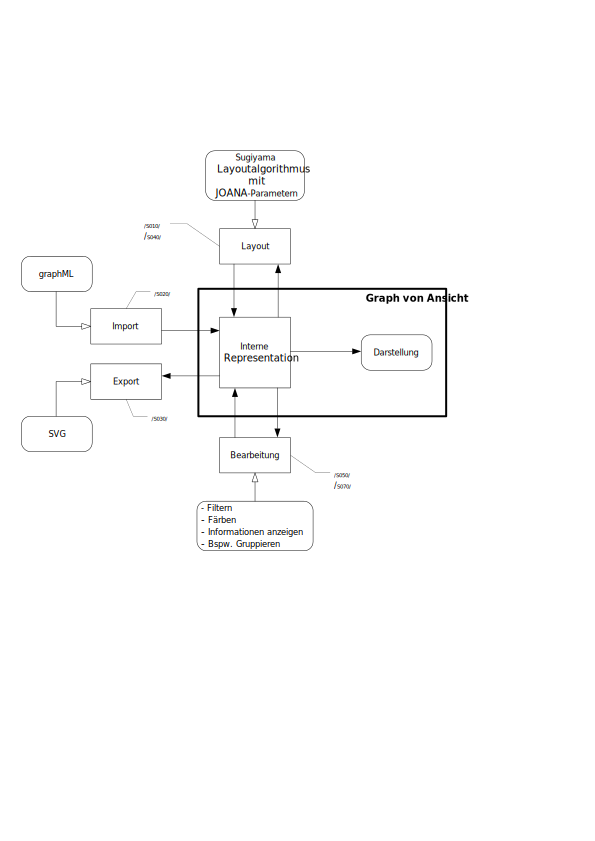
\includegraphics[width=380pt]{resourcen/plugin.pdf}
  \caption{Paketübersicht plugin}
  \label{fig:packge_plugin}
\end{figure}

Das Paket \textbf{plugin} bietet Interfaces für Plugins sowie einen \textbf{PluginManager} welcher die Plugins lädt, verwaltet und zur Verfügung stellt. Klassen die Interfaces dieses Plugins implementieren müssen sich beim laden, der Klasse die \textbf{Plugin} erweitert beim \textbf{PluginManager} registriert werden, um dann vom Programm verwendet werden zu können. Es bietet somit die Möglichkeit Funktionalität von außen zu laden und somit das Programm zu erweitern. \\
Ein \textbf{Importer} und ein \textbf{Exporter} Interface können implementiert werden um weitere File Importer oder Exporter hinzuzufügen. \\
Ein \textbf{LayoutAlgorithm} ist in der Lage einen Graphen zu layouten. Er hat \textbf{LayoutOption}s und \textbf{Constraint}s die eingestellt werden können, um die funktionsweise des Algorithmus zu beeinflussen. Die \textbf{LayoutOption}s können dann in einem \textbf{LayoutRegister} gespeichert werden. \\
\textbf{EdgeFilter}, \textbf{VertexFilter} und \textbf{FilterSet} erlauben es Plugins Filter für Kanten und Knoten zu definieren die bei Layouten und Darstellung unbeachtet bleiben. \\
\textbf{Workspace}s beschreiben eine Arbeitssituation in der spezifische Graphtypen verarbeitet werden können. Ein Beispiel hierfür ist der \textbf{JoanaWorkspace} im \textbf{joana} Paket. Ein Workspace definiert, welche Dateien mit welchem Importer importiert werden und ermöglicht so das öffnen spezifischer Graphtypen welche in generischen Formaten wie graphml gespeichert werden können. Dieses kann wiederum über \textbf{WorkspaceOption}s eingestellt werden.\\

\newpage

\section{sugiyama}

\begin{figure}[hb]
  \centering
  \includegraphics[width=380pt]{resourcen/sugiyama.pdf}
  \caption{Paketübersicht sugiyama}
  \label{fig:packge_sugiyama}
\end{figure}

Das Paket \textbf{sugiyama} bietet neben einer Implementierung des Sugiyama-Frameworks zum hierarchischen layouten eines gerichteten Graphen Schnittstellen zum ändern und austauschen einzelner Phasen dieses Frameworks.\\
Die fünf Phasen des Sugiyama-Frameworks: Kreise entfernen, Lagenzuordnung, Kreuzungsminimierung, Knotenpositionierung und Kantenzeichnen werden in dieser Reihenfolge durchlaufen und durch einen \textbf{SugiyamaLayoutAlgorithm} verwaltet und gesteuert. Die Klassen, die diese Schritte darstellen \textbf{CycleRemover}, \textbf{LayerAssigner}, \textbf{CrossMinimizer}, \textbf{VertexPositioner} und \textbf{EdgeDrawer} arbeiten auf einem \textbf{SugiyamaGraph}, welcher den zu layoutenden Graphen repräsentiert. Hierzu implementiert er die jeweiligen Interfaces, die diese Schritte fordern.\\
In der ersten Phase werden die Zykel des Graphen entfernt, indem die Richtungen einer minimalen Kantenmenge umgekehrt wird.\\
Anschließend wird jedem Knoten eine Lage zugewiesen, welche abhängig von der Anzahl der ein- und ausgehenden Kanten des Knotens, sowie der Länge des kürzesten Pfades des Knotens zu einem Knoten aus der ersten Lage ist. Zudem werden, falls eine Kante zwischen zwei Knoten mindestens eine Lage überspringt, in jede dieser Lagen ein \textbf{DummyVertex} ein.\\
In der dritten Phase wird die Anzahl der Kantenkreuzungen minimiert. Dazu werden jeweils in zwei aneinanderliegenden Lagen die Knoten beider Lagen umgeordnet.\\
In Phase Vier bekommen die Knoten feste Positionen in den Lagen zugewiesen\\
In der letzten Phase wird jeder \textbf{DummyVertex} entfernt und die Kanten werden gezeichnet. Zusätzlich werden die im ersten Schritt umgedrehten Kanten wieder in ihre ursprüngliche Richtung zurückversetzt.

\newpage

\section{joana}

\begin{figure}[hb]
  \centering
  \includegraphics[width=380pt]{resourcen/joana.pdf}
  \caption{Paketübersicht joana}
  \label{fig:packge_joana}
\end{figure}


Das \textbf{joana} Paket bietet Funktionalitäten zum Erstellen von Graphen samt Knoten und Kanten, sowie das Darstellen von \textbf{Methoden}- und \textbf{Callgraphen} in ihren eigenen Layouts.\\
Das \textbf{Workspace} bietet die Möglichkeit zum Einstellen und Speichern von Optionen, speziell für \textbf{JOANA-Graphen}.\\
Zudem ermöglicht das \textbf{joana} Paket die wiedererkennbare Darstellung von Feldzugriffen über das \textbf{FieldAccessLayout}, indem die Zugriffe immer ähnlich dargestellt werden.\\
\textbf{JoanaVertex} und \textbf{JoanaEdge} beinhalten Attribute, welche speziell auf die Eigenschaften abgestimmt sind, welche durch JOANA gesetzt werden.\\
\textbf{Callgraph} und \textbf{Methodengraph}(en) werden in einem speziellen \textbf{JoanaGraphModel} gespeichert.

\chapter{Differenzen zum Pflichtenheft}

Folgende Funktionale Anforderungen aus dem Abschnitt 4.2 Wunschfunktionen wurden noch nicht in den Entwurf mit aufgenommen:
\begin{itemize}
	\item /FA300/ Constraints hinzufügen
	\item /FA310/ Constraint bearbeiten
	\item /FA320/ Constraint löschen
	\item /FA330/ Steuerung über Tastaturkürzel
	\item /FA340/ Fortschrittsbalken bei Berechnung
	\item /FA350/ Eine Übersicht des angezeigten Graphen
	\item /FA360/ Änderung der Darstellung von Kanten
	\item /FA370/ Reload-Funktion
	\item /FA380/ Automatisierte Subgraph Auswahl
	\item /FA390/ Testen von Erreichbarkeit von Knoten
\end{itemize}

\clearpage

%\bibliography{referenzen}
\end{document}
